%&preformat-disser
\RequirePackage[l2tabu,orthodox]{nag} % Раскомментировав, можно в логе получать рекомендации относительно правильного использования пакетов и предупреждения об устаревших и нерекомендуемых пакетах
% Формат А4, 14pt (ГОСТ Р 7.0.11-2011, 5.3.6)
\documentclass[a4paper,14pt,oneside,openany]{memoir}

%%%%%%%%%%%%%%%%%%%%%%%%%%%%%%%%%%%%%%%%%%%%%%%%%%%%%%
%%%% Файл упрощённых настроек шаблона диссертации %%%%
%%%%%%%%%%%%%%%%%%%%%%%%%%%%%%%%%%%%%%%%%%%%%%%%%%%%%%

%%% Инициализирование переменных, не трогать!  %%%
\newcounter{tabcap}
\newcounter{tablaba}
\newcounter{tabtita}
%%%%%%%%%%%%%%%%%%%%%%%%%%%%%%%%%%%%%%%%%%%%%%%%%%

%%% Область упрощённого управления оформлением %%%


%% Подпись таблиц
\setcounter{tabcap}{0}              % 0 --- по ГОСТ, номер таблицы и название разделены тире, выровнены по левому краю, при необходимости на нескольких строках; 1 --- подпись таблицы не по ГОСТ, на двух и более строках, дальнейшие настройки: 
%Выравнивание первой строки, с подписью и номером
\setcounter{tablaba}{2}             % 0 --- по левому краю; 1 --- по центру; 2 --- по правому краю
%Выравнивание строк с самим названием таблицы
\setcounter{tabtita}{1}             % 0 --- по левому краю; 1 --- по центру; 2 --- по правому краю

%%% Цвета гиперссылок %%%
% Latex color definitions: http://latexcolor.com/
\definecolor{linkcolor}{rgb}{0.9,0,0}
\definecolor{citecolor}{rgb}{0,0.6,0}
\definecolor{urlcolor}{rgb}{0,0,1}
%\definecolor{linkcolor}{rgb}{0,0,0} %black
%\definecolor{citecolor}{rgb}{0,0,0} %black
%\definecolor{urlcolor}{rgb}{0,0,0} %black               % общие настройки шаблона
%%% Проверка используемого TeX-движка %%%
\usepackage{iftex}[2013/04/04]
\usepackage{multicol}
\newif\ifxetexorluatex   % определяем новый условный оператор (http://tex.stackexchange.com/a/47579/79756)
\ifXeTeX
    \xetexorluatextrue
\else
    \ifLuaTeX
        \xetexorluatextrue
    \else
        \xetexorluatexfalse
    \fi
\fi

\RequirePackage{etoolbox}[2015/08/02]               % Для продвинутой проверки разных условий

%%% Поля и разметка страницы %%%
\usepackage{pdflscape}                              % Для включения альбомных страниц
\usepackage{geometry}                               % Для последующего задания полей

%%% Математические пакеты %%%
\usepackage{amsthm,amsfonts,amsmath,amssymb,amscd}  % Математические дополнения от AMS
\usepackage{mathtools}                              % Добавляет окружение multlined

%%%% Установки для размера шрифта 14 pt %%%%
%% Формирование переменных и констант для сравнения (один раз для всех подключаемых файлов)%%
%% должно располагаться до вызова пакета fontspec или polyglossia, потому что они сбивают его работу
\newlength{\curtextsize}
\newlength{\bigtextsize}
\setlength{\bigtextsize}{13.9pt}

\makeatletter
%\show\f@size                                       % неплохо для отслеживания, но вызывает стопорение процесса, если документ компилируется без команды  -interaction=nonstopmode 
\setlength{\curtextsize}{\f@size pt}
\makeatother

%%% Кодировки и шрифты %%%
\ifxetexorluatex
    \usepackage{polyglossia}[2014/05/21]            % Поддержка многоязычности (fontspec подгружается автоматически)
\else
    \RequirePDFTeX                                  % tests for PDFTEX use and throws an error if a different engine is being used
   %%% Решение проблемы копирования текста в буфер кракозябрами
%    \input glyphtounicode.tex
%    \input glyphtounicode-cmr.tex %from pdfx package
%    \pdfgentounicode=1
    \usepackage{cmap}                               % Улучшенный поиск русских слов в полученном pdf-файле
    \defaulthyphenchar=127                          % Если стоит до fontenc, то переносы не впишутся в выделяемый текст при копировании его в буфер обмена
    \usepackage[T2A]{fontenc}                       % Поддержка русских букв
    \usepackage[utf8]{inputenc}[2014/04/30]         % Кодировка utf8
    \usepackage[english, russian]{babel}[2014/03/24]% Языки: русский, английский
    \IfFileExists{pscyr.sty}{\usepackage{pscyr}}{}  % Красивые русские шрифты
\fi

%%% Оформление абзацев %%%
\usepackage{indentfirst}                            % Красная строка

%%% Цвета %%%
\usepackage[dvipsnames,usenames]{color}
\usepackage{colortbl}
%\usepackage[dvipsnames, table, hyperref, cmyk]{xcolor} % Вероятно, более новый вариант, вместо предыдущих двух строк. Конвертация всех цветов в cmyk заложена как удовлетворение возможного требования типографий. Возможно конвертирование и в rgb.

%%% Таблицы %%%
\usepackage{longtable}                              % Длинные таблицы
\usepackage{multirow,makecell}                      % Улучшенное форматирование таблиц

%%% Общее форматирование
\usepackage{soulutf8}                               % Поддержка переносоустойчивых подчёркиваний и зачёркиваний
\usepackage{icomma}                                 % Запятая в десятичных дробях


%%% Гиперссылки %%%
\usepackage{hyperref}[2012/11/06]

%%% Изображения %%%
\usepackage{graphicx}[2014/04/25]                   % Подключаем пакет работы с графикой

%%% Списки %%%
\usepackage{enumitem}

%%% Подписи %%%
\usepackage{caption}[2013/05/02]                    % Для управления подписями (рисунков и таблиц) % Может управлять номерами рисунков и таблиц с caption %Иногда может управлять заголовками в списках рисунков и таблиц
\usepackage{subcaption}[2013/02/03]                 % Работа с подрисунками и подобным

%%% Счётчики %%%
\usepackage[figure,table]{totalcount}               % Счётчик рисунков и таблиц
\usepackage{totcount}                               % Пакет создания счётчиков на основе последнего номера подсчитываемого элемента (может требовать дважды компилировать документ)
\usepackage{totpages}                               % Счётчик страниц, совместимый с hyperref (ссылается на номер последней страницы). Желательно ставить последним пакетом в преамбуле

%%% Продвинутое управление групповыми ссылками (пока только формулами) %%%
\ifxetexorluatex
    \usepackage{cleveref}                           % cleveref корректно считывает язык из настроек polyglossia
\else
    \usepackage[russian]{cleveref}                  % cleveref имеет сложности со считыванием языка из babel. Такое решение русификации вывода выбрано вместо определения в documentclass из опасности что-то лишнее передать во все остальные пакеты, включая библиографию.
\fi
\creflabelformat{equation}{#2#1#3}                  % Формат по умолчанию ставил круглые скобки вокруг каждого номера ссылки, теперь просто номера ссылок без какого-либо дополнительного оформления


\ifnumequal{\value{draft}}{1}{% Черновик
    \usepackage[firstpage]{draftwatermark}
    \SetWatermarkText{DRAFT}
    \SetWatermarkFontSize{14pt}
    \SetWatermarkScale{15}
    \SetWatermarkAngle{45}
}{}



%part1
\newcommand{\rmnum}[1]{\romannumeral #1}
\newcommand{\Rmnum}[1]{\expandafter\@slowromancap\romannumeral #1@}
\newcommand*{\hm}[1]{#1\nobreak\discretionary{}%
	{\hbox{$\mathsurround=0pt #1$}}{}}% перенос арифметических знаков
\renewcommand{\Pr}{{\mathbf P}}
\newtheorem{corollary}{Следствие}[section]

\newcommand{\Mark}{\{(\Gamma_i, \varkappa_i); \hm{} i \geqslant 0\}}
\newcommand{\MarkThree}{\{(\Gamma_i, \varkappa_{3,i}); \hm{} i \geqslant 0\}}  % Пакеты общие для диссертации и автореферата
%%% Прикладные пакеты %%% 
%\usepackage{calc}               % Пакет для расчётов параметров, например длины         % Пакеты для диссертации
\usepackage{tabu, tabulary}  %таблицы с автоматически подбирающейся шириной столбцов
\usepackage{fr-longtable}    %ради \endlasthead

% Листинги с исходным кодом программ
\usepackage{fancyvrb}
\usepackage{listings}

% Русская традиция начертания греческих букв
\usepackage{upgreek} % прямые греческие ради русской традиции

% Микротипографика
%\ifnumequal{\value{draft}}{0}{% Только если у нас режим чистовика
%    \usepackage[final]{microtype}[2016/05/14] % улучшает представление букв и слов в строках, может помочь при наличии отдельно висящих слов
%}{}

% Отметка о версии черновика на каждой странице
% Чтобы работало надо в своей локальной копии по инструкции
% https://www.ctan.org/pkg/gitinfo2 создать небходимые файлы в папке
% ./git/hooks
% If you’re familiar with tweaking git, you can probably work it out for
% yourself. If not, I suggest you follow these steps:
% 1. First, you need a git repository and working tree. For this example,
% let’s suppose that the root of the working tree is in ~/compsci
% 2. Copy the file post-xxx-sample.txt (which is in the same folder of
% your TEX distribution as this pdf) into the git hooks directory in your
% working copy. In our example case, you should end up with a file called
% ~/compsci/.git/hooks/post-checkout
% 3. If you’re using a unix-like system, don’t forget to make the file executable.
% Just how you do this is outside the scope of this manual, but one
% possible way is with commands such as this:
% chmod g+x post-checkout.
% 4. Test your setup with “git checkout master” (or another suitable branch
% name). This should generate copies of gitHeadInfo.gin in the directories
% you intended.
% 5. Now make two more copies of this file in the same directory (hooks),
% calling them post-commit and post-merge, and you’re done. As before,
% users of unix-like systems should ensure these files are marked as
% executable.
\ifnumequal{\value{draft}}{1}{% Черновик
   \IfFileExists{.git/gitHeadInfo.gin}{                                        
      \usepackage[mark,pcount]{gitinfo2}
      \renewcommand{\gitMark}{rev.\gitAbbrevHash\quad\gitCommitterEmail\quad\gitAuthorIsoDate}
      \renewcommand{\gitMarkFormat}{\color{Gray}\small\bfseries}
   }{}
}{}        % Пакеты для специфических пользовательских задач

%%%%%%%%%%%%%%%%%%%%%%%%%%%%%%%%%%%%%%%%%%%%%%%%%%%%%%
%%%% Файл упрощённых настроек шаблона диссертации %%%%
%%%%%%%%%%%%%%%%%%%%%%%%%%%%%%%%%%%%%%%%%%%%%%%%%%%%%%

%%% Инициализирование переменных, не трогать!  %%%
\newcounter{tabcap}
\newcounter{tablaba}
\newcounter{tabtita}
%%%%%%%%%%%%%%%%%%%%%%%%%%%%%%%%%%%%%%%%%%%%%%%%%%

%%% Область упрощённого управления оформлением %%%


%% Подпись таблиц
\setcounter{tabcap}{0}              % 0 --- по ГОСТ, номер таблицы и название разделены тире, выровнены по левому краю, при необходимости на нескольких строках; 1 --- подпись таблицы не по ГОСТ, на двух и более строках, дальнейшие настройки: 
%Выравнивание первой строки, с подписью и номером
\setcounter{tablaba}{2}             % 0 --- по левому краю; 1 --- по центру; 2 --- по правому краю
%Выравнивание строк с самим названием таблицы
\setcounter{tabtita}{1}             % 0 --- по левому краю; 1 --- по центру; 2 --- по правому краю

%%% Цвета гиперссылок %%%
% Latex color definitions: http://latexcolor.com/
\definecolor{linkcolor}{rgb}{0.9,0,0}
\definecolor{citecolor}{rgb}{0,0.6,0}
\definecolor{urlcolor}{rgb}{0,0,1}
%\definecolor{linkcolor}{rgb}{0,0,0} %black
%\definecolor{citecolor}{rgb}{0,0,0} %black
%\definecolor{urlcolor}{rgb}{0,0,0} %black               % Упрощённые настройки шаблона

%%% Переопределение именований, чтобы можно было и в преамбуле использовать %%%
\renewcommand{\chaptername}{Глава}
\renewcommand{\appendixname}{Приложение} % (ГОСТ Р 7.0.11-2011, 5.7)
       % Переопределение именований, чтобы можно было и в преамбуле использовать
% Новые переменные, которые могут использоваться во всём проекте
% ГОСТ 7.0.11-2011
% 9.2 Оформление текста автореферата диссертации
% 9.2.1 Общая характеристика работы включает в себя следующие основные структурные
% элементы:
% актуальность темы исследования;
\newcommand{\actualityTXT}{Актуальность темы исследования.}
% степень ее разработанности;
\newcommand{\progressTXT}{Степень разработанности темы.}
% цели и задачи;
\newcommand{\aimTXT}{Цели и задачи работы.}
\newcommand{\tasksTXT}{задачи}
% научную новизну;
\newcommand{\noveltyTXT}{Научная новизна.}
% теоретическую и практическую значимость работы;
%\newcommand{\influenceTXT}{Теоретическая и практическая значимость}
% или чаще используют просто
\newcommand{\influenceTXT}{Теоретическая и практическая значимость.}
% методологию и методы исследования;
\newcommand{\methodsTXT}{Mетодология и методы исследования.}
% положения, выносимые на защиту;
\newcommand{\defpositionsTXT}{Основные положения, выносимые на~защиту.}
% степень достоверности и апробацию результатов.
\newcommand{\reliabilityTXT}{Достоверность}
\newcommand{\probationTXT}{Степень достоверности и апробация результатов.}

\newcommand{\contributionTXT}{Личный вклад автора.}
\newcommand{\passport}{\textbf{Соответствие паспорту специальности.}}
\newcommand{\publicationsTXT}{Публикации.}


\newcommand{\authorbibtitle}{Публикации автора по теме диссертации}
\newcommand{\fullbibtitle}{Список литературы} % (ГОСТ Р 7.0.11-2011, 4)
  % Новые переменные, которые могут использоваться во всём проекте

%%% Основные сведения %%%
\newcommand{\thesisAuthor}             % Диссертация, ФИО автора
{%
    \texorpdfstring{% \texorpdfstring takes two arguments and uses the first for (La)TeX and the second for pdf
        \todo{Кочеганов Виктор Михайлович}% так будет отображаться на титульном листе или в тексте, где будет использоваться переменная
    }{%
        Кочеганов, Виктор Михайлович % эта запись для свойств pdf-файла. В таком виде, если pdf будет обработан программами для сбора библиографических сведений, будет правильно представлена фамилия.
    }%
}
\newcommand{\thesisAuthorShort}        % Диссертация, ФИО автора инициалами
{\todo{В.М.~Кочеганов}}

\newcommand{\thesisUdk}                % Диссертация, УДК
{\todo{519.872}}
\newcommand{\thesisTitle}              % Диссертация, название
{\texorpdfstring{\todo{\MakeUppercase{
Исследование операции обслуживания конфликтных потоков в тандеме с задержкой по циклическому алгоритму с продлением}}}{Исследование операции обслуживания конфликтных потоков в тандеме с задержкой по циклическому алгоритму с продлением}}
\newcommand{\thesisSpecialtyNumber}    % Диссертация, специальность, номер
{\texorpdfstring{\todo{01.01.09}}{01.01.09}}
\newcommand{\thesisSpecialtyTitle}     % Диссертация, специальность, название
{\texorpdfstring{\todo{Дискретная математика и математическая кибернетика}}{Дискретная математика и математическая кибернетика}}
\newcommand{\thesisDegree}             % Диссертация, ученая степень
{\todo{кандидата физико-математических наук}}
\newcommand{\thesisDegreeShort}        % Диссертация, ученая степень, краткая запись
{\todo{канд. физ.-мат. наук}}
\newcommand{\thesisCity}               % Диссертация, город защиты
{\todo{Нижний Новгород}}
\newcommand{\thesisYear}               % Диссертация, год защиты
{\todo{2019}}
\newcommand{\thesisOrganization}       % Диссертация, организация
{\todo{Федеральное государственное автономное образовательное учреждение высшего образования «Национальный исследовательский Нижегородский государственный университет им.~Н.И.~Лобачевского»}}
\newcommand{\thesisOrganizationShort}  % Диссертация, краткое название организации для доклада
{\todo{ННГУ им.~Н.И.~Лобачевского}}

\newcommand{\thesisInOrganization}     % Диссертация, организация в предложном падеже: Работа выполнена в ...
{\todo{Федеральном государственном автономном образовательном учреждении высшего образования «Национальный исследовательский Нижегородский государственный университет им.~Н.И.~Лобачевского»}}

\newcommand{\supervisorFio}            % Научный руководитель, ФИО
{\todo{Зорин Андрей Владимирович}}
\newcommand{\supervisorRegalia}        % Научный руководитель, регалии
{\todo{доктор физико-математических наук, доцент}}
\newcommand{\supervisorFioShort}       % Научный руководитель, ФИО
{\todo{А.В.~Зорин}}
\newcommand{\supervisorRegaliaShort}   % Научный руководитель, регалии
{\todo{д.~ф.-м.~н.,~доц.}}
\newcommand{\supervisorJobPlace}      % Научный руководитель, место работы
{\todo{ФГАОУ ВО «Национальный исследовательский Нижегородский государственный университет им.~Н.И.~Лобачевского»}}
\newcommand{\supervisorJobPost}       % Научный руководитель, должность
{\todo{профессор кафедры программной инженерии Института информационных технологий, математики и механики}}


%\newcommand{\opponentOneFio}           % Оппонент 1, ФИО
%{\todo{Рыков Владимир Васильевич}}
%\newcommand{\opponentOneRegalia}       % Оппонент 1, регалии
%{\todo{доктор физико-математических наук, профессор}}
%\newcommand{\opponentOneJobPlace}      % Оппонент 1, место работы
%{\todo{ФГБОУ ВО <<Российский государственный университет нефти и газа (национальный исследовательский университет) имени И. М. Губкинa>>}}
%\newcommand{\opponentOneJobPost}       % Оппонент 1, должность
%{\todo{профессор кафедры прикладной математики и компьютерного моделирования факультета автоматики и вычислительной техники}}

\newcommand{\opponentOneFio}           % Оппонент 1, ФИО
{\todo{Оппонент Оппонентович Оппонентов1}}
\newcommand{\opponentOneRegalia}       % Оппонент 1, регалии
{\todo{доктор физико-математических наук, профессор}}
\newcommand{\opponentOneJobPlace}      % Оппонент 1, место работы
%{\todo{Федеральное государственное бюджетное образовательное учреждение высшего образования <<Московский государственный университет имени М.В.~Ломоносова>>}}
{\todo{ФГБОУ ВО <<Московский государственный университет имени М.В.~Ломоносова>>}}
\newcommand{\opponentOneJobPost}       % Оппонент 1, должность
{\todo{профессор кафедры математической статистики факультета вычислительной математики и кибернетики}}

\newcommand{\opponentTwoFio}           % Оппонент 2, ФИО
{\todo{Оппонент Оппонентович Оппонентов2}}
\newcommand{\opponentTwoRegalia}       % Оппонент 2, регалии
{\todo{доктор технических наук, профессор}}
\newcommand{\opponentTwoJobPlace}      % Оппонент 2, место работы
%{\todo{Федеральное государственное бюджетное образовательное учреждение высшего образования <<Волжский государственный университет водного транспорта>>}}
{\todo{ФГБОУ ВО <<Волжский государственный университет водного транспорта>>}}
\newcommand{\opponentTwoJobPost}       % Оппонент 2, должность
{\todo{заведующий кафедрой Информатики, систем управления и телекоммуникаций}}

\newcommand{\leadingOrganizationTitle} % Ведущая организация, дополнительные строки
%{\todo{Федеральное государственное автономное образовательное учреждение высшего образования <<Российский университет дружбы народов>>}}
{\todo{Кафедра прикладной информатики и теории вероятностей факультета физико-математических и естественных наук ФГАОУ ВО <<Российский университет дружбы народов>>}}

\newcommand{\defenseDate}              % Защита, дата
{\todo{20 апреля  2019~г.~в~14:40 часов}}
\newcommand{\defenseCouncilNumber}     % Защита, номер диссертационного совета
{\todo{Д\,212.166.20}}
\newcommand{\defenseCouncilTitle}      % Защита, учреждение диссертационного совета
{\todo{ФГАОУ ВО <<Национальный исследовательский Нижегородский государственный университет им.~Н.И.~Лобачевского>>}}
\newcommand{\defenseCouncilAddress}    % Защита, адрес учреждение диссертационного совета
{\todo{603950, г. Нижний Новгород, пр. Гагарина, д. 23}}
\newcommand{\defenseCouncilPhone}      % Телефон для справок
{\todo{+7~(0000)~00-00-00}}

\newcommand{\defenseSecretaryFio}      % Секретарь диссертационного совета, ФИО
{\todo{Кротов Николай Владимирович}}
\newcommand{\defenseSecretaryRegalia}  % Секретарь диссертационного совета, регалии
{\todo{кандидат физико-математических наук}}            % Для сокращений есть ГОСТы, например: ГОСТ Р 7.0.12-2011 + http://base.garant.ru/179724/#block_30000

\newcommand{\synopsisLibrary}          % Автореферат, название библиотеки
{\todo{Фундаментальная библиотека ФГАОУ ВО «Национального исследовательского Нижегородского государственного университета им.~Н.И.~Лобачевского»}}
\newcommand{\synopsisDate}             % Автореферат, дата рассылки
{\todo{DD mmmmmmmm YYYY года}}

% To avoid conflict with beamer class use \providecommand
\providecommand{\keywords}%            % Ключевые слова для метаданных PDF диссертации и автореферата
{}      % Основные сведения
%%% Кодировки и шрифты %%%
\ifxetexorluatex
    \setmainlanguage[babelshorthands=true]{russian}  % Язык по-умолчанию русский с поддержкой приятных команд пакета babel
    \setotherlanguage{english}                       % Дополнительный язык = английский (в американской вариации по-умолчанию)
    \setmonofont{Courier New}
    \newfontfamily\cyrillicfonttt{Courier New}
    \ifXeTeX
        \defaultfontfeatures{Ligatures=TeX,Mapping=tex-text}
    \else
        \defaultfontfeatures{Ligatures=TeX}
    \fi
    \setmainfont{Times New Roman}
    \newfontfamily\cyrillicfont{Times New Roman}
    \setsansfont{Arial}
    \newfontfamily\cyrillicfontsf{Arial}
\else
    \IfFileExists{pscyr.sty}{\renewcommand{\rmdefault}{ftm}}{}
\fi

%%% Подписи %%%
\captionsetup{%
singlelinecheck=off,                % Многострочные подписи, например у таблиц
skip=2pt,                           % Вертикальная отбивка между подписью и содержимым рисунка или таблицы определяется ключом
justification=centering,            % Центрирование подписей, заданных командой \caption
}

%%% Рисунки %%%
\DeclareCaptionLabelSeparator*{emdash}{~--- }             % (ГОСТ 2.105, 4.3.1)
\captionsetup[figure]{labelsep=emdash,position=bottom}

%%% Таблицы %%%
\ifnumequal{\value{tabcap}}{0}{%
    \newcommand{\tabcapalign}{\raggedright}  % по левому краю страницы или аналога parbox

    \DeclareCaptionFormat{tablecaption}{\tabcapalign #1#2#3}
    \captionsetup[table]{labelsep=emdash}                       % тире как разделитель идентификатора с номером от наименования
}{%
    \ifnumequal{\value{tablaba}}{0}{%
        \newcommand{\tabcapalign}{\raggedright}  % по левому краю страницы или аналога parbox
    }{}

    \ifnumequal{\value{tablaba}}{1}{%
        \newcommand{\tabcapalign}{\centering}    % по центру страницы или аналога parbox
    }{}

    \ifnumequal{\value{tablaba}}{2}{%
        \newcommand{\tabcapalign}{\raggedleft}   % по правому краю страницы или аналога parbox
    }{}

    \ifnumequal{\value{tabtita}}{0}{%
        \newcommand{\tabtitalign}{\raggedright}  % по левому краю страницы или аналога parbox
    }{}

    \ifnumequal{\value{tabtita}}{1}{%
        \newcommand{\tabtitalign}{\centering}    % по центру страницы или аналога parbox
    }{}

    \ifnumequal{\value{tabtita}}{2}{%
        \newcommand{\tabtitalign}{\raggedleft}   % по правому краю страницы или аналога parbox
    }{}

    \DeclareCaptionFormat{tablecaption}{\tabcapalign #1#2\par%  % Идентификатор таблицы на отдельной строке
        \tabtitalign{#3}}                                       % Наименование таблицы строкой ниже
    \captionsetup[table]{labelsep=space}                        % пробельный разделитель идентификатора с номером от наименования
}
\DeclareCaptionFormat{tablenocaption}{\tabcapalign #1\strut}    % Наименование таблицы отсутствует

\captionsetup[table]{format=tablecaption,singlelinecheck=off,position=top,skip=0pt}  % многострочные наименования и прочее
\DeclareCaptionLabelFormat{continued}{Продолжение таблицы~#2}

%%% Подписи подрисунков %%%
\renewcommand{\thesubfigure}{\asbuk{subfigure}}           % Буквенные номера подрисунков
\captionsetup[subfigure]{font={normalsize},               % Шрифт подписи названий подрисунков (не отличается от основного)
    labelformat=brace,                                    % Формат обозначения подрисунка
    justification=centering,                              % Выключка подписей (форматирование), один из вариантов            
}
%\DeclareCaptionFont{font12pt}{\fontsize{12pt}{13pt}\selectfont} % объявляем шрифт 12pt для использования в подписях, тут же надо интерлиньяж объявлять, если не наследуется
%\captionsetup[subfigure]{font={font12pt}}                 % Шрифт подписи названий подрисунков (всегда 12pt)

%%% Настройки гиперссылок %%%
\ifLuaTeX
    \hypersetup{
        unicode,                % Unicode encoded PDF strings
    }
\fi

\hypersetup{
    linktocpage=true,           % ссылки с номера страницы в оглавлении, списке таблиц и списке рисунков
%    linktoc=all,                % both the section and page part are links
%    pdfpagelabels=false,        % set PDF page labels (true|false)
    plainpages=false,           % Forces page anchors to be named by the Arabic form  of the page number, rather than the formatted form
    colorlinks,                 % ссылки отображаются раскрашенным текстом, а не раскрашенным прямоугольником, вокруг текста
    linkcolor={blue},%{black},      % цвет ссылок типа ref, eqref и подобных
    citecolor={blue},%{black},      % цвет ссылок-цитат
    urlcolor={black},%{blue},        % цвет гиперссылок
%    hidelinks,                  % Hide links (removing color and border)
    pdftitle={\thesisTitle},    % Заголовок
    pdfauthor={\thesisAuthor},  % Автор
    pdfsubject={\thesisSpecialtyNumber\ \thesisSpecialtyTitle},      % Тема
%    pdfcreator={Создатель},     % Создатель, Приложение
%    pdfproducer={Производитель},% Производитель, Производитель PDF
    pdfkeywords={\keywords},    % Ключевые слова
    pdflang={ru},
}
\ifnumequal{\value{draft}}{1}{% Черновик
    \hypersetup{
        draft,
    }
}{}

%%% Шаблон %%%
\DeclareRobustCommand{\todo}{\textcolor{black}}       % решаем проблему превращения названия цвета в результате \MakeUppercase, http://tex.stackexchange.com/a/187930/79756 , \DeclareRobustCommand protects \todo from expanding inside \MakeUppercase
\AtBeginDocument{%
    \setlength{\parindent}{2.5em}                   % Абзацный отступ. Должен быть одинаковым по всему тексту и равен пяти знакам (ГОСТ Р 7.0.11-2011, 5.3.7).
}

%%% Списки %%%
% Используем короткое тире (endash) для ненумерованных списков (ГОСТ 2.105-95, пункт 4.1.7, требует дефиса, но так лучше смотрится)
\renewcommand{\labelitemi}{\normalfont\bfseries{--}}

% Перечисление строчными буквами латинского алфавита (ГОСТ 2.105-95, 4.1.7)
%\renewcommand{\theenumi}{\alph{enumi}}
%\renewcommand{\labelenumi}{\theenumi)} 

% Перечисление строчными буквами русского алфавита (ГОСТ 2.105-95, 4.1.7)
%\makeatletter
%\AddEnumerateCounter{\asbuk}{\russian@alph}{щ}      % Управляем списками/перечислениями через пакет enumitem, а он 'не знает' про asbuk, потому 'учим' его
%\makeatother
%\renewcommand{\theenumi}{\asbuk{enumi}}
%\renewcommand{\labelenumi}{\theenumi)} 

\setlist{nosep,%                                    % Единый стиль для всех списков (пакет enumitem), без дополнительных интервалов.
    labelindent=\parindent,leftmargin=*%            % Каждый пункт, подпункт и перечисление записывают с абзацного отступа (ГОСТ 2.105-95, 4.1.8)
}
    % Стили общие для диссертации и автореферата
%%% Изображения %%%
\graphicspath{{images/}{Dissertation/images/}}         % Пути к изображениям

%%% Макет страницы %%%
% Выставляем значения полей (ГОСТ 7.0.11-2011, 5.3.7)
\geometry{a4paper,top=2cm,bottom=2cm,left=2.5cm,right=1cm,nofoot,nomarginpar} %,showframe
\setlength{\topskip}{0pt}   %размер дополнительного верхнего поля

%%% Интервалы %%%
%% По ГОСТ Р 7.0.11-2011, пункту 5.3.6 требуется полуторный интервал
%% Реализация средствами класса (на основе setspace) ближе к типографской классике.
%% И правит сразу и в таблицах (если со звёздочкой) 
%\DoubleSpacing*     % Двойной интервал
\OnehalfSpacing*    % Полуторный интервал
%\setSpacing{1.42}   % Полуторный интервал, подобный Ворду (возможно, стоит включать вместе с предыдущей строкой)

%%% Выравнивание и переносы %%%
%% http://tex.stackexchange.com/questions/241343/what-is-the-meaning-of-fussy-sloppy-emergencystretch-tolerance-hbadness
%% http://www.latex-community.org/forum/viewtopic.php?p=70342#p70342
\tolerance 1414
\hbadness 1414
\emergencystretch 1.5em % В случае проблем регулировать в первую очередь
\hfuzz 0.3pt
\vfuzz \hfuzz
%\raggedbottom
%\sloppy                 % Избавляемся от переполнений
\clubpenalty=10000      % Запрещаем разрыв страницы после первой строки абзаца
\widowpenalty=10000     % Запрещаем разрыв страницы после последней строки абзаца

%%% Блок управления параметрами для выравнивания заголовков в тексте %%%
\newlength{\otstuplen}
\setlength{\otstuplen}{\theotstup\parindent}
\ifnumequal{\value{headingalign}}{0}{% выравнивание заголовков в тексте
    \newcommand{\hdngalign}{\centering}                % по центру
    \newcommand{\hdngaligni}{}% по центру
    \setlength{\otstuplen}{0pt}
}{%
    \newcommand{\hdngalign}{}                 % по левому краю
    \newcommand{\hdngaligni}{\hspace{\otstuplen}}      % по левому краю
} % В обоих случаях вроде бы без переноса, как и надо (ГОСТ Р 7.0.11-2011, 5.3.5)

%%% Оглавление %%%
\renewcommand{\cftchapterdotsep}{\cftdotsep}                % отбивка точками до номера страницы начала главы/раздела

%% Переносить слова в заголовке не допускается (ГОСТ Р 7.0.11-2011, 5.3.5). Заголовки в оглавлении должны точно повторять заголовки в тексте (ГОСТ Р 7.0.11-2011, 5.2.3). Прямого указания на запрет переносов в оглавлении нет, но по той же логике невнесения искажений в смысл, лучше в оглавлении не переносить:
\setrmarg{2.55em plus1fil}                             %To have the (sectional) titles in the ToC, etc., typeset ragged right with no hyphenation
\renewcommand{\cftchapterpagefont}{\normalfont}        % нежирные номера страниц у глав в оглавлении
\renewcommand{\cftchapterleader}{\cftdotfill{\cftchapterdotsep}}% нежирные точки до номеров страниц у глав в оглавлении
%\renewcommand{\cftchapterfont}{}                       % нежирные названия глав в оглавлении

\ifnumgreater{\value{headingdelim}}{0}{%
    \renewcommand\cftchapteraftersnum{.\space}       % добавляет точку с пробелом после номера раздела в оглавлении
}{}
\ifnumgreater{\value{headingdelim}}{1}{%
    \renewcommand\cftsectionaftersnum{.\space}       % добавляет точку с пробелом после номера подраздела в оглавлении
    \renewcommand\cftsubsectionaftersnum{.\space}    % добавляет точку с пробелом после номера подподраздела в оглавлении
    \renewcommand\cftsubsubsectionaftersnum{.\space} % добавляет точку с пробелом после номера подподподраздела в оглавлении
    \AtBeginDocument{% без этого polyglossia сама всё переопределяет
        \setsecnumformat{\csname the#1\endcsname.\space}
    }
}{%
    \AtBeginDocument{% без этого polyglossia сама всё переопределяет
        \setsecnumformat{\csname the#1\endcsname\quad}
    }
}

\ifnumequal{\value{pgnum}}{1}{%
    \addtocontents{toc}{~\hfill{Стр.}\par}% добавить Стр. над номерами страниц
}{}

\renewcommand*{\cftappendixname}{\appendixname\space} % Слово Приложение в оглавлении

%%% Колонтитулы %%%
% Порядковый номер страницы печатают на середине верхнего поля страницы (ГОСТ Р 7.0.11-2011, 5.3.8)
\makeevenhead{plain}{}{\thepage}{}
\makeoddhead{plain}{}{\thepage}{}
\makeevenfoot{plain}{}{}{}
\makeoddfoot{plain}{}{}{}
\pagestyle{plain}

%%% Оформление заголовков глав, разделов, подразделов %%%
%% Работа должна быть выполнена ... размером шрифта 12-14 пунктов (ГОСТ Р 7.0.11-2011, 5.3.8). То есть не должно быть надписей шрифтом более 14. Так и поставим.
%% Эти установки будут давать одинаковый результат независимо от выбора базовым шрифтом 12 пт или 14 пт
\newcommand{\basegostsectionfont}{\fontsize{14pt}{16pt}\selectfont\bfseries}

\makechapterstyle{thesisgost}{%
    \chapterstyle{default}
    \setlength{\beforechapskip}{0pt}
    \setlength{\midchapskip}{0pt}
    \setlength{\afterchapskip}{\theintvl\curtextsize}
    \renewcommand*{\chapnamefont}{\basegostsectionfont}
    \renewcommand*{\chapnumfont}{\basegostsectionfont}
    \renewcommand*{\chaptitlefont}{\basegostsectionfont}
    \renewcommand*{\chapterheadstart}{}
    \ifnumgreater{\value{headingdelim}}{0}{%
        \renewcommand*{\afterchapternum}{.\space}   % добавляет точку с пробелом после номера раздела
    }{%
        \renewcommand*{\afterchapternum}{\quad}     % добавляет \quad после номера раздела
    }
    \renewcommand*{\printchapternum}{\hdngaligni\hdngalign\chapnumfont \thechapter}
    \renewcommand*{\printchaptername}{}
    \renewcommand*{\printchapternonum}{\hdngaligni\hdngalign}
}

\makeatletter
\makechapterstyle{thesisgostchapname}{%
    \chapterstyle{thesisgost}
    \renewcommand*{\printchapternum}{\chapnumfont \thechapter}
    \renewcommand*{\printchaptername}{\hdngaligni\hdngalign\chapnamefont \@chapapp} %
}
\makeatother

\chapterstyle{thesisgost}

\setsecheadstyle{\basegostsectionfont\hdngalign}
\setsecindent{\otstuplen}

\setsubsecheadstyle{\basegostsectionfont\hdngalign}
\setsubsecindent{\otstuplen}

\setsubsubsecheadstyle{\basegostsectionfont\hdngalign}
\setsubsubsecindent{\otstuplen}

\sethangfrom{\noindent #1} %все заголовки подразделов центрируются с учетом номера, как block 

\ifnumequal{\value{chapstyle}}{1}{%
    \chapterstyle{thesisgostchapname}
    \renewcommand*{\cftchaptername}{\chaptername\space} % будет вписано слово Глава перед каждым номером раздела в оглавлении
}{}%

%%% Интервалы между заголовками
\setbeforesecskip{\theintvl\curtextsize}% Заголовки отделяют от текста сверху и снизу тремя интервалами (ГОСТ Р 7.0.11-2011, 5.3.5).
\setaftersecskip{\theintvl\curtextsize}
\setbeforesubsecskip{\theintvl\curtextsize}
\setaftersubsecskip{\theintvl\curtextsize}
\setbeforesubsubsecskip{\theintvl\curtextsize}
\setaftersubsubsecskip{\theintvl\curtextsize}

%%% Блок дополнительного управления размерами заголовков
\ifnumequal{\value{headingsize}}{1}{% Пропорциональные заголовки и базовый шрифт 14 пт
    \renewcommand{\basegostsectionfont}{\large\bfseries}
    \renewcommand*{\chapnamefont}{\Large\bfseries}
    \renewcommand*{\chapnumfont}{\Large\bfseries}
    \renewcommand*{\chaptitlefont}{\Large\bfseries}
}{}

%%% Счётчики %%%

%% Упрощённые настройки шаблона диссертации: нумерация формул, таблиц, рисунков
\ifnumequal{\value{contnumeq}}{1}{%
    \counterwithout{equation}{chapter} % Убираем связанность номера формулы с номером главы/раздела
}{}
\ifnumequal{\value{contnumfig}}{1}{%
    \counterwithout{figure}{chapter}   % Убираем связанность номера рисунка с номером главы/раздела
}{}
\ifnumequal{\value{contnumtab}}{1}{%
    \counterwithout{table}{chapter}    % Убираем связанность номера таблицы с номером главы/раздела
}{}


%%http://www.linux.org.ru/forum/general/6993203#comment-6994589 (используется totcount)
\makeatletter
\def\formbytotal#1#2#3#4#5{%
    \newcount\@c
    \@c\totvalue{#1}\relax
    \newcount\@last
    \newcount\@pnul
    \@last\@c\relax
    \divide\@last 10
    \@pnul\@last\relax
    \divide\@pnul 10
    \multiply\@pnul-10
    \advance\@pnul\@last
    \multiply\@last-10
    \advance\@last\@c
    \total{#1}~#2%
    \ifnum\@pnul=1#5\else%
    \ifcase\@last#5\or#3\or#4\or#4\or#4\else#5\fi
    \fi
}
\makeatother

\AtBeginDocument{
%% регистрируем счётчики в системе totcounter
    \regtotcounter{totalcount@figure}
    \regtotcounter{totalcount@table}       % Если иным способом поставить в преамбуле то ошибка в числе таблиц
    \regtotcounter{TotPages}               % Если иным способом поставить в преамбуле то ошибка в числе страниц
}

%%% Правильная нумерация приложений %%%
%% По ГОСТ 2.105, п. 4.3.8 Приложения обозначают заглавными буквами русского алфавита,
%% начиная с А, за исключением букв Ё, З, Й, О, Ч, Ь, Ы, Ъ.
%% Здесь также переделаны все нумерации русскими буквами.
\ifxetexorluatex
    \makeatletter
    \def\russian@Alph#1{\ifcase#1\or
       А\or Б\or В\or Г\or Д\or Е\or Ж\or
       И\or К\or Л\or М\or Н\or
       П\or Р\or С\or Т\or У\or Ф\or Х\or
       Ц\or Ш\or Щ\or Э\or Ю\or Я\else\xpg@ill@value{#1}{russian@Alph}\fi}
    \def\russian@alph#1{\ifcase#1\or
       а\or б\or в\or г\or д\or е\or ж\or
       и\or к\or л\or м\or н\or
       п\or р\or с\or т\or у\or ф\or х\or
       ц\or ш\or щ\or э\or ю\or я\else\xpg@ill@value{#1}{russian@alph}\fi}
    \makeatother
\else
    \makeatletter
    \if@uni@ode
      \def\russian@Alph#1{\ifcase#1\or
        А\or Б\or В\or Г\or Д\or Е\or Ж\or
        И\or К\or Л\or М\or Н\or
        П\or Р\or С\or Т\or У\or Ф\or Х\or
        Ц\or Ш\or Щ\or Э\or Ю\or Я\else\@ctrerr\fi}
    \else
      \def\russian@Alph#1{\ifcase#1\or
        \CYRA\or\CYRB\or\CYRV\or\CYRG\or\CYRD\or\CYRE\or\CYRZH\or
        \CYRI\or\CYRK\or\CYRL\or\CYRM\or\CYRN\or
        \CYRP\or\CYRR\or\CYRS\or\CYRT\or\CYRU\or\CYRF\or\CYRH\or
        \CYRC\or\CYRSH\or\CYRSHCH\or\CYREREV\or\CYRYU\or
        \CYRYA\else\@ctrerr\fi}
    \fi
    \if@uni@ode
      \def\russian@alph#1{\ifcase#1\or
        а\or б\or в\or г\or д\or е\or ж\or
        и\or к\or л\or м\or н\or
        п\or р\or с\or т\or у\or ф\or х\or
        ц\or ш\or щ\or э\or ю\or я\else\@ctrerr\fi}
    \else
      \def\russian@alph#1{\ifcase#1\or
        \cyra\or\cyrb\or\cyrv\or\cyrg\or\cyrd\or\cyre\or\cyrzh\or
        \cyri\or\cyrk\or\cyrl\or\cyrm\or\cyrn\or
        \cyrp\or\cyrr\or\cyrs\or\cyrt\or\cyru\or\cyrf\or\cyrh\or
        \cyrc\or\cyrsh\or\cyrshch\or\cyrerev\or\cyryu\or
        \cyrya\else\@ctrerr\fi}
    \fi
    \makeatother
\fi           % Стили для диссертации
% для вертикального центрирования ячеек в tabulary
\def\zz{\ifx\[$\else\aftergroup\zzz\fi}
%$ \] % <-- чиним подсветку синтаксиса в некоторых редакторах
\def\zzz{\setbox0\lastbox
\dimen0\dimexpr\extrarowheight + \ht0-\dp0\relax
\setbox0\hbox{\raise-.5\dimen0\box0}%
\ht0=\dimexpr\ht0+\extrarowheight\relax
\dp0=\dimexpr\dp0+\extrarowheight\relax 
\box0
}



\lstdefinelanguage{Renhanced}%
{keywords={abbreviate,abline,abs,acos,acosh,action,add1,add,%
        aggregate,alias,Alias,alist,all,anova,any,aov,aperm,append,apply,%
        approx,approxfun,apropos,Arg,args,array,arrows,as,asin,asinh,%
        atan,atan2,atanh,attach,attr,attributes,autoload,autoloader,ave,%
        axis,backsolve,barplot,basename,besselI,besselJ,besselK,besselY,%
        beta,binomial,body,box,boxplot,break,browser,bug,builtins,bxp,by,%
        c,C,call,Call,case,cat,category,cbind,ceiling,character,char,%
        charmatch,check,chol,chol2inv,choose,chull,class,close,cm,codes,%
        coef,coefficients,co,col,colnames,colors,colours,commandArgs,%
        comment,complete,complex,conflicts,Conj,contents,contour,%
        contrasts,contr,control,helmert,contrib,convolve,cooks,coords,%
        distance,coplot,cor,cos,cosh,count,fields,cov,covratio,wt,CRAN,%
        create,crossprod,cummax,cummin,cumprod,cumsum,curve,cut,cycle,D,%
        data,dataentry,date,dbeta,dbinom,dcauchy,dchisq,de,debug,%
        debugger,Defunct,default,delay,delete,deltat,demo,de,density,%
        deparse,dependencies,Deprecated,deriv,description,detach,%
        dev2bitmap,dev,cur,deviance,off,prev,,dexp,df,dfbetas,dffits,%
        dgamma,dgeom,dget,dhyper,diag,diff,digamma,dim,dimnames,dir,%
        dirname,dlnorm,dlogis,dnbinom,dnchisq,dnorm,do,dotplot,double,%
        download,dpois,dput,drop,drop1,dsignrank,dt,dummy,dump,dunif,%
        duplicated,dweibull,dwilcox,dyn,edit,eff,effects,eigen,else,%
        emacs,end,environment,env,erase,eval,equal,evalq,example,exists,%
        exit,exp,expand,expression,External,extract,extractAIC,factor,%
        fail,family,fft,file,filled,find,fitted,fivenum,fix,floor,for,%
        For,formals,format,formatC,formula,Fortran,forwardsolve,frame,%
        frequency,ftable,ftable2table,function,gamma,Gamma,gammaCody,%
        gaussian,gc,gcinfo,gctorture,get,getenv,geterrmessage,getOption,%
        getwd,gl,glm,globalenv,gnome,GNOME,graphics,gray,grep,grey,grid,%
        gsub,hasTsp,hat,heat,help,hist,home,hsv,httpclient,I,identify,if,%
        ifelse,Im,image,\%in\%,index,influence,measures,inherits,install,%
        installed,integer,interaction,interactive,Internal,intersect,%
        inverse,invisible,IQR,is,jitter,kappa,kronecker,labels,lapply,%
        layout,lbeta,lchoose,lcm,legend,length,levels,lgamma,library,%
        licence,license,lines,list,lm,load,local,locator,log,log10,log1p,%
        log2,logical,loglin,lower,lowess,ls,lsfit,lsf,ls,machine,Machine,%
        mad,mahalanobis,make,link,margin,match,Math,matlines,mat,matplot,%
        matpoints,matrix,max,mean,median,memory,menu,merge,methods,min,%
        missing,Mod,mode,model,response,mosaicplot,mtext,mvfft,na,nan,%
        names,omit,nargs,nchar,ncol,NCOL,new,next,NextMethod,nextn,%
        nlevels,nlm,noquote,NotYetImplemented,NotYetUsed,nrow,NROW,null,%
        numeric,\%o\%,objects,offset,old,on,Ops,optim,optimise,optimize,%
        options,or,order,ordered,outer,package,packages,page,pairlist,%
        pairs,palette,panel,par,parent,parse,paste,path,pbeta,pbinom,%
        pcauchy,pchisq,pentagamma,persp,pexp,pf,pgamma,pgeom,phyper,pico,%
        pictex,piechart,Platform,plnorm,plogis,plot,pmatch,pmax,pmin,%
        pnbinom,pnchisq,pnorm,points,poisson,poly,polygon,polyroot,pos,%
        postscript,power,ppoints,ppois,predict,preplot,pretty,Primitive,%
        print,prmatrix,proc,prod,profile,proj,prompt,prop,provide,%
        psignrank,ps,pt,ptukey,punif,pweibull,pwilcox,q,qbeta,qbinom,%
        qcauchy,qchisq,qexp,qf,qgamma,qgeom,qhyper,qlnorm,qlogis,qnbinom,%
        qnchisq,qnorm,qpois,qqline,qqnorm,qqplot,qr,Q,qty,qy,qsignrank,%
        qt,qtukey,quantile,quasi,quit,qunif,quote,qweibull,qwilcox,%
        rainbow,range,rank,rbeta,rbind,rbinom,rcauchy,rchisq,Re,read,csv,%
        csv2,fwf,readline,socket,real,Recall,rect,reformulate,regexpr,%
        relevel,remove,rep,repeat,replace,replications,report,require,%
        resid,residuals,restart,return,rev,rexp,rf,rgamma,rgb,rgeom,R,%
        rhyper,rle,rlnorm,rlogis,rm,rnbinom,RNGkind,rnorm,round,row,%
        rownames,rowsum,rpois,rsignrank,rstandard,rstudent,rt,rug,runif,%
        rweibull,rwilcox,sample,sapply,save,scale,scan,scan,screen,sd,se,%
        search,searchpaths,segments,seq,sequence,setdiff,setequal,set,%
        setwd,show,sign,signif,sin,single,sinh,sink,solve,sort,source,%
        spline,splinefun,split,sqrt,stars,start,stat,stem,step,stop,%
        storage,strstrheight,stripplot,strsplit,structure,strwidth,sub,%
        subset,substitute,substr,substring,sum,summary,sunflowerplot,svd,%
        sweep,switch,symbol,symbols,symnum,sys,status,system,t,table,%
        tabulate,tan,tanh,tapply,tempfile,terms,terrain,tetragamma,text,%
        time,title,topo,trace,traceback,transform,tri,trigamma,trunc,try,%
        ts,tsp,typeof,unclass,undebug,undoc,union,unique,uniroot,unix,%
        unlink,unlist,unname,untrace,update,upper,url,UseMethod,var,%
        variable,vector,Version,vi,warning,warnings,weighted,weights,%
        which,while,window,write,\%x\%,x11,X11,xedit,xemacs,xinch,xor,%
        xpdrows,xy,xyinch,yinch,zapsmall,zip},%
    otherkeywords={!,!=,~,$,*,\%,\&,\%/\%,\%*\%,\%\%,<-,<<-},%$
    alsoother={._$},%$
    sensitive,%
    morecomment=[l]\#,%
    morestring=[d]",%
    morestring=[d]'% 2001 Robert Denham
}%

%решаем проблему с кириллицей в комментариях (в pdflatex) https://tex.stackexchange.com/a/103712/79756
\lstset{extendedchars=true,literate={Ö}{{\"O}}1
    {Ä}{{\"A}}1
    {Ü}{{\"U}}1
    {ß}{{\ss}}1
    {ü}{{\"u}}1
    {ä}{{\"a}}1
    {ö}{{\"o}}1
    {~}{{\textasciitilde}}1
    {а}{{\selectfont\char224}}1
    {б}{{\selectfont\char225}}1
    {в}{{\selectfont\char226}}1
    {г}{{\selectfont\char227}}1
    {д}{{\selectfont\char228}}1
    {е}{{\selectfont\char229}}1
    {ё}{{\"e}}1
    {ж}{{\selectfont\char230}}1
    {з}{{\selectfont\char231}}1
    {и}{{\selectfont\char232}}1
    {й}{{\selectfont\char233}}1
    {к}{{\selectfont\char234}}1
    {л}{{\selectfont\char235}}1
    {м}{{\selectfont\char236}}1
    {н}{{\selectfont\char237}}1
    {о}{{\selectfont\char238}}1
    {п}{{\selectfont\char239}}1
    {р}{{\selectfont\char240}}1
    {с}{{\selectfont\char241}}1
    {т}{{\selectfont\char242}}1
    {у}{{\selectfont\char243}}1
    {ф}{{\selectfont\char244}}1
    {х}{{\selectfont\char245}}1
    {ц}{{\selectfont\char246}}1
    {ч}{{\selectfont\char247}}1
    {ш}{{\selectfont\char248}}1
    {щ}{{\selectfont\char249}}1
    {ъ}{{\selectfont\char250}}1
    {ы}{{\selectfont\char251}}1
    {ь}{{\selectfont\char252}}1
    {э}{{\selectfont\char253}}1
    {ю}{{\selectfont\char254}}1
    {я}{{\selectfont\char255}}1
    {А}{{\selectfont\char192}}1
    {Б}{{\selectfont\char193}}1
    {В}{{\selectfont\char194}}1
    {Г}{{\selectfont\char195}}1
    {Д}{{\selectfont\char196}}1
    {Е}{{\selectfont\char197}}1
    {Ё}{{\"E}}1
    {Ж}{{\selectfont\char198}}1
    {З}{{\selectfont\char199}}1
    {И}{{\selectfont\char200}}1
    {Й}{{\selectfont\char201}}1
    {К}{{\selectfont\char202}}1
    {Л}{{\selectfont\char203}}1
    {М}{{\selectfont\char204}}1
    {Н}{{\selectfont\char205}}1
    {О}{{\selectfont\char206}}1
    {П}{{\selectfont\char207}}1
    {Р}{{\selectfont\char208}}1
    {С}{{\selectfont\char209}}1
    {Т}{{\selectfont\char210}}1
    {У}{{\selectfont\char211}}1
    {Ф}{{\selectfont\char212}}1
    {Х}{{\selectfont\char213}}1
    {Ц}{{\selectfont\char214}}1
    {Ч}{{\selectfont\char215}}1
    {Ш}{{\selectfont\char216}}1
    {Щ}{{\selectfont\char217}}1
    {Ъ}{{\selectfont\char218}}1
    {Ы}{{\selectfont\char219}}1
    {Ь}{{\selectfont\char220}}1
    {Э}{{\selectfont\char221}}1
    {Ю}{{\selectfont\char222}}1
    {Я}{{\selectfont\char223}}1
    {і}{{\selectfont\char105}}1
    {ї}{{\selectfont\char168}}1
    {є}{{\selectfont\char185}}1
    {ґ}{{\selectfont\char160}}1
    {І}{{\selectfont\char73}}1
    {Ї}{{\selectfont\char136}}1
    {Є}{{\selectfont\char153}}1
    {Ґ}{{\selectfont\char128}}1
}

% Ширина текста минус ширина надписи 999
\newlength{\twless}
\newlength{\lmarg}
\setlength{\lmarg}{\widthof{999}}   % ширина надписи 999
\setlength{\twless}{\textwidth-\lmarg}


\lstset{ %
%    language=R,                     %  Язык указать здесь, если во всех листингах преимущественно один язык, в результате часть настроек может пойти только для этого языка
    numbers=left,                   % where to put the line-numbers
    numberstyle=\fontsize{12pt}{14pt}\selectfont\color{Gray},  % the style that is used for the line-numbers
    firstnumber=2,                  % в этой и следующей строках задаётся поведение нумерации 5, 10, 15...
    stepnumber=5,                   % the step between two line-numbers. If it's 1, each line will be numbered
    numbersep=5pt,                  % how far the line-numbers are from the code
    backgroundcolor=\color{white},  % choose the background color. You must add \usepackage{color}
    showspaces=false,               % show spaces adding particular underscores
    showstringspaces=false,         % underline spaces within strings
    showtabs=false,                 % show tabs within strings adding particular underscores
    frame=leftline,                 % adds a frame of different types around the code
    rulecolor=\color{black},        % if not set, the frame-color may be changed on line-breaks within not-black text (e.g. commens (green here))
    tabsize=2,                      % sets default tabsize to 2 spaces
    captionpos=t,                   % sets the caption-position to top
    breaklines=true,                % sets automatic line breaking
    breakatwhitespace=false,        % sets if automatic breaks should only happen at whitespace
%    title=\lstname,                 % show the filename of files included with \lstinputlisting;
    % also try caption instead of title
    basicstyle=\fontsize{12pt}{14pt}\selectfont\ttfamily,% the size of the fonts that are used for the code
%    keywordstyle=\color{blue},      % keyword style
    commentstyle=\color{ForestGreen}\emph,% comment style
    stringstyle=\color{Mahogany},   % string literal style
    escapeinside={\%*}{*)},         % if you want to add a comment within your code
    morekeywords={*,...},           % if you want to add more keywords to the set
    inputencoding=utf8,             % кодировка кода
    xleftmargin={\lmarg},           % Чтобы весь код и полоска с номерами строк была смещена влево, так чтобы цифры не вылезали за пределы текста слева
} 

%http://tex.stackexchange.com/questions/26872/smaller-frame-with-listings
% Окружение, чтобы листинг был компактнее обведен рамкой, если она задается, а не на всю ширину текста
\makeatletter
\newenvironment{SmallListing}[1][]
{\lstset{#1}\VerbatimEnvironment\begin{VerbatimOut}{VerbEnv.tmp}}
{\end{VerbatimOut}\settowidth\@tempdima{%
        \lstinputlisting{VerbEnv.tmp}}
    \minipage{\@tempdima}\lstinputlisting{VerbEnv.tmp}\endminipage}    
\makeatother


\DefineVerbatimEnvironment% с шрифтом 12 пт
{Verb}{Verbatim}
{fontsize=\fontsize{12pt}{14pt}\selectfont}

\newfloat[chapter]{ListingEnv}{lol}{Листинг}

\captionsetup[ListingEnv]{
    format=tablecaption,
    labelsep=space,                 % Точка после номера листинга задается значением period
    singlelinecheck=off,
    position=top
}

\captionsetup[lstlisting]{
    format=tablecaption,
    labelsep=space,                 % Точка после номера листинга задается значением period
    singlelinecheck=off,
    position=top
}

\renewcommand{\lstlistingname}{Листинг}

%Общие счётчики окружений листингов
%http://tex.stackexchange.com/questions/145546/how-to-make-figure-and-listing-share-their-counter
% Если смешивать плавающие и не плавающие окружения, то могут быть проблемы с нумерацией
\makeatletter
\AtBeginDocument{%
    \let\c@ListingEnv\c@lstlisting
    \let\theListingEnv\thelstlisting
    \let\ftype@lstlisting\ftype@ListingEnv % give the floats the same precedence
}
\makeatother

% значок С++ — используйте команду \cpp
\newcommand{\cpp}{%
    C\nolinebreak\hspace{-.05em}%
    \raisebox{.2ex}{+}\nolinebreak\hspace{-.10em}%
    \raisebox{.2ex}{+}%
}

%%%  Чересстрочное форматирование таблиц
%% http://tex.stackexchange.com/questions/278362/apply-italic-formatting-to-every-other-row
\newcounter{rowcnt}
\newcommand\altshape{\ifnumodd{\value{rowcnt}}{\color{red}}{\vspace*{-1ex}\itshape}}
% \AtBeginEnvironment{tabular}{\setcounter{rowcnt}{1}}
% \AtEndEnvironment{tabular}{\setcounter{rowcnt}{0}}


%%% Русская традиция начертания математических знаков
%\renewcommand{\le}{\ensuremath{\leqslant}}
%\renewcommand{\leq}{\ensuremath{\leqslant}}
%\renewcommand{\ge}{\ensuremath{\geqslant}}
%\renewcommand{\geq}{\ensuremath{\geqslant}}
%\renewcommand{\emptyset}{\varnothing}

%%% Русская традиция начертания греческих букв (греческие буквы вертикальные, через пакет upgreek)
\renewcommand{\epsilon}{\ensuremath{\upvarepsilon}}   %  русская традиция записи
\renewcommand{\phi}{\ensuremath{\upvarphi}}
\renewcommand{\kappa}{\ensuremath{\varkappa}}
\renewcommand{\alpha}{\upalpha}
\renewcommand{\beta}{\upbeta}
\renewcommand{\gamma}{\upgamma}
\renewcommand{\delta}{\updelta}
\renewcommand{\varepsilon}{\upvarepsilon}
\renewcommand{\zeta}{\upzeta}
\renewcommand{\eta}{\upeta}
\renewcommand{\theta}{\uptheta}
\renewcommand{\vartheta}{\upvartheta}
\renewcommand{\iota}{\upiota}
\renewcommand{\kappa}{\upkappa}
\renewcommand{\lambda}{\uplambda}
\renewcommand{\mu}{\upmu}
\renewcommand{\nu}{\upnu}
\renewcommand{\xi}{\upxi}
\renewcommand{\pi}{\uppi}
\renewcommand{\varpi}{\upvarpi}
\renewcommand{\rho}{\uprho}
\renewcommand{\varrho}{\upvarrho}
\renewcommand{\sigma}{\upsigma}
\renewcommand{\varsigma}{\upvarsigma}
\renewcommand{\tau}{\uptau}
\renewcommand{\upsilon}{\upupsilon}
\renewcommand{\varphi}{\upvarphi}
\renewcommand{\chi}{\upchi}
\renewcommand{\psi}{\uppsi}
\renewcommand{\omega}{\upomega}
          % Стили для специфических пользовательских задач
%%% Библиография. Общие настройки для двух способов её подключения %%%


%%% Выбор реализации %%%
\ifnumequal{\value{bibliosel}}{1}{%
    %%% Реализация библиографии встроенными средствами посредством движка bibtex8 %%%

%%% Пакеты %%%
\usepackage{cite}                                   % Красивые ссылки на литературу


%%% Стили %%%
\bibliographystyle{BibTeX-Styles/utf8gost71s}    % Оформляем библиографию по ГОСТ 7.1 (ГОСТ Р 7.0.11-2011, 5.6.7)

\makeatletter
\renewcommand{\@biblabel}[1]{#1.}   % Заменяем библиографию с квадратных скобок на точку
\makeatother
%% Управление отступами между записями
%% требует etoolbox 
%% http://tex.stackexchange.com/a/105642
%\patchcmd\thebibliography
% {\labelsep}
% {\labelsep\itemsep=5pt\parsep=0pt\relax}
% {}
% {\typeout{Couldn't patch the command}}

%%% Список литературы с красной строки (без висячего отступа) %%%
%\patchcmd{\thebibliography} %может потребовать включения пакета etoolbox
%  {\advance\leftmargin\labelsep}
%  {\leftmargin=0pt%
%   \setlength{\labelsep}{\widthof{\ }}% Управляет длиной отступа после точки
%   \itemindent=\parindent%
%   \addtolength{\itemindent}{\labelwidth}% Сдвигаем правее на величину номера с точкой
%   \advance\itemindent\labelsep%
%  }
%  {}{}

%%% Цитирование %%%
\renewcommand\citepunct{;\penalty\citepunctpenalty%
    \hskip.13emplus.1emminus.1em\relax}                % Разделение ; при перечислении ссылок (ГОСТ Р 7.0.5-2008)


%%% Создание команд для вывода списка литературы %%%
\newcommand*{\insertbibliofull}{
\bibliography{biblio/othercites,biblio/authorpapersVAK,biblio/authorpapers,biblio/authorconferences}         % Подключаем BibTeX-базы % После запятых не должно быть лишних пробелов — он "думает", что это тоже имя пути
%\bibliography{biblio/authorconferences} 
}

\newcommand*{\insertbiblioauthor}{
\bibliography{biblio/authorpapersVAK,biblio/authorpapers,biblio/authorconferences}         % Подключаем BibTeX-базы % После запятых не должно быть лишних пробелов — он "думает", что это тоже имя пути
}

\newcommand*{\insertbiblioother}{
\bibliography{biblio/othercites}         % Подключаем BibTeX-базы
}


%% Счётчик использованных ссылок на литературу, обрабатывающий с учётом неоднократных ссылок
%% Требуется дважды компилировать, поскольку ему нужно считать актуальный внешний файл со списком литературы
\newtotcounter{citenum}
\def\oldcite{}
\let\oldcite=\bibcite
\def\bibcite{\stepcounter{citenum}\oldcite}
  % Встроенная реализация с загрузкой файла через движок bibtex8
}{
    %%% Реализация библиографии пакетами biblatex и biblatex-gost с использованием движка biber %%%

%\usepackage{csquotes} % biblatex рекомендует его подключать. Пакет для оформления сложных блоков цитирования.
%%% Загрузка пакета с основными настройками %%%
\ifnumequal{\value{draft}}{0}{% Чистовик
\usepackage[%
backend=biber,% движок
bibencoding=utf8,% кодировка bib файла
sorting=none,% настройка сортировки списка литературы
style=gost-numeric,% стиль цитирования и библиографии (по ГОСТ)
language=autobib,% получение языка из babel/polyglossia, default: autobib % если ставить autocite или auto, то цитаты в тексте с указанием страницы, получат указание страницы на языке оригинала
autolang=other,% многоязычная библиография
clearlang=true,% внутренний сброс поля language, если он совпадает с языком из babel/polyglossia
defernumbers=true,% нумерация проставляется после двух компиляций, зато позволяет выцеплять библиографию по ключевым словам и нумеровать не из большего списка
sortcites=true,% сортировать номера затекстовых ссылок при цитировании (если в квадратных скобках несколько ссылок, то отображаться будут отсортированно, а не абы как)
doi=false,% Показывать или нет ссылки на DOI
isbn=false,% Показывать или нет ISBN
]{biblatex}[2014/06/25]%
}{%Черновик
\usepackage[%
backend=biber,% движок
bibencoding=utf8,% кодировка bib файла
sorting=none,% настройка сортировки списка литературы
]{biblatex}[2014/06/25]%
}



%http://tex.stackexchange.com/a/141831/79756
%There is a way to automatically map the language field to the langid field. The following lines in the preamble should be enough to do that.
%This command will copy the language field into the langid field and will then delete the contents of the language field. The language field will only be deleted if it was successfully copied into the langid field.
\DeclareSourcemap{ %модификация bib файла перед тем, как им займётся biblatex 
    \maps{
        \map{% перекидываем значения полей language в поля langid, которыми пользуется biblatex
            \step[fieldsource=language, fieldset=langid, origfieldval, final]
            \step[fieldset=language, null]
        }
        \map{% перекидываем значения полей numpages в поля pagetotal, которыми пользуется biblatex
            \step[fieldsource=numpages, fieldset=pagetotal, origfieldval, final]
            \step[fieldset=pagestotal, null]
        }
        \map{% если в поле medium написано "Электронный ресурс", то устанавливаем поле media, которым пользуется biblatex, в значение eresource.
            \step[fieldsource=medium,
            match=\regexp{Электронный\s+ресурс},
            final]
            \step[fieldset=media, fieldvalue=eresource]
        }
        \map[overwrite]{% стираем значения всех полей issn
            \step[fieldset=issn, null]
        }
        \map[overwrite]{% стираем значения всех полей abstract, поскольку ими не пользуемся, а там бывают "неприятные" латеху символы
            \step[fieldsource=abstract]
            \step[fieldset=abstract,null]
        }
        \map[overwrite]{ % переделка формата записи даты
            \step[fieldsource=urldate,
            match=\regexp{([0-9]{2})\.([0-9]{2})\.([0-9]{4})},
            replace={$3-$2-$1$4}, % $4 вставлен исключительно ради нормальной работы программ подсветки синтаксиса, которые некорректно обрабатывают $ в таких конструкциях
            final]
        }
        \map[overwrite]{ % добавляем ключевые слова, чтобы различать источники
            \perdatasource{biblio/othercites.bib}
            \step[fieldset=keywords, fieldvalue={biblioother,bibliofull}]
        }
        \map[overwrite]{ % добавляем ключевые слова, чтобы различать источники
            \perdatasource{biblio/authorpapersVAK.bib}
            \step[fieldset=keywords, fieldvalue={biblioauthorvak,biblioauthor,bibliofull}]
        }
        \map[overwrite]{ % добавляем ключевые слова, чтобы различать источники
            \perdatasource{biblio/authorpapers.bib}
            \step[fieldset=keywords, fieldvalue={biblioauthornotvak,biblioauthor,bibliofull}]
        }
        \map[overwrite]{ % добавляем ключевые слова, чтобы различать источники
            \perdatasource{biblio/authorconferences.bib}
            \step[fieldset=keywords, fieldvalue={biblioauthorconf,biblioauthor,bibliofull}]
        }
%        \map[overwrite]{% стираем значения всех полей series
%            \step[fieldset=series, null]
%        }
        \map[overwrite]{% перекидываем значения полей howpublished в поля organization для типа online
            \step[typesource=online, typetarget=online, final]
            \step[fieldsource=howpublished, fieldset=organization, origfieldval]
            \step[fieldset=howpublished, null]
        }
        % Так отключаем [Электронный ресурс]
%        \map[overwrite]{% стираем значения всех полей media=eresource
%            \step[fieldsource=media,
%            match={eresource},
%            final]
%            \step[fieldset=media, null]
%        }
    }
}

%%% Убираем неразрывные пробелы перед двоеточием и точкой с запятой %%%
%\makeatletter
%\ifnumequal{\value{draft}}{0}{% Чистовик
%    \renewcommand*{\addcolondelim}{%
%      \begingroup%
%      \def\abx@colon{%
%        \ifdim\lastkern>\z@\unkern\fi%
%        \abx@puncthook{:}\space}%
%      \addcolon%
%      \endgroup}
%
%    \renewcommand*{\addsemicolondelim}{%
%      \begingroup%
%      \def\abx@semicolon{%
%        \ifdim\lastkern>\z@\unkern\fi%
%        \abx@puncthook{;}\space}%
%      \addsemicolon%
%      \endgroup}
%}{}
%\makeatother

%%% Правка записей типа thesis, чтобы дважды не писался автор
%\ifnumequal{\value{draft}}{0}{% Чистовик
%\DeclareBibliographyDriver{thesis}{%
%  \usebibmacro{bibindex}%
%  \usebibmacro{begentry}%
%  \usebibmacro{heading}%
%  \newunit
%  \usebibmacro{author}%
%  \setunit*{\labelnamepunct}%
%  \usebibmacro{thesistitle}%
%  \setunit{\respdelim}%
%  %\printnames[last-first:full]{author}%Вот эту строчку нужно убрать, чтобы автор диссертации не дублировался
%  \newunit\newblock
%  \printlist[semicolondelim]{specdata}%
%  \newunit
%  \usebibmacro{institution+location+date}%
%  \newunit\newblock
%  \usebibmacro{chapter+pages}%
%  \newunit
%  \printfield{pagetotal}%
%  \newunit\newblock
%  \usebibmacro{doi+eprint+url+note}%
%  \newunit\newblock
%  \usebibmacro{addendum+pubstate}%
%  \setunit{\bibpagerefpunct}\newblock
%  \usebibmacro{pageref}%
%  \newunit\newblock
%  \usebibmacro{related:init}%
%  \usebibmacro{related}%
%  \usebibmacro{finentry}}
%}{}

%\newbibmacro{string+doi}[1]{% новая макрокоманда на простановку ссылки на doi
%    \iffieldundef{doi}{#1}{\href{http://dx.doi.org/\thefield{doi}}{#1}}}

%\ifnumequal{\value{draft}}{0}{% Чистовик
%\renewcommand*{\mkgostheading}[1]{\usebibmacro{string+doi}{#1}} % ссылка на doi с авторов. стоящих впереди записи
%\renewcommand*{\mkgostheading}[1]{#1} % только лишь убираем курсив с авторов
%}{}
%\DeclareFieldFormat{title}{\usebibmacro{string+doi}{#1}} % ссылка на doi с названия работы
%\DeclareFieldFormat{journaltitle}{\usebibmacro{string+doi}{#1}} % ссылка на doi с названия журнала
%%% Убрать тире из разделителей элементов в библиографии:
%\renewcommand*{\newblockpunct}{%
%    \addperiod\space\bibsentence}%block punct.,\bibsentence is for vol,etc.

%%% Возвращаем запись «Режим доступа» %%%
%\DefineBibliographyStrings{english}{%
%    urlfrom = {Mode of access}
%}
%\DeclareFieldFormat{url}{\bibstring{urlfrom}\addcolon\space\url{#1}}

%%% Исправление длины тире в диапазонах %%%
%\DefineBibliographyExtras{russian}{%
%  \protected\def\bibrangedash{%
%    \textendash\penalty\hyphenpenalty}% breakable dash, такой же как для английского языка
%}

%%% Set low penalties for breaks at uppercase letters and lowercase letters
%\setcounter{biburllcpenalty}{500} %управляет разрывами ссылок после маленьких букв RTFM biburllcpenalty
%\setcounter{biburlucpenalty}{3000} %управляет разрывами ссылок после больших букв, RTFM biburlucpenalty

%%% Список литературы с красной строки (без висячего отступа) %%%
%\defbibenvironment{bibliography} % переопределяем окружение библиографии из gost-numeric.bbx пакета biblatex-gost
%  {\list
%     {\printtext[labelnumberwidth]{%
%	\printfield{prefixnumber}%
%	\printfield{labelnumber}}}
%     {%
%      \setlength{\labelwidth}{\labelnumberwidth}%
%      \setlength{\leftmargin}{0pt}% default is \labelwidth
%      \setlength{\labelsep}{\widthof{\ }}% Управляет длиной отступа после точки % default is \biblabelsep
%      \setlength{\itemsep}{\bibitemsep}% Управление дополнительным вертикальным разрывом между записями. \bibitemsep по умолчанию соответствует \itemsep списков в документе.
%      \setlength{\itemindent}{\bibhang}% Пользуемся тем, что \bibhang по умолчанию принимает значение \parindent (абзацного отступа), который переназначен в styles.tex
%      \addtolength{\itemindent}{\labelwidth}% Сдвигаем правее на величину номера с точкой
%      \addtolength{\itemindent}{\labelsep}% Сдвигаем ещё правее на отступ после точки
%      \setlength{\parsep}{\bibparsep}%
%     }%
%      \renewcommand*{\makelabel}[1]{\hss##1}%
%  }
%  {\endlist}
%  {\item}

%%% Подключение файлов bib %%%
\addbibresource{biblio/othercites.bib}
\addbibresource{biblio/authorpapersVAK.bib}
\addbibresource{biblio/authorpapers.bib}
\addbibresource{biblio/authorconferences.bib}


%% Счётчик использованных ссылок на литературу, обрабатывающий с учётом неоднократных ссылок
%http://tex.stackexchange.com/a/66851/79756
%\newcounter{citenum}
\newtotcounter{citenum}
\makeatletter
\defbibenvironment{counter} %Env of bibliography
  {\setcounter{citenum}{0}%
  \renewcommand{\blx@driver}[1]{}%
  } %what is doing at the beginining of bibliography. In your case it's : a. Reset counter b. Say to print nothing when a entry is tested.
  {} %Здесь то, что будет выводиться командой \printbibliography. \thecitenum сюда писать не надо
  {\stepcounter{citenum}} %What is printing / executed at each entry.
\makeatother
\defbibheading{counter}{}



\newtotcounter{citeauthorvak}
\makeatletter
\defbibenvironment{countauthorvak} %Env of bibliography
{\setcounter{citeauthorvak}{0}%
    \renewcommand{\blx@driver}[1]{}%
} %what is doing at the beginining of bibliography. In your case it's : a. Reset counter b. Say to print nothing when a entry is tested.
{} %Здесь то, что будет выводиться командой \printbibliography. Обойдёмся без \theciteauthorvak в нашей реализации
{\stepcounter{citeauthorvak}} %What is printing / executed at each entry.
\makeatother
\defbibheading{countauthorvak}{}

\newtotcounter{citeauthornotvak}
\makeatletter
\defbibenvironment{countauthornotvak} %Env of bibliography
{\setcounter{citeauthornotvak}{0}%
    \renewcommand{\blx@driver}[1]{}%
} %what is doing at the beginining of bibliography. In your case it's : a. Reset counter b. Say to print nothing when a entry is tested.
{} %Здесь то, что будет выводиться командой \printbibliography. Обойдёмся без \theciteauthornotvak в нашей реализации
{\stepcounter{citeauthornotvak}} %What is printing / executed at each entry.
\makeatother
\defbibheading{countauthornotvak}{}

\newtotcounter{citeauthorconf}
\makeatletter
\defbibenvironment{countauthorconf} %Env of bibliography
{\setcounter{citeauthorconf}{0}%
    \renewcommand{\blx@driver}[1]{}%
} %what is doing at the beginining of bibliography. In your case it's : a. Reset counter b. Say to print nothing when a entry is tested.
{} %Здесь то, что будет выводиться командой \printbibliography. Обойдёмся без \theciteauthorconf в нашей реализации
{\stepcounter{citeauthorconf}} %What is printing / executed at each entry.
\makeatother
\defbibheading{countauthorconf}{}

\newtotcounter{citeauthor}
\makeatletter
\defbibenvironment{countauthor} %Env of bibliography
{\setcounter{citeauthor}{0}%
    \renewcommand{\blx@driver}[1]{}%
} %what is doing at the beginining of bibliography. In your case it's : a. Reset counter b. Say to print nothing when a entry is tested.
{} %Здесь то, что будет выводиться командой \printbibliography. Обойдёмся без \theciteauthor в нашей реализации
{\stepcounter{citeauthor}} %What is printing / executed at each entry.
\makeatother
\defbibheading{countauthor}{}

\defbibheading{authorpublications}[\authorbibtitle]{\section*{#1}}
\defbibheading{otherpublications}{\section*{#1}}


%%% Создание команд для вывода списка литературы %%%
\newcommand*{\insertbibliofull}{
\printbibliography[keyword=bibliofull,section=0]
\printbibliography[heading=counter,env=counter,keyword=bibliofull,section=0]
}

\newcommand*{\insertbiblioauthor}{
\printbibliography[heading=authorpublications,keyword=biblioauthor,section=1,title=\authorbibtitle]
\printbibliography[heading=counter,env=counter,keyword=biblioauthor,section=1]
}

\newcommand*{\insertbiblioother}{
\printbibliography[heading=otherpublications,keyword=biblioother]
\printbibliography[heading=counter,env=counter,keyword=biblioother]
}

    % Реализация пакетом biblatex через движок biber
}
% Настройки библиографии из внешнего файла (там же выбор: встроенная или на основе biblatex)

%%% Управление компиляцией отдельных частей диссертации %%%
% Необходимо сначала иметь полностью скомпилированный документ, чтобы все
% промежуточные файлы были в наличии
% Затем, для вывода отдельных частей можно воспользоваться командой \includeonly
% Ниже примеры использования команды:
%
%\includeonly{Dissertation/part1}
%\includeonly{Dissertation/contents,Dissertation/appendix,Dissertation/conclusion}
%
% Если все команды закомментированы, то документ будет выведен в PDF файл полностью
    % Управление компиляцией отдельных частей диссертации
\newtheorem{theorem}{Теорема}
\newtheorem{lemma}{Лемма}
% Для красивых дробей в строчку
\def\slantfrac#1#2{ \hspace{3pt}\!^{#1}\!\!\hspace{1pt}/
	\hspace{2pt}\!\!_{#2}\!\hspace{3pt}}

\begin{document}
%%% Переопределение именований %%%
\renewcommand{\alsoname}{см. также}
\renewcommand{\seename}{см.}
\renewcommand{\headtoname}{вх.}
\renewcommand{\ccname}{исх.}
\renewcommand{\enclname}{вкл.}
\renewcommand{\pagename}{Стр.}
\renewcommand{\partname}{Часть}
\renewcommand{\abstractname}{Аннотация}
\renewcommand{\contentsname}{Оглавление} % (ГОСТ Р 7.0.11-2011, 4)
\renewcommand{\figurename}{Рисунок} % (ГОСТ Р 7.0.11-2011, 5.3.9)
\renewcommand{\tablename}{Таблица} % (ГОСТ Р 7.0.11-2011, 5.3.10)
\renewcommand{\indexname}{Предметный указатель}
\renewcommand{\listfigurename}{Список рисунков}
\renewcommand{\listtablename}{Список таблиц}
\renewcommand{\refname}{\fullbibtitle}
\renewcommand{\bibname}{\fullbibtitle}
                   % Переопределение именований
% Структура диссертации (ГОСТ Р 7.0.11-2011, 4)
 % Титульный лист (ГОСТ Р 7.0.11-2001, 5.1)
\thispagestyle{empty}%
\begin{center}%
\MakeUppercase{\thesisOrganization}
\end{center}%
%
\vspace{0pt plus4fill} %число перед fill = кратность относительно некоторого расстояния fill, кусками которого заполнены пустые места
\begin{flushright}%
На правах рукописи

%\textsl {УДК \thesisUdk}
\end{flushright}%
%
\vspace{0pt plus6fill} %число перед fill = кратность относительно некоторого расстояния fill, кусками которого заполнены пустые места
\begin{center}%
{\large \thesisAuthor}
\end{center}%
%
\vspace{0pt plus1fill} %число перед fill = кратность относительно некоторого расстояния fill, кусками которого заполнены пустые места
\begin{center}%
\textbf {\large \thesisTitle}

\vspace{0pt plus2fill} %число перед fill = кратность относительно некоторого расстояния fill, кусками которого заполнены пустые места
{%\small
Специальность \thesisSpecialtyNumber~---

<<\thesisSpecialtyTitle>>
}

\vspace{0pt plus2fill} %число перед fill = кратность относительно некоторого расстояния fill, кусками которого заполнены пустые места
Диссертация на соискание учёной степени

\thesisDegree
\end{center}%
%
\vspace{0pt plus4fill} %число перед fill = кратность относительно некоторого расстояния fill, кусками которого заполнены пустые места
\begin{flushright}%
Научный руководитель:

\supervisorRegalia

\supervisorFio
\end{flushright}%
%
\vspace{0pt plus4fill} %число перед fill = кратность относительно некоторого расстояния fill, кусками которого заполнены пустые места
\begin{center}%
{\thesisCity~--- \thesisYear}
\end{center}%
\newpage
           % Титульный лист
% Оглавление (ГОСТ Р 7.0.11-2011, 5.2)
\ifdefmacro{\microtypesetup}{\microtypesetup{protrusion=false}}{} % не рекомендуется применять пакет микротипографики к автоматически генерируемому оглавлению
\tableofcontents*
\ifdefmacro{\microtypesetup}{\microtypesetup{protrusion=true}}{}        % Оглавление
\chapter*{Введение}							% Заголовок
\addcontentsline{toc}{chapter}{Введение}	% Добавляем его в оглавление

\newcommand{\actuality}{{\textbf\actualityTXT}}
\newcommand{\progress}{}
\newcommand{\aim}{{\textbf\aimTXT}}
\newcommand{\tasks}{\textbf{\tasksTXT}}
\newcommand{\novelty}{\textbf{\noveltyTXT}}
\newcommand{\influence}{\textbf{\influenceTXT}}
\newcommand{\methods}{\textbf{\methodsTXT}}
\newcommand{\defpositions}{\textbf{\defpositionsTXT}}
\newcommand{\reliability}{\textbf{\reliabilityTXT}}
\newcommand{\probation}{\textbf{\probationTXT}}
\newcommand{\contribution}{\textbf{\contributionTXT}}
\newcommand{\publications}{\textbf{\publicationsTXT}}

{\actuality}
%С самых истоков становления теории массового обслуживания перед исследователями, среди прочего, стояла оптимизационная задача. Так, например, в упомянутой выше работе  А.К.~Эрланга ставилась задача поиска оптимального (минимального) числа телефонных линий для удовлетворительного обслуживания абонентов. В терминах дисциплины исследования операций действие по обслуживанию требований является <<операцией>> над некоторыми абстрактными объектами (абонентами, заявками, требованиями), эффективность осуществления которой является одним из предметов исследования. При этом операция по обслуживанию зачастую выполняется под действием как детерминированных, так и случайных факторов. В качестве критериев эффективности операции обслуживания обычно выступают вероятность простоя обслуживающих устройств, среднее время пребывания требования в системе, вероятность отказа устройства, средняя длина очереди, среднее количество занятых устройств и т.д. С учетом названных критериев формируется конечный функционал, оптимизация которого и является главной целью. Примерами работ, в которых задача теории массового обслуживания ставится в терминах исследования операций, являются \cite{Bailey:1957, Flagle:1962, Buslenko:1968}.
%Taha, Carter, Murthy
%С точки зрения фундаментального образования, теория массового обслуживания также является неотъемлимой и устоявшейся ветвью исследования операций. Классические учебники (см. \cite{Taha, Carter, Murthy, Hillier} и др.) по исследованию операций включают в себя разделы про марковские цепи, случайные процессы и теорию массового обслуживания (теорию очередей). Наряду с базовыми понятиями линейного программирования и теории игр в учебниках вводится марковская цепь, определяются основные классы ее состояний и рассматриваются вопросы эргодичности. Обобщения марковской цепи строятся посредством случайных  процессов: марковских или процессов рождения и гибели. Далее этот материал обычно применяется в разделе теории массового обслуживания. Инструменты для аппробации построенных вероятностных моделей, как правило, предоставляются в учебниках по исследованию операций в разделе с названием <<имитационное моделирование>> (<<simulation>>).
С каждым годом количество задач, в которых требуется применение математических методов для выбора некоторого оптимального решения, постоянно растет. Создание автоматизированных систем практически невозможно без предварительного исследования управляемого процесса методами математического моделирования. Подобного рода проблемы попадают в сферу ответственности такой науки как исследование операций. Однако предмет изучения данной дисциплины весьма широк и в разных источниках трактуется по-разному. Например, книга Е.С.~Вентцель~\cite{Ventcel} начинается со следующего объяснения термина <<исследование операций>>: <<Под этим термином мы будем понимать применение математических, количественных методов для обоснования решений во всех областях целенаправленной человеческой деятельности>>. Далее в книге~Е.С.~Вентцель раскрывается понятие <<решения>> как выбор действия для достижения конкретной цели с приминением того или другого математического аппарата. В качестве примера задачи исследования операций в этой книге приводится задача из теории очередей: библиотечное обслуживание. В фондах библиотеки имеется большое количество литературы разной тематики и для удовлетворения запросов абонентов нужно разработать оптимальную схему обслуживания.

В книге~\cite{Hillier} появление научной отрасли под названием  <<исследование операций>>  связывается с созданием больших корпораций, управление которыми породило качественно новые задачи для руководства. Отдельные части компаний становятся крупнее, обрастают своими целями, нетривиальным образом коррелируемыми с общей целью компании. С этим связана проблема выделения ресурсов для того или иного подразделения компании для достижения наиболее выгодного существования всей компании в целом. Так или иначе, на сегодняшний момент существует множество литературы, в которой дается последовательное изложение современного состояния исследования операций и, в том числе, ее важной подобласти, теории очередей (см., например, книги~\cite{Taha, Carter, Murthy, Hillier, Encylc, Ventcel, Eltarenko}).

Теория массового обслуживания (теория очередей) предоставляет математический аппарат для анализа систем, в которых имеется операция по обслуживанию (<<обработка>>) некоторых объектов при наличии случайных факторов. При этом тип обслуживания и самих объектов не имеет значения, что делает область применения этой дисциплины достаточно широкой: системы связи, автоматические линии производства, системы медицинского обслуживания, системы управления транспорта и т.д.  В роли объектов могут выступать, например, абоненты, заявки, требования.

Математический аппарат теории очередей эволюционировал на протяжении всего 20-го века. Так, в начале 1930-х годов разработанная математическая теория случайных процессов позволила строить модели в более компактном виде, нежели в виде большого числа дифференциальных и интегральных уравнений для вероятностей или плотностей распределений, как делали до этого. Потребность в управлении и оптимизации систем массового обслуживания побудила исследователей взглянуть на построение моделей с позиций исследования операций и теории управляющих систем.

% Теория вероятностей начала зарождаться в XVII веке благодаря азартным играм и случайности, заложенной в них. Первые математические модели таких игр были построены математиками П.~Ферма и Б.~Паскаль в  переписке друг с другом. В решении задач они приблизились к таким понятиями как вероятность, математическое ожидание, теорема сложения и умножения вероятностей, хотя явно  их  не вводили. Значительный толчок в развитии теории вероятностей осуществил Я.~Бернулли. Сформулировав и доказав закон больших чисел, он ввел в научный обиход понятие вероятности.

Первые исследования в области систем массового обслуживания были сделаны  А.К.~Эрлангом \cite{Erlang:1909,Erlang:1917}, Ф.В.~Йохансеном \cite{Johannsen} и Ф.~Поллачеком \cite{Pollaczek:1934}. Из физических соображений ими были составлены интегральные и дифференциальные уравнения для функции распределения числа занятых линий  и времени  ожидания на телефонной станции. Найденные формулы создали базу для будущего развития теории. Дальнейший вклад в развитие теории очередей внесли следующие зарубежные и отечественные ученые: К.~Пальм, Д.Дж.~Кендалл, Д.~Линдли, Л.~Такач, Д.Р.~Кокс, У.Л.~Смит, Т.Л.~Саати, Л.~Клейнрок,  Н.Т.Дж.~Бейли,  А.Н.~Колмогоров, А.Я.~Хинчин, Б.В.~Гнеденко, И.Н.~Коваленко,  С.Н.~Бернштейн, Н.П.~Бусленко, А.А.~Боровков, В.С.~Королюк, Г.П.~Башарин, Г.П.~Климов, Ю.В.~Прохоров, А.Д.~Соловьев,  Б.А.~Севастьянов и др. Краткое представление об истории вопроса можно составить, ознакомившись с монографиями, журнальными обзорами, например, \cite{Borovkov, Bocharov:1995, GnedenkoKovalenko, KoksSmith, Kovalenko:1963, asmussen, kalashnikov}. Технологический прогресс конца XX века привел к развитию таких направлений, как сети массового обслуживания и тандемы систем массового обслуживания \cite{ivnickii, jackson, reich}. Сегодня класс задач, к которым применимы методы теории очередей, становится еще шире: медицинское и банковское обслуживание, управление информационным и транспортным трафиками и т.п. (см., например, работы \cite{dudin:2011, farhadov, Haight:1963, haidemann, raghavan, rogiest}).
 
При изучении любой реальной системы математическими методами первостепенным является этап построения модели. 
%Так, Б.~Паскаль и П.~Ферма при решении первых вероятностных задач обходились без самого понятия <<вероятности>> и строили математическую модель в терминах количества <<благоприятствующих>> и <<неблагоприятствующих>> исходов (см.~\cite{Gnedenko}). Само понятие <<вероятности>> как числа, заключенного между $0$ и $1$, было введено Я.~Бернулли при формулировке и выводе закона больших чисел. В контексте управляемых систем массового обслуживания, первые модели А.К.~Эрланга и Ф.~Поллячека были построены на языке дифференциальных и интегральных уравнений для плотностей некоторых случайных величин и вероятностей изучаемых событий.
Однако на каком бы этапе развития ни находилась та или иная теория, для получения качественно новых результатов часто не обойтись без расширения существующего математического аппарата.  
При построении моделей в теории массового обслуживания таким расширением стали в 1930-х годах аксиоматизация теории вероятностей и появление теории случайных процессов (см. работу \cite{Kolmogorov:1974}).
Создание аксиоматизированного понятия случайного процесса сформировало общий подход к исследованию систем массового обслуживания, который принято называть классическим (см. работу~\cite{Fedotkin:1996}). Для задания математической модели системы, исходя из содержательного смысла задачи, задаются следующие обязательные элементы: входящий поток, закон формирования очереди, емкость очереди, количество приборов обслуживания и закон обслуживания произвольного требования. Под состоянием системы при таком подходе естественно понимать количество требований в очередях. Однако для получения глубоких результатов важно, чтобы изучаемый процесс поддавался аналитике и был, например, марковским. В книге \cite{GnedenkoKovalenko} представлены основные приемы выделения из заданной модели процессов с марковским свойством. Так или иначе, исходя из содержательной постановки задачи, исследователем явно выписываются уравнения для распределений вероятностей интересующего случайного (марковского) процесса.

На основе классического подхода был произведен анализ многих видов систем массового обслуживания. Во-первых, это системы с одним, несколькими, а также неограниченным числом обслуживающих приборов (см.~\cite{afanasyeva, tatashev, brumelle}). Далее рассматривались как системы с пуассоновскими входными потоками требований, так и системы с более сложной структурой, например, дважды стохастические входные потоки (см.~\cite{dudin:1997, Grandell:1976, Neuts:1979}), то есть допускающие изменение мгновенной интенсивности во времени в соответствии с заданным стохастическим процессом. В некоторых системах для требований предполагается возможность  уходить на <<орбиту>> в случае отсутствия свободных приборов, то есть требования через случайное время после первой попытки запрашивают обслуживание снова (см.~\cite{fallin}). 

Также известны и достаточно сложные технические системы, в которых требования неоднородны и потоки требований разных типов оказываются конфликтными. Конфликтность означает, что в каждый момент времени могут обслуживаться требования не более чем из одного потока. Примерами таких систем являются пересечение транспортных магистралей~--- перекрестки, взлетно-посадочные комплексы в аэропортах, локальные вычислительные сети и сети передачи данных. В~конфликтных системах обслуживания обслуживающее устройство с необходимостью выполняет функцию управления потоками. В существующей литературе алгоритмы управления конфликтными потоками делятся на два типа: независящие от состояния системы (см. работы \cite{Darroch:1964,Neimark:1966}) и зависящие от нее  (см. работы \cite{Neimark:1968, Fedotkin:1976, Ferguson:1985, Takagi:1985}). В частности, в работе Ю.И.~Неймарка и М.А.~Федоткина \cite{Neimark:1966} строится модель перекрестка, для которого длительности сигналов светофора фиксированы, и находятся вероятностные характеристики стационарного режима. В работе \cite{Neimark:1968} авторы изучают алгоритм, учитывающий информацию о количестве машин в очередях в момент принятия решения. Обобщение на случай произвольного числа конфликтных потоков впервые было осуществлено в статье \cite{Yakushev:1990}.

 
  
Тандемы систем массового обслуживания широко используются при моделировании компьютерных и коммуникационных систем, колл-центров, аварийных служб, при планировании их мощностей, производительности и последующей оптимизации работы. 
Тандем является простейшей сетью из нескольких приборов, в которой заявка после обслуживания одним устройством  поступает в очередь на обслуживание следующим устройством.
Одной из первых работ, посвященных тандемам систем массового обслуживания, является работа \cite{reich}. В ней изучается распределение времени пребывания требования в системе с двумя обслуживающими устройствами. В предположении, что промежутки времени между поступлениями заявок в систему и времена обслуживания независимы и имеют экпоненциальные законы распределения, было показано, что время ожидания требования в очереди первого прибора стохастически не зависит от его времени ожидания в очереди второго прибора. Основные результаты теории тандемов в случае простейших стационарных входных потоков и экспоненциального времени обслуживания широко представлены, например, в работах \cite{Balsamo, GnedenkoKonig}. Модели с неэкспоненциальным временем обслуживания рассмотрены в работах \cite{Gomez:1,Gomez:2,Gomez:3}. Более общие модели включают в себя так называемые BMAP (Batch Markovian Arrival Process) входные потоки, особенностью которых является наличие корреляции количества пришедших требований в различные моменты времени. Такие потоки рассмотрены, например, в работах \cite{KlimenokDudin:2005,KlimenokDudin:2004,Klimenok:2010,Klimenok:2011,Klimenok:2015 }, где проведены аналитические расчеты условий стационарности и изучено поведение некоторых характеристик обслуживания для некоторых частных видов входных потоков и распределений времени обслуживания для двухфазных (тандемных) систем, в том числе с повторными попытками и нетерпеливыми требованиями.  

В связи со стремительным ростом числа машин в современных городах, все больший интерес стала представлять теория потоков транспортных средств. Результаты ранних исследований по этой тематике собраны, например, в книгах \cite{Haight:1963, Drew:1968,Inose}. Потоки машин обычно моделируются с помощью традиционных стохастических потоков событий, весьма полно изученных в классической теории массового обслуживания.  Динамика, обусловленная возможностью съезда машин с трассы, рассматривается в работах \cite{AfanasyevaBulinskaya:2013:1,AfanasyevaBulinskaya:2010,AfanasyevaBulinskaya:2013:2}. Основным объектом изучения в этих работах является плотность потока машин как функция от расстояния, на основе которой делаются выводы о пропускной способности перекрестков.

Управление уличным движением с помощью светофоров привело к исследованиям систем массового обслуживния с переменной структурой обслуживающего устройства. Работы М.Г.~Теплицкого \cite{Teplicki:1968, Teplicki:1969} содержат одни из первых исследований в этом направлении. М.А.~Федоткин и Ю.И.~Неймарк в своих работах \cite{Neimark:1966, Fedotkin:1969}  рассматривают управление потоками автомобилей на перекрестке, используя аппарат математической кибернетики и теории массового обслуживания. В данной системе путем изменения сигнала автомата-светофора возможно управлять режимами обслуживания входных потоков. Был найден оптимальный набор параметров управления для автомата-светофора. В работе~\cite{Neimark:1985} анализ системы проводится с применеием методов имитационного моделирования, поскольку аналитическое исследование вызывает большие сложности. В более поздних работах рассматривались, например, такие алгоритмы изменения состояния обслуживающего устройства, как циклический алгоритм (работы \cite{Proidakova:2008, Fedotkin:2014, Zorin:2014}), алгоритм с петлей (например, работа \cite{Zorin:2017}) и алгоритм с упреждением (например, работа \cite{Kuvykina:1990}). Адаптивные алгоритмы управления конфликтными потоками рассматривались в работах \cite{Kudelin:1996, Litvak:2000}. В контексте решения задач более специфичных для области исследования операций отметим следующие публикации: в работе \cite{Dunne:1964} исследуется линейный управляющий алгоритм, в работе \cite{Gordon:1969}~--- адаптивный алгоритм с информацией о размере очередей, в работе \cite{Day2012}~--- гибридный алгоритм (алгоритм с упреждением и алгоритм с обратной связью), в работах \cite{Vasilakos:1990,Cotton:1995,Mason:1999,Kokkonis:2016} рассматриваются комбинации нескольких адаптивных алгоритмов.

С самых истоков становления теории массового обслуживания перед исследователями, среди прочего, стояла оптимизационная задача. Так, например, в упомянутой выше работе А.К.~Эрланга ставилась задача поиска оптимального (минимального) числа телефонных линий для удовлетворительного обслуживания абонентов. Как отмечалось выше, в терминах дисциплины исследования операций действие по обслуживанию требований является <<операцией>> над некоторыми абстрактными объектами (абонентами, заявками, требованиями), эффективность осуществления которой является одним из предметов исследования. При этом операция по обслуживанию зачастую выполняется под действием как детерминированных, так и случайных факторов. В качестве критериев эффективности операции обслуживания обычно выступают вероятность простоя обслуживающих устройств, среднее время пребывания требования в системе, вероятность отказа устройства, средняя длина очереди, среднее количество занятых устройств и т.д. С учетом названных критериев формируется конечный функционал, оптимизация которого и является главной целью. Примерами работ, в которых задача теории массового обслуживания ставится в терминах исследования операций, являются \cite{Bailey:1957, Flagle:1962, Buslenko:1968}.
%Taha, Carter, Murthy

С точки зрения учебной литературы, теория массового обслуживания также является неотъемлимой и устоявшейся ветвью исследования операций. Классические учебники (см. \cite{Taha, Carter, Murthy, Hillier} и др.) по исследованию операций включают в себя разделы про марковские цепи, случайные процессы и теорию массового обслуживания (теорию очередей). Наряду с базовыми понятиями линейного программирования и теории игр в учебниках вводится марковская цепь, определяются основные классы ее состояний и рассматриваются вопросы эргодичности. Обобщения марковской цепи строятся посредством случайных  процессов: марковских или процессов рождения и гибели. Далее этот материал обычно применяется в разделе теории массового обслуживания. Инструменты для аппробации построенных вероятностных моделей, как правило, предоставляются в учебниках по исследованию операций в разделе с названием <<имитационное моделирование>> (<<simulation>>).

Решение оптимизационных задач в теории массового обслуживания породило понятие управляемой системы массового обслуживания, введеное в 1967~г. в работе О.И.~Бронштейна и В.В.~Рыкова \cite{BronshteinRykov}. В обзоре \cite{Rykov:1975} 1975~г. В.В.~Рыковым была проведена классификация таких систем и указана связь теории массового обслуживания с существовавшими на тот момент исследованиями в области управляемых случайных процессов. Под управляемой системой понимается любая система, хотя бы одна из составляющих (элементов) которой допускает применение управляющих воздействий. При этом основными элементами системы являются: 1) входящий поток требований; 2) длительности и механизм обслуживания; 3) структура системы; 4) дисциплина обслуживания. К примеру, для задачи об обслуживании клиентов на телефонной станции управление может быть применено к механизму обслуживания путем изменения количества обслуживающих операторов, а для задачи обслуживания автомобилей на перекрестке возможно управлять длительностью обслуживания требований для конкретного потока. Некоторые примеры управляемых систем массового обслуживания также представлены в работах \cite{VerbickyRykov, Solodyannikov, Motov}.

Для решения сформулированных выше задач применялся, как правило, классический подход. Данный подход,  имея в своем арсенале мощный аппарат теории вероятностей и случайных процессов, предполагает подробнейшее описание элементов математической модели и, в частности, описание характеристик каждой заявки в отдельности. Такое <<локальное>> задание потоков заявок обычно осуществляется при помощи следующих математических объектов: распределение длин интервалов между поступлениями заявок, целочисленный считающий процесс, точечный процесс или случайная мера (см. работы \cite{Fedotkin:1996, Kabanov:74, Franken, Hinchin, Jagerman}). Однако цена такого подробного описания~--- ограниченное количество реальных систем, для которых исследователь способен провести анализ или хотя бы построить строгую математическую модель. Так, например, при анализе потоков автотранспортных средств (см. работы \cite{Fedotkin:81,Bartlett}) интервалы между моментами поступления автомобилей к стоп-линии перекрестка оказываются статистически зависимыми. Данный факт следует из пространственной неоднородности транспортных потоков: при возникновении в потоке <<медленного>> автомобиля за ним образуется <<пачка>> автомобилей движущихся следом. Описание такого рода потоков довольно сложно построить, наблюдая за каждым отдельно взятым автомобилем. Данная проблема тесно связана с недостаточной разработанностью в настоящее время теории выходящих потоков: хорошо исследованы свойства выходящего потока только для простейших систем обслуживания. В работе \cite{Bocharov:1995} представлена сводка методов и результатов анализа выходящих потоков некоторых систем.

В контексте тандемов управляющих систем незнание характеристик выходящего потока одной подсистемы равносильно незнанию структуры входящего потока для следующей подсистемы, что существенно затрудняет анализ исследования всего тандема в целом. Такое незнание зачастую компенсируется предположением о мгновенности перемещения требований между узлами системы, что накладывает существенные ограничения на применимость результатов в реальных задачах. К примеру, в работах \cite{AfanasyevaBulinskaya:2010, AfanasyevaBulinskaya:2011} проводился анализ управления движением автомобилей между последовательными перекрестками. Предположение о небольшом расстоянии между перекрестками позволяло пренебречь временем движения между ними.  В случае отсутствия допущения о мгновенном перемещении требований анализ системы существенно затрудняется. Так, например, в работе \cite{Yamada} исследуется задержки автомобилей на смежных перекрестках. Вследствие сложности построенной математической модели, для анализа системы был выбран метод имитационного моделирования. 

Также при задании стохастических связей между элементами системы, которым должна подчиняться управляющая система, исследователь зачастую сталкивается со сложными задачами теории управляемых процессов. Кроме того, при анализе одновременно нескольких управляющих систем, их приходится задавать на едином унифицированном вероятностном пространстве. Все это существенно увеличивает сложность задачи.

Качественно новая методика к построению математических моделей управляющих систем массового обслуживания была предложена М.А.~Федоткиным в работах \cite{Fedotkin:1996, fedotkin:1998} и существенно доработана А.В.~Зориным в работах \cite{Zorin:2008:1, Zorin:2014, ZorineDissertation} и \cite{Zorin:2017}. Методика основана на понятии абстрактной управляющей системы, введеном А.А.~Ляпуновым и С.В.~Яблонским в работе \cite{Lyapunov}, и также носит название кибернетического подхода. Основными принципами подхода являются: 1) наблюдение за системой происходит в дискретные моменты времени; 2) управляющая система разделяется на логические блоки, между которыми определяются функциональные и стохастические связи при их взаимодействии во времени; 3) описание блоков системы должно быть нелокальным. В качестве блоков управляющей системы выделяют следующие: входные полюса, внешняя память, блок по переработке внешней памяти, внутренняя память, блок по переработке внутренней памяти, выходные полюса и внешняя среда. Некоторые из перечисленных блоков могут быть опущены при исследовании вследствие их вырожденности. Так, например, в работе \cite{Novgorod:2011} случайная среда имеет всего одно состояние, а в работе \cite{Zorin:2008:1}~--- несколько, поэтому блок со случайной средой во второй работе учитывается, а в первой~--- нет. Рассмотрение систем с позиции абстрактных управляющих систем Ляпунова--Яблонского позволяет исследовать их с единой позиции: разделяя системы на составные блоки, описывая каждый из них и вводя функционально-статистические связи между ними. Это существенно упрощает анализ уже известных систем, а также делает возможным исследование новых и более сложных. Кроме того, стало более естественным независимое рассмотрение подсистем  и изучение их свойств отдельно от основной модели. Так, в работах \cite{FedotkinRachinskaya, Fedotkin:2012} исследуется процесс формирования автомобильных <<пачек>> на дорогах как независимая система массового обслуживания. А в работах \cite{Proidakova:2008,Fedotkin:2009} изучались выходящие потоки систем массового обслуживания с циклическим алгоритмом управления входными пуассоновскими потоками и потоками Гнеденко--Коваленко. 

Аппарат абстрактных управляющих систем Ляпунова--Яблонского был удачно применен к анализу неклассических конфликтных управляющих систем массового обслуживания А.В.~Зориным в работах \cite{Zorin:2003,Zorin:2006,Zorin:2008:2,Zorin:2009:1,Zorin:2009:2,Zorin:2010:1,Zorin:2010:2,Zorin:2011:1,Zorin:2011:2,Zorin:2013 ,Zorin:2014:1,Zorin:2014:2,Zorin:2012:1, Zorin:2014:3}. В частности, была построена математическая модель для системы управления неординарными конфликтными потоками, формируемыми во внешней среде, в классе алгоритмов с переналадками и разделением времени, а также циклических алгоритмов с продлением. Была построена модель для системы управления неординарными рекуррентными потоками в классе циклических алгоритмов при наличии переналадок. Кроме того, отметим, что исследовать систему последовательных перекрестков с различными усложнениями стало возможным только с точки зрения абстрактных управляющих систем Ляпунова--Яблонского. Так, модель тандема перекрестков с немгновенным перемещением машин между ними была впервые предложена в работах~\cite{Zorin:2010:3, Zorin:2011:2, Zorin:2012:2}. В рассматриваемых там моделях динамика перемещения машин от одного перекрестка к другому задается бернулиевской случайной величиной: каждая машина с некоторой фиксированной вероятностью $0<p<1$ успевает доехать до следующего перекрестка и с противоположной вероятностью $1-p$ остается <<между>> ними. В работах автора \cite{ORM2018, DCCN2017, Tomsk2017, Penza2017, DCCN2016:1, DCCN2016:2, DCCN2015, Dm2015, Minsk2015, vestnikTvGU, vestnikVGAVT2, UBS} с точки зрения управляющей системы Ляпунова--Яблонского построена и исследована математическая модель тандема перекрестков с немгновенным перемещением автомобилей и циклическим алгоритмом управления светофором с продлением. Поскольку многие реальные системы могут быть представлены в виде конфликтной управляющей системы Ляпунова--Яблонского, то исследования в данной области являются актуальными.

Аппарат абстрактных управляющих систем также облегчает асимптотический анализ поведения систем обслуживания. К более ранним работам, в которых исследовалось предельное поведение операционных характеристик (число требований в системе, время ожидания и т.п.) классическими методами, можно отнести работы \cite{Davis:1995, Borovrkov:1964, Borovrkov:1980, Afanasieva:2011,Afanasieva:2008, Whitt:1971, Whitt:1982}. Также представляют большой интерес работы, в которых определяются условия существования стационарного распределения, например, \cite{Loynes:1962, Davis:1972, Whitt:2014, Choudhury:1995}. Основными известными методами здесь принято считать прямое решение уравнений стационарности, применение теоремы эргодичности Мустафы, применение критерия Найквиста-Михайлова. Отличительными особенностями этих методов является отсутствие универсальной последовательности действий при применении их к разным типам исследуемых систем. Существенно новым методом в этом вопросе является итеративно-мажорантный метод, впервые примененный М.А.~Федоткиным в контексте абстрактных управляющих систем обслуживания (см.~\cite{Fedotkin:1988, Fedotkin:1989}). Отличительными особенностями метода являются относительно легкая проверяемость получаемых условий и алгоритмизованность. Данная методология была успешно применена в задаче исследования перекрестка с приоритетными потоками \cite{Proidakova:2007}, в задаче изучения системы со случайной внешней средой \cite{Zorin:2008:1}, в задаче адаптивного управления потоками \cite{LitvakDissertation} и др. Более глубоко метод был доработан в диссертации А.В.~Зорина \cite{ZorineDissertation}. 

%pic_serv_1_stationar.png
Кроме преимуществ при получении аналитических результатов, аппарат управляющих систем Ляпунова--Яблонского дает существенные преимущества  при построении имитационных моделей разнообразных систем обслуживания и их численном анализе (см.~\cite{Zorine:2013}). Обращаясь к истории вопроса, как правило, для имитации использовался метод дискретных событий, описанный, например, в работах \cite{Simulation, AsmussenGlynn, FedotkinRachinskaya:2016, FedotkinADissertation}. За наблюдаемые события обычно выбирались изменение состояний обслуживающего устройства, приход в систему или уход из нее каждого отдельного требования и т.д. Генерируемое при этом множество возможных событий формирует исчерпывающее и зачастую избыточное описание процесса обслуживания в системе. Такое локальное описание приводит к потреблению большого количества ресурсов и длительному времени работы при программной реализации построенной имитационной модели. В противовес локальному, нелокальное описание позволяет избежать генерирования больших объемов данных и их длительной обработки. За наблюдаемые события могут браться, к примеру, лишь моменты смены состояний обслуживающих устройств, поэтому нет необходимости анализировать каждое требование отдельно. Благодаря, в частности, нелокальному описанию элементов системы удается построить достоверные оценки интересующих параметров управляющих систем на основе большего числа экспериментов.




%Однако классические модели не удается использовать для адекватного описания реальных потоков машин \cite{Bartlet:1963}.
%В работах \cite{Fedotkin:2009,Fedotkin:Kudryavcev:Rachinskaya:2010, Rachinskaya:Fedotkin:2011:1,Rachinskaya:Fedotkin:2011:2, Fedotkin:Kudryavcev:Rachinskaya:2011, Rachinskaya:Fedotkin:2012, Rachinskaya:Fedotkin:2013, Rachinskaya:Fedotkin:2014} предлагается учитывать не только вероятностные свойства последовательности моментов пересечения машинами так называемой виртуальной стоп-линии, но и определять свойства случайных конфигураций автомобилей на дороге. В указанных работах изучается возникновение так называемых пачек машин. Каждая пачка состоит из медленной головной машины и ожидающих возможности обгона машин за ней. Динамика длины пачки определяется возможностью обгона машинами из хвоста всей пачки. 







{\aim} Целями данной работы являются: 1)~построение и исследование математической модели тандема управляющих систем обслуживания по циклическому алгоритму с продлением; 2)~построение, реализация и анализ имитационной модели систем, осуществляющих циклическое управление с продлением тандемом перекрестков.

Для~достижения поставленных целей решаются следующие задачи:

1. Построение строгой вероятностной модели тандема управляющих систем с помощью явного построения вероятностного пространства и поточечного задания необходимых для исследования случайных величин и элементов.

2. Анализ построенной вероятностной модели, получение условий существования стационарного режима в различных подсистемах тандема.

3. Разработка имитационной модели тандема, определение момента достижения системы квазистационарного режима, анализ зависимости условий стационарности от управляющих параметров.



{\novelty} Основные результаты являются новыми и состоят в следующем:

1. Построена строгая вероятностная модель тандема управляющих систем с немгновенным перемещением требований между ними, управление в которых осуществляется по циклическому алгоритму и алгоритму с продлением. 

2. Изучены эргодические свойства построенной модели, найдены условия существования стационарного режима для очередей первичных требований, а также для промежуточной очереди.

3. Разработана и реализована имитационная модель для тандема

4. Проведено исследование вероятностной и имитационной моделей, и определена расширенная область стационарности системы при алгоритме с продлением.




{\influence} Научная значимость работы заключается в построении строгой вероятностной модели 
для качественно нового вида управляющей системы и в последовательном исследовании ее эргодических свойств. Успешно примененный в работе метод нелокального описания процессов существенно расширяет множество поддающихся исследованию реальных систем массового обслуживания. Строгая математическая модель позволяет оперировать существующим, хорошо разработанным вероятностным аппаратом для нахождения условий стационарности и нахождения оптимального управления системой. 
 Разработанные модели дают базу для изучения более комплексных тандемных систем, систем с более сложными входными потоками и алгоритмами управления.

Практическая значимость исследования состоит в том, что изученная управляющая система является адекватным описанием реальной системы тандема перекрестков, а также других сетей, состоящих из двух узлов с перемещающимися между ними требованиями и циклическими алгоритмами обслуживания с продлением на узлах.




{\methods} Методология диссертационной работы базируется на представлении стохастических систем массового обслуживания в виде кибернетических управляющих систем. Применение принципов кибернетического подхода позволяет выделить в изучаемых системах ключевые блоки, структурировать информацию о законах функционирования блоков и основных связях между ними. Для описания входных потоков был примен метод нелокального описания, что сделало возможным более глубокое математическое изучение рассматриваемых объектов. В работе используется аппарат теории вероятностей, теории массового обслуживания, исследования операций, теории управляемых марковских процессов, теории функций комплексного переменного. Также применяются методы математической статистики, матричных вычислений и теории систем линейных алгебраических уравнений. При разработке имитационных моделей использовался язык программирования C++. Для визуализации результатов некоторых численных исследований использовался язык Python.


{\defpositions}

1. Методика построения вероятностного пространства для тандема систем с немгновенным перемещением требований между ними.

2. Методика нахождения условий существования стационарного режима в системах управления потоками неоднородных требований с циклическим алгоритмом и алгоритмом с продлением.

3. Метод определения момента достижения управляемой системой обслуживания квазистационарного режима.





{\probation} Достоверность полученных результатов обеспечивается строгим применением используемого математического аппарата, проведением статистических и численных исследований. Результаты работы находятся в соответствии с результатами, полученными ранее другими авторами при исследовании управляющих систем обслуживания.

Основные результаты диссертации докладывались и обсуждались на следующих  конференциях.
\begin{enumerate}
    \item Международная научная конференция <<Теория вероятностей, случайные процессы, математическая статистика и приложения>> (Минск, Республика Беларусь, 2015 г.).
    \item IX Международная конференция <<Дискретные модели в теории управляющих систем>> (Москва и Подмосковье, 2015 г.).
\item 8-я международная научная конференция <<Распределенные компьютерные и коммуникационные сети: управление, вычисление, связь>> DCCN-2015 (Москва, 2015 г.).
\item Международная научная конференция <<Distributed Computer and Communication Networks>> DCCN 2016 (Москва, 2016 г.).
\item XVIII Международная конференция <<Проблемы теоретической кибернетики>> (Пенза, 2017 г.).
\item XVI Международная конференция имени А.Ф. Терпугова <<Информационные технологии и математическое моделирование>> ИТММ-2017 (Казань, 2017 г.).
\item  20-я международная научная конференция <<Распределенные компьютерные и телекоммуникационные сети: управление, вычисление, связь>> DCCN-2017 (Москва, 2017 г.).
\item IX Московская международная конференция по исследованию операций (Москва, 2018~г.).
\end{enumerate}


{\contribution} В совместных публикациях научному руководителю принадлежит постановка задачи и общее редактирование работ. Все исследования выполнены автором диссертации лично, все полученные результаты принадлежат автору. 


\ifnumequal{\value{bibliosel}}{0}{% Встроенная реализация с загрузкой файла через движок bibtex8
    \publications\ Основные результаты по теме диссертации изложены в XX печатных изданиях, 
    X из которых изданы в журналах, рекомендованных ВАК, 
    X "--- в тезисах докладов.%
}{% Реализация пакетом biblatex через движок biber
%Сделана отдельная секция, чтобы не отображались в списке цитированных материалов
    %\begin{refsection}%
        %\printbibliography[heading=countauthornotvak, env=countauthornotvak, keyword=biblioauthornotvak, section=1]%
        %\printbibliography[heading=countauthorvak, env=countauthorvak, keyword=biblioauthorvak, section=1]%
        %\printbibliography[heading=countauthorconf, env=countauthorconf, keyword=biblioauthorconf, section=1]%
        %\printbibliography[heading=countauthor, env=countauthor, keyword=biblioauthor, section=1]%
        %\publications\ Основные результаты по теме диссертации изложены в \arabic{citeauthor} печатных изданиях\nocite{bib1,bib2}, 
        %\arabic{citeauthorvak} из которых изданы в журналах, рекомендованных ВАК\cite{vestnikUNN,vestnikVGAVT1,vestnikVGAVT2,vestnikTGU}, 
        %\nocite{DCCN2010,Minsk2011,Novgorod2011,Novosibirsk2011,DCCN2013,Kazan,Minsk2015,RachinskayaStatistics,Dm2015,DCCN2015,Dm2016,Penza2017,DCCN2017,Tomsk2017,Soloviev2017}\arabic{citeauthorconf} "--- в тезисах докладов  \cite{DCCN2010,Minsk2011,Novgorod2011,Novosibirsk2011,DCCN2013,Kazan,Minsk2015,RachinskayaStatistics,Dm2015,DCCN2015,Dm2016,Penza2017,DCCN2017,Tomsk2017,Soloviev2017}.
        	\publications\ Основные результаты по теме диссертации изложены в 10 работах, 
	1 из них "--- в журнале, рекомендованном ВАК для защиты по специальности 01.01.09,
	2 "--- в библиографической базе Scopus, 2 "--- в библиографической базе Web of Science, 1 "--- в журнале, рекомендованном ВАК для защиты по смежной специальности 05.13.01, 9 "--- в библиографической базе РИНЦ,
	8 "--- в тезисах докладов. 
	%  \end{refsection}

}



 % Характеристика работы по структуре во введении и в автореферате не отличается (ГОСТ Р 7.0.11, пункты 5.3.1 и 9.2.1), потому её загружаем из одного и того же внешнего файла, предварительно задав форму выделения некоторым параметрам

\textbf{Объем и структура работы.} Диссертация состоит из~введения, четырёх глав, заключения и библиографического списка использованной литературы. 
%% на случай ошибок оставляю исходный кусок на месте, закомментированным
%Полный объём диссертации составляет  \ref*{TotPages}~страницу с~\totalfigures{}~рисунками и~\totaltables{}~таблицами. Список литературы содержит \total{citenum}~наименований.
%
Полный объём диссертации составляет
\formbytotal{TotPages}{страниц}{у}{ы}{}, включая
\formbytotal{totalcount@figure}{рисун}{ок}{ка}{ков}. % и
%\formbytotal{totalcount@table}{таблиц}{у}{ы}{}.   
 Список литературы содержит  
\formbytotal{citenum}{наименован}{ие}{ия}{ий}.

В разделе~1.1 задача управления системой ставится на содержательном уровне. На первом этапе задача формулируется в терминах теории массового обслуживания: описываются входные потоки, вид имеющихся очередей, обслуживающее устройство и т.п. Особое внимание уделяется описанию графа переходов обслуживающего устройства, имеющей нетривиальный характер. В качестве наглядной интерпретации системы приводится тандем перекрестков. 

Раздел~1.2 содержит построение строгой математической модели для системы, которая была представлена в предыдущем разделе. Данный этап является основополагающим для всего дальнейшего анализа.  При построении модели существенно используется аппарат абстрактных управляющих систем Ляпунова--Яблонского с соблюдением основных принципов: наблюдение за системой совершается в дискретные моменты времени,  строятся функциональные и вероятностные соотношения между блоками функционирования системы, а также описание блоков системы производится нелокально.

Исследуемая в работе система характеризуется следующими объектами: одно обслуживающее устройство и четыре очереди. Последовательность \linebreak 
 $\{(\Gamma_i, \varkappa_{1,i}, \varkappa_{2,i}, \varkappa_{3,i},  \varkappa_{4,i}); i \geqslant 0\}$ служит математическим описанием этих объектов. Глава~2 посвящена тем результатам, которые удается получить для этой пятимерной последовательности, несмотря на ее сложность: доказана марковость этой последовательности, а также проведена классификация ее состояний по арифметическим свойствам переходных вероятностей. Эти результаты позволят в следующей главе доказать марковость и провести классификацию состояний для последовательностей, содержащих только часть из упомянутых пяти компонент.


В главе~3 более подробно изучаются случайные последовательности, содержащие только часть очередей из последовательности $\{(\Gamma_i, \varkappa_i);  i \geqslant 0\}$. Исключение из рассмотрения нескольких компонент пятимерной марковской цепи позволяет найти достаточные, а в особом случае и необходимое условие существования стационарного распределения. Для нахождения условий стационарности используется хорошо зарекомендовавший себя итеративно-мажорантный метод, в котором последовательность математических ожиданий компонент цепи ограничивается последовательностью более простого вида.
Ограниченность математических ожиданий вследствие особенностей цепи влечет существование стационарного распределения.


Глава~4 имеет своими целями как подтвердить результаты, полученные аналитически в предыдущих главах, так и расширить их. Для этого  была разработана имитационная модель и написана программа для ее исследования. Для определения момента достижения системой стационарного режима подсчитываются различные статистики одновременно двух систем: смещенной, то есть системы с ненулевым количеством требований, и несмещенной, то есть системы с пустыми очередями. Основным показателем качества работы системы выбрана средневзвешенная оценка времени пребывания требования в системе. В завершении главы приведены конкретные эксперименты и анализ их результатов.





    % Введение
% \setcounter{chapter}{1}
% \setcounter{section}{0}
\chapter{Построение вероятностной модели тандема}						% Заголовок
% \addcontentsline{toc}{chapter}{Построение вероятностной модели тандема}	% Добавляем его в оглавление


В разделе~1.1 вопрос об операции управления системой ставится на содержательном уровне. На первом этапе задача формулируется в терминах теории массового обслуживания: описываются входные потоки,   виды имеющихся очередей,  обслуживающее устройство и т.п. Особое внимание уделяется описанию графа переходов обслуживающего устройства,  имеющий нетривиальный характер. В качестве наглядной интерпретации системы приводится тандем перекрестков. 

Раздел~1.2 содержит построение строгой математической модели для управляющей системы,  которая была представлена в разделе~1.1. Данный этап является основополагающим для всего дальнейшего анализа. При построении модели существенно используется кибернетический подход и его основные принципы: наблюдение за системой совершается в дискретные моменты времени,   строятся функциональные и вероятностные соотношения между блоками функционирования системы,  а также описание блоков системы производится нелокально.
\section{Постановка задачи на содержательном уровне}
Рассмотрим систему массового обслуживания следующего вида (Рис.~\ref{SystemScheme}).
\begin{figure}[h]
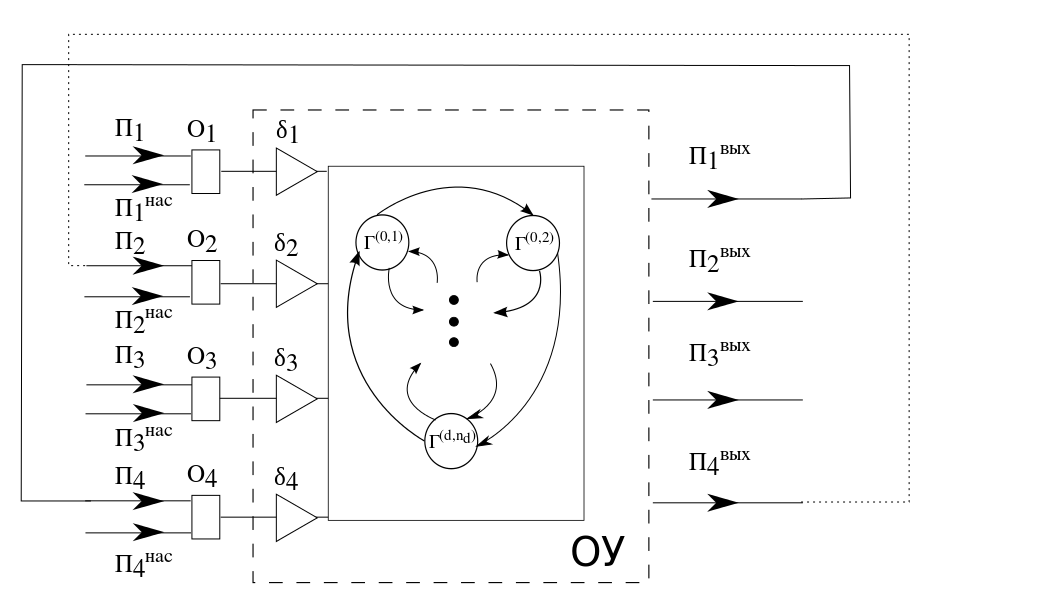
\includegraphics[scale=0.45]{Pictures/SystemScheme.png} 
\caption{Структурная схема системы обслуживания}
\label{SystemScheme}
\end{figure}
В систему,  осуществляющую операцию по обслуживанию одним обслуживающим устройством,  поступают потоки $\Pi_1$,  $\Pi_2$,  $\Pi_3$  и $\Pi_4$. Требования потока $\Pi_j$ приходят в соответствующую очередь $O_j$ неограниченного объема,  $j\in \{1,  2,  3,  4\}$. Дисциплина очереди $O_j$,  $j \in \{1,  2,  3\}$,  поддерживается при помощи устройства $\delta_j$ и имеет тип <<первым пришел~--- первым ушел>> (FIFO). Другими словами,  на обслуживание поступает требование,  пришедшее раньше остальных. Дисциплина очереди $O_4$ будет описана ниже. Будем предполагать,  что внешняя среда,  формирующая входные потоки $\Pi_1$ и $\Pi_3$,  имеет только одно состояние,  то есть вероятностная структура потоков не меняется с течением времени. 
Входящие потоки требований $\Pi_1$ и $\Pi_3$ являются неординарными пуассоновскими потоками,  то есть ординарными,  стационарными и без последействия потоками групп требований. Соответствующие простейшие потоки для $\Pi_1$ и $\Pi_3$ имеют интенсивности $\lambda_1$ и $\lambda_3$. При помощи следующей производящей функции зададим  распределение количества заявок в группе по потоку $\Pi_j$:
\begin{equation}
f_j(z) = \sum_{\nu=1}^{\infty} p_{\nu}^{(j)} z^{\nu},  \quad j\in \{1, 3\}.
\label{GeneratingFunc}
\end{equation}
Функцию $f_j(\cdot)$,  $j\in \{1, 3\}$,  будем предполагать аналитической при всех $z\in \mathbb{C}$ таких,  что $|z|\hm<(1+\varepsilon)$,  $\varepsilon>0$. Величина $p_{\nu}^{(j)}$ задает  вероятность того,  что по потоку $\Pi_j$ число требований в группе равно $\nu$. После обслуживания требования потока $\Pi_1$ повторно поступают в систему для обслуживания,  формируя при этом поток $\Pi_4$. Затем,  обслуженные требования потока $\Pi_4$ поступают на еще одно повторное обслуживание,  создавая при этом поток $\Pi_2$. Потоки $\Pi_2$ и $\Pi_3$ являются конфликтными,  что означает запрет на одновременное обслуживание требований этих потоков и,  следовательно,  исследование системы не может быть сведено к задаче с меньшим числом потоков. 

Обслуживающее устройство в каждый момент времени может находиться в одном из множества состояний $\Gamma=\{\Gamma^{(k, r)} \colon k=\overline{0, d}; r=\overline{1, n_k}\}$ с заданными натуральными числами $d$,  $n_0$,  $n_1$,  $\ldots$,  $n_d$. В каждом состоянии $\Gamma^{(k, r)}$ обслуживающее устройство находится в течение времени $T^{(k, r)}$. Выделим из множества $\Gamma$ подножества $\Gamma^{\mathrm{I}}$,  $\Gamma^{\mathrm{II}}$, 
$\Gamma^{\mathrm{III}}$ и $\Gamma^{\mathrm{IV}}$ следующим образом. В состоянии $\gamma \in \Gamma^{\mathrm{I}}$ обслуживаются только требования из очередей $O_1$,  $O_2$ и $O_4$.
В состоянии $\gamma \in \Gamma^{\mathrm{II}}$ обслуживаются только требования из очередей $O_2$ и $O_4$.
В состоянии $\gamma \in \Gamma^{\mathrm{III}}$ обслуживаются только требования из очередей $O_1$,  $O_3$ и $O_4$.
В состоянии $\gamma \in \Gamma^{\mathrm{IV}}$ обслуживаются только требования из очередей $O_3$ и $O_4$.
Тогда множество $\Gamma$ есть объединение $\Gamma = \Gamma^{\mathrm{I}} \cup \Gamma^{\mathrm{II}} \cup \Gamma^{\mathrm{III}} \cup\Gamma^{\mathrm{IV}}$ непересекающихся подмножеств. Также в дальнейшем нам понадобятся множества ${}^1\Gamma=\Gamma^{\mathrm{I}} \cup \Gamma^{\mathrm{III}}$,  
${}^2\Gamma=\Gamma^{\mathrm{I}} \cup \Gamma^{\mathrm{II}}$, 
${}^3\Gamma=\Gamma^{\mathrm{III}} \cup \Gamma^{\mathrm{IV}}$. 

Смена состояний обслуживающего устройства осуществляется по следующему правилу. Множество состояний $C_k = \{\Gamma^{(k, r)} \colon r=\overline{1, n_k}\}$ будем называть $k$-м циклом,  $k=\overline{1, d}$ (Рис. \ref{GraphScheme}). Состояние вида $\Gamma^{(0, r)}$ будем называть состоянием продления,  $r=\overline{1, n_0}$. Положим $r \oplus_k 1 = r+1$ для $r=\overline{1, n_k-1}$ и $r \oplus_k 1 = 1$ при $r=n_k$,  $k = \overline{0, d}$. В цикле $C_k$ выделим подмножества $C_k^{\mathrm{O}}$ выходных,  $C_k^{\mathrm{I}}$ входных и $C_k^{\mathrm{N}} = C_k \setminus (C_k^{\mathrm{O}} \cup C_k^{\mathrm{I}})$ нейтральных состояний. Тогда после состояния $\Gamma^{(k, r)} \hm\in C_k\setminus C_k^{\mathrm{O}}$ обслуживающее устройство переходит в состояние $\Gamma^{(k, r \oplus_k 1)}$ того же цикла $C_k$. При $\Gamma^{(k, r)}$,  принадлежащем множеству $C_k^{\mathrm{O}}$,  прибор переходит в состояние $\Gamma^{(k, r \oplus_k 1)}$,  если число требований в очереди $O_3$ в момент переключения больше заданного порога $L$. В противном случае,  то есть если число требований в очереди $O_3$ меньше либо равно $L$,  новое состояние прибора будет состоянием продления $\Gamma^{(0, r_1)}$,  где $r_1=h_1(\Gamma^{(k, r)})$ и $h_1(\cdot)$~--- заданное отображение множества $\bigcup\limits_{k=1}^d C_k^{\mathrm{O}}$ во множество $\{1, 2, \ldots,  n_0\}$. После состояния $\Gamma^{(0, r)}$ выбирается состояние того же вида $\Gamma^{(0, r_2)}$,  если число требований в очереди $O_3$ меньше или равно $L$,  где $r_2=h_2(r)$ и $h_2(\cdot)$~--- заданное отображение множества $\{1, 2,  \ldots,  n_0\}$ на себя; в противном случае включается входное состояние $\Gamma^{(k, r_3)} \in C_k^{\mathrm{I}}$,  где $\Gamma^{(k, r_3)}=h_3(r)$ и $h_3(\cdot)$~--- заданное отображение множества $\{1, 2,  \ldots,  n_0\}$ на множество  $\bigcup\limits_{k=1}^d C_k^{\mathrm{I}}$. Считается,  что все состояния продления $\Gamma^{(0, r)}$ принадлежат множеству ${}^2 \Gamma$,  а также верны соотношения $C_k^\mathrm{O}\subset {}^2 \Gamma$ и $C_k^\mathrm{I}\subset {}^3 \Gamma$. Также будем предполагать,  что все циклы имеют ровно одно входное и одно выходное состояние. И последним предположением является то,  что все вершины продления образуют один цикл,  то есть можем положить $h_2(r)=r\oplus_0 1$.

\begin{figure}[h]\centering
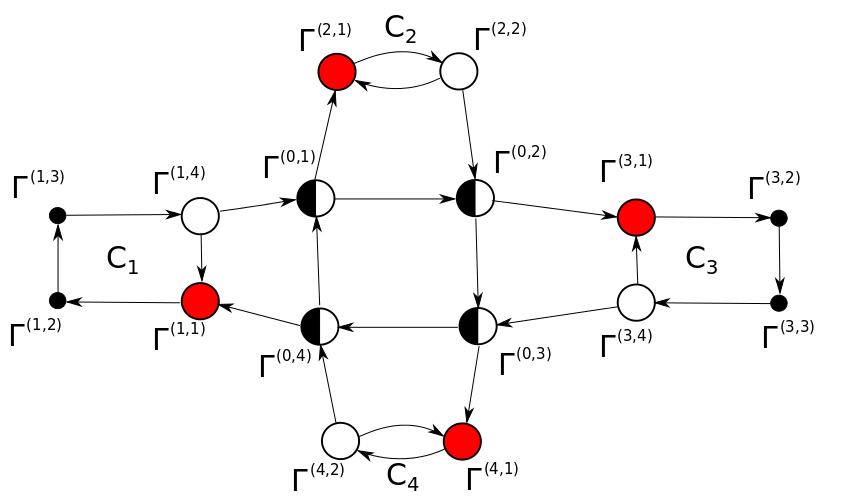
\includegraphics[scale=0.5]{Pictures/GraphScheme3.png} 
\caption{Класс графов переходов. Незакрашенные вершины являются выходными вершинами,  большие закрашенные вершины --- входные,  небольшие закрашенные --- нейтральные,  наполовину закрашенным вершинам соответствуют состояния продления}
\label{GraphScheme}
\end{figure}
%\subsection{Допустимые графы переходов состояний ОУ}

Таким образом,  смена состояний обслуживающего устройства задается соотношением:
\begin{equation}
h(\Gamma^{(k, r)}, y) = 
\begin{cases}
\Gamma^{(k, r \oplus_k 1)}, & \quad \text{если } (\Gamma^{(k, r)}\in C_k\setminus C_k^{\mathrm{O}}) \\
& \quad \text{или } (\Gamma^{(k, r)}\in C_k^{\mathrm{O}} \text{ и } y>L);\\
%\Gamma^{(k, r \oplus_k 1)}, & \quad \text{ если } \Gamma^{(k, r)}\in C_k^{\mathrm{O}} \text{ и } y>L;\\
\Gamma^{(0, h_1(\Gamma^{(k, r)}))}, & \quad \text{если } \Gamma^{(k, r)}\in C_k^{\mathrm{O}} \text{ и } y\leqslant L;\\
\Gamma^{(0, r \oplus_0 1)}, & \quad \text{если } k=0 \text{ и } y\leqslant L;\\
h_3(r), & \quad \text{если } k=0 \text{ и } y > L.
\end{cases}
\label{hLaw}
\end{equation}

Рассмотрим введеные обозначения для входных, выходных и нейтральных состояний на примере рис.~\ref{GraphScheme}. Входными состояниями обслуживающего устройства являются $\Gamma^{(1, 1)} \in C_1^{\mathrm{I}}$,  $\Gamma^{(2, 1)} \in C_2^{\mathrm{I}}$,  $\Gamma^{(3, 1)} \in C_3^{\mathrm{I}}$ и $\Gamma^{(4, 1)} \in C_4^{\mathrm{I}}$,  выходные состояния~--- $\Gamma^{(1, 4)} \in C_1^{\mathrm{O}}$,  $\Gamma^{(2, 2)} \in C_2^{\mathrm{O}}$,  $\Gamma^{(3, 4)} \in C_3^{\mathrm{O}}$ и $\Gamma^{(4, 2)} \in C_4^{\mathrm{O}}$,  нейтральные состояния~--- $\Gamma^{(1, 2)},  \Gamma^{(1, 3)} \in C_1^{\mathrm{N}}$ и $\Gamma^{(3, 2)},  \Gamma^{(3, 3)} \in C_3^{\mathrm{N}}$. Состояния продления на графе представлены вершинами $\Gamma^{(0, 1)}$,  $\Gamma^{(0, 2)}$,  $\Gamma^{(0, 3)}$ и $\Gamma^{(0, 4)}$. Далее,  отображение $h_1(\cdot)$ на графе задано таким образом,  что оно переводит,  например,  выходное состояние $\Gamma^{(1, 4)}$ в число $1$~--- номер состояния продления $\Gamma^{(0, 1)}$,  то есть $h_1(\Gamma^{(1, 4)})=1$. Аналогично,  например,  $h_2(1)=2$ и $h_2(3)=4$. Примером отображения $h_3(\cdot)$ является $h_3(2)=\Gamma^{(3, 1)}$.

Предполагается,  что длительности обслуживания различных требований могут  иметь различные законы распределения и, вообще говоря,  быть зависимыми,  поэтому вместо привычного способа,  состоящего в указании функции распределения длительности обслуживания произвольного требования,  будут использованы потоки насыщения. Потоками насыщения $\Pi^{\mathrm{\text{нас}}}_j$,  $j=\overline{1, 4}$,  назовем виртуальные выходные потоки при условии максимального использования ресурсов обслуживающего устройства,  а для $j=\overline{1, 3}$ еще и при условии максимальной загрузки соответствующих очередей.
Более конкретно,  поток насыщения $\Pi^{\mathrm{\text{нас}}}_j$,  $j=\overline{1, 3}$,  содержит неслучайное число $\ell(k, r, j)$ требований,  которые были обслужены в течение времени $T^{(k, r)}$,  если обслуживающее устройство находилось в состоянии $\Gamma^{(k, r)}$. Пусть $\mathbb{Z}_+$~--- множество целых неотрицательных чисел. Тогда,  при условии,  что в очереди $O_4$ находится $x \in \mathbb{Z}_+$ требований,  поток насыщения $\Pi^{\mathrm{\text{нас}}}_4$ определим как поток,  содержащий все $x$ требований.
%\subsection{Пример: тандем из двух перекрестков} 
Наконец,  при состоянии обслуживающего устройства $\Gamma^{(k, r)}$ каждое требование из очереди $O_4$ с вероятностью $p_{k, r}$ и независимо от других завершает обслуживание и отправляется в очередь $O_2$ потока~$\Pi_2$. С вероятностью $1-p_{k, r}$ требование очереди $O_4$ остается в ней до следующего такта. На следующем такте процесс повторяется.

В качестве наглядной физической интерпретации можно привести тандем из двух перекрестков (рис. \ref{crossroads}).
\begin{figure}[h]\centering
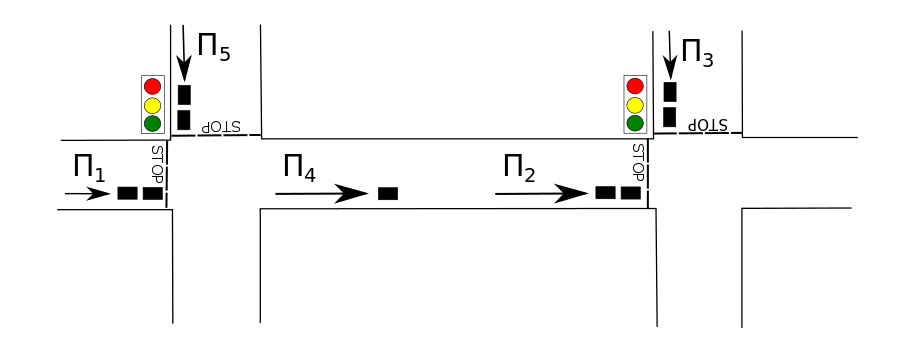
\includegraphics[scale=0.5]{Pictures/Crossroads.png} 
\caption{Пример: тандем перекрестков}
\label{crossroads}
\end{figure}
В качестве потоков требований,  формируемых внешней средой,  выступают потоки прибывающих на перекрестки машин: конфликтные потоки $\Pi_1$,  $\Pi_5$ на первом перекрестке,  а также поток $\Pi_3$ на втором. Каждая машина из потока $\Pi_1$,  проезжая первый перекресток,  становится в очередь $O_4$ потока $\Pi_4$ и затем с некой вероятностью ($p_{k, r}$ для состояния $\Gamma^{(k, r)}$ обслуживающего устройства) доезжает до следующего перекрестка,  или же не успевает это сделать и остается в очереди $O_4$ до следующего такта обслуживания. В случае,  если машина из очереди $O_4$ успевает доехать до второго перекрестка,  она становится в очередь $O_2$ и ждет своей очереди для его прохождения.

Предполагается,  что светофор на первом перекрестке имеет лишь два состояния $\{g_{1, 1}, g_{1, 2}\}$: в состоянии $g_{1, 1}$ машины потока $\Pi_1$ пропускаются фиксированное количество времени $\widetilde T^{(1, 1)}$ (<<зеленый>> свет для $\Pi_1$); в состоянии $g_{1, 2}$ --- простаивают в течение времени $\widetilde T^{(1, 2)}$ (<<красный>> свет для $\Pi_1$). Светофор на втором перекрестке обслуживает по алгоритму с продлением: дополнительно к состоянию обслуживания потока $\Pi_3$ (состояние $g_{2, 1}$),  также имеется два состояния обслуживания потока $\Pi_2$ (состояния $g_{2, 2}$,  $g_{2, 3}$). Первое из них включается всегда после завершения обслуживания потока $\Pi_3$,  а второе включается,  если после очередного такта обслуживания потока $\Pi_2$ длина очереди $O_3$ не превосходит уровня $L$.
Длительности пребывания светофора на втором перекрестке в каждом из состояний суть $\widetilde T^{(2, 1)}$,  $\widetilde T^{(2, 2)}$ и $\widetilde T^{(2, 3)}$.


Рассматривая тандем из двух перекрестков как единую систему массового обслуживания и предполагая наблюдение за ней только в (дискретные) моменты переключения состояния хотя бы одного из светофоров,  может быть показано,  что количество различных состояний у полученной системы конечно. Действительно,  положим,  например,  за состояние объединенной системы вектор $(g^{(1)},  g^{(2)},  s,  t)$,  где $g^{(1)}\in \{g_{1,  1},  g_{1,  2}\}$~--- состояние $1$--го перекрестка,  $g^{(2)}\in \{g_{2,  1},  g_{2,  2},  g_{2,  3}\}$~--- состояние $2$--го перекрестка,  $s \in \{0,  1,  2\}$~--- номер последнего сменившего состояние перекрестка (принимает значение $0$ в случае,  если сменили состояние оба перекрестка) и $t \in \{0,  1,  2,  \ldots,  T\}$~--- количество времени,  оставшееся у продолжающего обслуживание с прошлого такта перекрестка (принимает значение $0$,  если принимает значение $0$ величина $s$). Здесь $T$~--- максимальная длительность нахождения каждого из светофоров в одном состоянии. Тогда количество различных состояний не трудно посчитать и оно не будет превышать величины  $2\times 3 \times 3 \times T$.

В завершении построения примера отметим,  что при прохождении перекрестков машины предполагаются движущимися только в прямом направлении,  то есть перемешивания конфликтных потоков не допускается. Таким образом,  поток $\Pi_5$ не представляет интереса для дальнейшего исследования системы и может быть отброшен и,  следовательно,  построенный пример целиком удовлетворяет структурной схеме на рис.~\ref{SystemScheme}.

Теперь продемонстрируем на конкретном числовом примере выделение циклов и состояний продления. Пусть изменение состояний перекрестков и время пребывания (в секундах,  для определенности) в каждом из состояний задается графами на рис. \ref{SystemStates}.
\begin{figure}[h]\centering
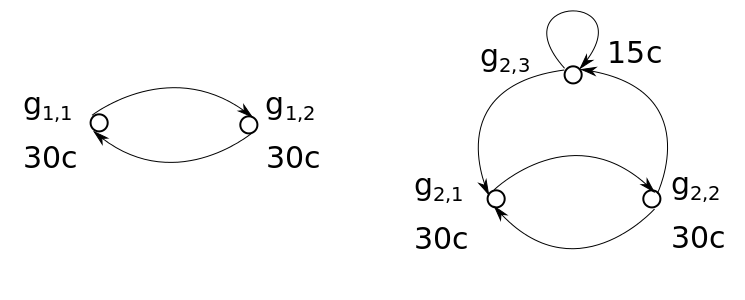
\includegraphics[scale=0.5]{Pictures/SystemStates.png} 
\caption{Числовой пример тандема перекрестков. Левый граф соответствует первому перекрестку,  правый~--- второму}
\label{SystemStates}
\end{figure}
За начальное состояние объединенной системы примем $\Gamma_0=(g_{1,  1},  g_{2,  1},  0,  0)$,  то есть первый перекресток находится в состоянии $g_{1, 1}$,  второй~--- в состоянии $g_{2,  1}$,  и оба только начали свою работу в своем состоянии (этот факт моделируется равенствами $s=0$ и $t=0$). Следующая смена состояний случится у обоих перекрестков одновременно и приведет к следующему состоянию $(g_{1,  2},  g_{2,  2},  0,  0)$. Далее смена состояний произойдет также у первого и второго перекрестков,  однако второй перекресток может перейти как в состояние $g_{2,  1}$,  так и в состояние продления $g_{2,  3}$. Таким образом,  следущим состоянием тандема будет либо опять $(g_{1,  1},  g_{2,  1},  0,  0)$,  либо $(g_{1,  1},  g_{2,  3},  0,  0)$. Продолжая рассуждения аналогичным образом,  получим следущий список всех возможных состояний системы:
\begin{align*}
(g_{1,  1},  g_{2,  1},  0,  0)&=\Gamma^{(1,  1)} ,  & \quad (g_{1,  2},  g_{2,  2},  0,  0)&=\Gamma^{(1,  2)} ,  & \quad (g_{1,  1},  g_{2,  3},  0,  0)&=\Gamma^{(0,  1)},   \\
(g_{1,  1},  g_{2,  3},  15,  2)&=\Gamma^{(0,  2)} ,  & \quad (g_{1,  2},  g_{2,  3},  0,  0)&=\Gamma^{(0,  3)} ,  & \quad (g_{1,  2},  g_{2,  3},  15,  2)&=\Gamma^{(0,  4)},   \\
(g_{1,  2},  g_{2,  1},  15,  2)&=\Gamma^{(4,  1)} ,  & \quad (g_{1,  1},  g_{2,  1},  15,  1)&=\Gamma^{(4,  2)} ,  & \quad (g_{1,  1},  g_{2,  2},  15,  2)&=\Gamma^{(4,  3)},   \\
(g_{1,  2},  g_{2,  2},  15,  1)&=\Gamma^{(4,  4)} ,  & \quad (g_{1,  2},  g_{2,  3},  15,  2)&=\Gamma^{(0,  5)} ,  & \quad (g_{1,  2},  g_{2,  1},  0,  0)&=\Gamma^{(3,  1)},   \\
(g_{1,  1},  g_{2,  2},  0,  0)&=\Gamma^{(3,  2)} ,  & \quad (g_{1,   1},  g_{2,  1},  15,  2)&=\Gamma^{(2,  1)} ,  & \quad (g_{1,  2},  g_{2,  1},  15,  1)&=\Gamma^{(2,  2)},   \\
(g_{1,  2},  g_{2,  2},  15,  2)&=\Gamma^{(2,  3)} ,  & \quad (g_{1,  1},  g_{2,  2},  15,  1)&=\Gamma^{(2,  4)}. & &
\end{align*}
В соответствии с приведенными выше обозначениями,   множества $C_1$,  $C_2$,  $C_3$,  $C_4$,  а также множество состояний продления строятся однозначным образом. Множествами входных состояний будут $C_1^{\mathrm{I}}=\{\Gamma^{(1,  1)}\}$,  $C_2^{\mathrm{I}}=\{\Gamma^{(2,  1)}\}$,  $C_3^{\mathrm{I}}=\{\Gamma^{(3,  1)}\}$ и $C_4^{\mathrm{I}}=\{\Gamma^{(4,  1)}\}$. Множествами выходных состояний будут $C_1^{\mathrm{O}}=\{\Gamma^{(1,  2)}\}$,  $C_2^{\mathrm{O}}=\{\Gamma^{(2,  4)}\}$,  $C_3^{\mathrm{O}}=\{\Gamma^{(3,  2)}\}$ и $C_4^{\mathrm{O}}=\{\Gamma^{(4,  4)}\}$. Функции $h_1(\cdot)$,  $h_2(\cdot)$ и $h_3(\cdot)$ задаются поточечно:
\begin{equation*}
h_1(\Gamma^{(1,  2)})=1,  \quad h_1(\Gamma^{(2,  4)})=2,  \quad h_1(\Gamma^{(3,   2)})=3,  \quad h_1(\Gamma^{(4,  4)})=5, 
\end{equation*}
\begin{equation*}
h_2(1)=2,  \quad h_2(2)=3,  \quad h_2(3)=4 \quad h_2(4)=1,  \quad h_2(5)=1, 
\end{equation*}
\begin{equation*}
h_3(1)=\Gamma^{(2, 1)},  \quad h_3(2)=\Gamma^{(3, 1)},  \quad h_3(3)=\Gamma^{(4, 1)} \quad h_3(4)=\Gamma^{(1, 1)},  \quad h_3(5)=\Gamma^{(1, 1)}.
\end{equation*}
Этим завершается построение числового примера.

\section{Представление рассматриваемой системы обслуживания в виде абстрактной управляющей системы Ляпунова--Яблонского}
Описанная в предыдущем разделе на содержательном уровне система массового обслуживания должна рассматриваться как абстрактная управляющая система обслуживания (см. \cite{Zorin:2011:2}). Схема управляющей системы представлена на рис. \ref{SystemScheme}. Схема состоит из следующих блоков: 1)~входные полюса первого типа~--- входные потоки $\Pi_1$,  $\Pi_2$,  $\Pi_3$,  $\Pi_4$; 2)~входные полюса второго типа~--- потоки насыщения $\Pi_1^{\mathrm{\text{нас}}}$,  $\Pi_2^{\mathrm{\text{нас}}}$,  $\Pi_3^{\mathrm{\text{нас}}}$,  $\Pi_4^{\mathrm{\text{нас}}}$; 3)~выходные полюса $\Pi_1^{\mathrm{\text{вых}}}$,  $\Pi_2^{\mathrm{\text{вых}}}$,  $\Pi_3^{\mathrm{\text{вых}}}$,  $\Pi_4^{\mathrm{\text{вых}}}$; 4)~внутренняя память~--- обслуживающее устройство (ОУ);  5)~устройство по переработке информации внутренней памяти~--- граф смены состояний;  6)~внешняя память~--- очереди $O_1$,  $O_2$,  $O_3$,  $O_4$; 7)~устройство по переработкe информации внешней памяти~--- устройства по поддержанию дисциплины очереди $\delta_1$,  $\delta_2$,  $\delta_3$,  $\delta_4$; 8) внешняя среда с одним состоянием. Координатой блока является номер этого блока на схеме.

Зададим информацию о блоках с помощью следующих случайных величин и элементов,  указав,  в том числе,  множества их возможных значений. В качестве дискретной временной шкалы выберем последовательность $\tau_0=0$,  $\tau_1$,  $\tau_2$,  $\ldots$ моментов смены состояния обслуживающего устройства. Обозначим:
\begin{itemize}
\item $\Gamma_i$,  $i\geqslant 1$,  из множества $\Gamma$~--- состояние обслуживающего устройства в течение времени $\left(\tau_{i-1};\tau_i\right]$ и $\Gamma_0\in \Gamma$~--- в момент времени $\tau_0$;
\item количество $\varkappa_{j, i} \in \mathbb{Z}_+ $,  $i\geqslant 0$,  требований в очереди $O_j$ в момент времени $\tau_i$;
\item количество $\eta_{j, i} \in \mathbb{Z}_+$,  $i\geqslant 0$,  требований,  поступивших в очередь $O_j$ по потоку $\Pi_j$ в течение времени $\left(\tau_{i};\tau_{i+1}\right]$;
\item количество $\xi_{j, i} \in \mathbb{Z}_+$,  $i\geqslant 0$,  требований по потоку насыщения $\Pi^{\mathrm{\text{нас}}}_j$ в течение времени $\left(\tau_{i};\tau_{i+1}\right]$;
\item количество $\overline{\xi}_{j, i}\in \mathbb{Z}_+$,  $i\geqslant 0$,  реально обслуженных требований по потоку $\Pi_j$ в течение времени $\left(\tau_{i};\tau_{i+1}\right]$; $j=\overline{1, 4}$.
\end{itemize}
Закон изменения состояния обслуживающего устройства будем предполагать заданным соотношением 
\begin{equation}
\Gamma_{i+1}=h(\Gamma_i,  \varkappa_{3, i}), 
\label{gammaFunc}
\end{equation}
где отображение $h(\cdot,  \cdot)$ определено в \eqref{hLaw}.
Для определения длительности $T_{i+1}$ состояния обслуживающего устройства в течение времени $\left(\tau_{i};\tau_{i+1}\right]$ удобно ввести функцию $h_T(\cdot,  \cdot)$:
\begin{equation*}
T_{i+1}=h_T(\Gamma_i,  \varkappa_{3,  i})= T^{(k,  r)}, \quad  \text{ где $k$ и $r$ таковы,  что } \Gamma^{(k,  r)}=\Gamma_{i+1}=h(\Gamma_i, \varkappa_{3,  i}).
%\label{timeLaw}
\end{equation*}
Функциональная зависимость
\begin{equation}
\overline{\xi}_{j,  i}=\min\{\varkappa_{j,  i}+\eta_{j,  i},  \xi_{j,  i}\},  \quad j \in \{1,  2,  3\}, 
\label{saturationEq}
\end{equation}
между величиной $\overline{\xi}_{j, i}$ и величинами $\varkappa_{j, i}$,  $\eta_{j, i}$,  $\xi_{j, i}$ реализует стратегию механизма обслуживания требований. Далее,  поскольку 
\begin{equation*}
\varkappa_{j,  i+1}=\varkappa_{j,  i}+\eta_{j,  i}-\overline{\xi}_{j,  i},  \quad  j \in \{1,  2,  3\}, 
\end{equation*}
то из выражения \eqref{saturationEq} следует соотношение
\begin{equation}
\varkappa_{j,  i+1}=\max\{{0,  \varkappa_{j,  i}+\eta_{j,  i}-\xi_{j,  i}}\},  \quad j \in \{1,  2,  3\}.
\label{queuesFunc}
\end{equation}
Из формулировки поставленной задачи (см. также структурную схему на рис.~\ref{SystemScheme}) следуют соотношения для потока $\Pi_4$:
\begin{equation}
\eta_{4, i} = \min\{\xi_{1, i},  \varkappa_{1, i}+\eta_{1, i}\},  \quad \varkappa_{4, i+1}=\varkappa_{4, i}+\eta_{4, i}-\eta_{2, i},  \quad \xi_{4, i} = \varkappa_{4, i}.
\label{FourthFunc}
\end{equation}

Нелокальное описание входных потоков и потоков насыщения состоит в указании некоторых свойств условных распределений выделенных дискретных компонент $\eta_i=(\eta_{1,  i},  \eta_{2,  i},  \eta_{3,  i},  \eta_{4,  i})$ и $\xi_i \hm{=} (\xi_{1,  i},  \xi_{2,  i},  \xi_{3,  i},  \xi_{4,  i})$ маркированных точечных процессов  $\{(\tau_i,  \nu_i,  \eta_i); i\geqslant 0\}$ и $\{(\tau_i,  \nu_i,  \xi_i); i\geqslant 0\}$ при фиксированных значениях метки $\nu_i \hm= (\Gamma_i; \varkappa_i)$,  где $\varkappa_i=(\varkappa_{1,  i},  \varkappa_{2,  i},  \varkappa_{3,  i},  \varkappa_{4,  i})$. 
Введем функции $\varphi_1(\cdot,  \cdot)$ и $\varphi_3(\cdot,  \cdot)$ из разложений 
\begin{equation*}
\sum_{\nu=0}^{\infty} z^\nu\varphi_j(\nu,  t) = \exp\{\lambda_j t (f_j(z)-1)\}, 
\end{equation*}
где $f_j(z)$ определены выражением \eqref{GeneratingFunc},  $j \in \{1, 3\}$. Функция $\varphi_j(\nu,  t)$ по своему смыслу есть вероятность поступления $\nu=0$,  $1$,  $\ldots$ требований по потоку $\Pi_j$ за промежуток времени от $0$ до $t \geqslant 0$. Положим $\varphi_j(\nu, t)$ равной нулю при $\nu < 0$. Функцию $\psi(\cdot,  \cdot,  \cdot)$ зададим формулой
\begin{equation*}
\psi(k;y, u)=C_y^k u^k (1-u)^{y-k}.	
\end{equation*}
По своему смыслу $\psi(k; y,  u)$ есть вероятность поступления $k$ требований по потоку $\Pi_2$ при условии,  что очередь $O_4$ содержит $y$ требований и обслуживающее устройство находится в состоянии $\Gamma^{(k,  r)}$,  так что $u=p_{k,  r}$. При нарушении условия $ 0\leqslant k \leqslant y$ положим $\psi(k; y,  u)$ равной нулю.

Пусть $a=(a_1,  a_2,  a_3,  a_4) \in \mathbb{Z}_+^4$ и $x=(x_1,  x_2,  x_3,  x_4) \in \mathbb{Z}_+^4$. Тогда из постановки задачи на содержательном уровне следует,  что при фиксированном значении метки $\nu_i=(\Gamma^{(k,  r)}; x)$ вероятность $\varphi(a,  k,  r,  x)$ одновременного выполнения равенств $\eta_{1,  i}=a_1$,  $\eta_{2,  i}=a_2$,  $\eta_{3,  i}=a_3$,  $\eta_{4,  i}=a_4$ есть 
\begin{equation}
\varphi_1(a_1,  h_T(\Gamma^{(k,  r)},  x_3)) \times \psi(a_2,  x_4,  p_{\tilde{k},  \tilde{r}}) \times \varphi_3(a_3,  h_T(\Gamma^{(k,  r)},  x_3))
\times \delta_{a_4,  \min{\{\ell(\tilde{k},  \tilde{r},  1),  x_1+a_1}\}}, 
\label{conditionProbOne}
\end{equation}
где $\tilde{k}$ и $\tilde{r}$ таковы,  что $\Gamma^{(\tilde{k},  \tilde{r})}=h(\Gamma^{(k,  r)},  x_3)$ и $\delta_{i,  j}$ есть символ Кронекера:
%\begin{equation*}
$$
\delta_{i,  j}=
\begin{cases} 
1, & \quad \text{ если $i=j$, }\\
0, & \quad \text{ если $i\neq j$.}
\end{cases}
$$%\end{equation*}
Пусть $b=(b_1,  b_2,  b_3,  b_4) \in \mathbb{Z}_+^4$. Из содержательной постановки задачи также следует,  что вероятность $\zeta(b,  k,  r,  x)$ одновременного выполнения равенств $\xi_{1,  i}\hm=b_1$,  $\xi_{2,  i}=b_2$,  $\xi_{3,  i}=b_3$,  $\xi_{4,  i}=b_4$ при фиксированном значении $(\Gamma^{(k,  r)}; x)$ метки $\nu_i$ есть
\begin{equation}
\delta_{b_1,  \ell(\tilde{k},  \tilde{r},  1)} \times \delta_{b_2,  \ell(\tilde{k},  \tilde{r},  2)} \times 
\delta_{b_3,  \ell(\tilde{k},  \tilde{r},  3)} \times \delta_{b_4,  x_4}.
\label{conditionProbTwo}
\end{equation}
Из формулы \eqref{conditionProbTwo} следует для $j\in \{1,  2,  3\}$,  что вероятность события $\xi_{j,  i}=0$ равна $1$ в случае $h(\Gamma^{(k,  r)},  x_3)\notin {}^j\Gamma$ и что вероятность события $\xi_{j, i}=\ell(\tilde{k},  \tilde{r},  j)$ равна $1$,  если $\Gamma^{(\tilde{k},  \tilde{r})}=h(\Gamma^{(k,  r)},  x_3)\in {}^j\Gamma$.


Содержательный смысл следующей теоремы состоит в том,  что сформулированные выше функциональные связи и вероятностные свойства введенных объектов непротиворечивы и могут быть реализованы на некотором вероятностном пространстве.
%Построим теперь 	вероятностное пространство $(\Omega,  {\mathcal F},  \Pr(\cdot))$,  чтобы можно было рассматривать введеные величины как случайные величины на этом пространстве. А именно,  докажем следующую теорему.

\begin{theorem}
Пусть $\gamma_0=\Gamma^{(k_0,  r_0)}\in \Gamma$ и $x^0=(x_{1,  0},  x_{2,  0},   x_{3,  0},  x_{4,  0})\in \mathbb{Z}_+^4$ фиксированы.
Тогда существует вероятностное пространство $(\Omega,   {\mathcal F},   \Pr(\cdot))$ и заданные на нем случайные величины $\eta_{j,  i}=\eta_{j,  i}(\omega)$,   $\xi_{j,  i}=\xi_{j,  i}(\omega)$,   	 $\varkappa_{j,  i}=\varkappa_{j,  i}(\omega)$ и случайные элементы $\Gamma_i=\Gamma_i(\omega)$,   $i\geqslant 0$,   $j\in \overline{1,  4}$,   такие,   что 1) имеют место равенства $\Gamma_0(\omega) = \gamma_0$ и $\varkappa_0(\omega)=x^0$; 2) выполняются соотношения \eqref{gammaFunc},   \eqref{queuesFunc},   \eqref{FourthFunc}; 3) для любых  $a\in \mathbb{Z}_+^4$,   $b\in \mathbb{Z}_+^4$ и любых $x^t=(x_{1,  t},  x_{2,  t},  x_{3,  t},  x_{4,  t}) \in \mathbb{Z}_+^4$,   $\Gamma^{(k_t,  r_t)} \in \Gamma$,   $t = 1,   2,   \ldots$,   таких,   что $\Pr\Bigl(\bigcap\limits_{t=0}^{i}\{\omega\colon \Gamma_t=\Gamma^{(k_t,  r_t)},   \varkappa_t=x^t\}\Bigr)>0$,   условное распределение векторов $\eta_i$ и $\xi_i$,   $i \geqslant 0$,    имеет вид
\begin{multline}
\Pr \Bigl(\{ \omega \colon \eta_i = a,   \xi_i=b\} \,\,\Big
|\bigcap_{t=0}^{i}\{\omega\colon \Gamma_t=\Gamma^{(k_t,  r_t)},   \varkappa_t=x^t\}\Bigr)= \\=
\varphi(a,  k_i,  r_i,  x^i)\times \zeta(b,  k_i,  r_i,  x^i),  
\label{ProbablititiesToProve}
\end{multline}
где функции $\varphi(\cdot,   \cdot,   \cdot,   \cdot)$ и $\zeta(\cdot,   \cdot,   \cdot,   \cdot)$ определяются формулами \eqref{conditionProbOne} и \eqref{conditionProbTwo}.

\label{myTheorem}
\end{theorem}
\begin{proof}
Для построения вероятностного пространства $(\Omega,   {\mathcal F},   \Pr(\cdot))$ воспользуемся теоремой Ионеску Тулча (см. \cite{Shiryaev},   c. 348). 

Введем последовательность измеримых пространств $(\Omega_0,   {\mathcal F}_0)$,   $(\Omega_1,   {\mathcal F}_1)$,   $\ldots$,   где $\Omega_i\hm=\mathbb{Z}_+^3$,   $\omega_i=(\omega_{1,  i},  \omega_{2,  i},  \omega_{3,  i}) \hm\in \Omega_i$,   а $\sigma$-алгебра ${\mathcal F}_i=2^{\Omega_i}$  есть множество всех подмножеств множества $\Omega_i$. 
Пусть $\Gamma^{(\tilde{k},  \tilde{r})}=h(\Gamma^{(k_0,  r_0)},  x_{3,  0})$.
Зададим на измеримом пространстве $(\Omega_0,   {\mathcal F}_0)$ вероятностную меру $P_0(\cdot)$ ее значениями на одноточечных множествах:
\begin{multline}
P_0(\{(a_1,  a_2,  a_3)\})=\\=\varphi_1(a_1,  h_T(\Gamma^{(k_0,  r_0)})) \times \psi(a_2,  x_{2,  0},   p_{\tilde{k},  \tilde{r}}) \times \varphi_3(a_3,  h_T(\Gamma^{(k_0,  r_0)})).
\label{probabilitiesOne}
\end{multline}

Для $j\in \{1,  2,  3\}$ определим величины
\begin{equation}
\tilde{\Gamma}_0(\omega_0)=\gamma_0,  \quad \tilde{\varkappa}_{j,  0}(\omega_0)=x_{j,  0},   \quad \tilde{\xi}_{j,  0}(\omega_0)=l(\tilde{k},  \tilde{r},  j),   \quad \tilde{\eta}_{j,  0}(\omega_0)=\omega_{j,  0},  
\label{startRekOne}
\end{equation}
и
\begin{equation}
\begin{aligned}
 &\tilde{\varkappa}_{4,  0}(\omega_0)=x_{4,  0},   \quad \tilde{\xi}_{4,  0}(\omega_0)=x_{4,  0},  \\
&\tilde{\eta}_{4,  0}(\omega_0)=\min\{\tilde{\xi}_{1,  0}(\omega_0),   \tilde{\varkappa}_{1,  0}(\omega_0)+\tilde{\eta}_{1,  0}(\omega_0)\}
\end{aligned}
\label{startRekTwo}
\end{equation}

Теперь предположим,   что заданы вероятностные меры $$
P_i(\omega_0\hm{},  \omega_1, \hm{} \ldots \hm{},  \omega_{i-1};\cdot)
$$
на измеримых пространствах $(\Omega_i,  {\mathcal F}_i)$,  $i=\overline{0,  n}$,  
и 
% определеныслучайные величины $\tilde{\Gamma}_i$,  $\tilde{\varkappa}_{j, i}$,  $\tilde{\xi}_{j, i}$,  $\tilde{\eta}_{j, i}$,  ч,  и 
фиксирован набор $(\omega_0,  \omega_1,  \hm\ldots,  \omega_{n})$. Положим для $j\in \{1,  2,  3\}$  и $i=\overline{0,  n}$
\begin{equation}
\tilde{\Gamma}_{i+1}=\Gamma^{(k^*,  r^*)}=h(\tilde{\Gamma}_{i},  \tilde{\varkappa}_{3,  i}),   \quad \tilde{\varkappa}_{j,  i+1}=\max\{ 0,  \tilde{\varkappa}_{j,  i}+\tilde{\eta}_{j,  i} -\tilde{\xi}_{j,  i}\},  
\label{NextRekOne}
\end{equation}
\begin{equation}
\tilde{\varkappa}_{4,  i+1}=\tilde{\varkappa}_{4,  i}+\tilde{\eta}_{4,  i}-\tilde{\eta}_{2,  i},   \quad \tilde{\xi}_{j,  i+1}=l(k^*,  r^*,  j),  \quad \tilde{\eta}_{j,  i+1}=\omega_{j,  i+1},
\label{NextRekTwo}
\end{equation}
\begin{equation}
\tilde{\eta}_{4,  i+1}=\min\{\tilde{\xi}_{1,  i+1},   \tilde{\varkappa}_{1,  i+1}+\tilde{\eta}_{1,  i+1}\},   \quad \tilde{\xi}_{4,  i+1}=\tilde{\varkappa}_{4,  i+1}.
\label{NextRekThree}
\end{equation}
Заметим,   что значения $\tilde{\Gamma}_{i}$,   $\tilde\xi_{j,  i}$,   $\tilde\eta_{j,  i}$,   $\tilde\varkappa_{j,  i}$,   найденные по формулам \eqref{NextRekOne}--\eqref{NextRekThree} по наборам $(\omega_0,   \omega_1,  \ldots,   \omega_n)$ и $(\omega_0,   \omega_1,  \ldots,   \omega_i)$,   $n\geqslant i$,   совпадают.
Определим на измеримом пространстве $(\Omega_{n+1},   {\mathcal F}_{n+1})$ вероятностную меру  $P_{n+1}(\omega_0,   \omega_1,   \hm\ldots,   \omega_n;\cdot)$
ее значениями на одноточечных множествах $\{(a_1,  a_2,  a_3)\}$,   $(a_1,  a_2,  a_3)\hm\in {\mathbb Z}_+^3$:
\begin{multline}
P(\omega_0,  \omega_1,  \ldots,  \omega_n;\{(a_1,  a_2,  a_3)\}) = \\
= \varphi_1(a_1,  h_T(\tilde{\Gamma}_n,  \tilde{\varkappa}_{3,  n})) \times \psi(a_2,  \tilde{\varkappa}_{4,  n},   p_{k^*,  r^*}) \times \varphi_3(a_3,  h_T(\tilde{\Gamma}_n,  \tilde{\varkappa}_{3,  n})).
\label{probabilitiesTwo}
\end{multline}

%причем для любого множества $B\in {\mathcal F}_i$ функции $P(\omega_0, \omega_1, \hm\ldots,   \omega_{i-1};B)$ должны быть измеримыми функциями от $(\omega_0,  \omega_1,  \ldots,  \omega_{i-1})$. 


Тогда (в соответствии с теоремой Ионеску Тулчи) для декартова произведения $\Omega=\prod\limits_{i=0}^{\infty}\Omega_i$ пространств элементарных исходов и произведения $\sigma$-алгебр ${\mathcal F}=\bigotimes\limits_{i=0}^{\infty} {\mathcal F}_i$ на $(\Omega,  {\mathcal F})$ будет существовать единственная вероятностная мера $\Pr(\cdot)$ такая,   что для любого $i \geqslant 0$ верно равенство
\begin{equation}
\Pr(\{\omega \colon \omega_0 \in A_0,   \omega_1 \in A_1,   \ldots,  \omega_i\in A_i\})= P_i(A_0 \times A_1 \times \ldots \times A_i), 
\label{ProbabilitiesGeneral}
\end{equation}
где 
\begin{multline}
 P_i(A_0 \times A_1 \times \ldots \times A_i) =\\ = \int_{A_0} P_0(d \omega_0) \int_{A_1} P_1(\omega_0;d \omega_1) \ldots \int_{A_i} P_i(\omega_0,  \omega_1,  \ldots,  \omega_{i-1}; d \omega_i), 
\label{ProbabilitiesGeneralOne}
\end{multline}
для любого $A_i$ из ${\mathcal F}_i$. Итак,  вероятностное пространство $(\Omega,  {\mathcal F},  \Pr(\cdot))$ построено. 

Теперь введем на пространстве $(\Omega,  {\mathcal F},  \Pr(\cdot))$ следующие случайные величины и элементы,   $i \geqslant 0$,   $j =\overline{1,  4}$:
\begin{equation*}
    \Gamma_i(\omega) = \tilde{\Gamma}_i,   \quad \varkappa_{j,  i}(\omega) = \tilde{\varkappa}_{j,  i},  \quad
    \xi_{j,  i}(\omega) = \tilde{\xi}_{j,  i},   \quad \eta_{j,  i}(\omega) = \tilde{\eta}_{j,  i}.
\end{equation*}
и докажем,   что они  удовлетворяют условиям теоремы. Для сокращения записи зависимость от $\omega$ в обозначении случайных элементов и случайных величин далее будем опускать. Из формулы \eqref{NextRekOne} следует,   что случайные элементы $\Gamma_i$ удовлетворяют соотношению \eqref{gammaFunc},  а случайные величины $\varkappa_{j,  i}$ для $j\in \{1,   2,   3\}$ удовлетворяют соотношению \eqref{queuesFunc}. Из формулы \eqref{NextRekTwo} заключаем,  что $\varkappa_{4,  i}$ удовлетворяет соотношению $\eqref{FourthFunc}$. Далее,  из условий \eqref{startRekTwo} и \eqref{NextRekThree} следует справедливость соотношений \eqref{FourthFunc} для величин $\eta_{4,  i}$ и $\xi_{4,  i}$. 

Перейдем к доказательству равенства \eqref{ProbablititiesToProve}. Для этого найдем явное выражение для условной вероятности 
$$
\Pr (\{ \omega \colon \eta_i = a,  \xi_i=b\} | \bigcap_{t=0}^{i}\{\omega\colon \Gamma_t=\Gamma^{(k_t,  r_t)},   \varkappa_t=x^t\}).
$$
Пусть $\Gamma^{(\tilde{k}_i,  \tilde{r}_i)}=h(\Gamma^{(k_i,  r_i)},  x^i)$. Запишем по определению условной вероятности,   предполагая,   что $\Pr\Bigl(\bigcap\limits_{t=0}^{i}\{\omega\colon \Gamma_t=\Gamma^{(k_t,  r_t)},   \varkappa_t=x^t\}\Bigr)>0$:
\begin{multline}
\Pr \biggl(\left\{ \omega \colon \eta_i = a,   \xi_i=b\right\}  \bigg| \bigcap_{t=0}^{i}\left\{\omega\colon \Gamma_t=\Gamma^{(k_t,  r_t)},   \varkappa_t=x^t\right\}\biggr) = \\
=\Pr\biggl(\{ \omega \colon \eta_i = a,   \xi_i=b \} \cap \bigcap_{t=0}^{i}\{\omega\colon \Gamma_t=\Gamma^{(k_t,  r_t)},   \varkappa_t=x^t\}\biggr) \times \\
\times
\biggl(\Pr\biggl( \bigcap_{t=0}^{i}\{\omega\colon \Gamma_t=\Gamma^{(k_t,  r_t)},   \varkappa_t=x^t\}\biggr)\biggr)^{-1}.
\label{Construction:1}
\end{multline}
Далее из соотношений \eqref{ProbabilitiesGeneral},   \eqref{ProbabilitiesGeneralOne} и того факта,   что значения $\Gamma_i$ и $\varkappa_{i}$ зависят только от $\omega_0$,  $\omega_1$ ,  $\ldots$,  $\omega_{i-1}$,   но не от $\omega_i$,   (этот факт следует из формул \eqref{startRekOne}~--~\eqref{NextRekTwo}),   получим выражение для второго сомножителя последнего выражения
\begin{multline}
\Pr\biggl( \bigcap_{t=0}^{i}\{\omega\colon \Gamma_t=\Gamma^{(k_t,  r_t)},   \varkappa_t=x^t\}\biggr)=\\
=\sum_{\substack{\omega_0,   \omega_1,  \ldots,   \omega_{i-1} \colon \\ \Gamma_t=\Gamma^{(k_t,  r_t)},  \,   \varkappa_t=x^t,  \\ t=\overline{0,  i}}} P_0(\omega_0)\times P_1(\omega_0;\{\omega_1\})\times\ldots\times P_{i-1}(\omega_0,  \omega_1,  \ldots,   \omega_{i-2};\{\omega_{i-1}\}).
\label{Construction:2}
\end{multline}
%Здесь мы положили $A_t(\omega_0,  \omega_1,  \ldots,  \omega_{t-1})=\{\omega_t \colon \Gamma_t=\Gamma^{(k_t,  r_t)},   \varkappa_t=x^t\}$,   $t=\overline{0,  i}$.
Преобразуем множество 
$$
\{\omega\colon \eta_i = a,   \xi_i=b \} \cap \{\omega\colon\Gamma_i=\Gamma^{(k_i,  r_i)},   \varkappa_i=x^i\},
$$
учитывая соотношения \eqref{startRekOne}~--~\eqref{NextRekThree}:
\begin{multline*}
\Bigl\{\omega\colon \eta_i = a,  \xi_i=b \Bigr\} \cap \Bigl\{\omega\colon\Gamma_i=\Gamma^{(k_i,  r_i)},   \varkappa_i=x^i\Bigr\} = \Bigl\{\omega\colon\Gamma_i=\Gamma^{(k_i,  r_i)},   \varkappa_i=x^i\Bigr\} \cap\\
\cap \Bigl\{\omega\colon \eta_{j,  i} = a_j,   j=\overline{1,  3}\Bigr\} \cap \Bigl\{\omega\colon \xi_{j,  i} = b_j,   j=\overline{1,  3}\Bigr\} \cap \Bigl\{ \omega\colon\xi_{4,  i} = b_4 \Bigr\} \cap \\ \cap \Bigl\{\omega\colon \eta_{4,  i} = a_4 \Bigr\} 
= \Bigl\{\omega\colon\Gamma_i=\Gamma^{(k_i,  r_i)},   \varkappa_i=x^i\Bigr\} \cap \\ \cap \Bigl\{\omega\colon \omega_{j,  i} = a_j,   j= \overline{1,  3}\Bigr\} 
\cap \Bigl\{\omega\colon b_j=\ell(\tilde{k}_i,  \tilde{r}_i,  j),   j=\overline{1,  3}\Bigr\} \cap \\ 
\cap \Bigl\{ \omega\colon b_4 = x_{4,  i} \Bigr\} \cap  \Bigl\{\omega\colon a_4=\min\Bigl\{\ell(\tilde{k}_i,  \tilde{r}_i,  1),   x_{1,  i}+a_1\Bigr\} \Bigr\}. 
\end{multline*}
Тогда для первого множителя из правой части выражения \eqref{Construction:1} имеем:
\begin{multline}
\Pr\biggl(\Bigl\{ \omega \colon \eta_i = a,   \xi_i=b \Bigr\} \cap \bigcap_{t=0}^{i}\Bigl\{\omega\colon \Gamma_t=\Gamma^{(k_t,  r_t)},   \varkappa_t=x^t\Bigr\}\biggr)=\displaybreak[0]\\
= \Pr\biggl(\Bigl\{\omega\colon \eta_i = a,   \xi_i=b \Bigr\} \cap \Bigl\{\omega\colon\Gamma_i=\Gamma^{(k_i,  r_i)},   \varkappa_i=x^i\Bigr\} \cap \\ \cap \bigcap_{t=0}^{i-1}\{\omega\colon \Gamma_t=\Gamma^{(k_t,  r_t)},   \varkappa_t=x^t\}\biggr)\displaybreak[0]
= \delta_{b_4,  x_{4,  i}} \times \delta_{a_4,  \min\{\ell(\tilde{k}_i,  \tilde{r}_i,  1),   x_{1,  i}+a_1\}} \times \prod_{j=1}^3\delta_{b_j,  \ell(\tilde{k}_i,  \tilde{r}_i,  j)}   \times \displaybreak[0]\\
\times \Pr\biggl( \Bigl\{ \omega\colon \omega_{j,  i} = a_j,   j=\overline{1,  3}\Bigr\} \cap \Bigl\{\omega\colon\Gamma_i=\Gamma^{(k_i,  r_i)},   \varkappa_i=x^i\Bigr\}  \cap \\ \cap \mathop{\cap}_{t=0}^{i-1} \Bigl\{\omega\colon \Gamma_t=\Gamma^{(k_t,  r_t)},   \varkappa_t=x^t\Bigr\}\biggr).
\label{Construction:3}
\end{multline}
И по аналогии со вторым множителем в выражении \eqref{Construction:2} преобразуем последний сомножитель правой части равенства \eqref{Construction:3}:
\begin{multline*}
\Pr\biggl( \Bigl\{ \omega \colon \omega_{j,  i} = a_j, j=\overline{1,  3}; \Gamma_i=\Gamma^{(k_i,  r_i)},   \varkappa_i=x^i\Bigr\} \cap \\ \cap \bigcap_{t=0}^{i-1}\{\omega\colon \Gamma_t=\Gamma^{(k_t,  r_t)},   \varkappa_t=x^t\}\biggr) 
= \sum_{\substack{\omega_0,   \omega_1,  \ldots,   \omega_{i-1} \colon \\ \Gamma_t=\Gamma^{(k_t,  r_t)},  \,   \varkappa_t=x^t,   \\ t=\overline{0,  i}}} P_0(\omega_0)\times P_1(\omega_0;\{\omega_1\})\times\ldots \times \\ \times P_{i-1}(\omega_0,  \omega_1,  \ldots,   \omega_{i-2};\{\omega_{i-1}\})
\times P_i(\omega_0,  \omega_1,  \ldots,   \omega_{i-1};\{(a_1,   a_2,   a_3)\})
\end{multline*}
и,   учитывая выражение \eqref{probabilitiesTwo},   получим
\begin{multline}
\Pr\biggl( \Bigl\{ \omega \colon \omega_{j,  i} = a_j,   j=\overline{1,  3}; \Gamma_i=\Gamma^{(k_i,  r_i)},   \varkappa_i=x^i\Bigr\} \cap \\ \cap \bigcap_{t=0}^{i-1}\Bigl\{\omega\colon \Gamma_t=\Gamma^{(k_t,  r_t)},   \varkappa_t=x^t\Bigr\}\biggr) 
=\varphi_1(a_1,  h_T(\Gamma_i,  x_{3,  i})) \times \psi(a_2,  x_{4,  i},   p_{\tilde{k}_i,  \tilde{r}_i}) \times \\ \times  \varphi_3(a_3,  h_T(\Gamma_i,  x_{3,  i}))
\times  \sum_{\substack{\omega_0,   \omega_1,  \ldots,   \omega_{i-1} \colon \\ \Gamma_t=\Gamma^{(k_t,  r_t)},  \,   \varkappa_t=x^t,  \\ t=\overline{0,  i}}} P_0(\omega_0)\times P_1(\omega_0;\{\omega_1\})\times \ldots \\ \ldots \times P_{i-1}(\omega_0,  \omega_1,  \ldots,   \omega_{i-2};\{\omega_{i-1}\}).
\label{Construction:4}
\end{multline}

Подставляя выражение \eqref{Construction:4} в правую часть равенств \eqref{Construction:3},   а затем выражения  \eqref{Construction:3} и \eqref{Construction:2} в равенство \eqref{Construction:1},   получим:
\begin{multline*}
\Pr \biggl(\left\{ \omega \colon \eta_i = a,   \xi_i=b\right\}  \biggl| \bigcap_{t=0}^{i}\left\{\omega\colon \Gamma_t=\Gamma^{(k_t,  r_t)},   \varkappa_t=x^t\right\}\biggr.\biggr)  = \\
= \delta_{b_4,  x_{4,  i}} \times \delta_{a_4,  \min\left\{\ell(\tilde{k}_i,  \tilde{r}_i,  1),   x_{1,  i}+a_1\right\}} \times \prod_{j=1}^3\delta_{b_j,  \ell(\tilde{k}_i,  \tilde{r}_i,  j)} \times
\varphi_1(a_1,  h_T(\Gamma_i,  x_{3,  i})) \times \\ \times \psi(a_2,  x_{4,  i},   p_{\tilde{k}_i,  \tilde{r}_i}) 
\times  \varphi_3(a_3,  h_T(\Gamma_i,  x_{3,  i})) \times\displaybreak[0] \\ 
\times \sum_{\substack{\omega_0,   \omega_1,  \ldots \omega_{i-1} \colon \\ \Gamma_t=\Gamma^{(k_t,  r_t)},   \varkappa_t=x^t,  \\ \forall 0\leqslant t \leqslant i-1}} P_0(\omega_0)\times P_1(\omega_0;\{\omega_1\})\times\ldots\times P_{i-1}(\omega_0,  \omega_1,  \ldots,   \omega_{i-2};\{\omega_{i-1}\}) \times \\
\times \raisebox{-1ex}{$\mathsurround=0pt \Biggl($} \sum_{\substack{\omega_0,   \omega_1,  \ldots \omega_{i-1} \colon \\ \Gamma_t=\Gamma^{(k_t,  r_t)},   \varkappa_t=x^t,   \\ \forall 0\leqslant t \leqslant i-1}} P_0(\omega_0)\times P_1(\omega_0;\{\omega_1\})\times\ldots\times P_{i-1}(\omega_0,  \omega_1,  \ldots,   \omega_{i-2};\{\omega_{i-1}\})\raisebox{-1ex}{$\mathsurround=0pt \Biggr)$}^{-1}
\end{multline*}
и после сокращения одинаковых сумм получаем  требуемое равенство~\eqref{ProbablititiesToProve}.
\end{proof}

\begin{corollary}\label{eta:xi:forget}
В условиях предыдущей теоремы верно равенство
\begin{multline}
\Pr \biggl(\{ \omega \colon \eta_i = a,   \xi_i=b\} \left|\bigcap_{t=0}^{i}\{\omega\colon \Gamma_t=\Gamma^{(k_t,  r_t)},   \varkappa_t=x^t\}\right.\biggr)=\\
=\Pr \biggl(\{ \omega \colon \eta_i = a,   \xi_i=b\} \left|\{\omega\colon \Gamma_i=\Gamma^{(k_i,  r_i)},   \varkappa_i=x^i\}\right.\biggr).
\label{eta:xi:forgetProperty}
\end{multline}
\end{corollary}
\begin{proof}
Действительно,   из формулы \eqref{ProbablititiesToProve} cледует,   что вероятность,   стоящая в левой части равенства \eqref{eta:xi:forgetProperty},  равна величине $\varphi(a,  k_i,  r_i,  x^i)\times \zeta(b,  k_i,  r_i,  x^i)$,   зависящей только от значения $(\Gamma^{(k_i,  r_i)},  x^i)$ пары $(\Gamma_i,  \varkappa_i)$ и не зависящей от значений остальных пар $(\Gamma_t,  \varkappa_t)_{0\leqslant t \leqslant i-1}$. 

Использовав формулу полной вероятности,   получим для правой части равенства \eqref{eta:xi:forgetProperty}:
\begin{multline*}
 \Pr \biggl(\{ \omega \colon \eta_i = a,  \xi_i=b\} \left|\{\omega\colon \Gamma_i=\Gamma^{(k_i,  r_i)},   \varkappa_i=x^i\}\right.\biggr) = \\ = \sum_{t=0}^{i-1}\sum_{\Gamma_t\in \Gamma,   \varkappa_t \in Z^4_+}\Pr \biggl(\{ \omega \colon \eta_i = a,   \xi_i=b\} \biggl|\bigcap_{t=0}^{i}\{\omega\colon \Gamma_t=\Gamma^{(k_t,  r_t)},   \varkappa_t=x^t\}\biggr) \times \\ \times \Pr \biggl(\bigcap_{t=0}^{i-1}\{ \omega \colon  \Gamma_t=\Gamma^{(k_t,  r_t)},   \varkappa_t=x^t\}\biggr) = 
 \varphi(a,  k_i,  r_i,  x^i)\times \zeta(b,  k_i,  r_i,  x^i) \times \\ \times \sum_{t=0}^{i-1}\sum_{\Gamma_t\in \Gamma,   \varkappa_t \in Z^4_+}\Pr \biggl(\bigcap_{t=0}^{i-1}\{ \omega \colon  \Gamma_t=\Gamma^{(k_t,   r_t)},   \varkappa_t=x^t\}\biggr) =\varphi(a,  k_i,  r_i,  x^i)\times \zeta(b,  k_i,  r_i,  x^i).
\end{multline*}
Поскольку левая часть выражения \eqref{eta:xi:forgetProperty} равна правой,   то следствие доказано. 
\end{proof}

Введем для $y_0$,   $y$,  $\tilde{y} \in \mathbb{Z}_+$ и $t \in \mathbb{R}$,  $t\geqslant 0$ функции
\begin{equation}
\begin{aligned}
\widetilde{\psi}(k,  r,  y_0,  y,  \tilde{y}) &= 
(1 - \delta_{\tilde{y},  0}) \psi(\tilde{y}+\ell(k,  r,  2)-y,  y_0,   p_{k,  r}) + \delta_{\tilde{y},  0}\sum_{a=0}^{\ell(k,  r,  2)-y} \psi(a,  y_0,   p_{k,  r}),  \\
\widetilde{\varphi}_1(k,  r,  t,  y,  \tilde{y}) &= (1-\delta_{\tilde{y},  0}) \varphi_1(\tilde{y} + \ell(k,  r,  1)-y,  t)  +\delta_{\tilde{y},  0}\sum_{a=0}^{\ell(k,  r,  1)-y} \varphi_1(a,  t),  \\
\widetilde{\varphi}_3(k,  r,  t,  y,  \tilde{y}) &= (1-\delta_{\tilde{y},  0}) \varphi_3(\tilde{y} + \ell(k,  r,  3)-y,  t)  +\delta_{\tilde{y},  0}\sum_{a=0}^{\ell(k,  r,  3)-y} \varphi_3(a,  t).
\end{aligned}
\label{tildephi}
\end{equation}
причем $k$ и $r$ таковы,   что $\Gamma^{(k,  r)}\in \Gamma$.
	
\begin{corollary}
Пусть $\Gamma^{(k_{i+1},  r_{i+1})}=h(\Gamma^{(k_i,  r_i)},  x_{3,  i})$,   $i=0$,   $1$,   $\ldots$. Тогда в условиях теоремы~\ref{myTheorem} верно равенство
\begin{multline}
\Pr (\{ \omega \colon \varkappa_{2,  i+1} = x_{2,  i+1}\} \mid\mathop{\cap}\limits_{t=0}^{i}\{\omega\colon \Gamma_t=\Gamma^{(k_t,  r_t)},   \varkappa_t=x^t\})=\\=\widetilde{\psi}(k_{i+1},  r_{i+1},  x_{4,  i},  x_{2,  i},  x_{2,  i+1}),  
\label{kappa:2:conditional}
\end{multline}
\end{corollary}
\begin{proof}
Запишем по формуле полной вероятности:
\begin{multline*}
\Pr (\{ \omega \colon \varkappa_{2,  i+1} = x_{2,  i+1}\} |\cap_{t=0}^{i}\{\omega\colon \Gamma_t=\Gamma^{(k_t,  r_t)},   \varkappa_t=x^t\}) = \\
= \sum_{a,  b\in \mathbb{Z}_+^4} \Pr (\{ \omega \colon \eta_i=a,   \xi_i=b\} |\cap_{t=0}^{i}\{\omega\colon \Gamma_t=\Gamma^{(k_t,  r_t)},   \varkappa_t=x^t\}) \times \\
\times \Pr (\{ \omega \colon \varkappa_{2,  i+1} = x_{2,  i+1}\} |\{\omega\colon \eta_i=a,   \xi_i=b\}\cap \cap_{t=0}^{i}\{\omega\colon \Gamma_t=\Gamma^{(k_t,  r_t)},   \varkappa_t=x^t\}).
\end{multline*}
Поскольку для величин $\varkappa_{2,  i+1}$,  $\eta_i$ и $\xi_i$ история до момента времени $\tau_i$ значения не имеет (см. формулы \eqref{queuesFunc} и \eqref{eta:xi:forgetProperty}),  то
\begin{multline*}
\Pr (\{ \omega \colon \varkappa_{2,  i+1} = x_{2,  i+1}\} |\mathop{\cap}\limits_{t=0}^{i}\{\omega\colon \Gamma_t=\Gamma^{(k_t,  r_t)},   \varkappa_t=x^t\}) = \\
=\sum_{a,  b\in \mathbb{Z}_+^4} \Pr (\{ \omega \colon \eta_i=a,   \xi_i=b\} |\{\omega\colon \Gamma_i=\Gamma^{(k_i,  r_i)},   \varkappa_i=x^i\}) \times \\
\times \Pr (\{ \omega \colon \varkappa_{2,  i+1} = x_{2,  i+1}\} |\{\omega\colon \eta_i=a,   \xi_i=b,   \Gamma_i=\Gamma^{(k_i,  r_i)},   \varkappa_i=x^i\}) 
\end{multline*}
и,   учитывая формулу \eqref{ProbablititiesToProve},   продолжим
\begin{multline*}
\Pr (\{ \omega \colon \varkappa_{2,  i+1} = x_{2,  i+1}\} |\mathop{\cap}\limits_{t=0}^{i}\{\omega\colon \Gamma_t=\Gamma^{(k_t,  r_t)},   \varkappa_t=x^t\}) =\\
=\sum_{a,  b\in \mathbb{Z}_+^4} \varphi(a,  k_i,  r_i,  x^i)\zeta(b,  k_i,  r_i,  x^i) \times\\
\times \Pr (\{ \omega \colon \varkappa_{2,  i+1} = x_{2,  i+1}\} |\{\omega\colon \eta_i=a,   \xi_i=b,   \Gamma_i=\Gamma^{(k_i,  r_i)},   \varkappa_i=x^i\}).
\end{multline*}

Функциональная зависимость \eqref{queuesFunc} позволяет упростить последнюю вероятность:
\begin{multline*}
\Pr (\{ \omega \colon \varkappa_{2,  i+1} = x_{2,  i+1}\} |\mathop{\cap}\limits_{t=0}^{i}\{\omega\colon \Gamma_t=\Gamma^{(k_t,  r_t)},   \varkappa_t=x^t\}) =\\
=\sum_{a,  b\in \mathbb{Z}_+^4} \varphi(a,  k_i,  r_i,  x^i)\zeta(b,  k_i,  r_i,  x^i)  \delta_{x_{2,  i+1},  \max\{0,  x_{2,  i}+a_2-b_2\}}.
\end{multline*}
Учтем выражения функций $\varphi(\cdot,   \cdot,   \cdot,   \cdot)$ и $\zeta(\cdot,   \cdot,  \cdot,  \cdot)$ из определений \eqref{conditionProbOne} и \eqref{conditionProbTwo}:
\begin{multline*}
\Pr (\{ \omega \colon \varkappa_{2,  i+1} = x_{2,  i+1}\} |\mathop{\cap}\limits_{t=0}^{i}\{\omega\colon \Gamma_t=\Gamma^{(k_t,  r_t)},   \varkappa_t=x^t\}) =\\
=  \sum_{a,  b\in \mathbb{Z}_+^4} \varphi_1(a_1,  h_T(\Gamma^{(k_i,  r_i)},  x_{3,  i})) \times \psi(a_2,  x_{4,  i},   p_{k_{i+1},  r_{i+1}})  \times \varphi_3(a_3,  h_T(\Gamma^{(k_i,  r_i)},  x_{3,  i})) \times \\ \times \delta_{a_4,  \min{\{\ell(k_{i+1},  r_{i+1},  1),   x_{1,  i}+a_1}\}} \times \delta_{b_1,  \ell(k_{i+1},  r_{i+1},  1)} \delta_{b_2,  \ell(k_{i+1},  r_{i+1},  2)} 
\delta_{b_4,  x_{4,  i}}. \delta_{x_{2,  i+1},  \max\{0,  x_{2,  i}+a_2-b_2\}} 
\end{multline*}
и перегруппируем множители:
\begin{multline*}
\Pr (\{ \omega \colon \varkappa_{2,  i+1} = x_{2,  i+1}\} |\mathop{\cap}\limits_{t=0}^{i}\{\omega\colon \Gamma_t=\Gamma^{(k_t,  r_t)},   \varkappa_t=x^t\}) =\\
= \sum_{a_2,  b_2\in \mathbb{Z}_+}\psi(a_2,  x_{4,  i},   p_{k_{i+1},  r_{i+1}})  \delta_{b_2,  \ell(k_{i+1},  r_{i+1},  2)}   \delta_{x_{2,  i+1},  \max\{0,  x_{2,  i}+a_2-b_2\}} \times \\ 
\times \sum_{a_3\in \mathbb{Z}_+} \varphi_3(a_3,  h_T(\Gamma^{(k_i,  r_i)},  x_{3,  i})) \times \sum_{a_1\in \mathbb{Z}_+} \varphi_1(a_1,  h_T(\Gamma^{(k_i,  r_i)},  x_{3,  i})) \times \\ 
\times \sum_{a_4\in \mathbb{Z}_+} \delta_{a_4,  \min{\{\ell(k_{i+1},  r_{i+1},  1),   x_{1,  i}+a_1}\}} \sum_{b_1\in \mathbb{Z}_+} \delta_{b_1,  \ell(k_{i+1},  r_{i+1},  1)} \sum_{b_3\in \mathbb{Z}_+} \delta_{b_3,  \ell(k_{i+1},  r_{i+1},  3)} 
 \sum_{b_4\in \mathbb{Z}_+}  \delta_{b_4,  x_{4,  i}}.
\end{multline*}
Поскольку 
\begin{align*}
 \sum_{a_3\in \mathbb{Z}_+} \varphi_3(a_3,  h_T(\Gamma^{(k_i,  r_i)},  x_{3,  i})) = 1 ,  &\quad \sum_{a_1\in \mathbb{Z}_+} \varphi_1(a_1,  h_T(\Gamma^{(k_i,  r_i)},  x_{3,  i})) = 1,  \\
\sum_{a_4\in \mathbb{Z}_+} \delta_{a_4,  \min{\{\ell(k_{i+1},  r_{i+1},  1),   x_{1,  i}+a_1}\}} = 1,  & \quad \quad \sum_{b_1\in \mathbb{Z}_+} \delta_{b_1,  \ell(k_{i+1},  r_{i+1},  1)} = 1,  \\
\sum_{b_3\in \mathbb{Z}_+} \delta_{b_3,  \ell(k_{i+1},  r_{i+1},  3)} = 1,  & \quad \sum_{b_4\in \mathbb{Z}_+}  \delta_{b_4,  x_{4,  i}} = 1,  
\end{align*}
 то искомая вероятность упрощается следующим образом:
\begin{multline*}
\Pr (\{ \omega \colon \varkappa_{2,  i+1} = x_{2,  i+1}\} |\mathop{\cap}\limits_{t=0}^{i}\{\omega\colon \Gamma_t=\Gamma^{(k_t,  r_t)},   \varkappa_t=x^t\}) =\\
=\sum_{a_2,  b_2\in \mathbb{Z}_+}\psi(a_2,  x_{4,  i},   p_{k_{i+1},  r_{i+1}})  \delta_{b_2,  \ell(k_{i+1},  r_{i+1},  2)}   \delta_{x_{2,  i+1},  \max\{0, x_{2, i}+a_2-b_2\}}= \\
=\sum_{a_2\in \mathbb{Z}_+}\psi(a_2, x_{4, i},  p_{k_{i+1}, r_{i+1}})   \delta_{x_{2, i+1}, \max\{0, x_{2, i}+a_2-\ell(k_{i+1}, r_{i+1}, 2)\}}.
\end{multline*}
В случае,  когда $x_{2,  i+1}$ больше $0$,   величина $\delta_{x_{2,  i+1},  \max\{0,  x_{2,  i}+a_2-\ell(k_{i+1},  r_{i+1},  2)\}}$ отлична от нуля только при $$x_{2,  i+1}=x_{2,  i}+a_2-\ell(k_{i+1},  r_{i+1},  2), $$ то есть при $$a_2=x_{2,  i+1}-x_{2,  i}\hm+\ell(k_{i+1},  r_{i+1},  2).$$ В случае,   когда $x_{2,  i+1}$ равно $0$,   величина $\delta_{x_{2,  i+1},  \max\{0,  x_{2,  i}+a_2-\ell(k_{i+1},  r_{i+1},  2)\}}$ отлична от нуля только при $$ a_2\leqslant \ell(k_{i+1},  r_{i+1},  2)-x_{2,  i}.$$ Таким образом, 
\begin{multline*}
\Pr (\{ \omega \colon \varkappa_{2,  i+1} = x_{2,  i+1}\} |\mathop{\cap}\limits_{t=0}^{i}\{\omega\colon \Gamma_t=\Gamma^{(k_t,  r_t)},   \varkappa_t=x^t\}) = \\
= \sum_{a_2\in \mathbb{Z}_+}\psi(a_2,  x_{4,  i},   p_{k_{i+1},  r_{i+1}})   \delta_{x_{2,  i+1},  \max\{0,  x_{2,  i}+a_2-\ell(k_{i+1},  r_{i+1},  2)\}} = \displaybreak[0]\\
=(1 - \delta_{x_{2,  i+1},  0})\psi(x_{2,  i+1}-x_{2,  i}+\ell(k_{i+1},  r_{i+1},  2),  x_{4,  i},   p_{k_{i+1},  r_{i+1}})  +\displaybreak[0] \\
+ \delta_{x_{2,  i+1},  0}\sum_{a=0}^{\ell(k_{i+1},  r_{i+1},  2)-x_{2,  i}} \psi(a,  x_{4,  i},   p_{k_{i+1},  r_{i+1}})= \widetilde{\psi}(k_{i+1},  r_{i+1},  x_{4,  i},  x_{2,  i},  x_{2,  i+1})
\end{multline*}
и равенство \eqref{kappa:2:conditional} доказано.
\end{proof}

\begin{corollary}
Пусть $\Gamma^{(k_{i+1},  r_{i+1})}=h(\Gamma^{(k_i,  r_i)}, x_{3, i})$,  $i=0$,  $1$,  $\ldots$. Тогда в условиях теоремы~\ref{myTheorem} верно равенство
\begin{multline}
\Pr (\{ \omega \colon \varkappa_{3, i+1} = x_{3, i+1}\} |\mathop{\cap}\limits_{t=0}^{i}\{\omega\colon \Gamma_t=\Gamma^{(k_t, r_t)},  \varkappa_t=x^t\})=\displaybreak[0]\\
=\widetilde{\varphi}_3(k_{i+1}, r_{i+1}, h_T(\Gamma^{(k_i, r_i)}, x_{3, i}), x_{3, i}, x_{3, i+1}).
\label{kappa:3:conditional}
\end{multline}
\end{corollary}
\begin{proof}
Запишем по формуле полной вероятности с учетом формул \eqref{ProbablititiesToProve} и \eqref{eta:xi:forgetProperty}:
\begin{multline*}
\Pr (\{ \omega \colon \varkappa_{3, i+1} = x_{3, i+1}\} |\mathop{\cap}\limits_{t=0}^{i}\{\omega\colon \Gamma_t=\Gamma^{(k_t, r_t)},  \varkappa_t=x^t\})=\sum_{a, b\in \mathbb{Z}_+^4} \varphi(a, k_i, r_i, x^i)\times\\
 \times \zeta(b, k_i, r_i, x^i) \times \Pr (\{ \omega \colon \varkappa_{3, i+1} = x_{3, i+1}\} |\{\omega\colon \eta_i=a,  \xi_i=b,  \Gamma_i=\Gamma^{(k_i, r_i)},  \varkappa_i=x^i\}).
\end{multline*}
Из условия \eqref{queuesFunc} следует
\begin{multline*}
\Pr (\{ \omega \colon \varkappa_{3, i+1} = x_{3, i+1}\} |\mathop{\cap}\limits_{t=0}^{i}\{\omega\colon \Gamma_t=\Gamma^{(k_t, r_t)},  \varkappa_t=x^t\})=\\
= \sum_{a, b\in \mathbb{Z}_+^4} \varphi(a, k_i, r_i, x^i)\zeta(b, k_i, r_i, x^i)  \delta_{x_{3, i+1}, \max\{0, x_{3, i}+a_3-b_3\}} 
\end{multline*}
и,  раскрывая по определению $\varphi(\cdot,  \cdot,  \cdot,  \cdot)$ и $\zeta(\cdot,  \cdot,  \cdot,  \cdot)$,  получим
\begin{multline*}
\Pr (\{ \omega \colon \varkappa_{3, i+1} = x_{3, i+1}\} |\mathop{\cap}\limits_{t=0}^{i}\{\omega\colon \Gamma_t=\Gamma^{(k_t, r_t)},  \varkappa_t=x^t\})=\\= \sum_{a_3, b_3\in \mathbb{Z}_+} \varphi_3(a_3, h_T(\Gamma^{(k_i, r_i)}, x_{3, i})) \delta_{b_3, \ell(k_{i+1}, r_{i+1}, 3)} \delta_{x_{3, i+1}, \max\{0, x_{3, i}+a_3-b_3\}} \times \\
\times
\sum_{a_2\in \mathbb{Z}_+} \psi(a_2, x_{4, i},  p_{k_{i+1}, r_{i+1}}) 
\times \sum_{a_1\in \mathbb{Z}_+}  \varphi_1(a_1, h_T(\Gamma^{(k_i, r_i)}, x_{3, i})) \sum_{a_4\in \mathbb{Z}_+}  \times \\ \times \delta_{a_4, \min{\{\ell(k_{i+1}, r_{i+1}, 1),  x_{1, i}+a_1}\}} \times  \sum_{b_1\in \mathbb{Z}_+}  \delta_{b_1, \ell(k_{i+1}, r_{i+1}, 1)} 
\sum_{b_2\in \mathbb{Z}_+}  \delta_{b_2, \ell(k_{i+1}, r_{i+1}, 2)} \times \\
\times  \sum_{b_4\in \mathbb{Z}_+}\delta_{b_4, x_{4, i}} =  \sum_{a_3\in \mathbb{Z}_+} \varphi_3(a_3, h_T(\Gamma^{(k_i, r_i)}, x_3))  \delta_{x_{3, i+1}, \max\{0, x_{3, i}+a_3-\ell(k_{i+1}, r_{i+1}, 3)\}}.
\end{multline*}
По аналогии с передыдущей леммой
\begin{align*}
 \sum_{a_2\in \mathbb{Z}_+} \psi(a_2, x_{4, i},  p_{k_{i+1}, r_{i+1}}) = 1, & \quad
\sum_{a_1\in \mathbb{Z}_+}  \varphi_1(a_1, h_T(\Gamma^{(k_i, r_i)}, x_{3, i})) = 1, \\ \sum_{a_4\in \mathbb{Z}_+} \delta_{a_4, \min{\{\ell(k_{i+1}, r_{i+1}, 1),  x_{1, i}+a_1}\}} = 1, &\quad \quad \sum_{b_1\in \mathbb{Z}_+} \delta_{b_1, \ell(k_{i+1}, r_{i+1}, 1)} = 1, \\
\sum_{b_2\in \mathbb{Z}_+}  \delta_{b_2, \ell(k_{i+1}, r_{i+1}, 2)} = 1, &\quad
  \sum_{b_4\in \mathbb{Z}_+}\delta_{b_4, x_{4, i}} = 1
\end{align*}
и,  следовательно, 
\begin{multline*}
  \Pr (\{ \omega \colon \varkappa_{3, i+1} = x_{3, i+1}\} |\mathop{\cap}\limits_{t=0}^{i}\{\omega\colon \Gamma_t=\Gamma^{(k_t, r_t)},  \varkappa_t=x^t\})=\\=  \sum_{a_3\in \mathbb{Z}_+} \varphi_3(a_3, h_T(\Gamma^{(k_i, r_i)}, x_3))  \delta_{x_{3, i+1}, \max\{0, x_{3, i}+a_3-\ell(k_{i+1}, r_{i+1}, 3)\}}.
\end{multline*}

Результат леммы получаем после следующих преобразований:
\begin{multline*}
\Pr (\{ \omega \colon \varkappa_{3, i+1} = x_{3, i+1}\} |\mathop{\cap}\limits_{t=0}^{i}\{\omega\colon \Gamma_t=\Gamma^{(k_t, r_t)},  \varkappa_t=x^t\})=\\
=\sum_{a_3\in \mathbb{Z}_+} \varphi_3(a_3, h_T(\Gamma^{(k_i, r_i)}, x_{3, i}))  \delta_{x_{3, i+1}, \max\{0, x_{3, i}+a_3-\ell(k_{i+1}, r_{i+1}, 3)\}}  = \\
=(1 - \delta_{x_{3, i+1}, 0})\varphi_3(x_{3, i+1}-x_{3, i} + \ell(k_{i+1}, r_{i+1}, 3), h_T(\Gamma^{(k_i, r_i)}, x_{3, i})) 
+\delta_{x_{3, i+1}, 0}\times\\\times\sum_{a=0}^{\ell(k_{i+1}, r_{i+1}, 3)-x_{3, i}} \varphi_3(a, h_T(\Gamma^{(k_i, r_i)}, x_{3, i})) 
=\widetilde{\varphi}_3(k_{i+1}, r_{i+1}, h_T(\Gamma^{(k_i, r_i)}, x_{3, i}), x_{3, i}, x_{3, i+1}).\qedhere
\end{multline*}
\end{proof}

\begin{corollary}
Пусть $\Gamma^{(k_{i+1}, r_{i+1})}=h(\Gamma^{(k_i, r_i)}, x_{3, i})$,  $i=0$,  $1$,  $\ldots$. Тогда в условиях теоремы~\ref{myTheorem} для $i \geqslant 0$ верны равенства
\begin{multline}
\Pr (\{ \omega \colon \varkappa_{1, i+1} = x_{1, i+1},  \varkappa_{3, i+1} = x_{3, i+1}\} |\mathop{\cap}\limits_{t=0}^{i}\{\omega\colon \Gamma_t=\Gamma^{(k_t, r_t)},  \varkappa_t=x^t\})=\\
=\widetilde{\varphi}_3(k_{i+1}, r_{i+1}, h_T(\Gamma^{(k_i, r_i)}, x_{3, i}), x_{3, i}, x_{3, i+1}) \times \\ \times \widetilde{\varphi}_1(k_{i+1}, r_{i+1}, h_T(\Gamma^{(k_i, r_i)}, x_{3, i}), x_{1, i}, x_{1, i+1}).
\label{kappa:1:kappa:3:conditional}
\end{multline}
\end{corollary}
\begin{proof}
Доказательство проводится аналогично доказательству предыдущего следствия. А именно,  записывая по формуле полной вероятности с учетом формул \eqref{ProbablititiesToProve} и \eqref{eta:xi:forgetProperty},  имеем:
\begin{multline*}
\Pr (\{ \omega \colon \varkappa_{1, i+1} = x_{1, i+1},  \varkappa_{3, i+1} = x_{3, i+1} |\mathop{\cap}\limits_{t=0}^{i}\{\omega\colon \Gamma_t=\Gamma^{(k_t, r_t)},  \varkappa_t=x^t\}) =\\
=\sum_{a, b\in \mathbb{Z}_+^4} \varphi(a, k_i, r_i, x^i)\zeta(b, k_i, r_i, x^i) \times\\
\times \Pr (\{ \omega \colon \varkappa_{1, i+1} = x_{1, i+1},  \varkappa_{3, i+1} = x_{3, i+1}\} |\{\omega\colon \eta_i=a,  \xi_i=b,  \Gamma_i=\Gamma^{(k_i, r_i)},  \varkappa_i=x^i\}).
\end{multline*}


Из условий \eqref{queuesFunc} опять следует
\begin{multline*}
\Pr (\{ \omega \colon \varkappa_{1, i+1} = x_{1, i+1},  \varkappa_{3, i+1} = x_{3, i+1}\} |\mathop{\cap}\limits_{t=0}^{i}\{\omega\colon \Gamma_t=\Gamma^{(k_t, r_t)},  \varkappa_t=x^t\})=\\
= \sum_{a, b\in \mathbb{Z}_+^4} \varphi(a, k_i, r_i, x^i)\zeta(b, k_i, r_i, x^i)  \delta_{x_{1, i+1}, \max\{0, x_{1, i}+a_1-b_1\}}   \delta_{x_{3, i+1}, \max\{0, x_{3, i}+a_3-b_3\}}
\end{multline*}
и,  раскрывая $\varphi(\cdot,  \cdot,  \cdot,  \cdot)$ и $\zeta(\cdot,  \cdot,  \cdot,  \cdot)$,  получим
\begin{multline*}
\Pr (\{ \omega \colon \varkappa_{1, i+1} = x_{1, i+1},  \varkappa_{3, i+1} = x_{3, i+1}\} |\mathop{\cap}\limits_{t=0}^{i}\{\omega\colon \Gamma_t=\Gamma^{(k_t, r_t)},  \varkappa_t=x^t\})=\\= \sum_{a_3, b_3\in \mathbb{Z}_+} \varphi_3(a_3, h_T(\Gamma^{(k_i, r_i)}, x_{3, i})) \delta_{b_3, \ell(k_{i+1}, r_{i+1}, 3)} \delta_{x_{3, i+1}, \max\{0, x_{3, i}+a_3-b_3\}} \times \displaybreak[0]  \\
\times \sum_{a_1, b_1\in \mathbb{Z}_+}  \varphi_1(a_1, h_T(\Gamma^{(k_i, r_i)}, x_{3, i}))  \delta_{b_1, \ell(k_{i+1}, r_{i+1}, 1)}  \delta_{x_{1, i+1}, \max\{0, x_{1, i}+a_1-b_1\}}   \times\displaybreak[0]\\
\times
\sum_{a_2\in \mathbb{Z}_+} \psi(a_2, x_{4, i},  p_{k_{i+1}, r_{i+1}}) 
\times  \sum_{a_4\in \mathbb{Z}_+} \delta_{a_4, \min{\{\ell(k_{i+1}, r_{i+1}, 1),  x_{1, i}+a_1}\}} \times\displaybreak[0] \\ \times   
\sum_{b_2\in \mathbb{Z}_+}  \delta_{b_2, \ell(k_{i+1}, r_{i+1}, 2)} \times \sum_{b_4\in \mathbb{Z}_+}\delta_{b_4, x_{4, i}}\, .
\end{multline*}
Сократим выражение,  учитывая
\begin{align*}
\sum_{a_2\in \mathbb{Z}_+} \psi(a_2, x_{4, i},  p_{k_{i+1}, r_{i+1}}) = 1, &\quad
  \sum_{a_4\in \mathbb{Z}_+} \delta_{a_4, \min{\{\ell(k_{i+1}, r_{i+1}, 1),  x_{1, i}+a_1}\}} = 1, \\
\sum_{b_2\in \mathbb{Z}_+}  \delta_{b_2, \ell(k_{i+1}, r_{i+1}, 2)} = 1, &\quad \sum_{b_4\in \mathbb{Z}_+}\delta_{b_4, x_{4, i}} = 1.
\end{align*}
И после упрощения сумм в предыдущем выражении,  получим
\begin{multline*}
\Pr (\{ \omega \colon \varkappa_{1, i+1} = x_{1, i+1},  \varkappa_{3, i+1} = x_{3, i+1}\} |\mathop{\cap}\limits_{t=0}^{i}\{\omega\colon \Gamma_t=\Gamma^{(k_t, r_t)},  \varkappa_t=x^t\}) = \\
=\sum_{a_3\in \mathbb{Z}_+} \varphi_3(a_3, h_T(\Gamma^{(k_i, r_i)}, x_3))  \delta_{x_{3, i+1}, \max\{0, x_{3, i}+a_3-\ell(k_{i+1}, r_{i+1}, 3)\}}  \times \displaybreak[0] \\
\times \sum_{a_1\in \mathbb{Z}_+} \varphi_1(a_1, h_T(\Gamma^{(k_i, r_i)}, x_1))  \delta_{x_{1, i+1}, \max\{0, x_{1, i}+a_1-\ell(k_{i+1}, r_{i+1}, 1)\}} =
\\ =\widetilde{\varphi}_3(k_{i+1}, r_{i+1}, h_T(\Gamma^{(k_i, r_i)}, x_{3, i}), x_{3, i}, x_{3, i+1}) \times \\ \times \widetilde{\varphi}_1(k_{i+1}, r_{i+1}, h_T(\Gamma^{(k_i, r_i)}, x_{3, i}), x_{1, i}, x_{1, i+1}).
\end{multline*}
Следствие доказано.
\end{proof}

Таким образом,  кибернетический подход позволил построить математическую модель управляющей системы обслуживания в виде последовательности случайных величин и случайных элементов,  конструктивно заданных на некотором вероятностном пространстве. Выберем для дальнейшего исследования состояния обслуживающего устройства и длины всех очередей.           % Глава 1
\chapter{Анализ управляющей системы Ляпунова--Яблонского как стохастической последовательности}						% Заголовок
% \addcontentsline{toc}{chapter}{Анализ кибернетической системы как стохастической последовательности}	% Добавляем его в оглавление
% \setcounter{chapter}{2}
% \setcounter{section}{0}

Исследуемая в работе управляющая система характеризуется следующими объектами:  обслуживающее устройство и четыре очереди. Последовательность 
 $\{(\Gamma_i,  \varkappa_{1, i},  \varkappa_{2, i},  \varkappa_{3, i},   \varkappa_{4, i}); i \geqslant 0\}$ служит математическим описанием этих объектов. Глава~2 посвящена тем результатам,  которые удается получить для этой пятимерной последовательности,  несмотря на ее сложность: доказана марковость этой последовательности,  а также проведена классификация ее состояний по арифметическим свойствам переходных вероятностей. Эти результаты позволят далее в работе доказать марковость и провести классификацию состояний для последовательностей,  содержащих только часть из упомянутых пяти компонент.

\section[Марковское свойство управляющей системы]%
{Марковское свойство управляющей системы}
Пусть $a$,  $b$,  $x^i \in \mathbb{Z}_+^4$,  $k_i=\overline{0;d}$,  $r_i=\overline{1;n_{k_i}}$,  $i=0$,  $1$,  $\ldots$. Введем следующие события:
\begin{equation}
A_i(k_i;r_i;x^i) = \{\omega\colon\Gamma_i=\Gamma^{(k_i, r_i)},  \varkappa_i=x^i\},  \quad  B_i(a;b) = \{\omega\colon\eta_i=a,  \xi_i=b\}, 
\label{A:definition}
\end{equation}
 для $i=0$,  $1$,  $\ldots$.
В этих обозначениях равенство \eqref{eta:xi:forgetProperty}  перепишется следующим образом:
\begin{equation}
\Pr (B_i(a;b) | \bigcap_{t=0}^{i} A_t(k_t;r_t;x^t)) = \Pr (B_i(a;b) |  A_i(k_i;r_i;x^i)).
\label{new:notation:eta:xi:forget}
\end{equation}
Сформулируем и докажем теорему о марковости последовательности 
$$\Mark.$$
\begin{theorem}
Пусть $\Gamma_0=\Gamma^{(k, r)}\in \Gamma$ и $\varkappa_0=x^0\in \mathbb{Z}_+^4$ фиксированы. Тогда последовательность $\Mark$ является однородной счетной цепью Маркова. 
\end{theorem}

\begin{proof}
Для доказательства достаточно показать,  что 
\begin{multline}
\Pr \Bigl( A_{i+1}(k_{i+1};r_{i+1};x^{i+1})\, \,  \Bigl|\bigcap_{t=0}^{i} A_t(k_t;r_t;x^{t})\Bigr.\Bigr) = \\ = \Pr \Bigl( A_{i+1}(k_{i+1};r_{i+1};x^{i+1})\, \,   \Bigl|A_i(k_i;r_i;x^{i})\Bigr.\Bigr)
\label{markovToProve}
\end{multline}
для $x^t \in {\mathbb Z}_+^4$ и $k_t$,  $r_t$ таких,  что $\Gamma^{(k_t, r_t)}\in \Gamma$ и $\Pr \Bigl(\,  \bigcap\limits_{t=0}^{i} A_t(k_t;r_t;x^{t})\Bigr)>0 $.

Рассмотрим сначала левую часть равенства \eqref{markovToProve}. По формуле полной вероятности получим
\begin{multline}
\Pr \Bigl( A_{i+1}(k_{i+1};r_{i+1};x^{i+1}) \, \,  \Bigl|\bigcap_{t=0}^{i} A_t(k_t;r_t;x^{t})\Bigr.\Bigr) 
= \sum_{\substack{a\in Z^4_+, \\ b\in Z^4_+}}\Pr \Bigl( B_i(a;b) \, \,  \Bigl|\bigcap_{t=0}^{i} A_t(k_t;r_t;x^{t})\Bigr.\Bigr)\times\\
\times \Pr \Bigl( A_{i+1}(k_{i+1};r_{i+1};x^{i+1}) \, \,  \Bigl|B_i(a;b) \cap \bigcap_{t=0}^{i} A_t(k_t;r_t;x^{t})\Bigr.\Bigr).
\label{markovProof}
\end{multline}
Из равенства \eqref{new:notation:eta:xi:forget} следует,  что вероятность  $\Pr \Bigl( B_i(a;b) \, \,   \Bigl| \bigcap\limits_{t=0}^{i} A_t(k_t;r_t;x^{t})\Bigr)$ не зависит от значений $k_t$,  $r_t$,  $x^{t}$,  $t=\overline{0, i-1}$.
Далее,  из соотношений \eqref{gammaFunc},  \eqref{queuesFunc} и \eqref{FourthFunc} можно заметить,  что случайный элемент $\Gamma_{i+1}$ и случайный вектор $\varkappa_{i+1}$ функционально выражаются через $\Gamma_i$,  $\varkappa_i$,  $\eta_i$ и $\xi_i$,  поэтому 
\begin{multline*}
\Pr \Bigl( A_{i+1}(k_{i+1};r_{i+1};x^{i+1})\, \,   \Bigl|B_i(a;b) \cap \bigcap_{t=0}^{i} A_t(k_t;r_t;x^{t})\Bigr.\Bigr) =\\= \Pr ( \tilde{A}_{i+1} \, \,  |B_i(a;b) \cap \bigcap_{t=0}^{i} A_t(k_t;r_t;x^{t})),     
\end{multline*}
при $\Pr (B_i(a;b) \cap \bigcap_{t=0}^{i} A_t(k_t;r_t;x^{t}))>0$,  где 
\begin{multline*}
\tilde{A}_{i+1} = \{\omega\colon\Gamma^{(k_{i+1},  r_{i+1})}=h(\Gamma^{(k_i,  r_i)},  x_{3,  i}),  x_{j,  i+1}=\max\{0, x_{j,  i}+a_{j}-b_{j}\},  j=\overline{1,  3}, \\ x_{4,  i+1}=x_{4,  i}+a_{4}-a_2\}.
\end{multline*}
Ясно,  что событие $\tilde{A}_{i+1}$ при наступлении событий $B_i(a; b)$ и $A_i(k_i; r_i; x^{i})$ является либо достоверным,  либо невозможным событием.
%(k_{i+1};r_{i+1};x^{i+1})
Таким образом,  подставляя выражения
\begin{equation*}
\Pr \Bigl( B_i(a; b) \, \,  \Bigl|\bigcap_{t=0}^{i} A_t(k_t; r_t; x^{t})\Bigr.\Bigr) = \\
\Pr \Bigl( B_i(a; b)\, \,   \Bigl| A_i(k_i; r_i; x^{i})\Bigr.\Bigr)
\end{equation*}
и 
\begin{multline*}
\Pr \Bigl( A_{i+1}(k_{i+1}; r_{i+1}; x^{i+1})\, \,   \Bigl|B_i(a; b) \cap \bigcap_{t=0}^{i} A_t(k_t; r_t; x^{t})\Bigr.\Bigr) = \\
=\Pr \Bigl( A_{i+1}(k_{i+1}; r_{i+1}; x^{i+1}) \, \,  \Bigl|B_i(a;b) \cap A_i(k_i; r_i; x^{i})\Bigr.\Bigr)
\end{multline*}
в выражение \eqref{markovProof},  получим
\begin{multline}
\Pr \Bigl( A_{i+1}(k_{i+1}; r_{i+1}; x^{i+1})\, \,   \Bigl|\bigcap_{t=0}^{i} A_t(k_t; r_t; x^{t})\Bigr.\Bigr) =\displaybreak[0]\\
= \sum_{a\in Z^4_+,  b\in Z^4_+} \Pr \Bigl( B_i(a;b) \, \,  \Bigl| A_i(k_i; r_i; x^{i})\Bigr.\Bigr) \times\displaybreak[0]\\
\times \Pr \Bigl( A_{i+1}(k_{i+1}; r_{i+1}; x^{i+1}) \, \,   \Bigl|B_i(a; b) \cap A_i(k_i; r_i; x^{i})\Bigr.\Bigr).
\label{left:mark:full}
\end{multline}
По формуле полной вероятности раскроем правую часть равенства \eqref{markovToProve}:
\begin{multline}
\Pr \Bigl( A_{i+1}(k_{i+1};r_{i+1};x^{i+1}) \, \,  \Bigl|A_i(k_i; r_i; x^{i})\Bigr.\Bigr)=\\
=\sum_{a\in Z^4_+,  b\in Z^4_+} \Pr \Bigl( B_i(a; b) \, \,  \Bigl| A_i(k_i; r_i; x^{i})\Bigr.\Bigr) \times\displaybreak[0]\\
\times \Pr \Bigl( A_{i+1}(k_{i+1}; r_{i+1}; x^{i+1})\, \,   \Bigl|B_i(a; b) \cap A_i(k_i; r_i; x^{i})\Bigr.\Bigr).
\label{right:mark:full}
\end{multline}
Таким образом,  из равенств \eqref{left:mark:full} и \eqref{right:mark:full} следует 
равенство \eqref{markovToProve}.
\end{proof}

Естественным теперь поставить вопрос о том,  какие из компонент марковской цепи $\Mark$ также образуют марковскую цепь. Из формулы \eqref{gammaFunc} видно,  что состояние прибора $\Gamma_i$ влияет на то,  каким будет следующее состояние $\Gamma_{i+1}$ и,  следовательно,  каким будет его продолжительность. Продолжительность нахождения прибора в конкретном состоянии влияет на то,  какое количество требований успеет поступить по очередям $O_1$,  $O_2$,  $O_3$ и $O_4$. Также из формулы \eqref{gammaFunc} следует,  что $\Gamma_{i+1}$ зависит также от состояния $\varkappa_{3, i}$ очереди $O_3$. Оказывается,  что в смысле марковского свойства последовательность $\MarkThree$ является самодостаточной.

По аналогии с предыдущим утверждением,  докажем марковость последовательности $\MarkThree$,  описывающую динамику изменения состояния обслуживающего устройства и низкоприоритетной очереди $O_3$.
\begin{theorem}
Пусть $\Gamma_0=\Gamma^{(k, r)}\in \Gamma$ и $\varkappa_{3, 0}=x_{3, 0}\in \mathbb{Z}_+$ фиксированы. Тогда последовательность $\MarkThree$ является однородной счетной цепью Маркова.
\end{theorem}
\begin{proof}
Для доказательства необходимо проверить равенство:
\begin{multline}
\Pr (\{ \omega\colon \Gamma_{i+1} =\Gamma^{(k_{i+1},  r_{i+1})}, \varkappa_{3,  i+1} = x_{3,  i+1}\} |\cap_{t=0}^{i}\{\omega\colon  \Gamma_t=\Gamma^{(k_t, r_t)},  \varkappa_{3, t}=x_{3, t}\}) = \\
= \Pr (\{ \omega\colon \Gamma_{i+1} =\Gamma^{(k_{i+1}, r_{i+1})}, \varkappa_{3, i+1} = x_{3, i+1}\} |\{\omega\colon  \Gamma_i=\Gamma^{(k_i, r_i)},  \varkappa_{3, i}=x_{3, i}\})
    \label{marktoprove:third}
\end{multline}
Действительно,  поскольку $\Gamma_{i+1}$ функционально выражается через $\Gamma_i$ и $\varkappa_{3, i}$ (см. условие \eqref{gammaFunc}),  то
\begin{multline*}
\Pr (\{ \omega\colon \Gamma_{i+1} =\Gamma^{(k_{i+1}, r_{i+1})}, \varkappa_{3, i+1} = x_{3, i+1}\} |\cap_{t=0}^{i}\{\omega\colon  \Gamma_t=\Gamma^{(k_t, r_t)},  \varkappa_t=x^t\})=\\
=\delta_{\Gamma^{(k_{i+1}, r_{i+1})}, h(\Gamma^{(k_i, r_i)}, x_{3, i})}\times \Pr (\{ \omega\colon  \varkappa_{3, i+1} = x_{3, i+1}\} |\cap_{t=0}^{i}\{\omega\colon  \Gamma_t=\Gamma^{(k_t, r_t)},  \varkappa_t=x^t\})
\end{multline*}
для $\Gamma^{(k_i, r_i)}\in \Gamma$,  $x_{3, i}\in {\mathbb Z}_+$,  $i\geqslant 0$. Учитывая равенство \eqref{kappa:3:conditional},  убеждаемся,  что вероятность 
$$
\Pr (\{\omega\colon  \Gamma_{i+1} =\Gamma^{(k_{i+1},  r_{i+1})},  \varkappa_{3,  i+1} = x_{3,  i+1}\} |\cap_{t=0}^{i}\{\omega\colon \Gamma_t=\Gamma^{(k_t,  r_t)},   \varkappa_t=x^t\}) 
$$ 
равна
$$
\delta_{\Gamma^{(k_{i+1},  r_{i+1})},  h(\Gamma^{(k_i,  r_i)},  x_{3,  i})} \times \widetilde{\varphi}_3(k_{i+1},  r_{i+1},  h_T(\Gamma^{(k_i,  r_i)},  x_{3,  i}),  x_{3,  i},  x_{3,  i+1})
$$
и зависит только от значений пар $(\Gamma_i,  \varkappa_{3,  i})$ и $(\Gamma_{i+1},  \varkappa_{3,  i+1})$. Следовательно,   
\begin{multline*}
\Pr (\{ \omega\colon \Gamma_{i+1} =\Gamma^{(k_{i+1},  r_{i+1})},  \varkappa_{3,  i+1} = x_{3,  i+1}\} |\cap_{t=0}^{i}\{\omega\colon \Gamma_t=\Gamma^{(k_t,  r_t)},   \varkappa_t=x^t\})=\\
=\Pr (\{\omega\colon   \Gamma_{i+1} =\Gamma^{(k_{i+1},  r_{i+1})},  \varkappa_{3,  i+1} = x_{3,  i+1}\} |\{\omega\colon  \Gamma_i=\Gamma^{(k_i,  r_i)},   \varkappa_{3,  i}=x_{3,  i}\}) = \\
=\Pr (\{\omega\colon \Gamma_{i+1} =\Gamma^{(k_{i+1},  r_{i+1})},  \varkappa_{3,  i+1} = x_{3,  i+1}\} |\cap_{t=0}^{i}\{ \omega\colon \Gamma_t=\Gamma^{(k_t,  r_t)},   \varkappa_{3,  t}=x_{3,  t}\}),  
\end{multline*}
что доказывает марковость последовательности $\MarkThree$.
\end{proof}

Убедившись в марковости последовательностей $\Mark$ и $\MarkThree$,   приведем формулы для вычисления их одношаговых переходных вероятностей. Для этого введем множество ${\mathbb A}_{\mathrm{trans}} = {\mathbb A}_{\mathrm{trans}}(x,  \tilde{x},  \tilde{k},  \tilde{r})$,   $x$,   $\tilde{x}\in \mathbb{Z}_+^4$ и $\Gamma^{(k,  r)}$,   $\Gamma^{(\tilde{k},  \tilde{r})}=h(\Gamma^{(k,  r)},  x_3) \in \Gamma$,    и определим его следующим образом:
\begin{align}
{\mathbb A}_{\mathrm{trans}}(x,  \tilde{x},  \tilde{k},  \tilde{r}) &= {\mathbb A}_{\mathrm{trans}}^0(x,  \tilde{x},  \tilde{k},  \tilde{r}) \cap {\mathbb A}_{\mathrm{trans}}^1(x,  \tilde{x},  \tilde{k},  \tilde{r})\cap {\mathbb A}_{\mathrm{trans}}^2(x,  \tilde{x},  \tilde{k},  \tilde{r}),  \label{A:trans:1}\\
{\mathbb A}_{\mathrm{trans}}^0(x,  \tilde{x},  \tilde{k},  \tilde{r}) &= \{(a_1,  a_2) \in \mathbb{Z}_+^2 \colon a_2 = \min{\{\ell(\tilde{k},  \tilde{r},  1),   x_1+a_1}\} +x_4-\tilde{x}_4\},  \\
{\mathbb A}_{\mathrm{trans}}^1(x,  \tilde{x},  \tilde{k},  \tilde{r}) &= \{(a_1,  a_2) \in \mathbb{Z}_+^2 \colon \tilde{x}_1=\max{\{0,  x_1+a_1-\ell(\tilde{k},  \tilde{r},  1)\}}\},  \\
{\mathbb A}_{\mathrm{trans}}^2(x,  \tilde{x},  \tilde{k},  \tilde{r}) &= \{(a_1,  a_2) \in \mathbb{Z}_+^2 \colon  \tilde{x}_2=\max{\{0,  x_2+a_2-\ell(\tilde{k},  \tilde{r},  2)\}}\}.\label{A:trans:2}
\end{align}
Множества ${\mathbb A}_{\mathrm{trans}}^0(x,  \tilde{x},  \tilde{k},  \tilde{r})$,   ${\mathbb A}_{\mathrm{trans}}^1(x,  \tilde{x},  \tilde{k},  \tilde{r})$ и ${\mathbb A}_{\mathrm{trans}}^2(x,  \tilde{x},  \tilde{k},  \tilde{r})$ состоят из тех пар $(a_1,  a_2)$ количеств требований в очередях $O_1$ и $O_2$,   которые могут иметь место в нашей абстрактной управляющей системе Ляпунова--Яблонского в соответствии с уравнениями \eqref{gammaFunc},   \eqref{queuesFunc},   \eqref{FourthFunc},   \eqref{ProbablititiesToProve}. А именно,   содержательный смысл множества  ${\mathbb A}_{\mathrm{trans}}^0(x,  \tilde{x},  \tilde{k},  \tilde{r})$ состоит в том,   что оно учитывает количество требований в очереди $O_4$ на текущем и следующем тактах: $x_4$ и $\tilde{x}_4$,~--- а также учитывает знание количества требований,  находившихся и пришедших в очередь $O_1$. Множество ${\mathbb A}_{\mathrm{trans}}^1(x,  \tilde{x},  \tilde{k},  \tilde{r})$ учитывает изменение количества требований в очереди $O_1$: $x_1$ и $\tilde{x}_1$. И наконец,   множество 
${\mathbb A}_{\mathrm{trans}}^2(x,  \tilde{x},  \tilde{k},  \tilde{r})$ контролирует изменение количества требований $x_2$ и $\tilde{x}_2$ в очереди $O_2$ на последовательных тактах функционирования системы.
\begin{theorem}
Пусть $x$,   $\tilde{x}\in \mathbb{Z}_+^4$ и $\Gamma^{(k,  r)}$,   $\Gamma^{(\tilde{k},  \tilde{r})}=h(\Gamma^{(k,  r)},  x_3) \in \Gamma$. Тогда переходные вероятности однородной счетной марковской цепи $\Mark$ вычисляются по следующей формуле:
\begin{multline}
\Pr (\{\omega\colon \Gamma_{i+1}=\Gamma^{(\tilde{k},  \tilde{r})},  \varkappa_{i+1}=\tilde{x} \}| \{\omega\colon \Gamma_{i}=\Gamma^{(k,  r)},  \varkappa_i=x\})=\\ 
=\widetilde{\varphi}_3(\tilde{k},  \tilde{r},  h_T(\Gamma^{(k,  r)},  x_3),  x_3,  \tilde{x}_3)\times
\sum_{(a_1,  a_2)\in {\mathbb A}_{\mathrm{trans}}}\varphi_1(a_1,  h_T(\Gamma^{(k,  r)},  x_3))  \psi(a_2,  x_4,   p_{\tilde{k},  \tilde{r}}).
\label{transitionToProve}
\end{multline}
\end{theorem}
\begin{proof}
В случае если $\Gamma^{(\tilde{k},  \tilde{r})}=h(\Gamma^{(k,  r)},  x_3)$,   искомая вероятность упростится следующим образом:
\begin{equation*}
\Pr (A_{i+1}(\tilde{k},  \tilde{r},  \tilde{x})| A_{i}({k},  {r},  {x})) 
=\Pr (\{\omega\colon \varkappa_{i+1}=\tilde{x}\}|A_{i}({k},  {r},  {x})).
\end{equation*}
Здесь используются те же обозначения для множеств $A_{i}({k},  {r},  {x})$,   что и в выражении \eqref{new:notation:eta:xi:forget}.

По аналогии с выводом формул \eqref{kappa:2:conditional} и \eqref{kappa:3:conditional},   для доказательства воспользуемся формулой полной вероятности:
\begin{multline*}
\Pr (\{\omega\colon\varkappa_{i+1}=\tilde{x}\}|A_i(k,  r,  x) )= \sum_{a,  b \in \mathbb{Z}_+^4} \Pr (\{\omega\colon\eta_i=a,   \xi_i=b\}|A_i(k,  r,  x)) \times \\ 
\times
\Pr (\{\omega\colon\varkappa_{i+1}=\tilde{x}\}|A_i(k,  r,  x) \cap \{\omega\colon \eta_i=a; \xi_i=b\}).
\end{multline*}
Учтем формулы \eqref{ProbablititiesToProve} и \eqref{eta:xi:forgetProperty}:
\begin{multline*}
\Pr (\{\omega\colon \varkappa_{i+1}=\tilde{x}\}|\{\omega\colon\Gamma_{i}=\Gamma^{(k,  r)},  \varkappa_i=x\})
=\sum_{a,  b \in \mathbb{Z}_+^4} \varphi(a,  k,  r,  x) \zeta(b,  k,  r,  x)
\times \\ \times
\Pr (\{\omega\colon\varkappa_{i+1}=\tilde{x}\}|\{\omega\colon\Gamma_{i}=\Gamma^{(k,  r)},  \varkappa_i=x,   \eta_i=a, \xi_i=b\}).
\end{multline*}
Из условий \eqref{queuesFunc} и \eqref{FourthFunc} следует
\begin{multline*}
\Pr (\{\omega\colon\varkappa_{i+1}=\tilde{x}\}|\{\omega\colon\Gamma_{i}=\Gamma^{(k,  r)},  \varkappa_i=x\})=\sum_{a,  b \in \mathbb{Z}_+^4} \varphi(a,  k,  r,  x) \zeta(b,  k,  r,  x)
\times \\ \times \delta_{\tilde{x}_1,  \max{\{0,  x_1+a_1-b_1\}}} \times 
 \delta_{\tilde{x}_3,  \max{\{0,  x_3+a_3-b_3\}}} \times
\delta_{\tilde{x}_2,  \max{\{0,  x_2+a_2-b_2\}}} \times
\delta_{\tilde{x}_4,  x_4+a_4-a_2}
\end{multline*}
Раскроем  функции $\varphi(\cdot,   \cdot,   \cdot,   \cdot)$ и $\zeta(\cdot,  \cdot,  \cdot,  \cdot)$ и перегруппируем множители:
\begin{multline*}
\Pr (\{\omega\colon\varkappa_{i+1}=\tilde{x}\}|\{\Gamma_{i}=\Gamma^{(k,  r)},  \varkappa_i=x\})= \\
=\sum_{a_1,  b_1 \in \mathbb{Z}_+} \varphi_1(a_1,  h_T(\Gamma^{(k,  r)},  x_3)) \delta_{b_1,  \ell(\tilde{k},  \tilde{r},  1)} \delta_{\tilde{x}_1,  \max{\{0,  x_1+a_1-b_1\}}} \times \\
\times \sum_{a_3,  b_3 \in \mathbb{Z}_+}  \varphi_3(a_3,  h_T(\Gamma^{(k,  r)},  x_3)) \delta_{b_3,  \ell(\tilde{k},  \tilde{r},  3)}  \delta_{\tilde{x}_3,  \max{\{0,  x_3+a_3-b_3\}}} \times \\
\times \sum_{a_2,  b_2 \in \mathbb{Z}_+}  \psi(a_2,  x_4,   p_{\tilde{k},  \tilde{r}})   \delta_{b_2,  \ell(\tilde{k},  \tilde{r},  2)}   \delta_{\tilde{x}_2,  \max{\{0,  x_2+a_2-b_2\}}} \times \\
\times \sum_{a_4,  b_4 \in \mathbb{Z}_+}  \delta_{a_4,  \min{\{\ell(\tilde{k},  \tilde{r},  1),   x_1+a_1}\}}   \delta_{b_4,  x_4} \delta_{\tilde{x}_4,  x_4+a_4-a_2}.
\end{multline*}
Поскольку произведение $\delta_{\tilde{x}_4,  x_4+a_4-a_2}\times \delta_{a_4,  \min{\{\ell(\tilde{k},  \tilde{r},  1),   x_1+a_1}\}}$ отлично от нуля,   если и только если $a_2 = \min{\{\ell(\tilde{k},  \tilde{r},  1),   x_1+a_1}\} +x_4-\tilde{x}_4$,   то
\begin{multline*}
\Pr (\{\omega\colon\varkappa_{i+1}=\tilde{x}\}|\{\omega\colon\Gamma_{i}=\Gamma^{(k,  r)},  \varkappa_i=x\})=\\=\sum_{a_3\in \mathbb{Z}_+}  \varphi_3(a_3,  h_T(\Gamma^{(k,  r)},  x_3))  \delta_{\tilde{x}_3,  \max{\{0,  x_3+a_3-\ell(\tilde{k},  \tilde{r},  3)\}}} 
\times\sum_{a_1 \in \mathbb{Z}_+} \varphi_1(a_1,  h_T(\Gamma^{(k,  r)},  x_3))  \times \\ \times \psi(a_2,  x_4,   p_{\tilde{k},  \tilde{r}}) 
\times \delta_{\tilde{x}_1,  \max{\{0,  x_1+a_1-\ell(\tilde{k},  \tilde{r},  1)\}}}  \delta_{\tilde{x}_2,  \max{\{0,  x_2+a_2-\ell(\tilde{k}, \tilde{r}, 2)\}}}.
\end{multline*}
Из определений \eqref{tildephi} видно,  что
\begin{equation*}
\sum_{a_3\in \mathbb{Z}_+}  \varphi_3(a_3, h_T(\Gamma^{(k, r)}, x_3))  \delta_{\tilde{x}_3, \max{\{0, x_3+a_3-\ell(\tilde{k}, \tilde{r}, 3)\}}} = \tilde{\varphi}_3(\tilde{k}, \tilde{r}, h_T(\Gamma^{(k, r)}, x_3), \tilde{x}_3), 
\end{equation*}
значит, 
\begin{multline*}
\Pr (\{\omega\colon\varkappa_{i+1}=\tilde{x}\}|\{\omega\colon\Gamma_{i}=\Gamma^{(k, r)}, \varkappa_i=x\})
=\tilde{\varphi}_3(\tilde{k}, \tilde{r}, h_T(\Gamma^{(k, r)}, x_3), \tilde{x}_3) \times\\
\times \sum_{a_1 \in \mathbb{Z}_+} \varphi_1(a_1, h_T(\Gamma^{(k, r)}, x_3))  \psi(a_2, x_4,  p_{\tilde{k}, \tilde{r}}) \times \\ \times \delta_{\tilde{x}_1, \max{\{0, x_1+a_1-\ell(\tilde{k}, \tilde{r}, 1)\}}}  \delta_{\tilde{x}_2, \max{\{0, x_2+a_2-\ell(\tilde{k}, \tilde{r}, 2)\}}}.
\end{multline*}
что есть в точности \eqref{transitionToProve}.
\end{proof}
Таким образом,  в нашем арсенале теперь есть вид переходных вероятностей цепи $\Mark$ и,  следовательно,  можем постараться найти множество ее существенных состояний. Сформулируем аналогичный результат для цепи $\MarkThree$.
\begin{theorem}
Пусть $x_3$,  $\tilde{x}_3\in \mathbb{Z}_+$ и $\Gamma^{(k, r)}\in \Gamma$,  $\Gamma^{(\tilde{k}, \tilde{r})}=h(\Gamma^{(k, r)}, x_3) \in \Gamma$. Тогда переходные вероятности однородной счетной марковской цепи $$
\MarkThree
$$
вычисляются по следующей формуле:
\begin{multline}
\Pr (\{\omega\colon\Gamma_{i+1}=\Gamma^{(\tilde{k}, \tilde{r})}, \varkappa_{3, i+1}=\tilde{x}\}|\{\omega\colon\Gamma_{i}=\Gamma^{(k, r)}, \varkappa_{3, i}=x\}) 
= \\ =\widetilde{\varphi}_3(\tilde{k}, \tilde{r}, h_T(\Gamma^{(k, r)}, x_3), x_3, \tilde{x}_3).
\label{transitionToProve:three}
\end{multline}
\end{theorem}
\begin{proof}
Доказательство следует из равенства \eqref{kappa:3:conditional}.
\end{proof}


\section[Классификация состояний управляющей системы Ляпунова--Яблонского как марковской цепи]%
{Классификация состояний управляющей системы Ляпунова--Яблонского  как марковской цепи}
% \section[Классификация состояний по арифметическим свойствам переходных вероятностей марковской цепи ${\Mark}$]%
% {Классификация состояний по арифметическим \\ свойствам переходных вероятностей марковской цепи\\ $\boldsymbol{\Mark}$}
Теперь найдем множество существенных состояний марковской цепи $\Mark$,  которая описывает динамику исследуемой в работе управляющей системы. Мы последовательно рассмотрим состояния разного вида и определим сообщающиеся подклассы. 
% Для этого введем множество 
% \begin{equation*}
% {\mathbb X}^{(k, r)} = \{x = (x_1, x_2, x_3, x_4) \in \mathbb{Z}_+^4 \colon (x_1 > 0) \Rightarrow (x_4 \geqslant \ell(k, r, 1))\}, 
% \end{equation*}
% где $k$ и $r$ такие,  что $\Gamma^{(k, r)}\in \Gamma$. Содержательный смысл множества ${\mathbb X}^{(k, r)}$ в описании одного из необходимых свойств,  которым должны обладать все существенные состояния: если количество требований в очереди $O_1$ в начале очередного такта больше нуля,  то на предыдущем такте обслужилось не меньше $\ell(k, r, 1)$ требований очереди $O_1$ и,  следовательно,  в очередь $O_4$ поступить требований меньше $\ell(k, r, 1)$ также не могло.

На первом этапе докажем,  что состояния вида 
$$(\Gamma^{(0,  \tilde{r})},  \tilde{x}),  \quad \tilde{r} = \overline{1,  n_0},  \tilde{x}=(0,  0,  L+1,  0), $$ 
являются существенными (леммы \ref{classification:arithm:1},  \ref{classification:arithm:2},  \ref{first:lemma}). Лемма~\ref{classification:arithm:1},  в частности,  говорит о том,  что из состояний продления с произвольным количеством требований в очередях $O_1$,  $O_2$ и $O_4$ можно перейти с ненулевой вероятностью также в состояние продления,  но с пустыми очередями $O_1$,  $O_2$ и $O_4$.

\begin{lemma}
Состояния вида 
$$(\Gamma^{(0,  \tilde{r})}, (0,  0,  \tilde{x}_3,  0)),  \quad \tilde{r} = \overline{1,  n_0},  \tilde{x}_3 \geqslant x_{3,  0}, $$
достижимы из состояний вида 
$$(\Gamma^{(0,  r_0)},  x^0),  \quad r_0=\overline{1,  n_0},  x^0 \hm\in \mathbb{Z}_+^4,  x^0\hm=(x_{1, 0},  x_{2, 0},  x_{3, 0},  x_{4, 0}),  x_{3,  0} \leqslant L.$$
\label{classification:arithm:1}
\end{lemma}
\begin{proof}
Для доказательства достаточно показать,  что существует такое натуральное число $N$,  что 
\begin{equation*}
\Pr(\{\omega\colon\Gamma_{N}=\Gamma^{(0, \tilde{r} )},  \varkappa_{N}=(0,  0,  \tilde{x}_3,  0)\}|
\{\omega\colon\Gamma_{0}=\Gamma^{(0,  r_0)},  \varkappa_{0} = x^0\})>0.
\end{equation*}
Докажем сначала,  что вероятность каждого шага в цепочке
\begin{equation*}
(\Gamma^{(0, r_0)}, x^0) \rightarrow (\Gamma^{(0, r_0\oplus_{0}1)}, x^1) \rightarrow (\Gamma^{(0, r_0\oplus_{0}2)},  x^2) \rightarrow \ldots \rightarrow (\Gamma^{(0,  r_0\oplus_{0} N_2)},  x^{N_2})
\end{equation*}
для любого $N_2 > 0$ положительна. Вектора $x^j$,  $j>1$,  определим ниже.

Пусть система стартовала в состоянии $(\Gamma_{0},  \varkappa_{0}) = (\Gamma^{(0, r_0)},  x^0)$.
Из формул \eqref{hLaw} и \eqref{gammaFunc} следует,  что 
\begin{equation*}
\Gamma_1 = h(\Gamma_0, \varkappa_{3, 0}) = h(\Gamma^{(0, r_0)},  x_{3, 0}) = \Gamma^{(0, r_0\oplus_{0}1)}.
\end{equation*}
Положим
\begin{multline*}
x^1 =(x_{1, 1}, x_{2, 1}, x_{3, 1}, x_{4, 1}) =\left(\max{\{0,  x_{1, 0} - \ell(0, r_0\oplus_{0}1, 1)\}}; \right. \\
\left. \max{\{0,  x_{2, 0} + x_{4, 0}  - \ell(0, r_0\oplus_{0}1, 2)\}}; x_{3, 0};\min{\{x_{1, 0}, \ell(0, r_0\oplus_{0}1, 1)\}}\right).
\end{multline*}
Тогда,  учитывая формулу \eqref{transitionToProve},  имеем
\begin{multline}
\Pr (\{\omega\colon\Gamma_{1}=\Gamma^{(0,  r_0 \oplus_{0} 1)},  \varkappa_{1}=x^1 \}|\{\omega\colon \Gamma_{0}=\Gamma^{(0,  r_0)},  \varkappa_0 = x^0)=\\=\widetilde{\varphi}_3(0,  r_0\oplus_{0}1,  T^{(0,  r_0\oplus_{0}1)},  x_{3, 0},  x_{3, 0}\})
\times \\ \times
\sum_{(a_1,  a_2)\in {\mathbb A}_{\mathrm{trans}}}\varphi_1(a_1,  T^{(0,  r_0\oplus_{0}1)})  \psi(a_2,  x_{4,  0},  p_{0,  r_0\oplus_{0}1}), 
\label{important:1}
\end{multline}
где множество ${\mathbb A}_{\mathrm{trans}}$ не пусто и содержит,  как минимум,  один элемент $(a_1,  a_2)\hm=(0,  x_{4, 0})$,  поскольку из соотношений \eqref{A:trans:1}--\eqref{A:trans:2} имеем
\begin{align*}
&{\mathbb A}_{\mathrm{trans}} = {\mathbb A}_{\mathrm{trans}}(x^0,  x^1,  0,  r_0\oplus_{0}1) = {\mathbb A}_{\mathrm{trans}}^0 \cap {\mathbb A}_{\mathrm{trans}}^1\cap {\mathbb A}_{\mathrm{trans}}^2, \displaybreak[0]\\
&{\mathbb A}_{\mathrm{trans}}^0 = \{(a_1,  a_2) \in \mathbb{Z}_+^2 \colon a_2 = \min{\{\ell(0,  r_0\oplus_{0}1,  1),  x_{1, 0}+a_1}\} +x_{4, 0}-x_{4, 1}\}, \displaybreak[0]\\
&{\mathbb A}_{\mathrm{trans}}^1 = \{(a_1,  a_2) \in \mathbb{Z}_+^2 \colon x_{1,  1}=\max{\{0, x_{1,  0}+a_1-\ell(0,  r_0\oplus_{0} 1,  1)\}}\}, \displaybreak[0]\\
 &{\mathbb A}_{\mathrm{trans}}^2= \{(a_1,  a_2) \in \mathbb{Z}_+^2 \colon  x_{2,  1}=\max{\{0,  x_{2, 0}+a_2-\ell(0,  r_0\oplus_{0}1, 2)\}}\}.
\end{align*}
Действительно,  при  $x_{4,  1}=\min{\{x_{1,  0},  \ell(0,  r_0\oplus_{0}1,  1)\}}$ и $a_1 = 0$ условие для $a_2$ во множестве ${\mathbb A}_{\mathrm{trans}}^0$ примет вид:
\begin{multline*}
a_2=\min{\{\ell(0,  r_0\oplus_{0}1,  1),  x_{1,  0} + a_1}\} +x_{4,  0}-\min{\{x_{1,  0},  \ell(0,  r_0\oplus_{0}1,  1)\}}  = \\ =
x_{4,  0} + \min{\{\ell(0,  r_0\oplus_{0}1,  1),  x_{1,  0} + a_1}\} -\min{\{x_{1,  0},  \ell(0,  r_0\oplus_{0}1,  1)\}}  = x_{4,  0}.
\end{multline*}
При $x_{1,  1} = \max{\{0,  x_{1,  0} - \ell(0,  r_0\oplus_{0}1,  1)\}}$,  $a_1 = 0$ условие для $a_2$ во множестве ${\mathbb A}_{\mathrm{trans}}^1$ примет вид:
\begin{equation*}
\max{\{0,  x_{1, 0} - \ell(0,  r_0\oplus_{0}1,  1)\}}  =\max{\{0,  x_{1, 0}+a_1-\ell(0,  r_0\oplus_{0}1,  1)\}}.
\end{equation*}
И при $x_{2,  1} = \max{\{0,  x_{2,  0} + x_{4,  0}  - \ell(0,  r_0\oplus_{0}1,  2)\}}$ условие для $a_2$ во множестве ${\mathbb A}_{\mathrm{trans}}^2$ примет вид:
\begin{equation*}
    \max{\{0,  x_{2,  0} + x_{4,  0}  - \ell(0,  r_0\oplus_{0}1,  2)\}} 
=\max{\{0,  x_{2,  0}+a_2-\ell(0,  r_0\oplus_{0}1,  2)\}}.
\end{equation*}
Следовательно,  множество ${\mathbb A}_{\mathrm{trans}}(x^0,  x^1,  0,  r_0\oplus_{0}1) $ не пусто.
Из определения \eqref{tildephi} находим
\begin{multline*}
\widetilde{\varphi}_3(0,  r_0\oplus_{0}1,  T^{(0,  r_0\oplus_{0}1)},  x_{3,  0},  x_{3,  0}) = \\ =
 (1-\delta_{x_{3,  1},  0}) \varphi_3(x_{3,  0} + \ell(0,  r_0\oplus_{0}1,  3) - x_{3,  0},  T^{(0,  r_0\oplus_{0}1)} )
+\\
+\delta_{x_{3,  1},  0} \sum_{a=0}^{ \ell(0,  r_0\oplus_{0}1,  3) - x_{3,  0} } \varphi_3 (a, T^{(0,  r_0\oplus_{0}1)})
\geqslant\\ \geqslant (1-\delta_{x_{3,  1},  0}) \varphi_3(x_{3,  0} + \ell (0,  r_0\oplus_{0}1,  3) - x_{3,  0}, T^{(0,  r_0\oplus_{0}1)} ) + \\
+\delta_{x_{3,  1},  0} \varphi_3 (0,  T^{(0,  r_0\oplus_{0}1)}) > 0.
\end{multline*}
Поскольку $1>p_{0,  r_0\oplus_{0}1} > 0$,  то 
$$\psi(x_{4, 0},  x_{4, 0},  p_{0,  r_0\oplus_{0}1}) = C_{x_{4,  0}}^{x_{4,  0}} p_{0,  r_0\oplus_{0}1}^{x_{4,  0}} > 0,  \quad \varphi_1(0,  T^{(0,  r_0\oplus_{0}1)}) > 0.$$ Следовательно,  выражение $\eqref{important:1}$ преобразуется следующим образом:
\begin{multline*}
\Pr (\{\omega\colon\Gamma_{1}=\Gamma^{(0,  r_0\oplus_{0}1)}, \varkappa_{1}=x^1 \}|\{\omega\colon \Gamma_{0}=\Gamma^{(0,  r_0)}, \varkappa_0=x^0\})\geqslant \\
\geqslant \widetilde{\varphi}_3(0,  r_0\oplus_{0}1,  T^{(0,  r_0\oplus_{0}1)},  x_{3,  0},  x_{3,  0})
\times
\varphi_1(0,  T^{(0,  r_0\oplus_{0}1)}) \psi(x_{4,  0}, x_{4,  0},  p_{0,   r_0\oplus_{0}1}) > 0.
\end{multline*}
Таким образом, вероятность за один такт перейти из состояния $(\Gamma^{(0,  r_0)},  x^0)$ в состояние $ (\Gamma^{(0,  r_0\oplus_{0}1)},  x^1)$ положительна.

Поскольку никаких ограничений на вектор $x^0 \in \mathbb{Z}_+^4$,  кроме $x_{3,  0}\leqslant L$,  наложено не было,  то аналогичными рассуждениями (положив $x^0=x^1$ и $x^1=x^2$) можем получить
\begin{equation*}
\Pr (\{\omega\colon\Gamma_{2}=\Gamma^{(0,  r_0\oplus_{0}2)}, \varkappa_{2}=x^2 \} |\{\omega\colon \Gamma_{1}=\Gamma^{(0,  r_0\oplus_{0}1)}, \varkappa_1=x^1\}) > 0, 
\end{equation*}
для 
\begin{multline*}
x^2  =\left(\max{\{0,  x_{1,  1} - \ell(0,  r_0\oplus_{0}2,  1)\}}; \right. \\
\left. \max{\{0,  x_{2,  1} + x_{4,  1}  - \ell(0,  r_0\oplus_{0}2,  2)\}}; x_{3,  0};\min{\{x_{1,  1}, \ell(0,  r_0\oplus_{0}2,  1)\}}\right).
\end{multline*}
В общем случае
\begin{equation*}
\Pr (\{\omega\colon\Gamma_{j+1}=\Gamma^{(0,  r_0\oplus_{0}j+1)}, \varkappa_{j+1}=x^{j+1} \} |\{\omega\colon \Gamma_{j}=\Gamma^{(0,  r_0\oplus_{0}j)},  \varkappa_j=x^j\}) > 0, 
\end{equation*}
для 
\begin{multline*}
x^{j+1}  =\left(\max{\{0,  x_{1,  j} - \ell(0,  r_0\oplus_{0}j+1,  1)\}}; \right. \\
\left. \max{\{0,  x_{2, j} + x_{4, j}  - \ell(0,  r_0\oplus_{0}j+1,  2)\}}; x_{3,  0};\min{\{x_{1,  j},  \ell(0,  r_0\oplus_{0}j+1,  1)\}}\right), 
\end{multline*}
для $j = 1$,  $2$,  $\ldots$,  $N_2$. Число $N_2$ будет определено ниже.

Так как для каждой очереди $O_s$,  $s=1, 2, 4$,  найдется состояние продления,  в котором она обслуживается (состояния продления образуют цикл),  т.~е. $\ell(0,  r_0\oplus_{0}j,  s)>0$,  то для некоторого $N_1>0$ количество требований $x_{1,  N_1}$,  $x_{2,  N_1}$ и $x_{4,  N_1}$ в соответствующих очередях $O_1$,  $O_2$ и $O_4$ станет равным нулю,  т.е. 
\begin{multline*}
\Pr (\{\omega\colon\Gamma_{N_1}=\Gamma^{(0,  r_0\oplus_{0}N_1)}, \varkappa_{N_1}=x^{N_1} \}|\\ \{\omega\colon\Gamma_{N_1-1}=\Gamma^{(0,  r_0\oplus_{0}(N_1-1))},  \varkappa_{N_1-1}=x^{N_1-1}\}) > 0, 
\end{multline*}
для $x^{N_1} = \left(0; 0; x_{3,  0};0\right)$. Поскольку все состояния продления образуют цикл,  то существует такое число $N_2>N_1$,  что $r_0 \oplus_0  N_2 = \tilde{r} \ominus_0 1$ и 
\begin{multline*}
\Pr (\{\omega\colon\Gamma_{N_2}=\Gamma^{(0,  r_0\oplus_{0} N_2)}, \varkappa_{N_2}=x^{N_2} \}|\\ \{\omega\colon\Gamma_{N_2-1}=\Gamma^{(0,  r_0\oplus_{0}(N_2-1))}, \varkappa_{N_2-1}=x^{N_2-1}\}) > 0, 
\end{multline*}
где $x^{N_2} = (0, 0, x_{3, 0}, 0)$.
Для завершения доказательства теперь необходимо рассмотреть переход
\begin{equation*}
 (\Gamma^{(0,  r_0\oplus_{0} N_2)},  x^{N_2})  \rightarrow (\Gamma^{(0,  \tilde{r})},  x^{N_2+1}), 
\end{equation*}
то есть оценить вероятность перехода
\begin{equation*}
\Pr (\{\omega\colon\Gamma_{N_2+1}=\Gamma^{(0,  \tilde{r})},  \varkappa_{N_2+1}= x^{N_2+1} \}| \{\omega\colon\Gamma_{N_2}=\Gamma^{(0,  r_0\oplus_{0}N_2)},  \varkappa_{N_2}=x^{N_2}\}), 
\end{equation*}
где 
$$(\Gamma_{N_2+1},  \varkappa_{N_2+1})= (\Gamma^{(0,  r_0\oplus_{0} N_2))},  x^{N_2+1}) = (\Gamma^{(0,  \tilde{r})} ,  (0,  0,  \tilde{x}_3,  0) )$$
есть конечное состояние.
Опять учитывая формулу \eqref{transitionToProve},  имеем
\begin{multline*}
\Pr (\{\omega\colon\Gamma_{N_2+1}=\Gamma^{(0,  \tilde{r})}, \varkappa_{N_2+1}=x^{N_2+1} \}| \{\omega\colon\Gamma_{N_2}=\Gamma^{(0,  r_0\oplus_{0}N_2)}, \varkappa_{N_2}=x^{N_2}\})=\\
=\widetilde{\varphi}_3(0,  \tilde{r},  T^{(0,  \tilde{r})},  x_{3,  0}, \tilde{x}_3)
\times
\sum_{(a_1,  a_2)\in {\mathbb A}_{\mathrm{trans}}}\varphi_1(a_1,  T^{(0,  \tilde{r})})  \psi(a_2,  0,  p_{0,  \tilde{r}}), 
\end{multline*}
где множество ${\mathbb A}_{\mathrm{trans}}$ не пусто и содержит,  как минимум,  один элемент $(a_1,  a_2)\hm=(0,  0)$,  поскольку из соотношений \eqref{A:trans:1}--\eqref{A:trans:2} имеем
\begin{align*}
&{\mathbb A}_{\mathrm{trans}} = {\mathbb A}_{\mathrm{trans}}(x^{N_2},  x^{N_2+1},  0,  \tilde{r}) = {\mathbb A}_{\mathrm{trans}}^0 \cap {\mathbb A}_{\mathrm{trans}}^1\cap {\mathbb A}_{\mathrm{trans}}^2, \\
&{\mathbb A}_{\mathrm{trans}}^0 = \{(a_1,  a_2) \in \mathbb{Z}_+^2 \colon a_2 = \min{\{\ell(0,  \tilde{r},  1),  a_1}\} \}, \\
&{\mathbb A}_{\mathrm{trans}}^1 = \{(a_1,  a_2) \in \mathbb{Z}_+^2 \colon 0=\max{\{0,  a_1-\ell(0,  \tilde{r}, 1)\}}\}, \\
 &{\mathbb A}_{\mathrm{trans}}^2= \{(a_1, a_2) \in \mathbb{Z}_+^2 \colon  0=\max{\{0,  a_2-\ell(0,  \tilde{r},  2)\}}\}.
\end{align*}
Из определений \eqref{tildephi} находим
\begin{equation*}
\widetilde{\varphi}_3(0,  \tilde{r},  T^{(0,  \tilde{r})},  x_{3,  0},  \tilde{x}_3)\geqslant (1-\delta_{\tilde{x}_3,  0}) \varphi_3(\tilde{x}_3 + 0 - x_{3,  0},  T^{(0,  \tilde{r})} ) + \delta_{\tilde{x}_3,  0} \varphi_3(0,  T^{(0,  \tilde{r})}) > 0.
\end{equation*}
Следовательно,  
\begin{multline*}
\Pr (\{\omega\colon\Gamma_{N_2+1}=\Gamma^{(0,  \tilde{r})}, \varkappa_{N_2+1}=x^{N_2+1} \}| \{\omega\colon\Gamma_{N_2}=\Gamma^{(0,  r_0\oplus_{0}N_2)}, \varkappa_{N_2}=x^{N_2}\})\geqslant\\
\geqslant \widetilde{\varphi}_3(0,  \tilde{r},  T^{(0,  \tilde{r})},  x_{3,  0},  \tilde{x}_3)
\times
\varphi_1(0,  T^{(0,  \tilde{r})}) \psi(0,  0,  p_{0,  \tilde{r}}) > 0.
\end{multline*}

Положим $N = N_2+1$ и соберем все воедино:
\begin{multline*}
\Pr(\{\omega\colon\Gamma_{N}=\Gamma^{(0,  \tilde{r} )},  \varkappa_{N}=x^N\}| \{\omega\colon
\Gamma_{0}=\Gamma^{(0,  r_0)},  \varkappa_{0}=x^0\}) = \\ =
\Pr(\{\omega\colon\Gamma_{N_2+1}=\Gamma^{(0,  \tilde{r} )},  \varkappa_{ N_2+1}=x^{N_2+1}\}|\{\omega\colon
\Gamma_{0}=\Gamma^{(0,  r_0)},  \varkappa_{0}=x^0\}) \geqslant \\ 
\geqslant
\Pr(C|\{\omega\colon\Gamma_{0}=\Gamma^{(0,  r_0)},  \varkappa_{0}=x^0\}), 
\end{multline*}
где 
\begin{multline*}
    C =\\= \left\{\omega\colon\Gamma_{ N_2+1}=\Gamma^{(0,  \tilde{r} )},  \varkappa_{ N_2+1}=x^{N_2+1}\right\} \cap \left\{ \omega\colon \Gamma_{ N_2}=\Gamma^{(0,  \tilde{r} \ominus_0 1 )},  \varkappa_{N_2}=x^{N_2}\right\} \cap\ldots \Bigr.\\ \Bigl.
\ldots \cap \left\{\omega\colon\Gamma_{2}=\Gamma^{(0,  r_0\oplus_{0}2)}, \varkappa_{2}=x^2\right\} \cap \left\{\omega\colon \Gamma_{1}=\Gamma^{(0,  r_0\oplus_{0}1)}, \varkappa_{1}=x^1\right\}.
\end{multline*}
Наконец,  из теоремы умножения и марковского свойства заключаем,  что 
\begin{multline*}
\Pr\Bigl(\Bigl\{\omega\colon \Gamma_{N}=\Gamma^{(0, \tilde{r} )},  \varkappa_{N}=x^N\Bigr\} \,  \Big|\Bigl\{\omega\colon 
\Gamma_{0}=\Gamma^{(0,  r_0)},  \varkappa_{0}=x^0\Bigr\}\Bigr) \geqslant \\ 
\geqslant
\Pr\Bigl(\Bigl\{\omega\colon \Gamma_{N_2+1}=\Gamma^{(0,  \tilde{r} )},  \varkappa_{ N_2+1}=x^{N_2+1}\Bigr\}\,  \Big| \Bigl\{\omega\colon \Gamma_{ N_2}=\Gamma^{(0,  \tilde{r} \ominus_0 1 )},  \varkappa_{N_2}=x^{N_2}\Bigr\}\Bigr) \times 
%
\\ \times
\Pr\Bigl(\!\Bigl\{\omega\colon\Gamma_{ N_2}=\Gamma^{(0,  \tilde{r} \ominus_0 1 )},  \varkappa_{N_2}=x^{N_2}\Bigr\} \, \Big| \Bigl\{\omega\colon \Gamma_{ N_2-1}=\Gamma^{(0, \tilde{r} \ominus_0 2 )},  \varkappa_{N_2-1}=x^{N_2-1}\Bigr\}\Bigr) \times 
%
\\ \times \ldots
\times 
\Pr\Bigl(\Bigl\{\omega\colon\Gamma_{2}=\Gamma^{(0,  r_0\oplus_{0}2)}, \varkappa_{2}=x^2\Bigr\}\,  \Big|  \Bigl\{\omega\colon \Gamma_{1}=\Gamma^{(0,  r_0\oplus_{0}1)},  \varkappa_{1}=x^1\Bigr\}\Bigr) \times 
\\
\times
\Pr\Bigl(\Bigl\{\omega\colon\Gamma_{1}=\Gamma^{(0,  r_0\oplus_{0}1)},  \varkappa_{1}=x^1\Bigr\} \, \Big| \Bigl\{\omega\colon \Gamma_{0}=\Gamma^{(0,  r_0)},  \varkappa_{0}=x^0\Bigr\}\Bigr)>0, 
\end{multline*}
что и требовалось доказать. Таким образом,  каждый переход в цепочке переходов
\begin{multline*}
(\Gamma^{(0, r_0)}, x^0) \rightarrow (\Gamma^{(0, r_0\oplus_{0}1)}, x^1) \rightarrow (\Gamma^{(0, r_0\oplus_{0}2)},  x^2) \rightarrow \ldots \\ \ldots \rightarrow (\Gamma^{(0,  r_0\oplus_{0} N_2)},  x^{N_2})   \rightarrow (\Gamma^{(0,  \tilde{r})},  x^{N_2+1})
\end{multline*}
от начального до конечного состояний имеет ненулевую вероятность.
\end{proof}

В лемме~\ref{classification:arithm:2} покажем,  как из произвольного состояния цикла $k_0 > 0$ перейти в состояние продления с заданным количеством требований $0$,  $0$,  $L+1$,  $0$  в очередях $O_1$,  $O_2$,  $O_3$,  $O_4$ соответственно.
\begin{lemma}
Состояния вида 
$$(\Gamma^{(0,  \tilde{r})},  \tilde{x}),  \quad \tilde{r} = \overline{1,  n_0},  \tilde{x}=(0,  0,  L+1,  0), $$
 достижимы из состояний вида 
 \begin{equation*}
 (\Gamma^{(k_0,  r_0)},  x^0),  \quad k_0 > 0,  r_0=\overline{1,  n_{k_0}},  x^0 \in \mathbb{Z}_+^4.
 \end{equation*}
\label{classification:arithm:2}
\end{lemma}
\begin{proof}
Для доказательства достаточно показать,  что существует такое натуральное число $N$,  что 
\begin{equation*}
\Pr(\{\omega\colon \Gamma_{N}=\Gamma^{(0, \tilde{r} )},  \varkappa_{N}=\tilde{x}\}|\{\omega\colon 
\Gamma_{0}=\Gamma^{(k_0,  r_0)},  \varkappa_{0}=x^0\})>0.
\end{equation*}

Как и в предыдущей лемме рассмотрим сначала последовательность состояний в рамках одного цикла с индексом  $k_0$: 
\begin{equation*}
(\Gamma^{(k_0,  r_0)},  x^0) \rightarrow (\Gamma^{(k_0,  r_0\oplus_{k_0}1)},  x^1) \rightarrow (\Gamma^{(k_0,  r_0\oplus_{k_0}2)},  x^2) \rightarrow \ldots \rightarrow (\Gamma^{(k_0,  r_0\oplus_{k_0}N_1)},  x^{N_1}), 
\end{equation*}
где $x^0=(x_{1, 0},  x_{2, 0},  x_{3, 0},  x_{4, 0})$ и число $N_1 \geqslant 0$ определено ниже. Пусть 
\begin{multline*}
x^{j+1}=\\
=\Bigl(\max{\Bigl\{0,  x_{1, j} - \ell(k_0,  r_0\oplus_{k_0} j+1,  1)\Bigr\}};
\max{\Bigl\{0,  x_{2, j} - \ell(k_0,  r_0\oplus_{k_0} j+1, 2)\Bigr\}};\Bigr.\\
\Bigl.\max{\Bigl\{0,  x_{3, j} - \ell(k_0,  r_0\oplus_{k_0} j+1,  3)\Bigr\}};
x_{4,  j} + \min{\Bigl\{x_{1,  j},  \ell(k_0,  r_0\oplus_{k_0} j+1,  1)\Bigr\}}\Bigr), 
\end{multline*}
$j=\overline{0,  N_1-1}$. Пусть далее $N_1$~--- это первый номер,  при котором одновременно выполнено два условия: 1) обслуживающее устройство находится в выходном состоянии,  то есть $r_0\oplus_{k_0}N_1 = n_{k_0}$,  и 2) количество требований в очереди $O_3$ не превышает порог $L$,  то есть  $x_{3,  N_1}\leqslant L$. Такое $N_1$ всегда существует,  так как пока $x_{3,  j}>L$ и $r_0\oplus_{k_0}s \neq n_0$,  обслуживающее устройство будет находиться в цикле $k_0$ и периодически обслуживать третью очередь. То есть $\ell(k_0,  r_0\oplus_{k_0}s,  1)>0$  для некоторого $s \in \{1,  2,  \ldots,  n_{k_0}\}$. Для доказательства существования $N_1$ также важно учесть,  что в рассматриваемых нами графах переходов в каждом цикле $k_0>0$ существует выходное состояние и притом только одно. Заметим,  что в случае $x_{3,  0} \leqslant L$ и $r_0 = n_{k_0}$ можно положить $N_1 = 0$,  поэтому далее будем предполагать это условие не выполненным.

Учитывая формулу \eqref{transitionToProve} имеем
\begin{multline*}
\Pr (\{\omega\colon \Gamma_{1}=\Gamma^{(k_0,  r_0\oplus_{k_0}1)}, \varkappa_{1}=x^1 \}|\{\omega\colon  \Gamma_{0}=\Gamma^{(k_0,  r_0)},  \varkappa_0=x^0\})=\\
=\widetilde{\varphi}_3(k_0,  r_0\oplus_{k_0}1,  T^{(k_0,  r_0\oplus_{k_0}1)}, x_{3,  0}, \max{\{0,  x_{3, 0} - \ell(k_0,  r_0\oplus_{k_0}1,  3)\}})\times \\
\times
\sum_{(a_1,  a_2)\in {\mathbb A}_{\mathrm{trans}}}\varphi_1(a_1,  T^{(k_0,  r_0\oplus_{k_0}1)})  \psi(a_2,  x_{4, 0},  p_{k_0,  r_0\oplus_{k_0}1}), 
\end{multline*}
где множество ${\mathbb A}_{\mathrm{trans}}$ не пусто и содержит,  как минимум,  один элемент $(a_1,  a_2)\hm=(0, 0)$,  поскольку из соотношений \eqref{A:trans:1}--\eqref{A:trans:2} имеем
\begin{equation*}
{\mathbb A}_{\mathrm{trans}}(x^0,  x^1,  k_0,  r_0\oplus_{k_0}1) = {\mathbb A}_{\mathrm{trans}}^0 \cap {\mathbb A}_{\mathrm{trans}}^1\cap {\mathbb A}_{\mathrm{trans}}^2, 
\end{equation*}
и
\begin{align*}
{\mathbb A}_{\mathrm{trans}}^0 &= \{(a_1,  a_2) \in \mathbb{Z}_+^2 \colon a_2 = \min{\{\ell(k_0,  r_0\oplus_{k_0}1,  1),  x_{1,  0}+a_1}\} +x_{4, 0}- \\ 
&-x_{4,  0} - \min{\{x_{1,  0},  \ell(k_0,  r_0\oplus_{k_0}1,  1)\}}\}, \\
{\mathbb A}_{\mathrm{trans}}^1 &= \{(a_1,  a_2) \in \mathbb{Z}_+^2 \colon \max{\{0,  x_{1, 0} - \ell(k_0,  r_0\oplus_{k_0}1,  1)\}}=\\
&=\max{\{0,  x_{1, 0}+a_1-\ell(k_0,  r_0\oplus_{k_0}1,  1)\}}\}, \\
 {\mathbb A}_{\mathrm{trans}}^2 &= \{(a_1,  a_2) \in \mathbb{Z}_+^2 \colon  \max{\{0,  x_{2, 0} - \ell(k_0,  r_0\oplus_{k_0}1,  2)\}}=\\
 &=\max{\{0,  x_{2, 0}+a_2-\ell(k_0,  r_0\oplus_{k_0}1,  2)\}}\}.
\end{align*}
Из определений \eqref{tildephi} находим
\begin{multline*}
\widetilde{\varphi}_3(k_0,  r_0\oplus_{k_0}1,  T^{(k_0, r_0\oplus_{k_0}1)},  x_{3, 0},  \max{\{0,  x_{3, 0} - \ell(k_0,  r_0\oplus_{k_0}1,  3)\}})= \\=(1-\delta_{\max{\{0,  x_{3, 0} - \ell(k_0,  r_0\oplus_{k_0}1,  3)\}}, 0}) \times \\\times\varphi_3(\max{\{0,  x_{3, 0} - \ell(k_0,  r_0\oplus_{k_0}1,  3)\}} + \ell (k_0,  r_0\oplus_{k_0}1,  3) - x_{3,  0},  T^{(k_0,  r_0\oplus_{k_0}1)} ) +\\
+\delta_{\max{\{0,  x_{3,  0} - \ell(k_0,  r_0\oplus_{k_0}1,  3)\}}, 0} \sum_{a=0}^{\ell(k_0,  r_0\oplus_{k_0}1,  3)-x_{3,  0}}\varphi_3 (a, T^{(k_0,  r_0\oplus_{k_0}1)}), 
\end{multline*}
а после приведения подобных слагаемых,  получим
\begin{multline*}
\widetilde{\varphi}_3(k_0,  r_0\oplus_{k_0}1,  T^{(k_0,  r_0\oplus_{k_0}1)},  x_{3, 0},  \max{\{0,  x_{3, 0} - \ell(k_0,  r_0\oplus_{k_0}1,  3)\}})=\\=(1-\delta_{\max{\{0,  x_{3, 0} - \ell(k_0,  r_0\oplus_{k_0}1,  3)\}}, 0}) \times \varphi_3(0,  T^{(k_0,  r_0\oplus_{k_0}1)} ) +\\
+\delta_{\max{\{0,  x_{3, 0} - \ell(k_0,  r_0\oplus_{k_0}1,  3)\}}, 0} \sum_{a=0}^{\ell(k_0,  r_0\oplus_{k_0}1,  3)-x_{3,  0}}\varphi_3 (a, T^{(k_0,  r_0\oplus_{k_0}1)}) \geqslant \\ 
\geqslant (1-\delta_{\max{\{0,  x_{3,  0} - \ell(k_0,  r_0\oplus_{k_0}1,  3)\}}, 0}) \times \varphi_3(0,  T^{(k_0,  r_0\oplus_{k_0}1)} ) + \\
+\delta_{\max{\{0,  x_{3,  0} - \ell(k_0,  r_0\oplus_{k_0}1,  3)\}}, 0} \varphi_3 (0,  T^{(k_0,  r_0\oplus_{k_0}1)}) = \varphi_3 (0,  T^{(k_0,  r_0\oplus_{k_0}1)})
>0.
\end{multline*}
Поскольку $1 > p_{k_0, r_0\oplus_{k_0}1} > 0$,  то 
$$\psi(0, x_{4, 0},  p_{k_0, r_0\oplus_{k_0}1}) = C_{x_{4, 0}}^{0} (1-p_{k_0, r_0\oplus_{k_0}1})^{x_{4, 0}} > 0,  \quad \varphi_1(0, T^{(k_0, r_0\oplus_{k_0}1)}) > 0.$$
Значит, 
\begin{multline*}
\Pr (\{\omega\colon \Gamma_{1}=\Gamma^{(k_0,  r_0\oplus_{k_0}1)}, \varkappa_{1}=x^1\} | \{\omega\colon \Gamma_{0}=\Gamma^{(k_0,  r_0)},  \varkappa_0=x^0\})\geqslant \\
\geqslant \widetilde{\varphi}_3(k_0,  r_0\oplus_{k_0}1,  T^{(k_0, r_0\oplus_{k_0}1)},  x_{3, 0},  x_{3, 1})
\varphi_1(0, T^{(k_0,  r_0\oplus_{k_0}1)})  \psi(0,  x_{4, 0},  p_{k_0,  r_0\oplus_{k_0}1}) > 0.
\end{multline*}
Таким образом,  вероятность за один такт перейти из состояния $(\Gamma^{(k_0,  r_0)},  x^0)$ в состояние $ (\Gamma^{(k_0,  r_0\oplus_{k_0}1)},  x^1)$ положительна.

Аналогичные рассуждения верны и для произвольного $j=\overline{1,  N_1-1}$
при переходе из состояния $(\Gamma^{(k_0,  r_0\oplus_{k_0} j)},  x^j)$ в состояние $(\Gamma^{(k_0,  r_0\oplus_{k_0}(j+1))},  x^j)$,  поскольку в качестве $x^0$ был взят произвольный вектор из $\mathbb{Z}_+^4$,  а в качестве $\Gamma^{(k_0,  r_0)}$ --- произвольное состояние цикла из $\Gamma$,  $k_0>0$. Единственным предположением было лишь невозможность выхода из цикла на следующем такте: $x_{0,  j} > L$.

Теперь рассмотрим переход из выходного состояния $(\Gamma_{N_1},  \varkappa_{N_1}) \hm= (\Gamma^{(k_0,  n_{k_0})},  x^{N_1})$,  $x_{3,  N_1} \leqslant L$,  цикла $k_0$ в состояние продления $(\Gamma_{N_1+1}, \varkappa_{N_1+1}) \hm= (\Gamma^{(0, r_1)},  x^{N_1+1})$,  где $r_1 \hm= h_1(\Gamma^{(k_0,  n_{k_0})},  x_{3, N_1})$ и 
\begin{multline*}
x^{N_1+1}=\left(\max{\{0,  x_{1, N_1} - \ell(0,  r_1, 1)\}};
\max{\{0,  x_{2,  N_1} - \ell(0,  r_1,  2)\}};x_{3,  N_1};\right.\\
\left.
x_{4,  N_1} + \min{\{x_{1,  N_1},  \ell(0,  r_1,  1)\}}\right).
\end{multline*}

Из формулы \eqref{transitionToProve} имеем
\begin{multline*}
\Pr (\{\omega\colon \Gamma_{N_1+1}=\Gamma^{(0,  r_1)}, \varkappa_{N_1+1}=x^{N_1+1} \}|\{\omega\colon  \Gamma_{N_1}=\Gamma^{(k_0,  n_{k_0})}, \varkappa_{N_1}=x^{N_1}\})=\\
=\widetilde{\varphi}_3(0,  r_1,  T^{(0,  r_1)}, x_{3,  N_1}, x_{3,  N_1})\times \\
\times
\sum_{(a_1,  a_2)\in {\mathbb A}_{\mathrm{trans}}}\varphi_1(a_1,  T^{(0,  r_1)})  \psi(a_2,  x_{4,  N_1},  p_{0,  r_1}), 
\end{multline*}
где множество ${\mathbb A}_{\mathrm{trans}}$ не пусто и содержит,  как минимум,  один элемент $(a_1,  a_2)\hm=(0,  0)$,  поскольку из соотношений \eqref{A:trans:1}--\eqref{A:trans:2} имеем
\begin{align*}
&{\mathbb A}_{\mathrm{trans}}(x^{N_1},  x^{N_1+1},  0,  r_1) = {\mathbb A}_{\mathrm{trans}}^0 \cap {\mathbb A}_{\mathrm{trans}}^1\cap {\mathbb A}_{\mathrm{trans}}^2, \\
&{\mathbb A}_{\mathrm{trans}}^0 = \{(a_1,  a_2) \in \mathbb{Z}_+^2 \colon a_2 = \min{\{\ell(0,  r_1,  1),  x_{1,  N_1}+a_1}\} +x_{4,  N_1}-x_{4,  N_1+1} \},  \\
&{\mathbb A}_{\mathrm{trans}}^1 = \{(a_1,  a_2) \in \mathbb{Z}_+^2 \colon x_{1,  N_1+1} =\max{\{0,  x_{1, N_1}+a_1-\ell(0,  r_1,  1)\}}\}, \\
& {\mathbb A}_{\mathrm{trans}}^2 = \{(a_1,  a_2) \in \mathbb{Z}_+^2 \colon  x_{2,  N_1+1}=\max{\{0,  x_{2,  N_1}+a_2-\ell(0,  r_1,  2)\}}\}.
\end{align*}
Из определений \eqref{tildephi} находим
\begin{multline*}
\widetilde{\varphi}_3(0,  r_1,  T^{(0,  r_1)},  x_{3,  N_1},  x_{3,  N_1})=\\=(1-\delta_{x_{3,  N_1+1},  0}) \times\varphi_3(x_{3,  N_1+1} + \ell (0,  r_1,  3) - x_{3,  N_1}, T^{(0,  r_1)} )
+\delta_{x_{3,  N_1+1},  0} \varphi_3 (0,  T^{(0,  r_1)}) = \\=
(1-\delta_{x_{3,  N_1+1},  0}) \times\varphi_3(0, T^{(0,  r_1)} )
+\delta_{x_{3,  N_1+1},  0} \varphi_3 (0,  T^{(0,  r_1)}) = \varphi_3 (0,  T^{(0,  r_1)})> 0.
\end{multline*}
Значит, 
\begin{multline*}
\Pr (\{\omega\colon \Gamma_{N_1+1}=\Gamma^{(0,  r_1)}, \varkappa_{N_1+1}=x^{N_1+1} \}|\{\omega\colon  \Gamma_{N_1}=\Gamma^{(k_0,  n_{k_0})}, \varkappa_{N_1}=x^{N_1}\})\geqslant\\
\geqslant\varphi_3 (0, T^{(0,  r_1)})
\times
\varphi_1(0, T^{(0,  r_1)})  \psi(0,  x_{4,  N_1},  p_{0,  r_1}) > 0, 
\end{multline*}
и вероятность перейти из состояния $(\Gamma^{(k_0,  n_{k_0})},  x^{N_1})$ в состояние $ (\Gamma^{(0,  r_1)},  \hm{} x^{N_1+1})$ за один такт положительна.

Таким образом,  вероятность перейти из состояния $(\Gamma^{(k_0,  r_0)},  x^0)$,  $k_0>0$,  $x^0 \hm\in \mathbb{Z}_+^4$,  в состояние 
$$(\Gamma^{(0,  r_1)},  x^{N_1+1}),  \quad r_1=h_1(\Gamma^{(k_0,  n_{k_0})},  x_{3,  N_1}) \in \{1,  2,  \ldots,  n_0\}, $$
за $(N_1+1)$ шагов положительна. По предыдущей лемме существует такое число шагов $N_2 \geqslant 0$,  за которое можно перейти из состояния вида $(\Gamma^{(0, r_1)},  x^{N_1+1})$ в состояние $(\Gamma^{(0,  \tilde{r})},  (0,  0,  L\hm+1,  0))$,  $\tilde{r}=\overline{1,  n_0}$. Полагая $N=N_1+1+N_2$,  получаем утверждение леммы.
\end{proof}


Лемма~\ref{first:lemma} заключает о том,  что состояния вида $(\Gamma^{(0, \tilde{r})}, (0, 0, L+1, 0) )$ являются существенными. Наличие некоторого множества существенных состояний позволит в дальнейшем найти все оставшиеся существенные состояния.

\begin{lemma}\label{all:in:one}
Состояния вида 
$$(\Gamma^{(0,  \tilde{r})},  \tilde{x}),  \quad \tilde{r} = \overline{1,  n_0},  \tilde{x}=(0,  0,  L+1,  0), $$
достижимы из любых состояний системы,  то есть из состояний вида 
 $$(\Gamma^{(k_0,  r_0)},  x^0),  \quad k_0=\overline{0,  d},  r_0=\overline{1,  n_{k_0}},  x^0 \in \mathbb{Z}_+^4.$$
Таким образом,  состояния $(\Gamma^{(0,  \tilde{r})},  \tilde{x})$ являются существенными.
\label{first:lemma}
\end{lemma}
\begin{proof}
Для доказательства достаточно показать,  что существует такое натуральное число $N$,  что 
\begin{equation*}
\Pr(\{\omega\colon \Gamma_{N}=\Gamma^{(0,  \tilde{r} )},  \varkappa_{N}=\tilde{x}\}|
\{\omega\colon \Gamma_{0}=\Gamma^{(k_0,  r_0)},  \varkappa_{0}=x^0\})>0.
\end{equation*}
В леммах \eqref{classification:arithm:1} и \eqref{classification:arithm:2} решен вопрос для всех начальных состояний,  кроме состояний вида $(\Gamma^{(0,  r_0)},  x^0)$,  $x_{3,  0}>L$. Но нетрудно проверить,  что на следующем такте (после состояния $(\Gamma^{(k_0,  r_0)},  x^0)$) с ненулевой вероятностью из этого состояния можно перейти в состояние цикла вида $(\Gamma^{(k_1,  r_1)}, x^1)$,  где $\Gamma^{(k_1,  r_1)} = h_3(r_0)$,  $k_1>0$,  и 
\begin{multline*}
x^{1}=\left(\max{\{0,  x_{1, 0} - \ell(k_1,  r_1, 1)\}};
\max{\{0,  x_{2, 0} - \ell(k_1,  r_1,  2)\}};\right.\\
\left.
\max{\{0,  x_{3,  0} - \ell(k_1,  r_1,  3)\}};
x_{4,  0} + \min{\{x_{1,  0},  \ell(k_1,  r_1,  1)\}}\right).
\end{multline*}


Действительно,  из формулы \eqref{transitionToProve} имеем
\begin{multline*}
\Pr (\{\omega\colon \Gamma_{1}=\Gamma^{(k_1,  r_1)}, \varkappa_{1}=x^1 \}| \{\omega\colon \Gamma_{0}=\Gamma^{(k_0,  r_0)}, \varkappa_0=x^0\})=\\
=\widetilde{\varphi}_3(k_1,  r_1,  T^{(k_1,  r_1)},  x_{3,  0}, \max{\{0,  x_{3,  0} - \ell(k_1,  r_1,  3)\}})\times \\
\times
\sum_{(a_1,  a_2)\in {\mathbb A}_{\mathrm{trans}}}\varphi_1(a_1,  T^{(k_1,  r_1)})  \psi(a_2,  x_{4,  0},  p_{k_1,  r_1}), 
\end{multline*}
где множество ${\mathbb A}_{\mathrm{trans}}$ не пусто и содержит,  как минимум,  один элемент $(a_1,  a_2)\hm=(0,  0)$,  поскольку из соотношений \eqref{A:trans:1}--\eqref{A:trans:2} имеем
\begin{align*}
&{\mathbb A}_{\mathrm{trans}}(x^0,  x^1,  k_1,  r_1) = {\mathbb A}_{\mathrm{trans}}^0 \cap {\mathbb A}_{\mathrm{trans}}^1\cap {\mathbb A}_{\mathrm{trans}}^2, \\
&{\mathbb A}_{\mathrm{trans}}^0 = \{(a_1,  a_2) \in \mathbb{Z}_+^2 \colon a_2 = \min{\{\ell(k_1,  r_1,  1),  x_{1,  0}+a_1}\} +x_{4,  0}- x_{4,  1}\}, \\
&{\mathbb A}_{\mathrm{trans}}^1 = \{(a_1,  a_2) \in \mathbb{Z}_+^2 \colon x_{1,  1}=\max{\{0,  x_{1,  0}+a_1-\ell(k_1,  r_1,  1)\}}\}, \\
& {\mathbb A}_{\mathrm{trans}}^2 = \{(a_1,  a_2) \in \mathbb{Z}_+^2 \colon  x_{2,  1} =\max{\{0,  x_{2,  0}+a_2-\ell(k_1,  r_1,  2)\}}\}.
\end{align*}
Из определений \eqref{tildephi} находим
\begin{multline*}
\widetilde{\varphi}_3(k_1,  r_1,  T^{(k_1,  r_1)}, x_{3,  0}, \max{\{0,  x_{3,  0} - \ell(k_1,  r_1,  3)\}}) = (1-\delta_{x_{3,  1},  0}) \times \\\times\varphi_3(\max{\{0,  x_{3,  0} - \ell(k_1,  r_1,  3)\}} + \ell (k_1,  r_1,  3) - x_{3,  0},  T^{(k_1,  r_1)} ) 
+\\+\delta_{x_{3,  1},  0} \sum_{a=0}^{\ell(k_1,  r_1,  3)-x_{3,  0}}\varphi_3 (a,  T^{(k_1,  r_1)})>0.
\end{multline*}
Значит, 
\begin{multline*}
\Pr (\{\omega\colon \Gamma_{1}=\Gamma^{(k_1,  r_1)}, \varkappa_{1}=x^1\}|\{\omega\colon  \Gamma_{0}=\Gamma^{(k_0,  r_0)}, \varkappa_0=x^0\})\geqslant \\
\geqslant \widetilde{\varphi}_3(k_1,  r_1,  T^{(k_1,  r_1)},  x_{3,  0},  x_{3,  1})
\times
\varphi_1(0,  T^{(k_1,  r_1)})  \psi(0,  x_{4,  0},  p_{k_1,  r_1}) > 0.
\end{multline*}
Таким образом, вероятность за один такт перейти из состояния $(\Gamma^{(k_0,  r_0)},  x^0)$ в состояние $ (\Gamma^{(k_0,  r_0\oplus_{k_0}1)},  x^1)$ положительна.
Далее,  по лемме \eqref{classification:arithm:2} за $N_1$ шагов можно перейти в искомое конечное состояние $(\Gamma^{(0, \tilde{r} )},  (0,  0,  L+1,  0))$. Полагая $N=N_1+1$,  получаем утверждение леммы.
\end{proof}

В леммах \ref{classification:arithm:3},  \ref{classification:arithm:4},  \ref{classification:arithm:5} определяются состояния,  сообщающиеся с существенными состояниями $(\Gamma^{(0,  r_0)},  x^0)$,  $x_0=(0,  0,  L+1,  0)$,  $r_0=\overline{1,  n_0}$. Таким способом определится все множество существенных состояний. В частности,  лемма \ref{classification:arithm:3} касается состояний циклов.
\begin{lemma}\label{incycle:states}
Состояния вида 
\begin{align*}
    (\Gamma^{(\tilde{k},  \tilde{r})},  \tilde{x}),  \quad
&\tilde{x}=(0,  0,  \tilde{x}_3,  0)),  \tilde{x}_3\geqslant\max{\{0,  L+1-\sum_{s=1}^{\tilde{r}} \ell(\tilde{k},  s,  3)\}},  \\ &\tilde{r} = \overline{1,  n_{\tilde{k}}},  \tilde{k}>0,  \Gamma^{(\tilde{k},  1)}=h_3(r_0), 
\end{align*}
 достижимы из состояний вида
 $$(\Gamma^{(0,  r_0)},  x^0),  \quad x_0=(0,  0,  L+1,  0),  r_0=\overline{1,  n_0}.$$\label{classification:arithm:3}
\end{lemma}
\begin{proof}
Для доказательства достаточно показать,  что
существует такое натуральное число $N$,  что 
\begin{equation*}
\Pr(\{\omega\colon \Gamma_{N}=\Gamma^{(\tilde{k},  \tilde{r} )},  \varkappa_{N}=\tilde{x}\}|\{\omega\colon 
\Gamma_{0}=\Gamma^{(0,  r_0)},  \varkappa_{0}=x^0\})>0.
\end{equation*}
Поскольку $h(\Gamma^{(0,  r_0)},  L+1) = \Gamma^{(\tilde{k},  1)}$,  то $\Gamma_1 = \Gamma^{(\tilde{k},  1)}$. Докажем,  что вероятность перехода за один такт из состояния $(\Gamma^{(0,  r_0)},  x^0)$ в состояние $(\Gamma^{(\tilde{k},  1)},  x^1)$,  $x^1 \hm= (0,  0,  \max{\{0,  L+1-\ell(\tilde{k},  1,  3)\}},  0)$,  положительна.
Действительно,  из формулы \eqref{transitionToProve} имеем
\begin{multline*}
\Pr(\{\omega\colon \Gamma_{1}=\Gamma^{(\tilde{k},  1)},  \varkappa_{1}=x^1\}|\{\omega\colon 
\Gamma_{0}=\Gamma^{(0,  r_0)},  \varkappa_{0}=x^0\})=\\
=\widetilde{\varphi}_3(\tilde{k},  1,  T^{(\tilde{k},  1)},  x_{3,  0}, \max{\{0,  x_{3,  0} - \ell(\tilde{k},  1,  3)\}}) \times \\ \times
\sum_{(a_1,  a_2)\in {\mathbb A}_{\mathrm{trans}}}\varphi_1(a_1,  T^{(\tilde{k},  1)})  \psi(a_2,  x_{4,  0},  p_{\tilde{k},  1}), 
\end{multline*}
где множество ${\mathbb A}_{\mathrm{trans}}$ не пусто и содержит,  как минимум,  один элемент $(a_1,  a_2)\hm=(0,  0)$,  поскольку из соотношений \eqref{A:trans:1}--\eqref{A:trans:2} имеем
\begin{align*}
&{\mathbb A}_{\mathrm{trans}}(x^0,  x^1, \tilde{k},  1) = {\mathbb A}_{\mathrm{trans}}^0 \bigcap {\mathbb A}_{\mathrm{trans}}^1\bigcap {\mathbb A}_{\mathrm{trans}}^2, \\
&{\mathbb A}_{\mathrm{trans}}^0 = \{(a_1,  a_2) \in \mathbb{Z}_+^2 \colon a_2 = \min{\{\ell(\tilde{k},  1,  1),  x_{1,  0}+a_1}\} +x_{4,  0}- x_{4,  1}\}, \\
&{\mathbb A}_{\mathrm{trans}}^1 = \{(a_1,  a_2) \in \mathbb{Z}_+^2 \colon x_{1,  1}=\max{\{0, x_{1,  0}+a_1-\ell(k_1,  r_1,  1)\}}\}, \\
& {\mathbb A}_{\mathrm{trans}}^2 = \{(a_1,  a_2) \in \mathbb{Z}_+^2 \colon  x_{2,  1} =\max{\{0, x_{2,  0}+a_2-\ell(k_1,  r_1,  2)\}}\}.
\end{align*}
При $x_{1,  0} = x_{4,  0} = x_{4,  1} = 0$ множество ${\mathbb A}_{\mathrm{trans}}^0$ преобразуется следующим образом:
$$
{\mathbb A}_{\mathrm{trans}}^0 = \{(a_1,  a_2) \in \mathbb{Z}_+^2 \colon a_2 = \min{\{\ell(\tilde{k},  1,  1),  a_1}\}\}.
$$
При $x_{1,  0} = x_{1,  1} = 0$ множество ${\mathbb A}_{\mathrm{trans}}^1$ преобразуется следующим образом:
$$
{\mathbb A}_{\mathrm{trans}}^1 = \{(a_1,  a_2) \in \mathbb{Z}_+^2 \colon 0=\max{\{0,  a_1-\ell(k_1,  r_1,  1)\}}\}.
$$
И при $x_{2,  1}=x_{2,  0} = 0$ множество $ {\mathbb A}_{\mathrm{trans}}^2 $ преобразуется следующим образом:
$$
{\mathbb A}_{\mathrm{trans}}^2 = \{(a_1,  a_2) \in \mathbb{Z}_+^2 \colon  0 =\max{\{0,  a_2-\ell(k_1,  r_1,  2)\}}\}.
$$
Тем самым элемент $(a_1,  a_2) = (0,  0)$ принадлежит множеству ${\mathbb A}_{\mathrm{trans}}(x^0,  x^1,  \tilde{k},  1)$. Далее,  из определений \eqref{tildephi} находим
\begin{multline*}
\widetilde{\varphi}_3(\tilde{k},  1,  T^{(\tilde{k},  1)},  x_{3,  0}, \max{\{0,  x_{3,  0} - \ell(\tilde{k},  1,  3)\}})= (1-\delta_{x_{3,  1}, 0}) \times \\\times\varphi_3(\max{\{0,  x_{3,  0} - \ell(\tilde{k},  1,  3)\}} + \ell (\tilde{k},  1,  3) - x_{3,  0},  T^{(\tilde{k},  1)} ) 
+\\+\delta_{x_{3,  1},  0} \sum_{a=0}^{\ell(\tilde{k},  1,  3)-x_{3,  0}} \varphi_3 (a,  T^{(\tilde{k},  1)})>0.
\end{multline*}
Значит, 
\begin{multline*}
\Pr(\{\omega\colon \Gamma_{1}=\Gamma^{(\tilde{k},  1)},  \varkappa_{1}=x^1\}|\{\omega\colon 
\Gamma_{0}=\Gamma^{(0,  r_0)},  \varkappa_{0}=x^0\})\geqslant \\
\geqslant \widetilde{\varphi}_3(\tilde{k}, 1, T^{(\tilde{k},  1)},  x_{3,  0}, \max{\{0,  x_{3,  0} - \ell(\tilde{k},  1,  3)\}})
\times
\varphi_1(0,  T^{(\tilde{k},  1)})  \psi(0,  x_{4,  0},  p_{\tilde{k},  1}) > 0, 
\end{multline*}
Теперь рассмотрим переход из состояния $x^j$ в состояние $x^{j+1}$,  $j=\overline{1,  \tilde{r}-2}$,  где
\begin{equation*}
x^j = (0,  0,  \max{\{0,  L+1-\sum_{s=1}^{j} \ell(\tilde{k},  s,  3)\}},  0).
\end{equation*}
Из формулы \eqref{transitionToProve} имеем
\begin{multline*}
\Pr(\{\omega\colon \Gamma_{j+1}=\Gamma^{(\tilde{k},  j+1)},  \varkappa_{j+1}=x^{j+1}\}|
\{\omega\colon \Gamma_{j}=\Gamma^{(\tilde{k},  j)},  \varkappa_{j}=x^j\})=\\
=\widetilde{\varphi}_3(\tilde{k},  j+1,  T^{(\tilde{k},  j+1)},  x_{3, j},  \max{\{0,  x_{3,  j} - \ell(\tilde{k},  j+1,  3)\}})\times \\
\times
\sum_{(a_1,  a_2)\in {\mathbb A}_{\mathrm{trans}}}\varphi_1(a_1,  T^{(\tilde{k},  j+1)})  \psi(a_2,  x_{4,  j},  p_{\tilde{k},  j+1}), 
\end{multline*}
где множество ${\mathbb A}_{\mathrm{trans}}$ не пусто и содержит,  как минимум,  один элемент $(a_1,  a_2)\hm=(0,  0)$,  поскольку из соотношений \eqref{A:trans:1}--\eqref{A:trans:2} имеем
\begin{align*}
&{\mathbb A}_{\mathrm{trans}}(x^j,  x^{j+1},  \tilde{k},  j+1) = {\mathbb A}_{\mathrm{trans}}^0 \bigcap {\mathbb A}_{\mathrm{trans}}^1\bigcap {\mathbb A}_{\mathrm{trans}}^2, \\
&{\mathbb A}_{\mathrm{trans}}^0 = \{(a_1,  a_2) \in \mathbb{Z}_+^2 \colon a_2 = \min{\{\ell(\tilde{k},  j+1,  1),  x_{1,  j}+a_1}\} +x_{4,  j}- x_{4,  j+1}\}, \\
&{\mathbb A}_{\mathrm{trans}}^1 = \{(a_1,  a_2) \in \mathbb{Z}_+^2 \colon x_{1,  j+1}=\max{\{0, x_{1,  j}+a_1-\ell(\tilde{k},  j+1, 1)\}}\}, \\
 &{\mathbb A}_{\mathrm{trans}}^2 = \{(a_1,  a_2) \in \mathbb{Z}_+^2 \colon  x_{2,  j+1} =\max{\{0,  x_{2,  j}+a_2-\ell(\tilde{k},  j+1, 2)\}}\}, 
\end{align*}
Из определений \eqref{tildephi} находим
\begin{multline*}
\widetilde{\varphi}_3(\tilde{k},  j+1,  T^{(\tilde{k},  j+1)},  x_{3,  j},  \max{\{0,  x_{3,  j} - \ell(\tilde{k},  j+1,  3)\}})= (1-\delta_{x_{3,  j+1},  0}) \times \\\times\varphi_3(\max{\{0,  x_{3,  j} - \ell(\tilde{k},  j+1,  3)\}} + \ell (\tilde{k},  j+1,  3) - x_{3,  j}, T^{(\tilde{k},  j+1)} ) 
+\\+\delta_{x_{3,  j+1},  0} \sum_{a=0}^{\ell(\tilde{k},  j+1,  3)-x_{3,  j}}\varphi_3 (a,  T^{(\tilde{k},  j+1)})>0.
\end{multline*}
Значит, 
\begin{multline*}
\Pr(\{\omega\colon \Gamma_{j+1}=\Gamma^{(\tilde{k},  j+1)},  \varkappa_{j+1}=x^{j+1}\}|\{\omega\colon 
\Gamma_{j}=\Gamma^{(\tilde{k},  j)},  \varkappa_{j}=x^j\})\geqslant \\
\geqslant \widetilde{\varphi}_3(\tilde{k},  j+1,  T^{(\tilde{k},  j+1)},  x_{3, j},  \max{\{0,  x_{3,  j} - \ell(\tilde{k},  j+1,  3)\}})
\times \\ \times
\varphi_1(0,  T^{(\tilde{k},  j+1)})  \psi(0,  x_{4,  j},  p_{\tilde{k},  j+1}) > 0. 
\end{multline*}
Следовательно,  все переходы в цепочке
\begin{equation*}
(\Gamma^{(0, r_0)}, x^0) \rightarrow (\Gamma^{(\tilde{k}, 1)}, x^1) \rightarrow (\Gamma^{(\tilde{k}, 2)}, x^1) \rightarrow \ldots  \rightarrow
(\Gamma^{(\tilde{k}, \tilde{r}-1)}, x^{\tilde{r} - 1}) 
\end{equation*}
имеют ненулевую вероятность. В завершении доказательства осталось рассмотреть переход в конечное состояние:
\begin{align}
    (\Gamma^{(\tilde{k}, \tilde{r}- 1)}, x^{\tilde{r} - 1})  \rightarrow (\Gamma^{(\tilde{k},  \tilde{r})},  \tilde{x}),  \quad \text{ если } \tilde{r} > 1, 
    \label{classification:3:case:1}\\
    (\Gamma^{(0, r_0)}, x^0)  \rightarrow (\Gamma^{(\tilde{k},  \tilde{r})},  \tilde{x}),  \quad \text{ если }  \tilde{r} = 1.
    \label{classification:3:case:2}
\end{align}

В случае \eqref{classification:3:case:1},  то есть $\tilde{r} > 1$,   из формулы \eqref{transitionToProve} опять имеем
\begin{multline*}
\Pr(\{\omega\colon \Gamma_{\tilde{r}}=\Gamma^{(\tilde{k},  \tilde{r})},  \varkappa_{\tilde{r}}=\tilde{x}\}|
\{\omega\colon \Gamma_{\tilde{r}-1}=\Gamma^{(\tilde{k},  \tilde{r}- 1)},  \varkappa_{\tilde{r}-1}=x^{\tilde{r}-1}\})=\\
=\widetilde{\varphi}_3(\tilde{k},  \tilde{r},  T^{(\tilde{k},  \tilde{r})},  x_{3, \tilde{r}-1},  \tilde{x}_3) 
\times
\sum_{(a_1,  a_2)\in {\mathbb A}_{\mathrm{trans}}}\varphi_1(a_1,  T^{(\tilde{k},  \tilde{r})})  \psi(a_2,  x_{4,  \tilde{r}-1},  p_{\tilde{k},  \tilde{r}})=\\
=
\widetilde{\varphi}_3(\tilde{k},  \tilde{r},  T^{(\tilde{k},  \tilde{r})},  \max{\{0,  L+1-\sum_{s=1}^{\tilde{r}-1} \ell(\tilde{k},  s,  3)\}} ,  \tilde{x}_3) 
\times \\ \times
\sum_{(a_1,  a_2)\in {\mathbb A}_{\mathrm{trans}}}\varphi_1(a_1,  T^{(\tilde{k},  \tilde{r})})  \psi(a_2,  0,  p_{\tilde{k},  \tilde{r}}), 
\end{multline*}
где множество ${\mathbb A}_{\mathrm{trans}}$ не пусто и содержит,  как минимум,  один элемент $(a_1,  a_2)\hm=(0,  0)$.
Из определений \eqref{tildephi} находим
\begin{multline*}
\widetilde{\varphi}_3(\tilde{k},  \tilde{r},  T^{(\tilde{k},  \tilde{r})},  \max{\{0,  L+1-\sum_{s=1}^{\tilde{r}-1} \ell(\tilde{k},  s,  3)\}} ,  \tilde{x}_3)= (1-\delta_{\tilde{x}_3,  0}) \times \\
\times\varphi_3(\tilde{x}_3 + \ell (\tilde{k},  \tilde{r},  3) - \max{\{0,  L+1-\sum_{s=1}^{\tilde{r}-1} \ell(\tilde{k},  s,  3)\}}, T^{(\tilde{k},  \tilde{r})} ) 
+\\+\delta_{\tilde{x}_3,  0} \sum_{a=0}^{\ell(\tilde{k},  \tilde{r},  3)-\tilde{x}_3}\varphi_3 (a,  T^{(\tilde{k},  \tilde{r})})>0, 
\end{multline*}
поскольку $\tilde{x}_3\geqslant\max{\{0,  L+1-\sum_{s=1}^{\tilde{r}} \ell(\tilde{k},  s,  3)\}}$ и 
\begin{multline*}
    \tilde{x}_3 + \ell (\tilde{k},  \tilde{r},  3) - \max{\{0,  L+1-\sum_{s=1}^{\tilde{r}-1} \ell(\tilde{k},  s,  3)\}} \geqslant \\
    \geqslant \tilde{x}_3 - \max{\{0,  L+1-\sum_{s=1}^{\tilde{r}} \ell(\tilde{k},  s,  3)\}} \geqslant 0.
\end{multline*}
Значит, 
\begin{multline*}
\Pr(\{\omega\colon \Gamma_{\tilde{r}}=\Gamma^{(\tilde{k},  \tilde{r})},  \varkappa_{\tilde{r}}=\tilde{x}\}|\{\omega\colon 
\Gamma_{\tilde{r}-1}=\Gamma^{(\tilde{k},  \tilde{r}-1)},  \varkappa_{\tilde{r}-1}=x^{\tilde{r}-1}\})\geqslant \\
\geqslant \widetilde{\varphi}_3(\tilde{k},  \tilde{r},  T^{(\tilde{k},  \tilde{r})},  \max{\{0,  L+1-\sum_{s=1}^{\tilde{r}-1} \ell(\tilde{k},  s,  3)\}} ,  \tilde{x}_3)
\times \\ \times
\varphi_1(0,  T^{(\tilde{k},  \tilde{r})})  \psi(0,  0,  p_{\tilde{k},  \tilde{r}}) > 0.
\end{multline*}

В другом случае \eqref{classification:3:case:2},  то есть $\tilde{r} = 1$,   из формулы \eqref{transitionToProve} и того факта,  что  $h(\Gamma^{(0,  r_0)},  L+1) = \Gamma^{(\tilde{k},  1)}$,  следует
\begin{multline*}
\Pr(\{\omega\colon \Gamma_{\tilde{r}}=\Gamma^{(\tilde{k},  \tilde{r})},  \varkappa_{\tilde{r}}=\tilde{x}\}|
\{\omega\colon \Gamma_{0}=\Gamma^{(0,  r_0)},  \varkappa_{0}=x^{0}\})=\\
=\widetilde{\varphi}_3(\tilde{k},  \tilde{r},  T^{(\tilde{k},  \tilde{r})},  x_{3, 0},  \tilde{x}_3) 
\times
\sum_{(a_1,  a_2)\in {\mathbb A}_{\mathrm{trans}}}\varphi_1(a_1,  T^{(\tilde{k},  \tilde{r})})  \psi(a_2,  x_{4, 0},  p_{\tilde{k},  \tilde{r}})=\\
=
\widetilde{\varphi}_3(\tilde{k},  \tilde{r},  T^{(\tilde{k},  \tilde{r})},  \max{\{0,  L+1-\sum_{s=1}^{\tilde{r}-1} \ell(\tilde{k},  s,  3)\}} ,  \tilde{x}_3) 
\times \\ \times
\sum_{(a_1,  a_2)\in {\mathbb A}_{\mathrm{trans}}}\varphi_1(a_1,  T^{(\tilde{k},  \tilde{r})})  \psi(a_2,  0,  p_{\tilde{k},  \tilde{r}}) > 0, 
\end{multline*}
так как последняя вероятность уже рассмотрена выше.

Следовательно,  все переходы в цепочке
\begin{multline*}
(\Gamma^{(0, r_0)}, x^0) \rightarrow (\Gamma^{(\tilde{k}, 1)}, x^1) \rightarrow (\Gamma^{(\tilde{k}, 2)}, x^1) \rightarrow \ldots \\ 
\ldots \rightarrow
(\Gamma^{(\tilde{k}, \tilde{r}-1)}, x^{\tilde{r} - 1})  \rightarrow  (\Gamma^{(\tilde{k},  \tilde{r})},  \tilde{x}),  \quad \tilde{r} > 1, 
\end{multline*}
и переход
\begin{equation*}
(\Gamma^{(0, r_0)}, x^0) \rightarrow (\Gamma^{(\tilde{k},  \tilde{r})},  \tilde{x}),  \quad \tilde{r} = 1, 
\end{equation*}
имеют ненулевую вероятность и лемма доказана. 

\end{proof}

\begin{lemma}
Состояния вида 
\begin{equation*}
    (\Gamma^{(0,  \tilde{r})},  \tilde{x}),  \quad 
\tilde{x}=(0,  0,  \tilde{x}_3, 0),  \tilde{x}_3 \geqslant \max{\{0,  L+1-\sum_{s=1}^{n_{\tilde{k}}} \ell(\tilde{k},  s,  3)\}}, 
\end{equation*}
где $\tilde{k}=\overline{1,  d},  \tilde{r} = \overline{1,  n_0}$,  достижимы из состояний вида 
\begin{equation*}
(\Gamma^{(0,  r_0)},  x^0),  \quad x_0=(0,  0,  L+1,  0),  r_0=\overline{1,  n_0}.
\end{equation*}
\label{classification:arithm:4}
\end{lemma}
\begin{proof}
Для доказательства достаточно показать,  что существует такое натуральное число $N$,  что 
\begin{equation*}
\Pr(\{\omega\colon \Gamma_{N}=\Gamma^{(0,  \tilde{r} )},  \varkappa_{N}=\tilde{x}\}|\{\omega\colon 
\Gamma_{0}=\Gamma^{(0,  r_0)},  \varkappa_{0}=x^0\})>0.
\end{equation*}
Действительно,  по лемме \ref{all:in:one} существует такое натуральное число $N_1$,  что за $N_1$ шагов из состояния $(\Gamma^{(0,  r_0)},  x^0)$ можно перейти в состояние  $(\Gamma^{(0,  r_1)},  x^1)$,  $\Gamma^{(\tilde{k},  1)}=h_3(r_1)$,  $x^1=(0,  0,  L+1,  0)$. По лемме \ref{incycle:states} существует такое число шагов $N_2$,  за которое можно перейти далее в состояние $(\Gamma^{(\tilde{k},  n_{\tilde{k}})},  x^2)$,  
\begin{equation*}
x^2=(0,  0,  \max{\{0,  L+1-\sum_{s=1}^{n_{\tilde{k}}} \ell(\tilde{k},  s,  3)\}},  0).
\end{equation*}

Теперь достаточно показать,  что из состояния $(\Gamma^{(\tilde{k},  n_{\tilde{k}})},  x^2)$ можно перейти за один шаг в состояние $(\Gamma^{(0,  r_3)},  x^3)$,  $r_3=h_1(\Gamma^{(\tilde{k},  n_{\tilde{k}})})$,  $x^3=x^2$,  поскольку по лемме \ref{classification:arithm:1} за конечное число $N_3$ шагов из последнего можно перейти в состояние $(\Gamma^{(0,  \tilde{r})},  \tilde{x})$.

Итак,  из формулы \eqref{transitionToProve} имеем
\begin{multline*}
\Pr( A_{N_1+N_2+1} (0,  r_3,  x^{3})
|A_{N_1+N_2} (\tilde{k},  n_{\tilde{k}},  x^{2}))
=\widetilde{\varphi}_3(0,  r_3,  T^{(0,  r_3)},  x_{3,  2},  x_{3,  3}) \times\\ \times
\sum_{(a_1,  a_2)\in {\mathbb A}_{\mathrm{trans}}}\varphi_1(a_1,  T^{(0,  r_3)})  \psi(a_2,  x_{4,  2},  p_{0,  r_3}) =\\
=\widetilde{\varphi}_3(0,  r_3,  T^{(0,  r_3)},  x_{3,  2},  x_{3,  2}) \times
\sum_{(a_1,  a_2)\in {\mathbb A}_{\mathrm{trans}}}\varphi_1(a_1, T^{(0, r_3)})  \psi(a_2,  0,  p_{0,  r_3}), 
\end{multline*}
где множество ${\mathbb A}_{\mathrm{trans}}$ не пусто и содержит,  как минимум,  один элемент $(a_1,  a_2)\hm=(0,  0)$,  поскольку из соотношений \eqref{A:trans:1}--\eqref{A:trans:2} имеем
\begin{align*}
&{\mathbb A}_{\mathrm{trans}}(x^2,  x^{3},  0,  r_3) = {\mathbb A}_{\mathrm{trans}}^0 \bigcap {\mathbb A}_{\mathrm{trans}}^1\bigcap {\mathbb A}_{\mathrm{trans}}^2, \\
&{\mathbb A}_{\mathrm{trans}}^0 = \{(a_1,  a_2) \in \mathbb{Z}_+^2 \colon a_2 = \min{\{\ell(0,  r_3,  1),  x_{1,  2}+a_1}\} +x_{4,  2}- x_{4,  3}\}, \\
&{\mathbb A}_{\mathrm{trans}}^1 = \{(a_1,  a_2) \in \mathbb{Z}_+^2 \colon x_{1,  3}=\max{\{0,  x_{1,  2}+a_1-\ell(0,  r_3,  1)\}}\}, \\
& {\mathbb A}_{\mathrm{trans}}^2 = \{(a_1,  a_2) \in \mathbb{Z}_+^2 \colon  x_{2,  3} =\max{\{0,  x_{2,  2}+a_2-\ell(0,  r_3,  2)\}}\}. 
\end{align*}
Из определений \eqref{tildephi} находим
\begin{multline*}
\widetilde{\varphi}_3(0,  r_3,  T^{(0,  r_3)},  x_{3,  2}, x_{3,  2})=\\
= (1-\delta_{x_{3,  2},  0}) \times \varphi_3(x_{3,  2} - x_{3,  2},  T^{(0,  r_3)} ) 
+\delta_{x_{3,  2},  0} \varphi_3 (0,  T^{(0,  r_3)}),
\end{multline*}
и после упрощений получим:
\begin{equation*}
\widetilde{\varphi}_3(0,  r_3,  T^{(0,  r_3)},  x_{3,  2},  x_{3,  2})=\varphi_3(0,  T^{(0,  r_3)} ) >0.
\end{equation*}
Значит, 
\begin{multline*}
\!\!\Pr(\{\omega\colon\!\! \Gamma_{N_1+N_2+1}=\Gamma^{(0,  r_3)},  \varkappa_{N_1+N_2+1}=x^{3}\}|\{\omega\colon\!
\Gamma_{N_1+N_2}=\Gamma^{(\tilde{k},  n_{\tilde{k}})},  \varkappa_{N_1+N_2}\!=\!x^2\})\geqslant \\
\geqslant \widetilde{\varphi}_3(0,  r_3,  T^{(0,  r_3)},  x_{3,  2},  x_{3,  2})
\times
\varphi_1(0,  T^{(0,  r_3)})  \psi(0,  0,  p_{0,  r_3}) > 0.
\end{multline*}

Таким образом,  полагая $N=N_1+N_2+1+N_3$,  получаем утверждение леммы.
\end{proof}

Из предыдущей леммы легко следует лемма~\ref{classification:arithm:5}.
\begin{lemma}
Состояния вида 
$$
(\Gamma^{(0,  \tilde{r})},  \tilde{x}), 
$$
где 
$$
\tilde{x}=(0,  0,  \tilde{x}_3,  0),  \tilde{x}_3\geqslant \max{\{0,  L+1-\max_{k=\overline{1,  d}}{\{ \sum_{s=1}^{n_k}\ell(k,  s,  3)\}}\}}, 
\tilde{r} = \overline{1,  n_0}, 
$$
достижимы из состояний вида  
\begin{equation*}
(\Gamma^{(0,  r_0)},  x^0),  \quad x^0=(0,  0,  L+1,  0),   r_0=\overline{1,  n_0}.
\end{equation*}
\label{classification:arithm:5}
\end{lemma}
\begin{lemma}
Если состояния вида
$$
(\Gamma^{(0,  \tilde{r})},  (0,  0,  \min\{L,  \tilde{x}_3\},  0)),  \quad \tilde{r}=\overline{1; n_0},  \tilde{x}_3 \geqslant 0, 
$$
достижимы из начальных состояний вида
$$
(\Gamma^{(0,  r_0)},  x^0),  \quad x^0=(0,  0,  L+1,  0),  r_0=\overline{1; n_0}, 
$$
то тогда из начальных состояний достижимы и состояния вида
$$
(\Gamma^{(0,  \tilde{r})},  \tilde{x}),  \quad
 \tilde{x} \in \{y = (y_1,  y_2,  y_3,  y_4) \in Z_+^4\colon y_3=\tilde{x}_3; (y_1 > 0)\rightarrow (y_4\geqslant \ell(0,  \tilde{r},  1))\}.
 $$
 
\label{classification:arithm:6}
\end{lemma}

\begin{proof}

Для доказательства достаточно показать,  что существует такое число $N$ шагов,  что
\begin{equation*}
\Pr(\{\omega\colon \Gamma_{N}=\Gamma^{(0,  \tilde{r} )},  \varkappa_{N}=\tilde{x}\}|\{\omega\colon 
\Gamma_{0}=\Gamma^{(0,  r_0)},  \varkappa_{0} = x^0\})>0.
\end{equation*}
Опираясь на рассуждения предыдущих лемм,  доказательство проведем в три этапа. 

Первый этап. Из сделанных предположений следует существование такого натурального числа $N_1$,  что 
\begin{equation*}
\!\!\!\Pr(\{\omega\colon \Gamma_{N_1}=\Gamma^{(0, r_0\oplus_0 N_1)},  \varkappa_{N_1}=(0, 0, x_3, 0)\}|\{\omega\colon 
\Gamma_{0}=\Gamma^{(0, r_0)},  \varkappa_{0}=x^0\})>0, 
\end{equation*}
где $x_3=\min\{L, \tilde{x}_3\}$ и $r_0\oplus_0 N_1 = \tilde{r}$.


Второй этап. Докажем,  что за $N_2$ шагов возможен переход
\begin{multline*}
(\Gamma^{(0,  r_1)},  (0,  0,  \min\{L,  \tilde{x}_3\},  0)) \rightarrow \\ 
\rightarrow
    (\Gamma^{(0, r_2)},  (x_4 + \tilde{x}_2 - \sum_{s=1}^{N_2} \ell(0, r_1 \oplus_0 s, 1), 0, x_3, \sum_{s=1}^{N_2} \ell(0, r_1 \oplus_0 s, 1))), 
\end{multline*}
где 
\begin{align*}
r_1 &= \tilde{r},  \quad r_2=\tilde{r}\oplus_0 N_2,  \quad r_3=r_2\oplus_0 2 = \tilde{r}, \\
x_4&=\tilde{x}_4 - (1 - \delta_{\tilde{x}_1, 0})\ell(0, \tilde{r}, 1) + \ell(0, r_3, 2), 
\end{align*}
причем $N_2$ таково,  что 
\begin{equation*}
\sum_{s=1}^{N_2} \ell(0, r_1\oplus_0 s, 1) < x_4 + \tilde{x}_2 \leqslant \sum_{s=1}^{N_2+1} \ell(0, r_1 \oplus_0 s, 1).
\end{equation*}


Введем последовательность векторов
\begin{align*}
    x^1 &= (0,  0, x_3,  0), \\
    x^2 &= (x_4 + \tilde{x}_2 - \ell(0, r_1 \oplus_0 1, 1),  0,  x_3,  \ell(0, r_1 \oplus_0 1, 1)), \\
    x^3 &= (x_4 + \tilde{x}_2 - \sum_{s=1}^{2} \ell(0, r_1 \oplus_0 s, 1),  0,  x_3, \sum_{s=1}^{2} \ell(0, r_1 \oplus_0 s, 1)), \\
    &\ldots,  \\
    x^{N_2 + 1} &= (x_4 + \tilde{x}_2 - \sum_{s=1}^{N_2} \ell(0, r_1 \oplus_0 s, 1),  0,  x_3, \sum_{s=1}^{N_2} \ell(0, r_1 \oplus_0 s, 1)).
\end{align*}
и рассмотрим переход 
$$
(\Gamma^{(0,  r_1)},  x^1) \rightarrow (\Gamma^{(0,  r_1 \oplus_0 1)},  x^2).
$$
Из формулы \eqref{transitionToProve} и того факта,  что  $h(\Gamma^{(0,  r_1)},   \min\{L,  \tilde{x}_3\}) = \Gamma^{(0,  r_1 \oplus_0 1)}$,  следует
\begin{multline*}
\Pr(\{\omega\colon \Gamma_{N_1 + 1}=\Gamma^{(0,  r_1 \oplus_0 1)},  \varkappa_{N_1 + 1}=x^{2}\}|
\{\omega\colon \Gamma_{N_1}=\Gamma^{(0,  r_1)},  \varkappa_{N_1}=x^{1}\})=\\
=\widetilde{\varphi}_3(0,  r_1 \oplus_0 1,  T^{(0,  r_1 \oplus_0 1)},  \min\{L,  \tilde{x}_3\},  x_3)
\times \\ \times
\sum_{(a_1,  a_2)\in {\mathbb A}_{\mathrm{trans}}}\varphi_1(a_1,  T^{(0,  r_1 \oplus_0 1)})  \psi(a_2,  0,  p_{0,  r_1 \oplus_0 1}),
\end{multline*}
где множество ${\mathbb A}_{\mathrm{trans}}$ не пусто и содержит,  как минимум,  один элемент $(a_1,  a_2)\hm=(x_4 + \tilde{x}_2,  0)$,  поскольку из соотношений \eqref{A:trans:1}--\eqref{A:trans:2} имеем
\begin{align*}
&{\mathbb A}_{\mathrm{trans}}(x^1,  x^2,  0,  r_1 \oplus_0 1) = {\mathbb A}_{\mathrm{trans}}^0 \bigcap {\mathbb A}_{\mathrm{trans}}^1\bigcap {\mathbb A}_{\mathrm{trans}}^2, \\
&{\mathbb A}_{\mathrm{trans}}^0 = \{(a_1,  a_2) \in \mathbb{Z}_+^2 \colon a_2 = \min{\{\ell(0,  r_1 \oplus_0 1,  1),  a_1}\} -\ell(0, r_1 \oplus_0 1, 1)\}, \\
&{\mathbb A}_{\mathrm{trans}}^1 = \{(a_1,  a_2) \in \mathbb{Z}_+^2 \colon x_4 + \tilde{x}_2 - \ell(0, r_1 \oplus_0 1, 1)=\max{\{0,  a_1-\ell(0,  r_1 \oplus_0 1,  1)\}}\}, \\
& {\mathbb A}_{\mathrm{trans}}^2 = \{(a_1,  a_2) \in \mathbb{Z}_+^2 \colon  0 =\max{\{0,  a_2-\ell(0,  r_1 \oplus_0 1,  2)\}}\}.
\end{align*}
Из определений \eqref{tildephi} находим
\begin{multline*}
\widetilde{\varphi}_3(0, r_1 \oplus_0 1,  T^{(0, r_1 \oplus_0 1)},  x_{3,  1}, x_{3,  2})= \\
=\widetilde{\varphi}_3(0, r_1 \oplus_0 1,  T^{(0, r_1 \oplus_0 1)},  \min\{L,  \tilde{x}_3\},  \min\{L,  \tilde{x}_3\})=\\
= (1-\delta_{x_3,  0}) \times \varphi_3(\min\{L,  \tilde{x}_3\} - \min\{L,  \tilde{x}_3\},  T^{(0, r_1 \oplus_0 1)} ) +\delta_{x_3,  0} \varphi_3 (0,  T^{(0, r_1 \oplus_0 1)}) = \\
=  (1-\delta_{x_3,  0}) \times \varphi_3(0,  T^{(0, r_1 \oplus_0 1)} ) +\delta_{x_3,  0} \varphi_3 (0,  T^{(0, r_1 \oplus_0 1)}) =  \varphi_3(0,  T^{(0, r_1 \oplus_0 1)} ) > 0.
\end{multline*}
И поскольку 
\begin{equation*}
\varphi_1(x_4 + \tilde{x}_2,  T^{(0,  r_1 \oplus_0 1)}) > 0,  \quad \psi(0,  0,  p_{0,  r_1 \oplus_0 1}) > 0, 
\end{equation*}
то, 
\begin{multline*}
\Pr(\{\omega\colon \Gamma_{N_1 + 1}=\Gamma^{(0,  r_1 \oplus_0 1)},  \varkappa_{N_1 + 1}=x^{2}\}|
\{\omega\colon \Gamma_{N_1}=\Gamma^{(0,  r_1)},  \varkappa_{N_1}=x^{1}\})\geqslant \\
\geqslant \widetilde{\varphi}_3(0, r_1 \oplus_0 1,  T^{(0, r_1 \oplus_0 1)},  x_{3,  1}, x_{3,  2})
\times
\varphi_1(x_4 + \tilde{x}_2,  T^{(0,  r_1 \oplus_0 1)}) \psi(0,  0,  p_{0,  r_1 \oplus_0 1})  > 0.
\end{multline*}
Теперь рассмотрим переход 
$$
(\Gamma^{(0,  r_1 \oplus_0 j)},  x^{j+1}) \rightarrow (\Gamma^{(0,  r_1 \oplus_0 j+1)},  x^{j+2}),  \quad j=\overline{1, N_2 - 1}.
$$
Из формулы \eqref{transitionToProve} и того факта,  что $h(\Gamma^{(0,  r_1 \oplus_0 j)},  x_3) = \Gamma^{(0,  r_1 \oplus_0 j + 1 )}$,  следует
\begin{multline*}
\Pr( A_{N_1 + j + 1} (0,  r_1 \oplus_0 j + 1,  x^{j+2})
|A_{N_1 + j} (0,  r_1 \oplus_0 j,  x^{j+1}))
=\\
=\widetilde{\varphi}_3(0,  r_1 \oplus_0 j + 1,  T^{(0,  r_1 \oplus_0 j + 1)},  \min\{L,  \tilde{x}_3\},  \min\{L,  \tilde{x}_3\}) 
\times \\ \times
\sum_{(a_1,  a_2)\in {\mathbb A}_{\mathrm{trans}}}\varphi_1(a_1,  T^{(0,  r_1 \oplus_0 j + 1)}) \psi(a_2,  \sum_{s=1}^{j} \ell(0, r_1 \oplus_0 s, 1) ,  p_{0,  r_1 \oplus_0 j + 1}),
\end{multline*}
где множество ${\mathbb A}_{\mathrm{trans}}$ не пусто и содержит,  как минимум,  один элемент $(a_1,  a_2)\hm=(0, 0)$,  поскольку из соотношений \eqref{A:trans:1}--\eqref{A:trans:2} имеем
\begin{align*}
{\mathbb A}_{\mathrm{trans}}&(x^{j+1},  x^{j+2},  0,  r_1 \oplus_0 j + 1) = {\mathbb A}_{\mathrm{trans}}^0 \bigcap {\mathbb A}_{\mathrm{trans}}^1\bigcap {\mathbb A}_{\mathrm{trans}}^2, \\
{\mathbb A}_{\mathrm{trans}}^0 &= \{(a_1,  a_2) \in \mathbb{Z}_+^2 \colon a_2 =\\=& \min{}\{\ell(0,  r_1 \oplus_0 j + 1,  1),  x_4 + \tilde{x}_2 - \sum_{s=1}^{j} \ell(0, r_1 \oplus_0 s, 1) + a_1\}  -\\
-&\ell(0, r_1 \oplus_0 j + 1, 1)\}, \\
{\mathbb A}_{\mathrm{trans}}^1 &= \{(a_1,  a_2) \in \mathbb{Z}_+^2 \colon x_4 + \tilde{x}_2 - \sum_{s=1}^{j + 1} \ell(0, r_1 \oplus_0 s, 1) =\\
=&\max{\{0,  x_4 + \tilde{x}_2 - \sum_{s=1}^{j} \ell(0, r_1 \oplus_0 s, 1) + a_1-\ell(0,  r_1 \oplus_0 j + 1,  1)\}}\}, \\
 {\mathbb A}_{\mathrm{trans}}^2 &= \{(a_1,  a_2) \in \mathbb{Z}_+^2 \colon  0 = \max{\{0,  a_2-\ell(0,  r_1 \oplus_0 j + 1,  2)\}}\}.
\end{align*}
Из определений \eqref{tildephi} находим
\begin{multline*}
\widetilde{\varphi}_3(0, r_1 \oplus_0 j + 1,  T^{(0, r_1 \oplus_0 j + 1)},  x_{3,  j+1}, x_{3,  j+2})=\\
=\widetilde{\varphi}_3(0, r_1 \oplus_0 j + 1,  T^{(0, r_1 \oplus_0 j + 1)},  \min\{L,  \tilde{x}_3\},  \min\{L,  \tilde{x}_3\})=\\
= (1-\delta_{\min\{L,  \tilde{x}_3\},  0}) \times \varphi_3(\min\{L,  \tilde{x}_3\} - \min\{L,  \tilde{x}_3\},  T^{(0,  0, r_1 \oplus_0 j + 1)} ) +\\
+\delta_{\min\{L,  \tilde{x}_3\},  0} \varphi_3 (0,  T^{(0, r_1 \oplus_0 j + 1)}) = (1-\delta_{\min\{L,  \tilde{x}_3\},  0}) \times \varphi_3(0,  T^{(0,  0, r_1 \oplus_0 j + 1)} ) +\\
+\delta_{\min\{L,  \tilde{x}_3\},  0} \varphi_3 (0,  T^{(0, r_1 \oplus_0 j + 1)}) = \varphi_3(0,  T^{(0,  0, r_1 \oplus_0 j + 1)} ) > 0.
\end{multline*}
И поскольку 
\begin{equation*}
\varphi_1(0,  T^{(0,  r_1 \oplus_0 j +  1)}) > 0,  \quad \psi(0,  \sum_{s=1}^{j} \ell(0, r_1 \oplus_0 s, 1),  p_{0,  r_1 \oplus_0 j+1}) > 0, 
\end{equation*}
то
\begin{multline*}
\Pr( A_{N_1 + j + 1} (0,  r_1 \oplus_0 j + 1,  x^{j+2})
|A_{N_1 + j} (0,  r_1 \oplus_0 j,  x^{j+1}))
\geqslant \\
\geqslant \widetilde{\varphi}_3(0, r_1 \oplus_0 j + 1,  T^{(0, r_1 \oplus_0 j + 1)},  x_{3,  j + 1}, x_{3,  j + 2})
\varphi_1(0,  T^{(0,  r_1 \oplus_0 j + 1)})\times \\
\times\psi(0,  \sum_{s=1}^{j} \ell(0, r_1 \oplus_0 s, 1),  p_{0,  r_1 \oplus_0 j + 1})  > 0.
\end{multline*}
Таким образом, 
\begin{equation*}
\Pr(\{\omega\colon \Gamma_{N_1+N_2}=\Gamma^{(0, r_2)},  \varkappa_{N_1+N_2}=x^{N_2 + 1})\}|\{\omega\colon 
\Gamma_{N_1}=\Gamma^{(0, r_1)},  \varkappa_{N_1}=x^{1}\})>0.
\end{equation*}
На заключительном,  третьем этапе докажем,  что вероятности
\begin{equation*}
\Pr(A_{N_1+N_2+1}(0, r_2\oplus_0 1, x^{N_2+2})|A_{N_1+N_2}(0, r_2, x^{N_2 + 1}) ), 
\end{equation*}
и 
\begin{equation*}
\Pr(A_{N_1+N_2+2}(0, r_2\oplus_0 2, x^{N_2+3})|A_{N_1+N_2+1}(0, r_2\oplus_0 1, x^{N_2+2}) )
%\\ \Pr(\{\omega\colon \Gamma_{N_1+N_2+2}=\Gamma^{(0, r_2\oplus 2)},  \varkappa_{N_1+N_2+2}=x^{N_1+N_2+2}\}|\\\{\omega\colon \Gamma_{N_1+N_2+1}=\Gamma^{(0, r_3\oplus 1)},  \varkappa_{N_1+N_2+1}=x^{N_1+N_2+1}\}), 
\end{equation*}
положительны.  Здесь 
\begin{equation*}
x^{N_2 + 2} = (0, 0, x_3, \tilde{x}_2+x_4),  \quad x^{N_2 + 3} = \tilde{x}.
\end{equation*}
Итак,  рассмотрим переход 
$$
(\Gamma^{(0,  r_2)},  x^{N_2+1}) \rightarrow (\Gamma^{(0,  r_2 \oplus_0 1)},  x^{N_2+2}).
$$
Из формулы \eqref{transitionToProve} и того факта,  что $h(\Gamma^{(0,  r_2)},  x_3) = \Gamma^{(0,  r_2 \oplus_0 1 )}$,  следует
\begin{multline*}
\Pr( A_{N_1 + N_2 + 1} (0,  r_2 \oplus_0 1,  x^{N_2+2})
|A_{N_1 + N_2} (0,  r_2,  x^{N_2 + 1}) )
=\\
=\widetilde{\varphi}_3(0,  r_2 \oplus_0 1,  T^{(0,  r_2 \oplus_0 1)},  \min\{L,  \tilde{x}_3\},  \min\{L,  \tilde{x}_3\}) 
\times \\ \times
\sum_{(a_1,  a_2)\in {\mathbb A}_{\mathrm{trans}}}\varphi_1(a_1,  T^{(0,  r_2 \oplus_0 1)}) \psi(a_2,  \sum_{s=1}^{N_2} \ell(0, r_1 \oplus_0 s, 1) ,  p_{0,  r_2 \oplus_0  1}).
\end{multline*}
где множество ${\mathbb A}_{\mathrm{trans}}$ не пусто и содержит,  как минимум,  один элемент $(a_1,  a_2)\hm=(0, 0)$,  поскольку из соотношений \eqref{A:trans:1}--\eqref{A:trans:2} имеем
\begin{align*}
{\mathbb A}_{\mathrm{trans}}&(x^{N_2+1},  x^{N_2+2},  0,  r_2 \oplus_0 1) = {\mathbb A}_{\mathrm{trans}}^0 \bigcap {\mathbb A}_{\mathrm{trans}}^1\bigcap {\mathbb A}_{\mathrm{trans}}^2, \\
{\mathbb A}_{\mathrm{trans}}^0 =& \{(a_1,  a_2) \in \mathbb{Z}_+^2 \colon a_2 =\\
=&\min{\{\ell(0,  r_2 \oplus_0 1,  1),  x_4 + \tilde{x}_2 - \sum_{s=1}^{N_2} \ell(0, r_1 \oplus_0 s, 1) + a_1}\}   + \\
+&\sum_{s=1}^{N_2} \ell(0, r_1 \oplus_0 s, 1) -\tilde{x}_2 - x_4 \}, \\
{\mathbb A}_{\mathrm{trans}}^1 &= \{(a_1,  a_2) \in \mathbb{Z}_+^2 \colon 0 =\\
&= \max{\{0,  x_4 + \tilde{x}_2 - \sum_{s=1}^{N_2} \ell(0, r_1 \oplus_0 s, 1) + a_1-\ell(0,  r_2 \oplus_0 1,  1)\}}\}, \\
{\mathbb A}_{\mathrm{trans}}^2 &= \{(a_1,  a_2) \in \mathbb{Z}_+^2 \colon  0 = \max{\{0,  a_2-\ell(0,  r_2 \oplus_0 1,  2)\}}\}.
\end{align*}
Из определений \eqref{tildephi} находим
\begin{multline*}
\widetilde{\varphi}_3(0, r_2 \oplus_0 1,  T^{(0, r_2 \oplus_0 1)},  x_{3,  N_2+1}, x_{3,  N_2+2})= \\
=\widetilde{\varphi}_3(0, r_2 \oplus_0 1,  T^{(0, r_2 \oplus_0 1)},  \min\{L,  \tilde{x}_3\},  \min\{L,  \tilde{x}_3\})=\\
= (1-\delta_{\min\{L,  \tilde{x}_3\},  0}) \times \varphi_3(\min\{L,  \tilde{x}_3\} - \min\{L,  \tilde{x}_3\},  T^{(0,  0, r_2 \oplus_0 1)} ) +\\
+\delta_{\min\{L,  \tilde{x}_3\},  0} \varphi_3 (0,  T^{(0, r_2 \oplus_0 1)})
= (1-\delta_{\min\{L,  \tilde{x}_3\},  0}) \times \varphi_3(0,  T^{(0,  0, r_2 \oplus_0 1)} ) +\\
+\delta_{\min\{L,  \tilde{x}_3\},  0} \varphi_3 (0,  T^{(0, r_2 \oplus_0 1)}) = \varphi_3(0,  T^{(0,  0, r_2 \oplus_0 1)} ) > 0.
\end{multline*}
И поскольку 
\begin{equation*}
\varphi_1(0,  T^{(0,  r_2 \oplus_0 1)}) > 0,  \quad \psi(0,  \sum_{s=1}^{N_2} \ell(0, r_1 \oplus_0 s, 1),  p_{0,  r_2 \oplus_0 1}) > 0, 
\end{equation*}
то  
\begin{multline*}
\Pr( A_{N_1 + N_2 + 1} (0,  r_2 \oplus_0 1,  x^{N_2+2})
|A_{N_1 + N_2} (0,  r_2,  x^{N_2 + 1}) )
\geqslant \\
\geqslant \widetilde{\varphi}_3(0, r_2 \oplus_0 1,  T^{(0, r_2 \oplus_0 1)},  x_{3,  N_2 + 1}, x_{3,  N_2 + 2})
\varphi_1(0,  T^{(0,  r_2 \oplus_0 1)})\times\\
\times\psi(0,  \sum_{s=1}^{N_2} \ell(0, r_1 \oplus_0 s, 1),  p_{0,  r_2 \oplus_0 1})  > 0.
\end{multline*}
% \tilde{x} \in \{y = (y_1,  y_2,  y_3,  y_4) \in Z_+^4\colon y_3=\tilde{x}_3; (y_1 > 0)\rightarrow (y_4\geqslant \ell(0,  \tilde{r},  1))\}.
%x^{N_2 + 2} = (0, 0, x_3, \tilde{x}_2+x_4),  \quad x^{N_2 + 3} = \tilde{x}.
В завершении доказательства,  рассмотрим переход 
$$
(\Gamma^{(0,  r_2 \oplus_0 + 1)},  x^{N_2+2}) \rightarrow (\Gamma^{(0,  r_2 \oplus_0 2)},  x^{N_2+3}).
$$
Из формулы \eqref{transitionToProve} и того факта,  что $h(\Gamma^{(0,  r_2 \oplus_0 1)},  x_3) = \Gamma^{(0,  r_2 \oplus_0 2 )}$,  следует
\begin{multline*}
\Pr( A_{N_1 + N_2 + 2} (0,  r_2 \oplus_0 2,  x^{N_2+3})
|A_{N_1 + N_2 + 1} (0,  r_2\oplus_0 1,  x^{N_2 + 2}) )
=\\
=\widetilde{\varphi}_3(0,  r_2 \oplus_0 2,  T^{(0,  r_2 \oplus_0 2)},  \min\{L,  \tilde{x}_3\},  \tilde{x}_3) 
\times \\ \times
\sum_{(a_1,  a_2)\in {\mathbb A}_{\mathrm{trans}}}\varphi_1(a_1,  T^{(0,  r_2 \oplus_0 2)}) \psi(a_2,  \tilde{x}_2+x_4,  p_{0,  r_2 \oplus_0  2}), 
\end{multline*}
где множество ${\mathbb A}_{\mathrm{trans}}$ не пусто и содержит,  как минимум,  один элемент
$$
(a_1,  a_2)=(\tilde{x}_1 + (1 - \delta_{\tilde{x}_1, 0})\ell(0,  r_2 \oplus_0 2,  1), \tilde{x}_2 + \ell(0,  r_2 \oplus_0 2,  2)),$$  поскольку из соотношений \eqref{A:trans:1}--\eqref{A:trans:2} имеем
\begin{align*}
{\mathbb A}_{\mathrm{trans}}&(x^{N_2+2},  x^{N_2+3},  0,  r_2 \oplus_0 2) = {\mathbb A}_{\mathrm{trans}}^0 \bigcap {\mathbb A}_{\mathrm{trans}}^1\bigcap {\mathbb A}_{\mathrm{trans}}^2, \\
{\mathbb A}_{\mathrm{trans}}^0 &= \{(a_1,  a_2) \in \mathbb{Z}_+^2 \colon a_2 =\\
=&\min{\{\ell(0,  r_2 \oplus_0 2,  1),  a_1}\}   + \tilde{x}_2 - (1 - \delta_{\tilde{x}_1, 0})\ell(0, r_2 \oplus_0 2, 1) + \ell(0, r_2 \oplus_0 2, 2) \}, \\
{\mathbb A}_{\mathrm{trans}}^1 &= \{(a_1,  a_2) \in \mathbb{Z}_+^2 \colon \tilde{x}_1 = \max{\{0,  a_1-\ell(0,  r_2 \oplus_0 2,  1)\}}\}, \\
{\mathbb A}_{\mathrm{trans}}^2 &= \{(a_1,  a_2) \in \mathbb{Z}_+^2 \colon  \tilde{x}_2 = \max{\{0,  a_2-\ell(0,  r_2 \oplus_0 2,  2)\}}\}.
\end{align*}
Из определений \eqref{tildephi} находим
\begin{multline*}
\widetilde{\varphi}_3(0, r_2 \oplus_0 2,  T^{(0, r_2 \oplus_0 2)},  x_{3,  N_2+2}, x_{3,  N_2+3})= \widetilde{\varphi}_3(0, r_2 \oplus_0 2,  T^{(0, r_2 \oplus_0 2)},  \min\{L,  \tilde{x}_3\},  \tilde{x}_3)=\\
= (1-\delta_{\tilde{x}_3,  0}) \times \varphi_3(\tilde{x} - \min\{L,  \tilde{x}_3\},  T^{(0,  0, r_2 \oplus_0 2)} ) + \delta_{\tilde{x}_3,  0} \varphi_3 (0,  T^{(0, r_2 \oplus_0 2)})  > 0.
\end{multline*}
И поскольку 
\begin{equation*}
\varphi_1(  \tilde{x}_1 + (1 - \delta_{\tilde{x}_1, 0})\ell(0,  r_2 \oplus_0 2,  1),  T^{(0,  r_2 \oplus_0 2)}) > 0, 
\end{equation*}
и 
\begin{equation*}
    \psi(\tilde{x}_2 + \ell(0,  r_2 \oplus_0 2,  2),  \tilde{x}_2 + \tilde{x}_4 - (1 - \delta_{\tilde{x}_1, 0})\ell(0, r_2 \oplus_0 2, 1) + \ell(0,  r_2 \oplus_0 2, 2),  p_{0,  r_2 \oplus_0 2}) > 0, 
\end{equation*}
то
\begin{multline*}
\Pr( A_{N_1 + N_2 + 2} (0,  r_2 \oplus_0 2,  x^{N_2+3})
|A_{N_1 + N_2+1} (0,  r_2 \oplus_0 1,  x^{N_2 + 2}) )
\geqslant \\
\geqslant \widetilde{\varphi}_3(0, r_2 \oplus_0 2,  T^{(0, r_2 \oplus_0 2)},  x_{3,  N_2 + 2}, x_{3,  N_2 + 3})
\times \\
\times \varphi_1(  \tilde{x}_1 + (1 - \delta_{\tilde{x}_1, 0})\ell(0,  r_2 \oplus_0 2,  1),  T^{(0,  r_2 \oplus_0 2)}) \times \\
\times \psi(\tilde{x}_2 + \ell(0,  r_2 \oplus_0 2,  2),  \tilde{x}_2 + \tilde{x}_4 - (1 - \delta_{\tilde{x}_1, 0})\ell(0, r_2 \oplus_0 2, 1) + \ell(0,  r_2 \oplus_0 2, 2),  p_{0,  r_2 \oplus_0 1})  > 0.
\end{multline*}
Этим заканчивается доказательство леммы.

\end{proof}
























\begin{lemma}
  Состояния вида $(\Gamma^{(0,  \tilde{r})},  \tilde{x}), $
  где $\tilde{x}$ таково,  что $\tilde{x}_1 \geqslant 0$,  $\tilde{x}_2\geqslant 0$,  а также
  $$
  \tilde{x}_3\hm\geqslant \max{}\Bigl\{0,  L+1\hm-\max\limits_{k=\overline{1,  d}}{\Bigl\{\sum\limits_{s=1}^{n_{\tilde{k}}} \ell(\tilde{k},  s,  3)\Bigr\}}\Bigr\}, 
  $$
  и
  $$
  \tilde{x}_4\hm\geqslant 0 и (x_1 > 0)\hm\Rightarrow (x_4 \geqslant \ell(0,  \tilde{r},  1)), 
  $$
  достижимы из состояний вида
  $$
  (\Gamma^{(0,  r_0)},  x^0),  x^0=(0,  0,  L+1,  0),  \Gamma^{(0,  r_0)} \in \Gamma.
  $$
\label{classification:arithm:7}
\end{lemma}

\begin{proof}
Доказательство следует из лемм~\ref{classification:arithm:5} и \ref{classification:arithm:6}.
\end{proof}

\begin{lemma}
  Состояния вида
  $$
  (\Gamma^{(0,  r_0)},  x^0), \quad  x_0=(0,  0,  L+1,  0),  r_0=\overline{1,  n_0}, 
  $$
достижимы из состояний вида $(\Gamma^{(\tilde{k},  \tilde{r})},  \tilde{x}), $
где $\tilde{k}=\overline{1,  d}$,  $\tilde{r} = \overline{1,  n_{\tilde{k}}}$ и $\tilde{x}$ таково,  что
$$
\tilde{x}_3\geqslant \max{\Bigl\{0,  L+1-\sum\limits_{s=1}^{\tilde{r}}\ell(\tilde{k},  s,  3)\Bigr\}}, 
$$
и 
$$
(\tilde{x}_1>0) \Rightarrow (\tilde{x}_4\geqslant \ell(\tilde{k},  \tilde{r}, 1)).
$$
\label{last:lemma}
\end{lemma}
\begin{proof}
Действительно,  из состояния $(\Gamma^{(0,  r_0)},  x^0)$ за конечное число $N_1$ шагов можно перейти в состояние $(\Gamma^{(0,  r_1)},  x^1)$,  $h_3(r_1)=\Gamma^{(\tilde{k},  \tilde{r})}$, 
\begin{align*}
x_{1,  1}&=0, & \quad x_{3,  1}&=\sum_{s=1}^{\tilde{r}} \ell(\tilde{k},  s, 3) +\tilde{x}_3\geqslant L+1,  \\
x_{2,  1}&=\sum_{s=1}^{\tilde{r}} \ell(\tilde{k},  s,  2) + \tilde{x}_2, & \quad x_{4,  1}&=\tilde{x}_4 -  (1- \delta_{\tilde{x}_1,  0}) \ell(\tilde{k},  \tilde{r},  1).
\end{align*}
На следующем такте цепь попадает в состояние цикла и далее за $\tilde{r}$ шагов попадает в конечное состояние. Полагая $N=N_1+\tilde{r}$,  получаем утверждение леммы.
\end{proof}

Из доказанных лемм~\ref{first:lemma}--\ref{last:lemma} следует теорема.
\begin{theorem}
Состояния вида
$(\Gamma^{(\tilde{k}, \tilde{r})}, \tilde{x})$, 
где $\tilde{k}=\overline{0, d}$,  $\tilde{r} = \overline{1, n_{\tilde{k}}}$,  $\tilde{x}\in \mathbb{Z}_+^4$, 
\begin{gather}
(\tilde{x}_1>0) \Rightarrow (\tilde{x}_4\geqslant \ell(\tilde{k}, \tilde{r}, 1)), \label{reachable:1}\\
\tilde{x}_3\geqslant \max{\Bigl\{0, L+1-\sum_{s=1}^{\tilde{r}}\ell(k, s, 3)\Bigr\}},  \text{ если } \tilde{k}>0, \\
\tilde{x}_3\geqslant \max{\Big\{0, L+1-\max_{k=\overline{1, d}}{\{\sum_{s=1}^{n_{\tilde{k}}} \ell(\tilde{k}, s, 3)\}}\Bigr\}},  \text{ если } \tilde{k}=0, \label{reachable:2}
\end{gather}
 и только они достижимы из состояния 
 $$
 (\Gamma^{(0,  r_0)},  x^0),  \quad x^0=(0,  0,  L+1,  0),  \quad r_0=\overline{1, n_0}, 
 $$ и,  следовательно,  являются существенными.
 \label{important:states:basic}
\end{theorem}
\begin{proof}
Существенность состояний уже доказана в леммах~\ref{first:lemma}--\ref{last:lemma}, поэтому осталось доказать отсутствие других существенных состояний.

Покажем сначала,  что состояния $(\Gamma^{(k, r)}, x)$,  $\Gamma^{(k, r)}\in \Gamma$,  $x\in Z^4_+$,  для которых 
\begin{equation*}
    \ell(k, r, 1) > 0, \quad x_1>0,  \quad x_4 < \ell(k, r, 1), 
\end{equation*}
являются несущественными. Действительно,  пусть $\varkappa_{1, i+1}=x_1 > 0$,  тогда из равенства \eqref{queuesFunc} следует
\begin{multline*}
    \varkappa_{1,  i+1} = \max \{0; \varkappa_{1,  i} + \eta_{1,  i}-\xi_{1,  i}\} > 0 \implies \\ 
    \implies \varkappa_{1,  i} + \eta_{1,  i}-\xi_{1,  i} > 0 \implies  \varkappa_{1,  i} + \eta_{1,  i} > \xi_{1,  i}.
\end{multline*}
С другой стороны $\varkappa_{4,  i+1} < \ell(k,  r,  1)$ и учитывая \eqref{FourthFunc} имеем 
\begin{multline*}
    \varkappa_{4,  i+1} = \varkappa_{4,  i} + \eta_{4,  i} - \eta_{2,  i} =  \varkappa_{4,  i} + \min\{\xi_{1,  i}; \varkappa_{1,  i}+\eta_{1,  i}\} - \eta_{2,  i}  < \ell(k,  r,  1) = \xi_{1,  i}, 
\end{multline*}
то есть 
\begin{equation*}
     \varkappa_{4,  i} + \min\{\xi_{1,  i}; \varkappa_{1,  i}+\eta_{1,  i}\} - \eta_{2,  i} < \xi_{1,  i} \implies      \varkappa_{4, i} + \xi_{1,  i}- \eta_{2,  i} < \xi_{1,  i} \implies  \varkappa_{4,  i} < \eta_{2,  i}.
\end{equation*}
Однако это противоречит теореме~\eqref{myTheorem},  поскольку вероятность того,  что по второму потоку поступит больше требований,  чем находилось на начало такта в очереди $O_4$,  равна нулю.

Рассмотрим теперь вопрос о несущественности состояний вида $(\Gamma^{(k,  r)},  x)$,  $\Gamma^{(k,  r)}\in \Gamma$,  $x\in Z^4_+$,  для которых 
\begin{equation*}
    x_3< L + 1 - \sum_{s=1}^r \ell(k, s, 3).
\end{equation*}
Пусть $\varkappa_{3,  i+r}=x_3 < L + 1 - \sum_{s=1}^r \ell(k,  s,  3)$. тогда из равенств \eqref{queuesFunc} следует цепочка неравенств:
\begin{equation*}
    \varkappa_{3, i+r} \geqslant \varkappa_{3,  i+r-1} - \xi_{3,  i+r-1} \geqslant \varkappa_{3,  i+r-2} - \xi_{3,  i+r-1}- \xi_{3,  i+r-2} \geqslant \varkappa_{3,  i} - \sum_{s=1}^r \ell(k,  s,  3).
\end{equation*}
То есть $\varkappa_{3,  i} < L + 1$. То есть при переходе от шага $i$ к шагу  $i+1$ количество требований в очереди $O_3$ не превышает порога $L$ и должно включиться состояние продления. Однако мы исходили из предположения,  что следующие $r$ состояний соответствуют циклу с номером $k$. Приходим к противоречию и,  следовательно,  прийти в состояние c $x_3< L + 1 - \sum_{s=1}^r \ell(k,  s,  3)$ невозможно.
\end{proof}

Пусть
\begin{align*}
  S^3_{0, r} = & 
  \Bigl\{
  (\Gamma^{(0,  r)},  x_3) \colon \; x_3\in Z_+, \; x_3 > L - \max\limits_{k=1,  2, 
    \ldots,  d}
  \Bigl\{ \sum_{t=1}^{n_k} \ell({k,  t,  3}) \Bigl\}\Bigl\},  
  \quad 1 \leqslant r \leqslant n_0,  \\
  S^3_{k,  r} = & 
  \Bigl\{
  (\Gamma^{(k,  r)},  x_3) \colon \; x_3\in Z_+, \; x_3 > L - \sum_{t=1}^{r} \ell({k,  t,  3})
  \Bigr\},  
  \quad 1 \leqslant k \leqslant d,  \quad 1 \leqslant r \leqslant n_k.
\end{align*}

Из доказанных лемм~\ref{first:lemma}--\ref{last:lemma} также следует другая теорема.
\begin{theorem}
Множество существенных состояний марковской цепи $\MarkThree$ имеет вид $\raisebox{-.5ex}{$\Bigl($}\bigcup\limits_{1 \leqslant r \leqslant n_0}S^3_{0, r}\raisebox{-.5ex}{$\Bigr)$}\cup \raisebox{-.5ex}{$\Bigl($}\bigcup\limits_{\substack{1 \leqslant k \leqslant d\\ 1 \leqslant r \leqslant n_k}} S^3_{k, r}\raisebox{-.5ex}{$\Bigr)$}$.
\end{theorem}




           % Глава 2
\chapter{Анализ первичных и промежуточной очередей системы}	

В главе~3 более подробно изучаются случайные последовательности,  содержащие состояния только части очередей из последовательности $\Mark$: очереди $O_1$,  $O_3$ и $O_4$. Исключение из рассмотрения нескольких компонент пятмерной марковской цепи позволяет найти достаточное,  а в некоторых случаях  необходимое условия существования стационарного распределения. Для нахождения условий стационарности используется хорошо зарекомендовавший себя в схожих задачах итеративно-мажорантный метод,  в котором последовательность математических ожиданий компонент цепи ограничивается числовой последовательностью более простого вида.
Ограниченность математических ожиданий,  в следствие особенностей цепи,  влечет существование стационарного распределения.

\section{Условия ограниченности очереди $O_4$ потока $\Pi_4$}
\begin{theorem}
Для того,  чтобы последовательность 
$$
\{\varkappa_{4, i}(\omega); i =0,  1,  \ldots\}, 
$$ была ограничена,  достаточно выполнения неравенства
\begin{equation*}
   % \min_{\substack{k=\overline{1, d}\\ j=1, 3}} {\{p_{k, r}\}} > 0.
    \min_{k=\overline{0, d},  r=\overline{1, n_k}} {\{p_{k, r}\}} > 0.
\end{equation*}
\end{theorem}
\begin{proof}
Пусть $(\gamma,  x_3) \in \Gamma \times {\mathbb Z}_+$ и  $\Gamma^{(\tilde{k}, \tilde{r})}=h(\gamma, x_3)$. Учитывая выражения \eqref{FourthFunc},  получим
\begin{multline*}
    E[\varkappa_{4, i+1} | \varkappa_{1, i}=w_1, \varkappa_{3, i}=w_3,  \varkappa_{4, i}=w_4,  \Gamma_i=\gamma] = \\
    =
    E[w_4 - \eta_{2, i} +  \min{\{\xi_{1, i},  w_1 + \eta_{1, i} \}} | \varkappa_{1, i}=w_1, \varkappa_{3, i}=w_3,  \varkappa_{4, i}=w_4,  \Gamma_i=\gamma] \leqslant \\
    \leqslant
     E[w_4 - \eta_{2, i} +  \xi_{1, i} | \varkappa_{1, i}=w_1, \varkappa_{3, i}=w_3,  \varkappa_{4, i}=w_4,  \Gamma_i=\gamma] =\\ 
     = 
     E[w_4 - \eta_{2, i} +  \ell(\tilde{k}, \tilde{r}, 1) | \varkappa_{1, i}=w_1, \varkappa_{3, i}=w_3,  \varkappa_{4, i}=w_4,  \Gamma_i=\gamma] = \\ 
    =
   w_4 + \ell(\tilde{k}, \tilde{r}, 1)  -  E[\eta_{2, i} | \varkappa_{1, i}=w_1, \varkappa_{3, i}=w_3,  \varkappa_{4, i}=w_4,  \Gamma_i=\gamma].
\end{multline*}
Из соотношений \eqref{ProbablititiesToProve} следует
\begin{multline*}
  E[\eta_{2, i} | \varkappa_{1, i}=w_1, \varkappa_{3, i}=w_3,  \varkappa_{4, i}=w_4,  \Gamma_i=\gamma]
= \\
=
\sum_{a=0}^{w_4}  a \psi(a;w_4,  p_{\tilde{k}, \tilde{r}}) = 
\sum_{a=0}^{w_4} a C_{w_4}^{a} p_{\tilde{k}, \tilde{r}}^a (1-p_{\tilde{k}, \tilde{r}})^{w_4-a} = w_4 p_{\tilde{k}, \tilde{r}}.
\end{multline*}
Таким образом, верна оценка 
\begin{equation*}
     E[\varkappa_{4, i+1} | \varkappa_{1, i}=w_1, \varkappa_{3, i}=w_3,  \varkappa_{4, i}=w_4,  \Gamma_i=\gamma] \leqslant
     w_4 (1-p_{\tilde{k}, \tilde{r}}) + \ell(\tilde{k}, \tilde{r}, 1).
\end{equation*}
Далее по формуле полного математического ожидания:
\begin{multline*}
    E[\varkappa_{4, i+1}] =  \\
    =\sum_{w_1=0}^{\infty} \sum_{w_3=0}^{\infty}  \sum_{w_4=0}^{\infty} \sum_{\gamma \in \Gamma}  E[\varkappa_{4, i+1} | \varkappa_{1, i}=w_1, \varkappa_{3, i}=w_3,  \varkappa_{4, i}=w_4,  \Gamma_i=\gamma]  \times \\ 
    \times
    \Pr(\Gamma_{i}=\gamma,  \varkappa_{1, i}=w_1,  \varkappa_{3, i}=w_3,  \varkappa_{4, i}=w_4)
    \leqslant \\ 
    \leqslant
    \sum_{w_1=0}^{\infty} \sum_{w_3=0}^{\infty}  \sum_{w_4=0}^{\infty} \sum_{\gamma \in \Gamma} 
    ( w_4 (1-p_{\tilde{k}, \tilde{r}}) + \ell(\tilde{k}, \tilde{r}, 1) )     \times \\
    \times
    \Pr(\Gamma_{i}=\gamma,  \varkappa_{1, i}=w_1,  \varkappa_{3, i}=w_3,  \varkappa_{4, i}=w_4).
\end{multline*}
Избавимся в последнем выражении от суммирования по $w_1$,  а также вынесем суммирование по $w_4$:
    \begin{multline*}
    E[\varkappa_{4, i+1}]\leqslant\\
    \leqslant
    \sum_{w_3=0}^{\infty}  \sum_{w_4=0}^{\infty} \sum_{\gamma \in \Gamma} 
    ( w_4 (1-p_{\tilde{k}, \tilde{r}}) + \ell(\tilde{k}, \tilde{r}, 1) ) \times 
    \Pr(\Gamma_{i}=\gamma,  \varkappa_{3, i}=w_3,  \varkappa_{4, i}=w_4)  \leqslant\\
    \leqslant
    \sum_{w_4=0}^{\infty}  ( w_4 (1-\min_{\substack{\tilde{k}=\overline{0, d}, \\ \tilde{r}=\overline{1, n_{\tilde{k}}}}}{\{p_{\tilde{k}, \tilde{r}}\}}) + \max_{\substack{\tilde{k}=\overline{0, d}, \\ \tilde{r}=\overline{1, n_{\tilde{k}}}} } {\{\ell(\tilde{k}, \tilde{r}, 1)\}} )    \times \\
   \times \sum_{w_3=0}^{\infty}   \sum_{\gamma \in \Gamma} 
 \Pr(\Gamma_{i}=\gamma,  \varkappa_{3, i}=w_3,  \varkappa_{4, i}=w_4),
\end{multline*}
и после упрощений получим
\begin{multline*}
        E[\varkappa_{4, i+1}]\leqslant\\
    \leqslant
         (1-\min_{\substack{\tilde{k}=\overline{0, d}, \\ \tilde{r}=\overline{1, n_{\tilde{k}}}}}{\{p_{\tilde{k}, \tilde{r}}\}}) \sum_{w_4=0}^{\infty}   w_4 \Pr(\varkappa_{4, i}=w_4) + \max_{\substack{\tilde{k}=\overline{0, d}, \\ \tilde{r}=\overline{1, n_{\tilde{k}}}}}{\{\ell(\tilde{k}, \tilde{r}, 1)\}}    \sum_{w_4=0}^{\infty}\Pr(\varkappa_{4, i}=w_4) = \\
     =
      (1-\min_{\substack{\tilde{k}=\overline{0, d}, \\ \tilde{r}=\overline{1, n_{\tilde{k}}}}}{\{p_{\tilde{k}, \tilde{r}}\}})  E[\varkappa_{4, i}] + \max_{\substack{\tilde{k}=\overline{0, d}, \\ \tilde{r}=\overline{1, n_{\tilde{k}}}}}{\{\ell(\tilde{k}, \tilde{r}, 1)\}} .
\end{multline*}
Последовательность $\{M_i; i\geqslant 0\}$,  где 
$$
M_0=E[\varkappa_{4, 0}],  \quad M_{i+1}= (1-\min_{\substack{\tilde{k}=\overline{0, d}, \\ \tilde{r}=\overline{1, n_{\tilde{k}}}}}{\{p_{\tilde{k}, \tilde{r}}\}}) M_{i} + \max_{\substack{\tilde{k}=\overline{0, d}, \\ \tilde{r}=\overline{1, n_{\tilde{k}}}}}{\{\ell(\tilde{k}, \tilde{r}, 1)\}}, 
$$
ограничивает сверху последовательность $E[\varkappa_{4, i+1}]$ и в условиях теоремы ограничена. Это означает,  что размер $\varkappa_{4, i}$  очереди $O_4$ также ограничен равномерно по всем $i\geqslant 0$. Что и следовало доказать.
\end{proof}


\section[Рекуррентные соотношения для производящих функций последовательности\\ ${\MarkThree}$]%
{Рекуррентные соотношения для производящих \\ функций последовательности  $\boldsymbol{\MarkThree}$}
Пусть $\Gamma^{(k, r)}\in \Gamma$ и $x_3 \in {\mathbb Z}_+$. Обозначим 
\begin{equation*}
{\mathbb H}_{-1}(\Gamma^{(k, r)},  x_3) = \{\gamma \in \Gamma \colon h(\gamma,  x_3) = \Gamma^{(k, r)}\}.
\end{equation*}
Тогда из определения \eqref{hLaw} находим явный вид множества ${\mathbb H}_{-1}(\Gamma^{(k, r)},  x_3)$ для различных $\Gamma^{(k, r)}$ и $x_3$:
\begin{equation}
{\mathbb H}_{-1}(\Gamma^{(k, r)},  x_3) = 
\begin{cases}
\{\Gamma^{(k_1, r_1)},  \Gamma^{(0, r\ominus_0 1)}\}, & \quad \text{ если } (k=0\text{ \& } x_3 \leqslant L);\\
\{\Gamma^{(k, r\ominus_k 1)},  \Gamma^{(0, r_2)}\}, & \quad \text{ если } (\Gamma^{(k, r)}\in C_k^{\mathrm{I}} \text{ \& } x_3>L);\\ 
\{\Gamma^{(k, r\ominus_k 1)}\}, & \quad \text{ если } (\Gamma^{(k, r)}\in C_k^{\mathrm{O}}) \text{ или } (\Gamma^{(k, r)}\in C_k^{\mathrm{N}});\\
\varnothing, & \quad \text{ если $(k = 0 \:\&\: x_3>L)$}\\ 
 & \text{ \phantom{1}\qquad или $(\Gamma^{(k, r)}\in C_k^{\mathrm{I}} \:\&\: x_3\leqslant L)$}, 
\end{cases}
\end{equation}
где $k_1, r_1$ таковы,  что $h_1(\Gamma^{(k_1, r_1)})=r$,  и $r_2$ таково,  что $h_3(r_2)=\Gamma^{(k, r)}$.
Обозначим для $\gamma \in \Gamma$ и $x_3 \in {\mathbb Z}_+$
\begin{equation}
Q_{3, i}(\gamma, x) = \Pr(\Gamma_{i}=\gamma,  \varkappa_{3, i}=x_3).
\end{equation}

Для вывода рекуррентных соотношений для частичных производящих функций марковской цепи  ${\MarkThree}$ полезными будут рекуррентные соотношения для вероятностей $\{Q_{3, i}(\gamma, x)\}_{i\geqslant 0, \gamma \in \Gamma, x \in {\mathbb Z}_+}$. Этому посвящена теорема~\ref{prob:rek:theorem}.
\begin{theorem}
Пусть $\tilde{\gamma} =\Gamma^{(\tilde{k}, \tilde{r})}\in \Gamma$ и $\tilde{x}_3 \in {\mathbb Z}_+$. Тогда для переходных вероятностей $\{Q_{3, i}(\cdot, \cdot)\}$,  ${i\geqslant 0}$, марковской цепи $\MarkThree$ имеют место следующие рекуррентные соотношения:
\begin{multline}
Q_{3, i+1}(\tilde{\gamma}, \tilde{x}_3) =\\
=(1-\delta_{\tilde{x}_3, 0}) \sum_{x_3=0}^{\tilde{x}_3 +  \ell(\tilde{k}, \tilde{r}, 3)}\sum_{\gamma \in {\mathbb H}_{-1}(\tilde{\gamma}, x_3)} Q_{3, i}(\gamma, x_3) \times 
\varphi_3(\tilde{x}_3 + \ell(\tilde{k}, \tilde{r}, 3) - x_3, T^{(\tilde{k}, \tilde{r})}) + \\
+ \delta_{\tilde{x}_3, 0} \sum_{x_3=0}^{\ell(\tilde{k}, \tilde{r}, 3)}\sum_{\gamma \in {\mathbb H}_{-1}(\tilde{\gamma}, x_3)} Q_{3, i}(\gamma, x_3) \sum_{a=0}^{\ell(\tilde{k}, \tilde{r}, 3) - x_3} \varphi_3(a, T^{(\tilde{k}, \tilde{r})}).
\label{prob:rek}
\end{multline}
\label{prob:rek:theorem}
\end{theorem}
\begin{proof}
По формуле полной вероятности имеем
\begin{multline*}
Q_{3, i+1}(\tilde{\gamma}, \tilde{x}_3) = \Pr(\Gamma_{i+1}=\tilde{\gamma},  \varkappa_{3, i+1}=\tilde{x}_3) = \\
= \sum_{x_3=0}^{\infty}\sum_{\gamma \in \Gamma} \Pr(\Gamma_{i}=\gamma,  \varkappa_{3, i}=x_3) \times \Pr(\Gamma_{i+1}=\tilde{\gamma},  \varkappa_{3, i+1}=\tilde{x}_3 | \Gamma_{i}=\gamma,  \varkappa_{3, i}=x_3) =  \\ 
= \sum_{x_3=0}^{\infty}\sum_{\gamma \in \Gamma} Q_{3, i}(\gamma, x_3) \times \delta_{\tilde{\gamma}, h(\gamma, x_3)}\times
\Pr(\varkappa_{3, i+1}=\tilde{x}_3 | \Gamma_{i}=\gamma,  \varkappa_{3, i}=x_3).
\end{multline*}
Тогда из определения $ {\mathbb H}_{-1}(\tilde{\gamma}, x_3)$ следует,  что 
\begin{equation*}
Q_{3, i+1}(\tilde{\gamma}, \tilde{x}_3) =\sum_{x_3=0}^{\infty}\sum_{\gamma \in {\mathbb H}_{-1}(\tilde{\gamma}, x_3)} Q_{3, i}(\gamma, x_3) \times 
\Pr(\varkappa_{3, i+1}=\tilde{x}_3 | \Gamma_{i}=\gamma,  \varkappa_{3, i}=x_3),
\end{equation*}
и, учитывая равенство \eqref{kappa:3:conditional}, продолжаем цепочку выкладок:
\begin{multline*}
Q_{3, i+1}(\tilde{\gamma}, \tilde{x}_3)= \sum_{x_3=0}^{\infty}\sum_{\gamma \in {\mathbb H}_{-1}(\tilde{\gamma}, x_3)} Q_{3, i}(\gamma, x_3) \times 
\tilde{\varphi}_3(\tilde{k}, \tilde{r},  T^{(\tilde{k}, \tilde{r})}, x_3, \tilde{x}_3) = \\
= \sum_{x_3=0}^{\infty}\sum_{\gamma \in {\mathbb H}_{-1}(\tilde{\gamma}, x_3)} Q_{3, i}(\gamma, x_3) \times 
[ (1-\delta_{\tilde{x}_3, 0})\varphi_3(\tilde{x}_3 + \ell(\tilde{k}, \tilde{r}, 3) - x_3, T^{(\tilde{k}, \tilde{r})}) + \\ 
+\delta_{\tilde{x}_3, 0} \sum_{a=0}^{\ell(\tilde{k}, \tilde{r}, 3)-x_3}\varphi_3(a, T^{(\tilde{k}, \tilde{r})})].
\end{multline*}
Поскольку  $\varphi_3(x, t)=0$ для $x<0$,  
\begin{multline*}
Q_{3, i+1}(\tilde{\gamma}, \tilde{x}_3)=\\
=(1-\delta_{\tilde{x}_3, 0}) \sum_{x_3=0}^{\tilde{x}_3 +  \ell(\tilde{k}, \tilde{r}, 3)}\sum_{\gamma \in {\mathbb H}_{-1}(\tilde{\gamma}, x_3)} Q_{3, i}(\gamma, x_3) \times 
\varphi_3(\tilde{x}_3 + \ell(\tilde{k}, \tilde{r}, 3) - x_3, T^{(\tilde{k}, \tilde{r})}) + \\
+ \delta_{\tilde{x}_3, 0} \sum_{x_3=0}^{\ell(\tilde{k}, \tilde{r}, 3)}\sum_{\gamma \in {\mathbb H}_{-1}(\tilde{\gamma}, x_3)} Q_{3, i}(\gamma, x_3) \sum_{a=0}^{\ell(\tilde{k}, \tilde{r}, 3) - x_3} \varphi_3(a, T^{(\tilde{k}, \tilde{r})}),
получаем утверждение теоремы
\end{multline*}
\end{proof}
Пусть $k$ и $r$ таковы,  что $\Gamma^{(k, r)}\in \Gamma$. Введем производящую функцию
\begin{equation*}
\mathfrak{M}^{(3, i)}(k, r, v) = \sum_{w=0}^{\infty} Q_{3, i}(\Gamma^{(k, r)}, w) v^w, 
\end{equation*}
и вспомогательные функции
\begin{equation*}
q_{k, r}(v) = v^{-\ell(k, r, 3)}\sum_{w=0}^{\infty} \varphi_3(w, T^{(k, r)})v^w,
\end{equation*}
Также для чисел $k_1$,  $r_1$ и $r_2$,  удовлетворяющих соотношениям $h_1(\Gamma^{(k_1, r_1)}) = \tilde{r}$ и $h_3(r_2)=\Gamma^{(\tilde{k}, \tilde{r})}$,  определим функции
\begin{multline}
\tilde{\alpha}_i(\tilde{k}, \tilde{r}, v) = \sum_{x_3=0}^{\ell(\tilde{k}, \tilde{r}, 3)}\sum_{\gamma \in {\mathbb H}_{-1}(\tilde{\gamma}, x_3)} Q_{3, i}(\gamma, x_3) \sum_{a=0}^{\ell(\tilde{k}, \tilde{r}, 3) - x_3} \varphi_3(a, T^{(\tilde{k}, \tilde{r})}) - \\
- \sum_{x_3=0}^{\ell(\tilde{k}, \tilde{r}, 3)}  \sum_{\gamma \in {\mathbb H}_{-1}(\tilde{\gamma}, x_3)} Q_{3, i}(\gamma, x_3) v^{x_3-\ell(\tilde{k}, \tilde{r}, 3)}  \sum_{w=0}^{\ell(\tilde{k}, \tilde{r}, 3) -x_3}
\varphi_3(w, T^{(\tilde{k}, \tilde{r})}) v^w;
\end{multline}
для $\Gamma^{(0, \tilde{r})} \in \Gamma$:
\begin{multline}
\alpha_i(0, \tilde{r}, v) =\tilde{\alpha}_i(0, \tilde{r}, v) + q_{0, \tilde{r}}(v) \times \sum_{x_3=0}^{L} \left[ Q_{3, i}(\Gamma^{(k_1, r_1)}, x_3) + Q_{3, i}(\Gamma^{(0, \tilde{r}\ominus_0 1)}, x_3) \right] v^{x_3}; \end{multline}
для $ \Gamma^{(\tilde{k},  \tilde{r})} \in C_{\tilde{k}}^{\mathrm{I}}$:
\begin{multline}
\alpha_i(\tilde{k}, \tilde{r}, v) =\tilde{\alpha}_i(\tilde{k}, \tilde{r}, v) - q_{\tilde{k}, \tilde{r}}(v)\sum_{x_3=0}^{L} \left[ Q_{3, i}(\Gamma^{(\tilde{k}, \tilde{r}\ominus_{\tilde{k}} 1)}, x_3) + Q_{3, i}(\Gamma^{(0, r_2)}, x_3) \right] v^{x_3}+ \\ 
+ q_{\tilde{k}, \tilde{r}}(v)  \sum_{x_3\geqslant 0} Q_{3, i}(\Gamma^{(0, r_2)}, x_3) v^{x_3};
\end{multline}
для $\Gamma^{(\tilde{k},  \tilde{r})} \in C_{\tilde{k}}^{\mathrm{O}} \cup C_{\tilde{k}}^{\mathrm{N}}$:
\begin{equation}
\alpha_i(\tilde{k}, \tilde{r}, v) =\tilde{\alpha}_i(\tilde{k}, \tilde{r}, v).
\end{equation}

Важным этапом на пути нахождения условий существования стационарного распределения марковской цепи $\MarkThree$ является нахождение рекуррентных соотношений, которым подчиняются частичные производящие функции. 
\begin{theorem}
Пусть $\tilde{\gamma}=\Gamma^{(\tilde{k}, \tilde{r})} \in \Gamma$. Тогда имеют место следующие рекуррентные по $i \geqslant 0$ соотношения для производящих функций марковской цепи $\MarkThree$:
\begin{enumerate}
\item для $ \Gamma^{(0, \tilde{r})} \in \Gamma$,  $\tilde{r} = \overline{1, n_0}$ 
\begin{equation}
\mathfrak{M}^{(3, i+1)}(0, \tilde{r}, v) = \alpha_i(0, \tilde{r}, v);
\label{three:generation:rek:one}
\end{equation}
\item для $\Gamma^{(\tilde{k}, \tilde{r})} \in \Gamma $,  $\tilde{k} =\overline{1, d}$,  $\tilde{r}=\overline{1, n_{\tilde{k}}}$
\begin{equation}
\mathfrak{M}^{(3, i+1)}(\tilde{k}, \tilde{r}, v) = q_{\tilde{k}, \tilde{r}} (v)\times  \mathfrak{M}^{(3, i)}(\tilde{k}, \tilde{r} \ominus_{\tilde{k}} 1, v) + \alpha_i(\tilde{k}, \tilde{r}, v).
\label{three:generation:rek:two}
\end{equation}
\end{enumerate}

\label{theorem:gen:rek}
\end{theorem}
\begin{proof}
Для доказательства воспользуемся рекуррентными соотношениями \eqref{prob:rek}:
\begin{multline}
\mathfrak{M}^{(3, i+1)}(\tilde{k}, \tilde{r}, v) =\\
=\sum_{w=0}^{\infty} Q_{3, i+1}(\Gamma^{(\tilde{k}, \tilde{r})}, w) v^w = Q_{3, i+1}(\Gamma^{(\tilde{k}, \tilde{r})}, 0) + \sum_{w=1}^{\infty} Q_{3, i+1}(\Gamma^{(\tilde{k}, \tilde{r})}, w) v^w =\\
=\sum_{x_3=0}^{\ell(\tilde{k}, \tilde{r}, 3)}\sum_{\gamma \in {\mathbb H}_{-1}(\tilde{\gamma}, x_3)} Q_{3, i}(\gamma, x_3) \sum_{a=0}^{\ell(\tilde{k}, \tilde{r}, 3) - x_3} \varphi_3(a, T^{(\tilde{k}, \tilde{r})}) + \\
+ \sum_{w=1}^{\infty} \sum_{x_3=0}^{w +  \ell(\tilde{k}, \tilde{r}, 3)}\sum_{\gamma \in {\mathbb H}_{-1}(\tilde{\gamma}, x_3)} Q_{3, i}(\gamma, x_3) \times 
\varphi_3(w + \ell(\tilde{k}, \tilde{r}, 3) - x_3, T^{(\tilde{k}, \tilde{r})}) v^w.
\label{sum:zero}
\end{multline}
После изменения порядка суммирования по $x_3$ и $w$ второе слагаемое распадается еще на два слагаемых
\begin{multline}
\sum_{w=1}^{\infty} \sum_{x_3=0}^{w +  \ell(\tilde{k}, \tilde{r}, 3)}\sum_{\gamma \in {\mathbb H}_{-1}(\tilde{\gamma}, x_3)} Q_{3, i}(\gamma, x_3) \times 
\varphi_3(w + \ell(\tilde{k}, \tilde{r}, 3) - x_3, T^{(\tilde{k}, \tilde{r})}) v^w = \\ \displaybreak[0]
= \sum_{x_3=0}^{\ell(\tilde{k}, \tilde{r}, 3)}\sum_{w=1}^{\infty}\sum_{\gamma \in {\mathbb H}_{-1}(\tilde{\gamma}, x_3)} Q_{3, i}(\gamma, x_3) \times 
\varphi_3(w + \ell(\tilde{k}, \tilde{r}, 3) - x_3, T^{(\tilde{k}, \tilde{r})}) v^w + \\ \displaybreak[0]
+\sum_{x_3=\ell(\tilde{k}, \tilde{r}, 3) + 1}^{\infty}\sum_{w=x_3-\ell(\tilde{k}, \tilde{r}, 3)}^{\infty}\sum_{\gamma \in {\mathbb H}_{-1}(\tilde{\gamma}, x_3)} Q_{3, i}(\gamma, x_3) \times 
\varphi_3(w + \ell(\tilde{k}, \tilde{r}, 3) - x_3, T^{(\tilde{k}, \tilde{r})}) v^w.
\label{double:sum}
\end{multline}
Сначала преобразуем первое слагаемое в правой части выражения~\eqref{double:sum}:
\begin{multline}
 \sum_{x_3=0}^{\ell(\tilde{k}, \tilde{r}, 3)}\sum_{w=1}^{\infty}  \sum_{\gamma \in {\mathbb H}_{-1}(\tilde{\gamma}, x_3)} Q_{3, i}(\gamma, x_3) \times 
\varphi_3(w + \ell(\tilde{k}, \tilde{r}, 3) - x_3, T^{(\tilde{k}, \tilde{r})}) v^w =\displaybreak[0] \\
=  \sum_{x_3=0}^{\ell(\tilde{k}, \tilde{r}, 3)}  \sum_{\gamma \in {\mathbb H}_{-1}(\tilde{\gamma}, x_3)} Q_{3, i}(\gamma, x_3)  \sum_{w=1}^{\infty} 
\varphi_3(w + \ell(\tilde{k}, \tilde{r}, 3) - x_3, T^{(\tilde{k}, \tilde{r})}) v^w =\displaybreak[0] \\
=\sum_{x_3=0}^{\ell(\tilde{k}, \tilde{r}, 3)}  \sum_{\gamma \in {\mathbb H}_{-1}(\tilde{\gamma}, x_3)} Q_{3, i}(\gamma, x_3) v^{x_3-\ell(\tilde{k}, \tilde{r}, 3)}  \sum_{w=\ell(\tilde{k}, \tilde{r}, 3) + 1 -x_3}^{\infty}
\varphi_3(w, T^{(\tilde{k}, \tilde{r})}) v^w.
\label{sum:one}
\end{multline}
Аналогично для второго слагаемого выражения~\eqref{double:sum}:
\begin{multline}
 \sum_{x_3=\ell(\tilde{k}, \tilde{r}, 3) + 1}^{\infty}\sum_{w=x_3-\ell(\tilde{k}, \tilde{r}, 3)}^{\infty} \sum_{\gamma \in {\mathbb H}_{-1}(\tilde{\gamma}, x_3)} Q_{3, i}(\gamma, x_3) \times 
\varphi_3(w + \ell(\tilde{k}, \tilde{r}, 3) - x_3, T^{(\tilde{k}, \tilde{r})}) v^w = \\
=  \sum_{x_3=\ell(\tilde{k}, \tilde{r}, 3) + 1}^{\infty} \sum_{\gamma \in {\mathbb H}_{-1}(\tilde{\gamma}, x_3)} Q_{3, i}(\gamma, x_3) v^{x_3-\ell(\tilde{k}, \tilde{r}, 3)}\sum_{w=0}^{\infty}  
\varphi_3(w, T^{(\tilde{k}, \tilde{r})}) v^w = \\
= \sum_{x_3=0}^{\infty} \sum_{\gamma \in {\mathbb H}_{-1}(\tilde{\gamma}, x_3)} Q_{3, i}(\gamma, x_3) v^{x_3-\ell(\tilde{k}, \tilde{r}, 3)}\sum_{w=0}^{\infty} 
\varphi_3(w, T^{(\tilde{k}, \tilde{r})}) v^w - \\
- \sum_{x_3=0}^{\ell(\tilde{k}, \tilde{r}, 3)} \sum_{\gamma \in {\mathbb H}_{-1}(\tilde{\gamma}, x_3)} Q_{3, i}(\gamma, x_3) v^{x_3-\ell(\tilde{k}, \tilde{r}, 3)}\sum_{w=0}^{\infty}
\varphi_3(w, T^{(\tilde{k}, \tilde{r})}) v^w.
\label{sum:two}
\end{multline}

Подставляя упрощенные выражения \eqref{sum:one} и \eqref{sum:two} в равенство \eqref{double:sum},  и затем равенcтво \eqref{double:sum} в последнее равенство  \eqref{sum:zero},  получим:
\begin{multline}
\mathfrak{M}^{(3, i+1)}(\tilde{k}, \tilde{r}, v) = \sum_{x_3=0}^{\ell(\tilde{k}, \tilde{r}, 3)}\sum_{\gamma \in {\mathbb H}_{-1}(\tilde{\gamma}, x_3)} Q_{3, i}(\gamma, x_3) \sum_{a=0}^{\ell(\tilde{k}, \tilde{r}, 3) - x_3} \varphi_3(a, T^{(\tilde{k}, \tilde{r})}) + \\ \displaybreak[0]
+ \sum_{x_3=0}^{\ell(\tilde{k}, \tilde{r}, 3)}  \sum_{\gamma \in {\mathbb H}_{-1}(\tilde{\gamma}, x_3)} Q_{3, i}(\gamma, x_3) v^{x_3-\ell(\tilde{k}, \tilde{r}, 3)}  \sum_{w=\ell(\tilde{k}, \tilde{r}, 3) + 1 -x_3}^{\infty}
\varphi_3(w, T^{(\tilde{k}, \tilde{r})}) v^w + \\ \displaybreak[0]
+ \sum_{x_3=0}^{\infty} \sum_{\gamma \in {\mathbb H}_{-1}(\tilde{\gamma}, x_3)} Q_{3, i}(\gamma, x_3) v^{x_3-\ell(\tilde{k}, \tilde{r}, 3)}\sum_{w=0}^{\infty} 
\varphi_3(w, T^{(\tilde{k}, \tilde{r})}) v^w - \\ \displaybreak[0]
- \sum_{x_3=0}^{\ell(\tilde{k}, \tilde{r}, 3)} \sum_{\gamma \in {\mathbb H}_{-1}(\tilde{\gamma}, x_3)} Q_{3, i}(\gamma, x_3) v^{x_3-\ell(\tilde{k}, \tilde{r}, 3)}\sum_{w=0}^{\infty}  
\varphi_3(w, T^{(\tilde{k}, \tilde{r})}) v^w.
\label{check:1}
\end{multline}
Сгруппируем второе и четвертое слагаемые в равенстве~\eqref{check:1}:
\begin{multline*}
\mathfrak{M}^{(3, i+1)}(\tilde{k}, \tilde{r}, v)= \sum_{x_3=0}^{\ell(\tilde{k}, \tilde{r}, 3)}\sum_{\gamma \in {\mathbb H}_{-1}(\tilde{\gamma}, x_3)} Q_{3, i}(\gamma, x_3) \sum_{a=0}^{\ell(\tilde{k}, \tilde{r}, 3) - x_3} \varphi_3(a, T^{(\tilde{k}, \tilde{r})}) + \\
+ \sum_{x_3=0}^{\ell(\tilde{k}, \tilde{r}, 3)}  \sum_{\gamma \in {\mathbb H}_{-1}(\tilde{\gamma}, x_3)} Q_{3, i}(\gamma, x_3) v^{x_3-\ell(\tilde{k}, \tilde{r}, 3)}  [ \sum_{w=\ell(\tilde{k}, \tilde{r}, 3) + 1 -x_3}^{\infty}
\varphi_3(w, T^{(\tilde{k}, \tilde{r})}) v^w -\\-\sum_{w=0}^{\infty} 
\varphi_3(w, T^{(\tilde{k}, \tilde{r})}) v^w ] 
+ q_{\tilde{k}, \tilde{r}}(v) \sum_{x_3=0}^{\infty} \sum_{\gamma \in {\mathbb H}_{-1}(\tilde{\gamma}, x_3)} Q_{3, i}(\gamma, x_3) v^{x_3}
\end{multline*}
и,  следовательно, 
\begin{multline}
\mathfrak{M}^{(3, i+1)}(\tilde{k}, \tilde{r}, v)= \sum_{x_3=0}^{\ell(\tilde{k}, \tilde{r}, 3)}\sum_{\gamma \in {\mathbb H}_{-1}(\tilde{\gamma}, x_3)} Q_{3, i}(\gamma, x_3) \sum_{a=0}^{\ell(\tilde{k}, \tilde{r}, 3) - x_3} \varphi_3(a, T^{(\tilde{k}, \tilde{r})}) - \\
-\sum_{x_3=0}^{\ell(\tilde{k}, \tilde{r}, 3)}  \sum_{\gamma \in {\mathbb H}_{-1}(\tilde{\gamma}, x_3)} Q_{3, i}(\gamma, x_3) v^{x_3-\ell(\tilde{k}, \tilde{r}, 3)}   \sum_{w=0}^{\ell(\tilde{k}, \tilde{r}, 3) -x_3}
\varphi_3(w, T^{(\tilde{k}, \tilde{r})}) v^w   +\\
+ q_{\tilde{k}, \tilde{r}}(v) \sum_{x_3=0}^{\infty} \sum_{\gamma \in {\mathbb H}_{-1}(\tilde{\gamma}, x_3)} Q_{3, i}(\gamma, x_3) v^{x_3} =\\
=\tilde{\alpha}_i(\tilde{k}, \tilde{r}, v) + q_{\tilde{k}, \tilde{r}}(v) \sum_{x_3=0}^{\infty} \sum_{\gamma \in {\mathbb H}_{-1}(\tilde{\gamma}, x_3)} Q_{3, i}(\gamma, x_3) v^{x_3}.
\label{rekur:general:second}
\end{multline}

Рассмотрим более подробно сумму $\sum_{x_3=0}^{\infty} \sum_{\gamma \in {\mathbb H}_{-1}(\tilde{\gamma}, x_3)} Q_{3, i}(\gamma, x_3) v^{x_3}$ в зависимости от $\tilde{\gamma}$.
В случае,  если $\tilde{\gamma} = \Gamma^{(0, \tilde{r})}$,  то из определения ${\mathbb H}_{-1}(\cdot, \cdot)$ следует,  что ${\mathbb H}_{-1}(\tilde{\gamma}, x_3) = \{\Gamma^{(k_1, r_1)},  \Gamma^{(0, \tilde{r}\ominus_0 1)}\}$ для $x_3 \leqslant L$ и
${\mathbb H}_{-1}(\tilde{\gamma}, x_3) \hm=\emptyset$ для $x_3 > L$. Здесь пара $(k_1, r_1)$ такая,  что $h_1(\Gamma^{(k_1, r_1)}) = \tilde{r}$. Тогда сумма примет вид
\begin{equation}
\sum_{x_3=0}^{\infty} \sum_{\gamma \in {\mathbb H}_{-1}(\tilde{\gamma}, x_3)} Q_{3, i}(\gamma, x_3) v^{x_3} = \sum_{x_3=0}^{L} \left[ Q_{3, i}(\Gamma^{(k_1, r_1)}, x_3) + Q_{3, i}(\Gamma^{(0, \tilde{r}\ominus_0 1)}, x_3) \right] v^{x_3}.
\label{rekur:additional:first}
\end{equation}
В случае,  если $\tilde{\gamma} \in C_{\tilde{k}}^{\mathrm{I}}$,  из определения  ${\mathbb H}_{-1}(\cdot, \cdot)$ находим,  что ${\mathbb H}_{-1}(\tilde{\gamma}, x_3) = \emptyset$ для $x_3 \leqslant L$ и ${\mathbb H}_{-1}(\tilde{\gamma}, x_3) = \{\Gamma^{(\tilde{k}, \tilde{r}\ominus_{\tilde{k}} 1)},  \Gamma^{(0, r_2)}\}$ для $x_3 > L$. Здесь $r_2$ таково,  что $h_3(r_2)=\Gamma^{(\tilde{k}, \tilde{r})}$. Сумма принимает вид
\begin{multline}
\sum_{x_3=0}^{\infty} \sum_{\gamma \in {\mathbb H}_{-1}(\tilde{\gamma}, x_3)} Q_{3, i}(\gamma, x_3) v^{x_3} = \sum_{x_3=L+1}^{\infty} \left[ Q_{3, i}(\Gamma^{(\tilde{k}, \tilde{r}\ominus_{\tilde{k}} 1)}, x_3) + Q_{3, i}(\Gamma^{(0, r_2)}, x_3) \right] v^{x_3} = \\=
\sum_{x_3=0}^{\infty} \left[ Q_{3, i}(\Gamma^{(\tilde{k}, \tilde{r}\ominus_{\tilde{k}} 1)}, x_3) + Q_{3, i}(\Gamma^{(0, r_2)}, x_3) \right] v^{x_3} -\\
-\sum_{x_3=0}^{L} \left[ Q_{3, i}(\Gamma^{(\tilde{k}, \tilde{r}\ominus_{\tilde{k}} 1)}, x_3) + Q_{3, i}(\Gamma^{(0, r_2)}, x_3) \right] v^{x_3}.
\label{rekur:additional:second}
\end{multline}
И,  наконец,  если $\tilde{\gamma}\in C_{\tilde{k}}^{\mathrm{O}} \cup C_{\tilde{k}}^{\mathrm{N}}$,  то ${\mathbb H}_{-1}(\tilde{\gamma}, x_3) = \{\Gamma^{(\tilde{k}, \tilde{r}\ominus_{\tilde{k}} 1)}\}$ для всех $x_3\geqslant 0$. Тогда сумма будет выглядеть следующим образом:
\begin{equation}
\sum_{x_3=0}^{\infty} \sum_{\gamma \in {\mathbb H}_{-1}(\tilde{\gamma}, x_3)} Q_{3, i}(\gamma, x_3) v^{x_3} = \sum_{x_3=0}^{\infty} Q_{3, i}(\Gamma^{(\tilde{k}, \tilde{r}\ominus_{\tilde{k}} 1)}, x_3) v^{x_3}.
\label{rekur:additional:third}
\end{equation}
Подставляя найденные выражения \eqref{rekur:additional:first},  \eqref{rekur:additional:second} и \eqref{rekur:additional:third} в правую часть равенств \eqref{rekur:general:second},  получаем утверждение теоремы.
\end{proof}

\section[Достаточное условие существования стационарного {распределения} последовательности $\MarkThree$]%
{ Достаточное условие существования стационарного {распределения} последовательности $\boldsymbol{\MarkThree}$}
Получение достаточных условий будет проведено с использованием итеративно-мажорантного подхода (см. работы~\cite{Fedotkin:1988, Fedotkin:1989}). В основе этого подхода лежит изучение динамики одномерных сечений многомерной счетной марковской цепи. 
\begin{lemma}
Для величин $\alpha_i(k, r, v)$,  $\Gamma^{(k, r)} \in \Gamma$,  некоторого фиксированного $0 \hm< \varepsilon_0 < 1$,  существуют конечные постоянные $M(k, r)$,  $\Gamma^{(k, r)}\in \Gamma$,  не зависящие от $v$ и $i$,  такие,  что верны следующие неравенства равномерно для всех $i \geqslant 0$ и $ 1-\varepsilon_0 < v \hm< 1  + \varepsilon_0$:
\begin{equation}
|\alpha_i(k, r, v)| \leqslant M(k, r).
\end{equation}

\end{lemma}
\begin{proof}
Начнем с оценки величины $\tilde{\alpha}_i(k, r, v)$,  входящей в выражение для всех величин $\alpha_i(k, r, v)$. Из определения величин $\tilde{\alpha}_i(k, r, v)$ имеем 
\begin{multline*}
|\tilde{\alpha}_i(k, r, v) | 
\leqslant
\biggl| \sum_{x_3=0}^{\ell(k, r, 3)}\sum_{\gamma \in {\mathbb H}_{-1}(\Gamma^{(k, r)}, x_3)} Q_{3, i}(\gamma, x_3) \sum_{a=0}^{\ell(k, r, 3) - x_3} \varphi_3(a, T^{(k, r)}) \biggr| +  \\
+ \biggl| \sum_{x_3=0}^{\ell(k, r, 3)}  \sum_{\gamma \in {\mathbb H}_{-1}(\Gamma^{(k, r)}, x_3)} Q_{3, i}(\gamma, x_3) v^{x_3-\ell(k, r, 3)}  \sum_{w=0}^{\ell(k, r, 3) -x_3}
\varphi_3(w, T^{(k, r)}) v^w\biggr| \leqslant\\
\leqslant
\biggl| \sum_{x_3=0}^{\ell(k, r, 3)}\sum_{\gamma \in {\mathbb H}_{-1}(\Gamma^{(k, r)}, x_3)}  \sum_{a=0}^{\ell(k, r, 3) - x_3} \varphi_3(a, T^{(k, r)}) \biggr| +  \\
+ \biggl| \sum_{x_3=0}^{\ell(k, r, 3)}  \sum_{\gamma \in {\mathbb H}_{-1}(\Gamma^{(k, r)}, x_3)}  v^{x_3-\ell(k, r, 3)}  \sum_{w=0}^{\ell(k, r, 3) -x_3}
\varphi_3(w, T^{(k, r)}) v^w\biggr|, 
%\leqslant \\ \leqslant \sum_{x_3=0}^{\ell(k, r, 3)}\sum_{\gamma \in {\mathbb H}_{-1}(\Gamma^{(k, r)}, x_3)} Q_{3, i}(\gamma, x_3) \sum_{a=0}^{\ell(k, r, 3) - x_3} \varphi_3(a, T^{(k, r)}) + \\+ \sum_{x_3=0}^{\ell(k, r, 3)}  \sum_{\gamma \in {\mathbb H}_{-1}(\Gamma^{(k, r)}, x_3)} Q_{3, i}(\gamma, x_3) v^{x_3-\ell(k, r, 3)}  \sum_{w=0}^{\ell(k, r, 3) -x_3} \varphi_3(w, T^{(k, r)}) v^w \leqslant \\ \leqslant (\ell(k, r, 3) +1 ) + \sum_{x_3=0}^{\ell(k, r, 3)} \sum_{\gamma \in {\mathbb H}_{-1}(\Gamma^{(k, r)}, x_3)} Q_{3, i}(\gamma, x_3) (1-\varepsilon_0)^{x_3-\ell(k, r, 3)} \exp{(\lambda_3 T^{(k, r)} (f_3(1+\varepsilon_0) - 1))} \leqslant \\ \leqslant \ell(k, r, 3) +1 + (1-\varepsilon_0)^{-\ell(k, r, 3)} \exp{(\lambda_3 T^{(k, r)} (f_3(1+\varepsilon_0) - 1))} \sum_{x_3=0}^{\ell(k, r, 3)} \sum_{\gamma \in {\mathbb H}_{-1}(\Gamma^{(k, r)}, x_3)} Q_{3, i}(\gamma, x_3)  \leqslant \\ \leqslant \ell(k, r, 3) +1 + (1-\varepsilon_0)^{-\ell(k, r, 3)} \exp{(\lambda_3 T^{(k, r)} (f_3(1+\varepsilon_0) - 1))} (\ell(k, r, 3) +1)  = \tilde{M}(k, r)
\end{multline*}
где правая часть последнего неравенства ограничена и не зависит от $i$.
Поскольку все суммы состоят из конечного числа ограниченных слагаемых,  то
\begin{equation*}
|\tilde{\alpha}_i(k, r, v) | \leqslant \tilde{M}(k, r)
\end{equation*}
для некоторой конечной величины $\tilde{M}(k, r)$.

Теперь рассмотрим оставшиеся величины. Для $\Gamma^{(0, r)} \in \Gamma$,  $r=\overline{1, n_0}$:
\begin{equation*}
|\alpha_i(0, r, v)| = | \tilde{\alpha}_i(0, r, v) + q_{0, r}(v) \times \sum_{x_3=0}^{L} \left[ Q_{3, i}(\Gamma^{(k_1, r_1)}, x_3) + Q_{3, i}(\Gamma^{(0, r\ominus_0 1)}, x_3) \right] v^{x_3}|.
%\leqslant \\ \leqslant    | \tilde{\alpha}_i(0, r, v) | + |q_{0, r}(v) |\times  (1+\varepsilon_0)^{L} \sum_{x_3=0}^{L}  \left[ Q_{3, i}(\Gamma^{(k_1, r_1)}, x_3) + Q_{3, i}(\Gamma^{(0, r\ominus_0 1)}, x_3) \right]  \leqslant \\ \leqslant| \tilde{\alpha}_i(0, r, v) | + v ^ {-\ell(0, r, 3)} \exp{(\lambda_3 T^{(0, r)} (f_3(1+\varepsilon_0) - 1))}\times (1+\varepsilon_0)^{L}  \leqslant \tilde{M}(0, r) + \\ + (1-\varepsilon_0) ^ {-\ell(0, r, 3)} \exp{(\lambda_3 T^{(0, r)} (f_3(1+\varepsilon_0) - 1))}\times (1+\varepsilon_0)^{L}  = M(0, r)
\end{equation*}
Поскольку $\tilde{\alpha}_i(0, r, v)$ ограничена,  а приведенная сумма состоит из конечного числа ограниченных слагаемых,  то для ограниченности $|\alpha_i(0, r, v)| $ достаточно показать ограниченность $|q_{0, r}(v)|$. Учитывая определение $\varphi_3(\cdot, \cdot)$,  имеем
\begin{multline*}
|q_{k, r}(v)| = | v^{-\ell(k, r, 3)}\sum_{w=0}^{\infty} \varphi_3(w, T^{(k, r)})v^w| = | v^ {-\ell(k, r, 3)} \exp{(\lambda_3 T^{(k, r)} (f_3(v) - 1))} |
\leqslant \\ 
\leqslant  (1-\varepsilon_0) ^ {-\ell(k, r, 3)} \exp{(\lambda_3 T^{(k, r)} (f_3(1+\varepsilon_0) - 1))}, 
\end{multline*}
где последнее выражение,  очевидно,  ограничено,  $\Gamma^{(k, r)} \in \Gamma$. Следовательно, 
\begin{equation*}
|\alpha_i(0, r, v)| \leqslant M(0, r).
\end{equation*}

Для $\Gamma^{(k,  r)} \in C_{k}^{\mathrm{I}}$ имеем:
\begin{multline*}
|\alpha_i(k, r, v) |=|\tilde{\alpha}_i(k, r, v) - q_{k, r}(v)\sum_{x_3=0}^{L} \left[ Q_{3, i}(\Gamma^{(k, r\ominus_k 1)}, x_3) + Q_{3, i}(\Gamma^{(0, r_2)}, x_3) \right] v^{x_3}+\\  +q_{{k}, {r}}(v)  \sum_{x_3\geqslant 0} Q_{3, i}(\Gamma^{(0, {r})}, x_3) v^{x_3}| = |\tilde{\alpha}_i(k, r, v)  -\\- q_{k, r}(v) \sum_{x_3=0}^{L} \left[ Q_{3, i}(\Gamma^{(k, r\ominus_k 1)}, x_3) + Q_{3, i}(\Gamma^{(0, r_2)}, x_3) \right] v^{x_3} + q_{{k}, {r}}(v)\times \mathfrak{M}^{(3, i)}(0, r, v) |.
%\leqslant \\ \leqslant \tilde{M}(k, r) + (1-\varepsilon_0) ^ {-\ell(k, r, 3)} \exp{(\lambda_3 T^{(k, r)} (f_3(1+\varepsilon_0) - 1))} (1+\varepsilon_0)^{L} +\\+ (1-\varepsilon_0) ^ {-\ell(k, r, 3)} \exp{(\lambda_3 T^{(k, r)} (f_3(1+\varepsilon_0) - 1))} \times |\alpha_{i-1}(0, r, v)| = M(k, r)
\end{multline*}
Поскольку $\mathfrak{M}^{(3, i)}(0, r, v) = \alpha_{i-1}(0, r, v)$,  то 
\begin{multline*}
|\alpha_i(k, r, v) |= |\tilde{\alpha}_i(k, r, v)   q_{k, r}(v) \sum_{x_3=0}^{L} \left[ Q_{3, i}(\Gamma^{(k, r\ominus_k 1)}, x_3) + Q_{3, i}(\Gamma^{(0, r_2)}, x_3) \right] v^{x_3} + \\+q_{{k}, {r}}(v)\times \alpha_{i-1}(0, r, v)|, 
\end{multline*}
где все слагаемые ограничены в силу уже доказанного. Значит, 
\begin{equation*}
|\alpha_i(k, r, v) |\leqslant M(k, r),  \quad \Gamma^{(k,  r)} \in C_{k}^{\mathrm{I}}.
\end{equation*}

В выражении $|\alpha_i(k, r, v)| $ для $\Gamma^{(k,  r)} \in C_{k}^{\mathrm{O}} \cup C_{k}^{\mathrm{N}}$  все величины также ограничены,  следовательно, 
\begin{equation*}
|\alpha_i(k, r, v) |\leqslant M(k, r),  \quad \Gamma^{(k,  r)} \in C_{k}^{\mathrm{O}} \cup C_{k}^{\mathrm{N}}.
\end{equation*}
Этим завершается доказательство.

\end{proof}

Найденные рекуррентные соотношения для производящих функций позволяют сформулировать и доказать следующую теорему.
\begin{theorem}
Для того,  чтобы марковская цепь $\MarkThree$ имела стационарное распределение $Q(\gamma, x)$,  $(\gamma, x)\in \Gamma \times {\mathbb Z}_+$, достаточно выполнения неравенства 
\begin{equation}
\min_{k=\overline{1, d}} { \frac{\sum_{r = 1}^{n_k} \ell(k, r, 3) }{\lambda_3 f_3'(1) \sum_{r=1}^{n_k} T^{(k, r)} }}>1.
\label{sufficient:low}
\end{equation}
\label{sufficient:low:theorem}
\end{theorem}
\begin{proof}
Предположим обратное,  а именно,  что при выполнении условия \eqref{sufficient:low} марковская цепь $\MarkThree$ не имеет стационарного распределения. 
Тогда для любого состояния $(\gamma, x)\in \Gamma \times {\mathbb Z}_+$ и независимо от начального распределения $\Pr(\Gamma_{0}=\Gamma^{(k, r)},  \varkappa_{3, 0}=x)$, 
$(\Gamma^{(k, r)}, x)\in \Gamma \times {\mathbb Z}_+$,  
имеют место предельные равенства 
\begin{equation}
\lim_{i \to \infty} \Pr(\Gamma_{i}=\Gamma^{(k, r)},  \varkappa_{3, i}=x) =0,  \quad  (\Gamma^{(k, r)}, x)\in \Gamma \times {\mathbb Z}_+.
\label{zero:limit:equations}
\end{equation} 
Для доказательства этого факта достаточно рассмотреть все возможные случаи,  предполагая апериодичность рассматриваемой цепи (см. рассуждения \cite[гл. $3$, \S~3-4]{Shiryaev}):
\begin{enumerate}
\item все состояния цепи $\MarkThree$ невозвратные,  тогда предельные соотношения выполняются в силу \cite[с. 541,  лемма $2$]{Shiryaev};
\item существует хотя бы одно возвратное состояние,  тогда все состояния возвратные (поскольку все состояния сообщающиеся); и пусть все состояния нулевые,  тогда предельное соотношение также выполняется \cite[с. 541,  лемма $3$]{Shiryaev};
\item все состояния возвратные и существует хотя бы одно положительное,  тогда все состояния положительные и пределы 
$$
\lim_{i \to \infty} \Pr(\Gamma_{i}=\Gamma^{(k, r)},  \varkappa_{3, i}=x) > 0
$$
являются стационарными вероятностями (см. рассуждения~{\cite[с. 549,  теорема $1$]{Shiryaev}}),  что противоречит предположению.
\end{enumerate}
Для периодической цепи приведенные рассуждения достаточно провести для циклических подклассов.

Выберем это начальное распределение так,  что при некотором $v_0 >1$  будет выполнено неравенство $\mathfrak{M}^{(3, 0)}(k, r, v_0) <\infty$ для всех $\Gamma^{(k, r)}\in \Gamma$. Это ограничение,  в силу теоремы \eqref{theorem:gen:rek},  обеспечивает при любом конечном $i\geqslant 0$ существование функций 
\begin{equation}
\mathfrak{M}^{(3, i)}(k, r, v), \quad \frac{d}{dv} \left[\mathfrak{M}^{(3, i)}(k, r, v)\right],  \quad \Gamma^{(k, r)} \in \Gamma, 
\end{equation}
по крайней мере в некоторой окрестности точки $v=1$.

В силу равенств \eqref{zero:limit:equations} для любого натурального $N$ найдется некоторое число $\mathfrak{I}$,  что для всех $i > \mathfrak{I}$ будет
$$
1 > (1+N) \sum_{x=0}^{N} \sum_{\Gamma^{(k, r)}\in \Gamma}  \Pr(\Gamma_{i}=\Gamma^{(k, r)},  \varkappa_{3, i}=x)
$$ и,  значит,  $1 > (1+N) \sum_{x=0}^{N}  \Pr(\varkappa_{3, i}=x)$. Тогда
\begin{multline*}
E[\varkappa_{3, i}] = \sum_{x=0}^{\infty} x \Pr(\varkappa_{3, i}=x) = \sum_{x=0}^{N} x \Pr(\varkappa_{3, i}=x) + \sum_{x=N+1}^{\infty} x \Pr(\varkappa_{3, i}=x) \geqslant \\ \geqslant  \sum_{x=N+1}^{\infty} x \Pr(\varkappa_{3, i}=x) \geqslant \sum_{x=N+1}^{\infty} (N+1)
\Pr(\varkappa_{3, i}=x) \geqslant (N+1) \sum_{x=N+1}^{\infty} \Pr( \varkappa_{3, i}=x) =\\ =  (N+1) \left(1 - \sum_{x=0}^{N} \Pr(\varkappa_{3, i}=x)\right) \geqslant (N+1) \left(1 - \frac{1}{N+1}\right) = N.
\end{multline*}
Следовательно,  $E[\varkappa_{3, i}]$ неограниченно возрастает при $i \to \infty$. 

Другое рассуждение,  однако,  приводит к противоположному результату. Действительно,  при $\min_{k=\overline{1, d}} { \frac{\sum_{r = 1}^{n_k} \ell(k, r, 3) }{\lambda_3 f_3'(1) \sum_{r=1}^{n_k} T^{(k, r)} }}>1$ имеем для $k=\overline{1, d}$:
\begin{multline}
 \left.\left(\prod_{r=1}^{n_k}q_{k, r}(v)\right) ' \right|_{v=1} = 
  \left.\left(\prod_{r=1}^{n_k}v^{-\ell(k, r, 3)}\sum_{w=0}^{\infty} \varphi_3(w, T^{(k, r)})v^w \right) ' \right|_{v=1} = \\ =
   \left.\left(\prod_{r=1}^{n_k} v^{-\ell(k, r, 3)}\exp(\lambda_3 T^{(k, r)} (f_3(v)-1))\right) ' \right|_{v=1} = \\ =
    \left.\left(v^{-\sum_{r=1}^{n_k}\ell(k, r, 3)}\exp(\lambda_3 (f_3(v)-1)\sum_{r=1}^{n_k} T^{(k, r)}) \right) ' \right|_{v=1} = \\ =
\lambda_3 f_3'(1) \sum_{r=1}^{n_k} T^{(k, r)} -\sum_{r=1}^{n_k} \ell(k, r, 3)  < 0.
\label{derivative:cycle}
\end{multline}

Пусть $\mathfrak{M}_+^{(3, 0)}(k, r, v) =\mathfrak{M}^{(3, 0)}(k, r, v)$. В некоторой окрестности точки  $v = 1$  последовательности $\left\{\mathfrak{M}_+^{(3, i)}(k, r, v)\colon i \geqslant 0\right\}$,  $\Gamma^{(k, r)} \in \Gamma$,  рекуррентного отображения 
\begin{enumerate}
\item для $ \Gamma^{(0, r)} \in \Gamma$ $$\mathfrak{M}_+^{(3, i+1)}(0, r, v) = M(0, r);$$
\item для $\Gamma^{(k,  r)} \in C_{k}$,   $k=1$,  $2$,  $\dots$,  $d$, 
$$\mathfrak{M}_+^{(3,  i+1)}(k, r, v) = q_{k, r} (v)\times  \mathfrak{M}_+^{(3, i)}(k, r \ominus_{k} 1, v) + M(k, r);$$
\end{enumerate}
будут мажорантными соответственно для последовательностей $\{\mathfrak{M}^{(3, i)}(k, r, v)\colon \hm{} i \geqslant 0\}$,  $\Gamma^{(k, r)} \in \Gamma$,  рекуррентного отображения из теоремы~\ref{theorem:gen:rek}.

Из приведенного рекуррентного отображения для мажорантной последовательности видно,  что компонента $\mathfrak{M}_+^{(3, i+1)}(k, r, v)$ зависит только от величины $\mathfrak{M}_+^{(3, i)}(k, r \ominus_{k} 1, v)$ того же цикла $C_k$,  $k=\overline{1, d}$,  и не зависит от величин других циклов. И поскольку числа $M(k, r)$,  $\Gamma^{(k, r)}\in \Gamma$,  конечны и не зависят от $v$ и $i$,  для сходимости всего мажорантного отображения $\left\{\mathfrak{M}_+^{(3, i)}(k, r, v)\colon i \geqslant 0\right\}$,  $\Gamma^{(k, r)} \in \Gamma$,  достаточно сходимости для каждого $k=\overline{1, d}$ подблока $\left\{\mathfrak{M}_+^{(3, i)}(k, r, v)\colon i \geqslant 0\right\}$,  $r =\overline{1, n_k}$. 

Пусть $k =\overline{1, d}$ фиксировано. В матричном виде рекуррентное отображение для блока $\left\{\mathfrak{M}_+^{(3, i)}(k, r, v)\colon i \geqslant 0\right\}$,  $r =\overline{1, n_k}$,  будет иметь вид:
\begin{multline*}
\left[ \begin{array}{c}
    \mathfrak{M}_+^{(3, i+1)}(k, 1, v) \\
    \mathfrak{M}_+^{(3, i+1)}(k, 2, v) \\
    \mathfrak{M}_+^{(3, i+1)}(k, 3, v) \\
    \hdotsfor{1} \\
    \mathfrak{M}_+^{(3, i+1)}(k, n_k, v)
\end{array}\right]
=
\left[ \begin{array}{c c c c c c}
    0       & 0  & \dots & 0 &   q_{k, 1} \\
    q_{k, 2}       & 0  & \dots & 0 & 0 \\
    0       & q_{k, 3}  & \dots  &0  & 0 \\
    \hdotsfor{5} \\
    0       & 0  & \dots &  q_{k, n_k} & 0 \\
\end{array}\right]
\times \\ \times
\left[ \begin{array}{c}
    \mathfrak{M}_+^{(3, i)}(k, 1, v) \\
    \mathfrak{M}_+^{(3, i)}(k, 2, v) \\
    \mathfrak{M}_+^{(3, i)}(k, 3, v) \\
    \hdotsfor{1} \\
    \mathfrak{M}_+^{(3, i)}(k, n_k, v)\\
\end{array}\right]
+
\left[ \begin{array}{c}
    M(k, 1) \\
    M(k, 2) \\
    M(k, 3) \\
    \hdotsfor{1} \\
    M(k, n_k) \\
\end{array}\right].
\end{multline*}
Тогда характеристический многочлен для этого отображения легко подсчитывается и имеет вид 
$$
x^{n_k} - \prod_{r=1}^{n_k}q_{k, r} (v), 
$$
и приравнивая его к нулю,  находим,  что норма всех собственных чисел одинакова и равна $\left(\prod_{r=1}^{n_k}q_{k, r} (v)\right)^{1/n_k}$. В точке $v=1$ модуль собственного числа $|\left(\prod_{r=1}^{n_k}q_{k, r} (v)\right)^{1/n_k}|$ равен $1$,  а его производная
\begin{multline*}
\left(\frac{1}{n_k} \left.\left(\prod_{r=1}^{n_k}q_{k, r} (v)\right)^{1/n_k - 1} \times \left(\prod_{r=1}^{n_k}q_{k, r}(v)\right) '  \right)\right|_{v=1}=\\
=\frac{1}{n_k} \left(\lambda_3 f_3'(1) \sum_{r=1}^{n_k} T^{(k, r)} -\sum_{r=1}^{n_k} \ell(k, r, 3)\right), 
\end{multline*}
в соответствии с условием \eqref{derivative:cycle},  отрицательна.

Следовательно,  в некоторой правой окрестности $v \in (1,  1 + \varepsilon_1)$,  $\varepsilon_1 \hm> 0$,  точки $v=1$ модуль всех собственных чисел $\left(\prod_{r=1}^{n_k}q_{k, r} (v)\right)^{1/n_k}$,  $k\hm=\overline{1, d}$,  будет меньше $1$ и,  значит,  мажорантная последовательность сходится. Этот факт,  в свою очередь,  влечет сходимость исходной последовательности $\left\{\mathfrak{M}^{(3, i)}(k, r, v)\colon i \geqslant 0\right\}$,  $\Gamma^{(k, r)} \in \Gamma$,  для $v \in [1,  1 + \varepsilon_1)$.

Последовательности $\left\{\mathfrak{M}_+^{(3, i)}(k, r, v_1)\colon i \geqslant 0\right\}$,  $\Gamma^{(k, r)} \in \Gamma$,  сходятся при $v_1 \hm\in [1, 1+\varepsilon_1)$ и,  следовательно,  их сумма 
$\sum_{k, r} \mathfrak{M}^{(3, i)}(k, r, v)$ при любом $i\geqslant 0$ является аналитической,  ограниченной  функцией.
И поскольку
\begin{equation}
\sum_{k, r} \mathfrak{M}^{(3, i)}(k, r, v) = \sum_{k, r} \sum_{w=0}^{\infty} Q_{3, i}(\Gamma^{(k, r)}, w) v^w = 
 \sum_{w=0}^{\infty} \Pr(\varkappa_{3, i}=w) v^w, 
\end{equation}
теперь без труда получается,  что числовая последовательность 
$$
\left\{\sum_{k, r} \frac{d}{dv}\left(\mathfrak{M}^{(3, i)}(k, r, v)\right)_{v=1}= E[\varkappa_{3, i}]; i\geqslant 0\right\} 
$$
в силу интегральной формулы Коши равномерно по $i$ ограничена некоторой постоянной величиной. Поэтому принятое предположение не будет справедливым. Доказательство этим завершается.
\end{proof}








\section[Необходимое условие существования стационарного {распределения} последовательности ${\MarkThree}$]%
{Необходимое условие существования стационарного {распределения} последовательности $\boldsymbol{\MarkThree}$}
В этом разделе нас будет интересовать необходимое условие существования стационарного распределения марковской цепи $\MarkThree$.
\begin{theorem}
Для того,  чтобы марковская цепь $\MarkThree$ имела стационарное распределение $Q_3(\gamma, x)$,  $(\gamma, x)\in \Gamma \times {\mathbb Z}_+$,  необходимо выполнение неравенства
$$
\max_{k=\overline{1, d}} { \frac{\sum_{r = 1}^{n_{k}}\ell(k, r, 3)}{\lambda_3 f_3'(1) \sum_{r = 1}^{n_k} T^{(k, r)}} } >1.
$$
\end{theorem}

\begin{proof}

Допустим,  что стационарное распределение марковской цепи $\MarkThree$ существует. Тогда выбрав это распределение в качестве начального $Q_3(\gamma, w)$,  $(\gamma, w)\in \Gamma\times {\mathbb Z}_+$,  обеспечивается существование пределов 
$$
\lim_{i\to \infty} Q_{3, i}(\gamma, w) = Q_3(\gamma, w), 
$$
равных стационарным вероятностям соответствующих состояний. 

Определив производящие функции
$$
\mathfrak{M}^{(3)}(k, r, v) = \sum_{w=0}^{\infty} Q_3(\gamma, w) v^w, 
$$
можем переписать соотношения $\eqref{three:generation:rek:one}$ и $\eqref{three:generation:rek:two}$ в новом виде:
\begin{enumerate}
\item для $ \Gamma^{(0, \tilde{r})} \in \Gamma$,  $\tilde{r} = \overline{1, n_0}$ 
\begin{equation}
\mathfrak{M}^{(3)}(0, \tilde{r}, v) = \alpha(0, \tilde{r}, v);
\label{three:generation:one}
\end{equation}
\item для $\Gamma^{(\tilde{k}, \tilde{r})} \in \Gamma $,  $\tilde{k} =\overline{1, d}$,  $\tilde{r}=\overline{1, n_{\tilde{k}}}$
\begin{equation}
\mathfrak{M}^{(3)}(\tilde{k}, \tilde{r}, v) = q_{\tilde{k}, \tilde{r}} (v)\times  \mathfrak{M}^{(3)}(\tilde{k}, \tilde{r} \ominus_{\tilde{k}} 1, v) + \alpha(\tilde{k}, \tilde{r}, v);
\label{three:generation:two}
\end{equation}
\end{enumerate}
где 
\begin{multline}
\tilde{\alpha}(\tilde{k}, \tilde{r}, v) = \sum_{x_3=0}^{\ell(\tilde{k}, \tilde{r}, 3)}\sum_{\gamma \in {\mathbb H}_{-1}(\tilde{\gamma}, x_3)} Q_3(\gamma, x_3) \sum_{a=0}^{\ell(\tilde{k}, \tilde{r}, 3) - x_3} \varphi_3(a, T^{(\tilde{k}, \tilde{r})}) - \\
- \sum_{x_3=0}^{\ell(\tilde{k}, \tilde{r}, 3)}  \sum_{\gamma \in {\mathbb H}_{-1}(\tilde{\gamma}, x_3)} Q_3(\gamma, x_3) \sum_{w=0}^{\ell(\tilde{k}, \tilde{r}, 3) -x_3}
\varphi_3(w, T^{(\tilde{k}, \tilde{r})}) v^{w-(\ell(\tilde{k}, \tilde{r}, 3)-x_3)},
\end{multline}
для $ \Gamma^{(0, \tilde{r})} \in \Gamma$
\begin{multline}
\alpha(0, \tilde{r}, v) =\tilde{\alpha}(0, \tilde{r}, v) + q_{0, \tilde{r}}(v) \times \sum_{x_3=0}^{L} \left[ Q_3(\Gamma^{(k_1, r_1)}, x_3) + Q_3(\Gamma^{(0, \tilde{r}\ominus_0 1)}, x_3) \right] v^{x_3},
\end{multline}
для $ \Gamma^{(\tilde{k},  \tilde{r})} \in C_{\tilde{k}}^{\mathrm{I}}$
\begin{multline}
\alpha(\tilde{k}, \tilde{r}, v) =\tilde{\alpha}(\tilde{k}, \tilde{r}, v) - q_{\tilde{k}, \tilde{r}}(v)\sum_{x_3=0}^{L} \left[ Q_3(\Gamma^{(\tilde{k}, \tilde{r}\ominus_{\tilde{k}} 1)}, x_3) + Q_3(\Gamma^{(0, r_2)}, x_3) \right] v^{x_3}+ \\ 
+ q_{\tilde{k}, \tilde{r}}(v)  \mathfrak{M}^{(3)}(0, r_2, v),
\end{multline}
и для $\Gamma^{(\tilde{k},  \tilde{r})} \in C_{\tilde{k}}^{\mathrm{O}} \cup C_{\tilde{k}}^{\mathrm{N}}$
\begin{equation}
\alpha(\tilde{k}, \tilde{r}, v) =\tilde{\alpha}(\tilde{k}, \tilde{r}, v).
\end{equation}
Разложим функцию $q_{k, r}(v)$ по формуле Тейлора по степеням $(v-1)$
\begin{multline*}
    q_{k, r}(v) =  v^{-\ell(k, r, 3)} \exp{(\lambda_3 T^{(k, r)} (f_3(v)-1))}= \\=1 + (\lambda_3 T^{(k, r)} f_3'(1) - \ell(k, r, 3))(v-1) + O((v-1)^2).
\end{multline*}
Просуммируем соотношения $\eqref{three:generation:one}$ и $\eqref{three:generation:two}$
\begin{multline}
 \sum_{k=0}^{d} \sum_{r=1}^{n_k} \mathfrak{M}^{(3)}(k, r, v) =\\
 =\sum_{r=1}^{n_0} \alpha (0, r, v) + \sum_{k=1}^{d}\sum_{r=1}^{n_k} \bigl[ q_{k, r}(v) \mathfrak{M}^{(3)}(k, r\ominus_k 1, v) + \alpha(k, r, v)\bigr] = \\
 = \sum_{k=1}^{d}\sum_{r=1}^{n_k} q_{k, r}(v) \mathfrak{M}^{(3)}(k, r\ominus_k 1, v)   + \sum_{k=1}^{d}\sum_{r=1}^{n_k} \alpha(k, r, v)  + \sum_{r=1}^{n_0} \alpha (0, r, v).
 \label{summed:neccessary}
\end{multline}
Разложим по формуле Тейлора слагаемые $\sum_{k=1}^{d}\sum_{r=1}^{n_k} \alpha(k, r, v)$ и $\sum_{r=1}^{n_0} \alpha (0, r, v)$:
\begin{multline*}
    \tilde{\alpha} (\tilde{k}, \tilde{r}, v) = \sum_{x_3=0}^{\ell(\tilde{k}, \tilde{r}, 3)}\sum_{\gamma \in {\mathbb H}_{-1}(\tilde{\gamma}, x_3)} Q_3(\gamma, x_3) \sum_{w=0}^{\ell(\tilde{k}, \tilde{r}, 3) - x_3} \varphi_3(w, T^{(\tilde{k}, \tilde{r})}) (1-v^{w-(\ell(\tilde{k}, \tilde{r}, 3)-x_3)})=\\= - (v-1) \sum_{x_3=0}^{\ell(\tilde{k}, \tilde{r}, 3)}\sum_{\gamma \in {\mathbb H}_{-1}(\tilde{\gamma}, x_3)} Q_3(\gamma, x_3) \sum_{w=0}^{\ell(\tilde{k}, \tilde{r}, 3) - x_3} \varphi_3(w, T^{(\tilde{k}, \tilde{r})}) (w-(\ell(\tilde{k}, \tilde{r}, 3)-x_3)) + \\ + O((v-1)^2).
\end{multline*}
В частности,  для $k=0$ величина $\ell(k, r, 3)$ равна нулю,  поэтому $\tilde{\alpha} (0, r, v) \hm= O((v-1)^2)$.
Теперь непосредственно получим для состояний продления
\begin{multline*}
    \sum_{\tilde{r}=1}^{n_0} \alpha (0, \tilde{r}, v) =\\
    =\sum_{\tilde{r}=1}^{n_0} q_{0, \tilde{r}}(v) \times \sum_{x_3=0}^{L} \bigl[ Q_3(\Gamma^{(k_1, r_1)}, x_3) + Q_3(\Gamma^{(0, \tilde{r}\ominus_0 1)}, x_3) \bigr] v^{x_3} + O((v-1)^2) =\\
    = \sum_{\tilde{r}=1}^{n_0}(1 + (\lambda_3 T^{(0, \tilde{r})} f_3'(1) - \ell(0, \tilde{r}, 3))(v-1))  \times\\
    \times \sum_{x_3=0}^{L} \left[ Q_3(\Gamma^{(k_1, r_1)}, x_3) + Q_3(\Gamma^{(0, \tilde{r}\ominus_0 1)}, x_3) \right] v^{x_3} + O((v-1)^2),
\end{multline*}
для входных состояний
\begin{multline*}
    \sum_{\tilde{k}, \tilde{r}\colon \Gamma^{(\tilde{k},  \tilde{r})} \in C_{\tilde{k}}^{\mathrm{I}}} \alpha(\tilde{k}, \tilde{r}, v) =  \\ \displaybreak[1]  = \sum_{\tilde{k}, \tilde{r}\colon \Gamma^{(\tilde{k},  \tilde{r})} \in C_{\tilde{k}}^{\mathrm{I}}}q_{\tilde{k}, \tilde{r}}(v) \biggl[ \mathfrak{M}^{(3)}(0, r_2, v) -   \sum_{x_3=0}^L\bigl(Q_3(\Gamma^{(\tilde{k}, \tilde{r}\ominus_{\tilde{k}} 1)}, x_3) + Q_3(\Gamma^{(0, r_2)}, x_3) \bigr) v^{x_3} \biggr] + \\ \displaybreak[1]
    + \sum_{\tilde{k}, \tilde{r}\colon \Gamma^{(\tilde{k},  \tilde{r})} \in C_{\tilde{k}}^{\mathrm{I}}} \tilde{\alpha}(\tilde{k}, \tilde{r}, v)
    = \sum_{\tilde{k}, \tilde{r}\colon \Gamma^{(\tilde{k},  \tilde{r})} \in C_{\tilde{k}}^{\mathrm{I}}}(1 + (\lambda_3 T^{(\tilde{k}, \tilde{r})} f_3'(1) - \ell(\tilde{k}, \tilde{r}, 3))(v-1) )\times \\ \displaybreak[1]
     \times \biggl[ \mathfrak{M}^{(3)}(0, r_2, v) -   \sum_{x_3=0}^L\bigl(Q_3(\Gamma^{(\tilde{k}, \tilde{r}\ominus_{\tilde{k}} 1)}, x_3) + Q_3(\Gamma^{(0, r_2)}, x_3) \bigr) v^{x_3} \biggr] -\\ \displaybreak[1] - (v-1)\sum_{\tilde{k}, \tilde{r}\colon \Gamma^{(\tilde{k},  \tilde{r})} \in C_{\tilde{k}}^{\mathrm{I}}} \sum_{x_3=0}^{\ell(\tilde{k}, \tilde{r}, 3)}\sum_{\gamma \in {\mathbb H}_{-1}(\tilde{\gamma}, x_3)} Q_3(\gamma, x_3) \times\\
     \times \sum_{w=0}^{\ell(\tilde{k}, \tilde{r}, 3) - x_3} \varphi_3(w, T^{(\tilde{k}, \tilde{r})}) (w-(\ell(\tilde{k}, \tilde{r}, 3)-x_3)) + O((v-1)^2),
\end{multline*}
и для выходных состояний
\begin{multline*}
    \sum_{\tilde{k}, \tilde{r}\colon \Gamma^{(\tilde{k},  \tilde{r})} \in C_{\tilde{k}}^{\mathrm{O}}\cup C_{\tilde{k}}^{\mathrm{N}}} \alpha(\tilde{k}, \tilde{r}, v) =  \sum_{\tilde{k}, \tilde{r}\colon \Gamma^{(\tilde{k},  \tilde{r})} \in C_{\tilde{k}}^{\mathrm{O}}\cup C_{\tilde{k}}^{\mathrm{N}}} \tilde{\alpha}(\tilde{k}, \tilde{r}, v) = \\ \pagebreak[1] =
    -(v-1)\sum_{\tilde{k}, \tilde{r}\colon \Gamma^{(\tilde{k},  \tilde{r})} \in C_{\tilde{k}}^{\mathrm{O}}\cup C_{\tilde{k}}^{\mathrm{N}}} \sum_{x_3=0}^{\ell(\tilde{k}, \tilde{r}, 3)}\sum_{\gamma \in {\mathbb H}_{-1}(\tilde{\gamma}, x_3)} Q_3(\gamma, x_3)\times\\
    \times\sum_{w=0}^{\ell(\tilde{k}, \tilde{r}, 3) - x_3} \varphi_3(w, T^{(\tilde{k}, \tilde{r})}) (w-(\ell(\tilde{k}, \tilde{r}, 3)-x_3)) + O((v-1)^2).
\end{multline*}

Подставим получившиеся соотношения в выражение \eqref{summed:neccessary}. Поскольку любому входному состоянию системы соответсвует одно и только одно состояние продления и наоборот,  то выражение \eqref{summed:neccessary} примет вид:
\begin{multline}
 0 = O((v-1)^2) + (v-1) \sum_{\tilde{k}=1}^{d}\sum_{\tilde{r}=1}^{n_{\tilde{k}}} (\lambda_3 T^{(\tilde{k}, \tilde{r})} f_3'(1) - \ell(\tilde{k}, \tilde{r}, 3)) \mathfrak{M}^{(3)}(\tilde{k}, \tilde{r}\ominus_{\tilde{k}} 1, v)   +\\ \displaybreak[0] +  (v-1) \sum_{\tilde{r}=1}^{n_0} (\lambda_3 T^{(0, \tilde{r})} f_3'(1) - \ell(0, \tilde{r}, 3))  \times \sum_{x_3=0}^{L} \left[ Q_3(\Gamma^{(k_1, r_1)}, x_3) + Q_3(\Gamma^{(0, \tilde{r}\ominus_0 1)}, x_3) \right] v^{x_3}  +\\ \displaybreak[0] + (v-1) \sum_{\tilde{k}, \tilde{r}\colon \Gamma^{(\tilde{k},  \tilde{r})} \in C_{\tilde{k}}^{\mathrm{I}}} (\lambda_3 T^{(\tilde{k}, \tilde{r})} f_3'(1) - \ell(\tilde{k}, \tilde{r}, 3))\times \\ \displaybreak[0] 
     \times \biggl[ \mathfrak{M}^{(3)}(0, r_2, v) -   \sum_{x_3=0}^L\bigl(Q_3(\Gamma^{(\tilde{k}, \tilde{r}\ominus_{\tilde{k}} 1)}, x_3) + Q_3(\Gamma^{(0, r_2)}, x_3) \bigr) v^{x_3} \biggr] -\\ \displaybreak[0]- (v-1) \sum_{\tilde{k}, \tilde{r}\colon \Gamma^{(\tilde{k},  \tilde{r})} \in C_{\tilde{k}}^{\mathrm{O}}\cup C_{\tilde{k}}^{\mathrm{N}}} \sum_{x_3=0}^{\ell(\tilde{k}, \tilde{r}, 3)}\sum_{\gamma \in {\mathbb H}_{-1}(\tilde{\gamma}, x_3)} Q_3(\gamma, x_3) \times \\ \displaybreak[0] \times \sum_{w=0}^{\ell(\tilde{k}, \tilde{r}, 3) - x_3} \varphi_3(w, T^{(\tilde{k}, \tilde{r})}) (w-(\ell(\tilde{k}, \tilde{r}, 3)-x_3)).
\end{multline}
Разделим обе части равенства на $(v-1)$,  устремим $v$ к единице и сгруппируем слагаемые:
\begin{multline}
\allowdisplaybreaks
 0 = \sum_{\tilde{k}, \tilde{r}\colon \Gamma^{(\tilde{k},  \tilde{r})} \in C_{\tilde{k}}^{\mathrm{I}}} (\lambda_3 T^{(\tilde{k}, \tilde{r})} f_3'(1) - \ell(\tilde{k}, \tilde{r}, 3))\times \\ 
     \times \biggl[\mathfrak{M}^{(3)}(\tilde{k}, \tilde{r}\ominus_{\tilde{k}} 1, 1) - \sum_{x_3=0}^L Q_3(\Gamma^{(\tilde{k}, \tilde{r}\ominus_{\tilde{k}} 1)}, x_3)   +  \mathfrak{M}^{(3)}(0, r_2, 1) -   \sum_{x_3=0}^L  Q_3(\Gamma^{(0, r_2)}, x_3)  \biggr]
 +\\+ \sum_{\tilde{k}, \tilde{r}\colon \Gamma^{(\tilde{k},  \tilde{r})} \in C_{\tilde{k}}^{\mathrm{O}}\cup C_{\tilde{k}}^{\mathrm{N}}} (\lambda_3 T^{(\tilde{k}, \tilde{r})} f_3'(1) - \ell(\tilde{k}, \tilde{r}, 3)) \mathfrak{M}^{(3)}(\tilde{k}, \tilde{r}\ominus_{\tilde{k}} 1, 1)   +\\+ \sum_{\tilde{r}=1}^{n_0} \lambda_3 T^{(0, \tilde{r})} f_3'(1)  \times \sum_{x_3=0}^{L} \left[ Q_3(\Gamma^{(k_1, r_1)}, x_3) + Q_3(\Gamma^{(0, \tilde{r}\ominus_0 1)}, x_3) \right]   +\\+   \sum_{\substack{\tilde{k}, \tilde{r}\colon \\ \Gamma^{(\tilde{k},  \tilde{r})} \in C_{\tilde{k}}^{\mathrm{O}}\cup C_{\tilde{k}}^{\mathrm{N}}}} \sum_{x_3=0}^{\ell(\tilde{k}, \tilde{r}, 3)}\sum_{\gamma \in {\mathbb H}_{-1}(\tilde{\gamma}, x_3)} Q_3(\gamma, x_3) \sum_{w=0}^{\ell(\tilde{k}, \tilde{r}, 3) - x_3} \varphi_3(w, T^{(\tilde{k}, \tilde{r})}) (\ell(\tilde{k}, \tilde{r}, 3)-x_3 - w).
 \label{neccessary:to:paste}
\end{multline}
Подставим в \eqref{three:generation:one} и \eqref{three:generation:two} значение $v=1$:
\begin{align*}
    \mathfrak{M}^{(3)}(0, r, 1) &= \sum_{x_3=0}^{L} \biggl(Q(\Gamma^{(k_1, r_1)},  x_3) + Q_3(\Gamma^{(0, r\ominus_{0}1)},  x_3) \biggr), \\
    \mathfrak{M}^{(3)}(k, r, 1) &=\mathfrak{M}^{(3)}(k, r\ominus_{k}1, 1) +\mathfrak{M}^{(3)}(0, r_2, 1)-\\
    - &\sum_{x_3=0}^{L} \biggl(Q_3(\Gamma^{(k, r\ominus_{k}1)},  x_3) + Q_3(\Gamma^{(0, r_2)},  x_3) \biggr),   
    \quad \Gamma^{(\tilde{k},  \tilde{r})} \in C_{\tilde{k}}^{\mathrm{I}},\\
    \mathfrak{M}^{(3)}(k, r, 1) &= \mathfrak{M}^{(3)}(k, r\ominus_k 1, 1),  \quad \Gamma^{(\tilde{k},  \tilde{r})} \in C_{\tilde{k}}^{\mathrm{O}} \bigcup C_{\tilde{k}}^{\mathrm{N}}.
\end{align*}
Из последнего равенства следует,  что 
$$
\mathfrak{M}^{(3)}(k, n_k, 1) =  \mathfrak{M}^{(3)}(k, n_k\ominus_k 1, 1) = \ldots =  \mathfrak{M}^{(3)}(k, 1, 1) = M_k.
$$
Упростим с помощью получившихся равенств выражение \eqref{neccessary:to:paste}:
\begin{multline}
 0 = \sum_{\tilde{k}, \tilde{r}\colon \Gamma^{(\tilde{k},  \tilde{r})} \in C_{\tilde{k}}^{\mathrm{I}}} (\lambda_3 T^{(\tilde{k}, \tilde{r})} f_3'(1) - \ell(\tilde{k}, \tilde{r}, 3))
     \times   M_{\tilde{k}}
 +\\+ \sum_{\tilde{k}, \tilde{r}\colon \Gamma^{(\tilde{k},  \tilde{r})} \in C_{\tilde{k}}^{\mathrm{O}}\cup C_{\tilde{k}}^{\mathrm{N}}} (\lambda_3 T^{(\tilde{k}, \tilde{r})} f_3'(1) - \ell(\tilde{k}, \tilde{r}, 3)) M_{\tilde{k}}   +\\+ \sum_{\tilde{r}=1}^{n_0} \lambda_3 T^{(0, \tilde{r})} f_3'(1)  \times \sum_{x_3=0}^{L} \left[ Q_3(\Gamma^{(k_1, r_1)}, x_3) + Q_3(\Gamma^{(0, \tilde{r}\ominus_0 1)}, x_3) \right]   +\\+  \sum_{\substack{\tilde{k}, \tilde{r}\colon\\ \Gamma^{(\tilde{k},  \tilde{r})} \in C_{\tilde{k}}^{\mathrm{O}}\cup C_{\tilde{k}}^{\mathrm{N}}}} \sum_{x_3=0}^{\ell(\tilde{k}, \tilde{r}, 3)}\sum_{\gamma \in {\mathbb H}_{-1}(\tilde{\gamma}, x_3)} Q_3(\gamma, x_3) \sum_{w=0}^{\ell(\tilde{k}, \tilde{r}, 3) - x_3} \varphi_3(w, T^{(\tilde{k}, \tilde{r})}) (\ell(\tilde{k}, \tilde{r}, 3)-x_3 - w).
 \label{neccessary:to:paste:one}
\end{multline}
Сгруппируем слагаемые:
\begin{multline}
 0 = \sum_{\tilde{k} = 1}^d \biggl( M_{\tilde{k}} \times \sum_{\tilde{r} = 1}^{n_{\tilde{k}}} (\lambda_3 T^{(\tilde{k}, \tilde{r})} f_3'(1) - \ell(\tilde{k}, \tilde{r}, 3))\biggr)
 +\\+ \sum_{\tilde{r}=1}^{n_0} \lambda_3 T^{(0, \tilde{r})} f_3'(1)  \times \sum_{x_3=0}^{L} \left[ Q_3(\Gamma^{(k_1, r_1)}, x_3) + Q_3(\Gamma^{(0, \tilde{r}\ominus_0 1)}, x_3) \right]   +\\+  \sum_{\substack{\tilde{k}, \tilde{r}\colon \\ \Gamma^{(\tilde{k},  \tilde{r})} \in C_{\tilde{k}}^{\mathrm{O}}\cup C_{\tilde{k}}^{\mathrm{N}}}} \sum_{x_3=0}^{\ell(\tilde{k}, \tilde{r}, 3)}\sum_{\gamma \in {\mathbb H}_{-1}(\tilde{\gamma}, x_3)} Q_3(\gamma, x_3) \sum_{w=0}^{\ell(\tilde{k}, \tilde{r}, 3) - x_3} \varphi_3(w, T^{(\tilde{k}, \tilde{r})}) (\ell(\tilde{k}, \tilde{r}, 3)-x_3 - w).
 \label{neccessary:to:paste:two}
\end{multline}
Предположение,  что для любых $\tilde{k}=\overline{1, d}$  выражение 
$$
\sum_{\tilde{r} = 1}^{n_{\tilde{k}}}\ell(\tilde{k}, \tilde{r}, 3) \big/\lambda_3 f_3'(1) \sum_{\tilde{r} = 1}^{n_{\tilde{k}}} T^{(\tilde{k}, \tilde{r})} 
$$
меньше либо равно $1$,  приводит к невозможному выводу $Q_3(\Gamma^{(0, 1)}, 0) = 0$. Что и требовалось доказать.

\end{proof}

















\section[Достаточное условие существования стационарного распределения последовательности $\{(\Gamma_i,  \varkappa_{1, i}, \varkappa_{3, i}); i \geqslant 0\}$]{Достаточное условие существования стационарного распределения последовательности $\boldsymbol{\{(\Gamma_i,  \varkappa_{1, i}, \varkappa_{3, i}); i \geqslant 0\}}$}
Теперь добавим состояние $\varkappa_{1,i}$ очереди $O_1$ в качестве дополнительной компоненты состояния марковской цепи $\MarkThree$.
Докажем марковость получившейся последовательности $\{(\Gamma_i,  \varkappa_{1, i}, \varkappa_{3, i}); i \geqslant 0\}$.
\begin{theorem}
Пусть $\Gamma_0=\Gamma^{(k, r)}\in \Gamma$ и $(\varkappa_{1, 0},  \varkappa_{3, 0})=(x_{1, 0},  x_{3, 0})\in \mathbb{Z}_+^2$ фиксированы. Тогда последовательность $\{(\Gamma_i,  \varkappa_{1, i}, \varkappa_{3, i}); i \geqslant 0\}$ является однородной счетной цепью Маркова.
\end{theorem}
\begin{proof}
Действительно,  поскольку $\Gamma_{i+1}$ функционально выражается через $\Gamma_i$ и $\varkappa_{3, i}$ (см.~\eqref{gammaFunc}),  то
\begin{multline*}
\Pr (\{ \Gamma_{i+1} =\Gamma^{(k_{i+1}, r_{i+1})}, \varkappa_{1, i+1} = x_{1, i+1}, \varkappa_{3, i+1} = x_{3, i+1}\} | \cap_{t=0}^{i} A_t(k_t;r_t;x^t))=\\
=\delta_{\Gamma^{(k_{i+1}, r_{i+1})}, h(\Gamma^{(k_i, r_i)}, x_{3, i})}\times\\
\times \Pr (\{ \varkappa_{1, i+1} = x_{1, i+1},   \varkappa_{3, i+1} = x_{3, i+1}\} |\cap_{t=0}^{i} A_t(k_t;r_t;x^t)), 
\end{multline*}
для $\Gamma^{(k_i, r_i)}\in \Gamma$,  $(x_{1, i},  x_{3, i})\in {\mathbb Z}_+^2$,  $i\geqslant 0$. Множество $A_t(k_t;r_t;x^t)$ определено в~\eqref{A:definition}. Учитывая равенство \eqref{kappa:1:kappa:3:conditional},  убеждаемся,  что вероятность 
\begin{multline*}
\Pr (\{ \Gamma_{i+1} =\Gamma^{(k_{i+1}, r_{i+1})}, \varkappa_{1, i+1} = x_{1, i+1}, \varkappa_{3, i+1} = x_{3, i+1}\} | \cap_{t=0}^{i}A_t(k_t;r_t;x^t)) = \\
=\delta_{\Gamma^{(k_{i+1}, r_{i+1})}, h(\Gamma^{(k_i, r_i)}, x_{3, i})} \times \widetilde{\varphi}_3(k_{i+1}, r_{i+1}, h_T(\Gamma^{(k_i, r_i)}, x_{3, i}), x_{3, i}, x_{3, i+1})
\times \\ \times \widetilde{\varphi}_1(k_{i+1}, r_{i+1}, h_T(\Gamma^{(k_i, r_i)}, x_{3, i}), x_{1, i}, x_{1, i+1})
\end{multline*}
зависит только от значений $(\Gamma_i, \varkappa_{1, i}, \varkappa_{3, i})$ и $(\Gamma_{i+1}, \varkappa_{1, i+1},  \varkappa_{3, i+1})$. Следовательно,  
\begin{multline*}
\Pr (\{ \Gamma_{i+1} =\Gamma^{(k_{i+1}, r_{i+1})}, \varkappa_{1, i+1} = x_{1, i+1}, \varkappa_{3, i+1} = x_{3, i+1}\} |\cap_{t=0}^{i}A_t(k_t;r_t;x^t))=\\
=\Pr (\{  \Gamma_{i+1} =\Gamma^{(k_{i+1}, r_{i+1})}, \varkappa_{1, i+1} = x_{1, i+1}, \varkappa_{3, i+1} = x_{3, i+1}\} | \\ | \{ \Gamma_i=\Gamma^{(k_i, r_i)}, \varkappa_{1, i}=x_{1, i},  \varkappa_{3, i}=x_{3, i}\}) = \\
=\Pr (\{ \Gamma_{i+1} =\Gamma^{(k_{i+1}, r_{i+1})},  \varkappa_{1, i+1} = x_{1, i+1}, \varkappa_{3, i+1} = x_{3, i+1}\} | \\ |\cap_{t=0}^{i}\{ \Gamma_t=\Gamma^{(k_t, r_t)},  \varkappa_{1, t}=x_{1, t},  \varkappa_{3, t}=x_{3, t}\}), 
\end{multline*}
что доказывает марковость последовательности $\{(\Gamma_i,  \varkappa_{1, i}, \varkappa_{3, i}); i \geqslant 0\}$.
\end{proof}
Обозначим для $\gamma \in \Gamma$ и $(x_1, x_3) \in {\mathbb Z}_+^2$
\begin{equation}
Q_{1, i}(\gamma, x_1, x_3) = \Pr(\Gamma_{i}=\gamma,  \varkappa_{1, i}=x_1,  \varkappa_{3, i}=x_3).
\end{equation}
Как и ранее, для нахождения рекуррентных соотношений для частичных производящих функций марковской цепи $\{(\Gamma_i,  \varkappa_{1, i}, \varkappa_{3, i}); i \geqslant 0\}$, важно найти рекуррентные соотношения для вероятностей $Q_{1, i}(\gamma, x_1, x_3)$.
\begin{theorem}
Пусть $\tilde{\gamma} =\Gamma^{(\tilde{k}, \tilde{r})}\in \Gamma$ и $(\tilde{x}_1,  \tilde{x}_3) \in {\mathbb Z}_+^2$. Тогда для переходных вероятностей $\{Q_{1, i}(\cdot, \cdot, \cdot)\}_{i\geqslant 0}$ марковской цепи $\{(\Gamma_i,  \varkappa_{1, i}, \varkappa_{3, i}); i \geqslant 0\} $ имеют место следующие рекуррентные соотношения:
\begin{multline*}
Q_{1, i+1}(\tilde{\gamma}, 0,  0)= 
\sum_{x_1=0}^{\ell(\tilde{k}, \tilde{r}, 1)} \sum_{x_3=0}^{\ell(\tilde{k}, \tilde{r}, 3)} \sum_{\gamma \in {\mathbb H}_{-1}(\tilde{\gamma}, x_3)}Q_{1, i}(\gamma, x_1,  x_3)\times \\ \times
\sum_{a=0}^{\ell(\tilde{k}, \tilde{r}, 3)-x_3}\varphi_3(a, T^{(\tilde{k}, \tilde{r})}) \times \sum_{a=0}^{\ell(\tilde{k}, \tilde{r}, 1)-x_1}\varphi_1(a, T^{(\tilde{k}, \tilde{r})}), 
\end{multline*}
\begin{multline*}
Q_{1, i+1}(\tilde{\gamma}, 0,  \tilde{x}_3)= 
\sum_{x_1=0}^{\ell(\tilde{k}, \tilde{r}, 1)} \sum_{x_3=0}^{\tilde{x}_3 + \ell(\tilde{k}, \tilde{r}, 3)} \sum_{\gamma \in {\mathbb H}_{-1}(\tilde{\gamma}, x_3)}Q_{1, i}(\gamma, x_1,  x_3) \times  \\ \times \varphi_3(\tilde{x}_3 + \ell(\tilde{k}, \tilde{r}, 3) - x_3, T^{(\tilde{k}, \tilde{r})})  \times \sum_{a=0}^{\ell(\tilde{k}, \tilde{r}, 1)-x_1}\varphi_1(a, T^{(\tilde{k}, \tilde{r})}),  \quad \tilde{x}_3 > 0, 
\end{multline*}
\begin{multline*}
Q_{1, i+1}(\tilde{\gamma}, \tilde{x}_1,  0)= 
\sum_{x_1=0}^{\tilde{x}_1 + \ell(\tilde{k}, \tilde{r}, 1) } \sum_{x_3=0}^{\ell(\tilde{k}, \tilde{r}, 3)} \sum_{\gamma \in {\mathbb H}_{-1}(\tilde{\gamma}, x_3)}Q_{1, i}(\gamma, x_1,  x_3) \times  \\ \times \sum_{a=0}^{\ell(\tilde{k}, \tilde{r}, 3)-x_3}\varphi_3(a, T^{(\tilde{k}, \tilde{r})}) \times \varphi_1(\tilde{x}_1 + \ell(\tilde{k}, \tilde{r}, 1) - x_1, T^{(\tilde{k}, \tilde{r})}),  \quad \tilde{x}_1 > 0, 
\end{multline*}
\begin{multline*}
Q_{1, i+1}(\tilde{\gamma}, \tilde{x}_1,  \tilde{x}_3)= 
\sum_{x_1=0}^{\tilde{x}_1 +\ell(\tilde{k}, \tilde{r}, 1)} \sum_{x_3=0}^{\tilde{x}_3 +\ell(\tilde{k}, \tilde{r}, 3)} \sum_{\gamma \in {\mathbb H}_{-1}(\tilde{\gamma}, x_3)}Q_{1, i}(\gamma, x_1,  x_3) \times  \\ \times \varphi_3(\tilde{x}_3 + \ell(\tilde{k}, \tilde{r}, 3) - x_3, T^{(\tilde{k}, \tilde{r})})  \times \varphi_1(\tilde{x}_1 + \ell(\tilde{k}, \tilde{r}, 1)-x_1, T^{(\tilde{k}, \tilde{r})}),  \quad \tilde{x}_1 > 0,  \tilde{x}_3 > 0.
\end{multline*}
\label{prob:rek:1}
\end{theorem}
\begin{proof}
По формуле полной вероятности имеем
\begin{multline*}
Q_{1, i+1}(\tilde{\gamma}, \tilde{x}_1, \tilde{x}_3) = \Pr(\Gamma_{i+1}=\tilde{\gamma},  \varkappa_{1, i+1}=\tilde{x}_1,  \varkappa_{3, i+1}=\tilde{x}_3) = \\
= \sum_{x_1=0}^{\infty}\sum_{x_3=0}^{\infty}\sum_{\gamma \in \Gamma} \Pr(\Gamma_{i}=\gamma,  \varkappa_{1, i}=x_1,  \varkappa_{3, i}=x_3) \times \\ \times  \Pr(\Gamma_{i+1}=\tilde{\gamma},  \varkappa_{1, i+1}=\tilde{x}_1,  \varkappa_{3, i+1}=\tilde{x}_3 | \Gamma_{i}=\gamma, \varkappa_{1, i}=x_1,  \varkappa_{3, i}=x_3) =  \\ 
=\sum_{x_1=0}^{\infty} \sum_{x_3=0}^{\infty}\sum_{\gamma \in \Gamma} Q_{1, i}(\gamma,  x_1,  x_3) \times \delta_{\tilde{\gamma}, h(\gamma, x_3)}\times \\ \times
\Pr(\varkappa_{1, i+1}=\tilde{x}_1 ,  \varkappa_{3, i+1}=\tilde{x}_3 | \Gamma_{i}=\gamma,  \varkappa_{1, i}=x_1,  \varkappa_{3, i}=x_3).
\end{multline*}
Тогда из определения $ {\mathbb H}_{-1}(\tilde{\gamma}, x_3)$ следует,  что 
\begin{multline*}
Q_{1, i+1}(\tilde{\gamma}, \tilde{x}_1,  \tilde{x}_3) =\sum_{x_1=0}^{\infty} \sum_{x_3=0}^{\infty}\sum_{\gamma \in {\mathbb H}_{-1}(\tilde{\gamma}, x_3)} Q_{1, i}(\gamma, x_1,  x_3) \times \\ \times 
\Pr(\varkappa_{1, i+1}=\tilde{x}_1,  \varkappa_{3, i+1}=\tilde{x}_3 | \Gamma_{i}=\gamma,  \varkappa_{1, i}=x_1,  \varkappa_{3, i}=x_3)
\end{multline*}
и, учитывая \eqref{kappa:1:kappa:3:conditional}, продолжаем цепочку выкладок
\begin{multline*}
Q_{1, i+1}(\tilde{\gamma}, \tilde{x}_1,  \tilde{x}_3)=\sum_{x_1=0}^{\infty} \sum_{x_3=0}^{\infty}\sum_{\gamma \in {\mathbb H}_{-1}(\tilde{\gamma}, x_3)} Q_{1, i}(\gamma, x_1, x_3) \times 
\tilde{\varphi}_3(\tilde{k}, \tilde{r},  T^{(\tilde{k}, \tilde{r})}, x_3, \tilde{x}_3) \times \\ \times 
\tilde{\varphi}_1(\tilde{k}, \tilde{r},  T^{(\tilde{k}, \tilde{r})}, x_1, \tilde{x}_1) 
= \sum_{x_1=0}^{\infty} \sum_{x_3=0}^{\infty} \sum_{\gamma \in {\mathbb H}_{-1}(\tilde{\gamma}, x_3)} Q_{1, i}(\gamma, x_1,  x_3) \times \\ \times
[ (1-\delta_{\tilde{x}_3, 0})\varphi_3(\tilde{x}_3 + \ell(\tilde{k}, \tilde{r}, 3) - x_3, T^{(\tilde{k}, \tilde{r})}) +\delta_{\tilde{x}_3, 0} \sum_{a=0}^{\ell(\tilde{k}, \tilde{r}, 3)-x_3}\varphi_3(a, T^{(\tilde{k}, \tilde{r})})] \times \\ 
\times 
[ (1-\delta_{\tilde{x}_1, 0})\varphi_1(\tilde{x}_1 + \ell(\tilde{k}, \tilde{r}, 1) - x_1, T^{(\tilde{k}, \tilde{r})}) +\delta_{\tilde{x}_1, 0} \sum_{a=0}^{\ell(\tilde{k}, \tilde{r}, 1)-x_1}\varphi_1(a, T^{(\tilde{k}, \tilde{r})})].
\end{multline*}

Поскольку  $\varphi_i(x, t)=0$ для $x<0$,  $i=1, 2$,  получаем утверждение теоремы.
\end{proof}

Пусть
\begin{align*}
  S^1_{0, r} = & 
  \biggl\{
  (\Gamma^{(0, r)}, x_1,  x_3) \colon \; (x_1,  x_3)\in Z^2_+, \; x_3 > L - \max\limits_{k=1,  2, 
    \ldots,  d}
  \biggl\{ \sum_{t=1}^{n_k} \ell({k, t, 3}) \biggl\}\biggl\}, \\
   & 1 \leqslant r \leqslant n_0,  \\
  S^1_{k, r} = & 
  \biggl\{
  (\Gamma^{(k, r)}, x_1,  x_3) \colon \; (x_1,  x_3)\in Z^2_+, \; x_3 > L - \sum_{t=1}^{r} \ell({k, t, 3})
  \biggr\},   \\
  & 1 \leqslant k \leqslant d,  \quad 1 \leqslant r \leqslant n_k.
\end{align*}

Из теоремы~\ref{important:states:basic} следует 
\begin{theorem}
Множество существенных состояний марковской цепи $\{(\Gamma_i,  \varkappa_{1, i}, \varkappa_{3, i}); i \geqslant 0\}$ имеет вид $\raisebox{-.5ex}{$\biggl($}\bigcup\limits_{1 \leqslant r \leqslant n_0}S^1_{0, r}\raisebox{-.5ex}{$\biggr)$}\cup \raisebox{-.5ex}{$\biggl($}\bigcup\limits_{\substack{1 \leqslant k \leqslant d\\ 1 \leqslant r \leqslant n_k}} S^1_{k, r}\raisebox{-.5ex}{$\biggr)$}$.
\end{theorem}
Пусть $k$ и $r$ таковы,  что $\Gamma^{(k, r)}\in \Gamma$. Введем частичные производящие функции
\begin{equation*}
\mathfrak{M}^{(1, i)}(k, r, v_1, v_3) = \sum_{w_1=0}^{\infty}\sum_{w_3=0}^{\infty} Q_{1, i}(\Gamma^{(k, r)}, w_1, w_3) v_1^{w_1} v_3^{w_3},
\end{equation*}
и вспомогательные функции
\begin{align*}
q^{(1)}(k,r, v_1) &= v_1^{-\ell(k,r,1)}\sum_{w=0}^{\infty} \varphi_1(w,T^{(k,r)})v_1^w;\\
q^{(3)}(k,r, v_3) &= v_3^{-\ell(k,r,3)}\sum_{w=0}^{\infty} \varphi_3(w,T^{(k,r)})v_3^w.
\end{align*}

\begin{lemma}
Пусть  $\tilde{\gamma}=\Gamma^{(\tilde{k}, \tilde{r})}\in \Gamma$. Тогда верно следующее соотношение:
\begin{multline*}
\mathfrak{M}^{(1, i+1)}(\tilde{k}, \tilde{r}, v_1, v_3) 
= \sum_{w_1=0}^{\infty}\sum_{w_3=0}^{\infty} \sum_{\gamma \in {\mathbb H}_{-1}(\tilde{\gamma}, w_3)} Q_{1, i}(\Gamma^{(k, r)}, w_1, w_3) \times \\ \times \bigl[ v_1^{w_1} q^{(1)}(\tilde{k}, \tilde{r}, v_1) + I(\tilde{\gamma}\in \Gamma^{\mathrm{I}}) \sum_{a=0}^{\ell(\tilde{k}, \tilde{r}, 1)-w_1} \varphi_1(a, T^{(\tilde{k}, \tilde{r})})(1-v_1^{w_1+a-\ell(\tilde{k}, \tilde{r}, 1)})\bigr] \times \\ 
\times \bigl[ v_3^{w_3} q^{(3)}(\tilde{k}, \tilde{r}, v_3) + I(\tilde{\gamma}\in \Gamma^{\mathrm{III}}) \sum_{a=0}^{\ell(\tilde{k}, \tilde{r}, 3)-w_3} \varphi_3(a, T^{(\tilde{k}, \tilde{r})})(1-v_3^{w_3+a-\ell(\tilde{k}, \tilde{r}, 3)})\bigr].
\end{multline*}
\label{second:approach:lemma:first:step}
\end{lemma}
\begin{proof}
Запишем по формуле повторного математического ожидания:
\begin{multline}
\mathfrak{M}^{(1, i+1)}(\tilde{k}, \tilde{r}, v_1, v_3) =\\
= E[v_1^{\varkappa_{1, i+1}}v_3^{\varkappa_{1, i+1}}I(\Gamma_{i+1}=\tilde{\Gamma})] =
\sum_{w_1=0}^{\infty}\sum_{w_3=0}^{\infty} \sum_{\gamma \in \Gamma} Q_{1, i}(\Gamma^{(k, r)}, w_1, w_3) \times \\
\times
E[v_1^{\varkappa_{1, i+1}}v_3^{\varkappa_{1, i+1}}I(\Gamma_{i+1}=\tilde{\Gamma}) | \varkappa_{1, i}=w_1, \varkappa_{3, i}=w_3,  \Gamma_i=\gamma] = \\ =
\sum_{w_1=0}^{\infty}\sum_{w_3=0}^{\infty} \sum_{\gamma \in {\mathbb H}_{-1}(\tilde{\gamma}, x_3)} Q_{1, i}(\Gamma^{(k, r)}, w_1, w_3) 
\times \\ \times E[v_1^{\max{\{0,  w_1 + \eta_{1, i} - \ell(\tilde{k}, \tilde{r}, 1)\}}} v_3^{\max{\{0,  w_3 + \eta_{3, i} - \ell(\tilde{k}, \tilde{r}, 3)\}}} | \varkappa_{1, i}=w_1, \varkappa_{3, i}=w_3,  \Gamma_i=\gamma] = \\ =
\sum_{w_1=0}^{\infty}\sum_{w_3=0}^{\infty} \sum_{\gamma \in {\mathbb H}_{-1}(\tilde{\gamma}, x_3)} Q_{1, i}(\Gamma^{(k, r)}, w_1, w_3) 
\times \\ \times E[v_1^{\max{\{0,  w_1 + \eta_{1, i} - \ell(\tilde{k}, \tilde{r}, 1)\}}} | \varkappa_{1, i}=w_1, \varkappa_{3, i}=w_3,  \Gamma_i=\gamma] \times \\ \times E[ v_3^{\max{\{0,  w_3 + \eta_{3, i} - \ell(\tilde{k}, \tilde{r}, 3)\}}} | \varkappa_{1, i}=w_1, \varkappa_{3, i}=w_3,  \Gamma_i=\gamma].
\label{second:try:gen}
\end{multline}
В случае $\tilde{\gamma}\not\in \Gamma^{\mathrm{I}}$ очередь $O_1$ не обслуживается и,  следовательно,  $\ell(\tilde{k}, \tilde{r}, 1)=0$. Поэтому
$$
\max{\{0,  w_1 + \eta_{1, i} - \ell(\tilde{k}, \tilde{r}, 1)\}} = w_1 + \eta_{1, i} - \ell(\tilde{k}, \tilde{r}, 1).
$$
Аналогично при $\tilde{\gamma}\not\in \Gamma^{\mathrm{III}}$ очередь $O_3$ не обслуживается и $\ell(\tilde{k}, \tilde{r}, 3)=0$. Откуда получаем 
$$
\max{\{0,  w_3 + \eta_{3, i} - \ell(\tilde{k}, \tilde{r}, 3)\}} = w_3 + \eta_{3, i} - \ell(\tilde{k}, \tilde{r}, 3).
$$

Рассмотрим случай $\tilde{\gamma}\in \Gamma^{\mathrm{I}}$. Распишем 
\begin{multline}
    E[v_1^{\max{\{0,  w_1 + \eta_{1, i} - \ell(\tilde{k}, \tilde{r}, 1)\}}} | \varkappa_{1, i}=w_1, \varkappa_{3, i}=w_3,  \Gamma_i=\gamma] = \\ =
    E[v_1^{ w_1 + \eta_{1, i} - \ell(\tilde{k}, \tilde{r}, 1)} | \varkappa_{1, i}=w_1, \varkappa_{3, i}=w_3,  \Gamma_i=\gamma] + \\ +
     E[v_1^{\max{\{0,  w_1 + \eta_{1, i} - \ell(\tilde{k}, \tilde{r}, 1)\}}} - v_1^{ w_1 + \eta_{1, i} - \ell(\tilde{k}, \tilde{r}, 1)} | \varkappa_{1, i}=w_1, \varkappa_{3, i}=w_3,  \Gamma_i=\gamma] = \\ =
      v_1^{w_1} q^{(1)}(\tilde{k}, \tilde{r}, v_1) +
     \sum_{a=0}^{\ell(\tilde{k}, \tilde{r}, 1) - w_1} \varphi_1(a, T^{(\tilde{k}, \tilde{r})})(1-v_1^{w_1+a-\ell(\tilde{k}, \tilde{r}, 1)}).
\label{second:try:first}
\end{multline}
Аналогично получим для  $\tilde{\gamma}\in \Gamma^{\mathrm{III}}$:
\begin{multline}
    E[v_3^{\max{\{0,  w_3 + \eta_{3, i} - \ell(\tilde{k}, \tilde{r}, 3)\}}} | \varkappa_{1, i}=w_1, \varkappa_{3, i}=w_3,  \Gamma_i=\gamma] = \\ =
     v_3^{w_1} q^{(3)}(\tilde{k}, \tilde{r}, v_3) +
     \sum_{a=0}^{\ell(\tilde{k}, \tilde{r}, 3) - w_3} \varphi_3(a, T^{(\tilde{k}, \tilde{r})})(1-v_3^{w_3+a-\ell(\tilde{k}, \tilde{r}, 3)}).
\label{second:try:second}
\end{multline}
Подставляя полученные выражения \eqref{second:try:first},  \eqref{second:try:second} в выражение  \eqref{second:try:gen},  получаем утверждение леммы.
\end{proof}

Из этой леммы следует существование величин $\mathfrak{M}^{(1, i)}(k,  r, v_1, v_3)$ хотя бы в некоторой окресности точки $(v_1, v_3)=(1, 1)$,  для $i>0$,  $k=\overline{0;d}$,  $r=\overline{1;n_{k}}$.

Ранее в работе уже доказана ограниченность  производящих функций
$$\mathfrak{M}^{(1,i)}(k,r,1,v_3)~\hm= ~E[v_3^{\varkappa_{3,i}}{I(\Gamma_{i}=\Gamma^{(k,r)})}]
$$ по $i\geqslant 0$ для всех $v_3\in [1,1+\varepsilon_3]$, при некотором $0 < \varepsilon_3 < \varepsilon$. Цель следующей леммы~--- доказать аналогичный результат для величин $\mathfrak{M}^{(1,i)}(k,r,v_1,1)$, $i\geqslant 0$.

\begin{lemma}
Если 
$$
\min_{k=\overline{0,d}} { \frac{\sum_{r = 1}^{n_k} \ell(k,r,1) }{\lambda_1 f_1'(1) \sum_{r=1}^{n_k} T^{(k,r)} }}>1,
$$
то числовая последовательность $\{\mathfrak{M}^{(1,i)}(k,r,v,1); i\geqslant 0\}$ ограничена при $v \hm\in [1, 1+\varepsilon_1]$, для некоторого $ 0 < \varepsilon_1 < \varepsilon$, где $\varepsilon>0$ определено в \eqref{GeneratingFunc}.
\label{generating:1:limited}
\end{lemma}
\begin{proof}
 Введем случайные последовательности $\{\varkappa_{1}^{(1)}(i); i\geqslant0\}$ и $\{\varkappa_{1}^{(2)}(i); i \hm\geqslant 0\}$ следующим образом. Положим для $i=0$: $\varkappa_{1}^{(1)}(0)=0$ и $\varkappa_{1}^{(2)}(0)=\varkappa_{1,0}$. Далее введем рекуррентные соотношения:  
\begin{equation*}
  \varkappa_{1}^{(1)}(i+1) =
  \begin{cases}
    \max{\{0,\varkappa_{1}^{(1)}(i) + \eta_{1,i} - \xi_{1,i}\}},&  \text{если } \Gamma_{i+1}=\Gamma^{(k,r)}, k>0, r=\overline{1,n_k}; \\
    \varkappa_{1}^{(1)}(i),&  \text{если } \Gamma_{i+1}=\Gamma^{(0,r)}, r=\overline{1,n_0};
  \end{cases}
\end{equation*}
\begin{equation*}
  \varkappa_{1}^{(2)}(i+1) =
  \begin{cases}
    \varkappa_{1}^{(2)}(i),&  \text{если } \Gamma_{i+1}=\Gamma^{(k,r)}, k>0, r=\overline{1,n_k};\\
    \max{\{0,\varkappa_{1}^{(2)}(i) + \eta_{1,i} - \xi_{1,i}\}},&  \text{если } \Gamma_{i+1}=\Gamma^{(0,r)}, r=\overline{1,n_0}.
  \end{cases}
\end{equation*}
Тогда последовательность $\varkappa_{1,i}^+=\varkappa_{1}^{(1)}(i) + \varkappa_{1}^{(2)}(i)$ является мажорирующей для последовательности $\varkappa_{1,i}$, т.е. $\varkappa_{1,i}(\omega) \leqslant \varkappa_{1,i}^+(\omega)$, $\forall \omega \in \Omega$. Доказательство этого факта несложно и проводится по индукции. Заметим, что из него следует для $v\geqslant 1$ неравенство
\begin{equation}
E[v^{\varkappa_{1,i}}]\leqslant E[v^{\varkappa_{1}^{(1)}(i)} v^{\varkappa_{1}^{(2)}(i)}].
\label{cenzor:estimate}
\end{equation}
                               

Наблюдение за вновь введенными величинами $\varkappa_{1}^{(1)}(i)$ и $\varkappa_{1}^{(2)}(i)$ будем осуществлять в случайные моменты времени $\theta_{i}^{(1)}$ и $\theta_{i}^{(2)}$ соответственно определяемые следующими соотношениями:
\begin{equation}
\begin{aligned}
  \theta_{0}^{(1)}=0; & \quad \theta_{i+1}^{(1)}=\theta_{i}^{(1)} + \min{\{s>0\colon \Gamma_{\theta_{i}^{(1)}+s} = \Gamma^{(k,n_k)}, k>0\}};\\
  \theta_{0}^{(2)}=0; & \quad  \theta_{i+1}^{(2)}=\theta_{i}^{(2)} + \min{\{s>0\colon \Gamma_{\theta_{i}^{(2)}+s} = \Gamma^{(0,r)}, r=\overline{1,n_0}\}}.
  \label{stop:times}
\end{aligned}
\end{equation}
Также нам понадобятся следующие обозначения:
\begin{equation}
  \hat{\varkappa}_{1,i}^{(1)}=\varkappa_{1}^{(1)}(\theta_{i}^{(1)}), \quad   \hat{\varkappa}_{1,i}^{(2)}=\varkappa_{1}^{(2)}(\theta_{i}^{(2)}).
  \label{stop:queue}
\end{equation}
Пусть $k>0$, $r \in \{2, 3, \ldots, n_k\}$. В веденных обозначениях рассмотрим выражение для $E[v^{\varkappa_{1}^{(1)}(i+1)} I(\Gamma_{i+1}=\Gamma^{(k,r)})]$:
\begin{multline*}
  E[v^{\varkappa_{1}^{(1)}(i+1)} I(\Gamma_{i+1}=\Gamma^{(k,r)})] = \\ =\sum_{w_1 \geqslant 0} \sum_{w_3 \geqslant 0} \sum_{\gamma \in \Gamma} E[v^{\varkappa_{1}^{(1)}(i+1)} I(\Gamma_{i+1}=\Gamma^{(k,r)}, \varkappa_{1}^{(1)}(i)=w_1, \varkappa_{3,i}=w_3,\Gamma_i=\gamma)] =\\= \sum_{w_1\geqslant 0} \sum_{w_3\geqslant 0} E[v^{w_1 + \eta_{1,i}-\ell(k,r,1)} I(\varkappa_{1}^{(1)}(i)=w_1, \varkappa_{3,i}=w_3,\Gamma_i=\Gamma^{(k,r-1)})] + \widetilde{C}_1=\\
  =\sum_{w_1\geqslant 0} v^{w_1 } \Pr (\varkappa_{1}^{(1)}(i)=w_1, \Gamma_i=\Gamma^{(k,r-1)}) q^{(1)}(k,r,v) + \widetilde{C}_1 = \\
  =q^{(1)}(k,r,v) E[v^{\varkappa_{1}^{(1)}(i)} I(\Gamma_i=\Gamma^{(k,r-1)})] + \widetilde{C}_1.
\end{multline*}
И далее по индукции:
\begin{equation*}
  E[v^{\varkappa_{1}^{(1)}(i+n_k-1)} I(\Gamma_{i+n_k-1}=\Gamma^{(k,n_k)})] = \prod_{r=2}^{n_k} q^{(1)}(k,r,v) E[v^{\varkappa_{1}^{(1)}(i)} I(\Gamma_{i}=\Gamma^{(k,1)})].
\end{equation*}
Для $w_1, w_3 \in Z_+$, $\gamma, \gamma_1, \gamma_2 \in \Gamma$, $C \subset [0, +\infty)$ введем множества 
\begin{align*}
  A_i^{(1)}(w_1,w_3,\gamma) &= \{\omega\colon \varkappa_{1}^{(1)}(\theta_{i}^{(1)})=w_1; \varkappa_{3,\theta_{i}^{(1)}}=w_3, \Gamma_{\theta_{i}^{(1)}}=\gamma\};\\
  A_i^{(1)}(w_1,C,\gamma) &= \bigcup_{w_3 \in C} A_i^{(1)}(w_1,w_3,\gamma);\quad B_i^{(1)}(\gamma) =\{\omega\colon \Gamma_{\theta_{i}^{(1)}}=\gamma\};\\
  C_i^{(1)}(\gamma_1,w_1,w_3,\gamma_2)&= B_{i+1}^{(1)}(\gamma_1) \cap A_i^{(1)}(w_1,w_3,\gamma_2) .
\end{align*}
Пусть $\tilde{k}>0$. Тогда
\begin{multline*}
  E[v^{\hat{\varkappa}_{1,i+1}^{(1)}} I(\Gamma_{\theta_{i+1}^{(1)}}= \Gamma^{(\tilde{k},n_{\tilde{k}})})] =\\=E[v^{\hat{\varkappa}_{1,i+1}^{(1)}} I(B_{i+1}^{(1)}(\Gamma^{(\tilde{k},n_{\tilde{k}})}))] 
  =E[v^{\varkappa_{1}^{(1)}(\theta_{i+1}^{(1)})} I(B_{i+1}^{(1)}(\Gamma^{(\tilde{k},n_{\tilde{k}})}))] =\\
  =\prod_{\tilde{r}=2}^{n_{\tilde{k}}} q^{(1)}(\tilde{k},\tilde{r},v) E[v^{\varkappa_{1}^{(1)}(\tau)} I(B_{i+1}^{(1)}(\Gamma^{(\tilde{k},n_{\tilde{k}})}))] + \widetilde{C}_1=\\
  %=\prod_{\tilde{r}=2}^{n_{\tilde{k}}} q^{(1)}(\tilde{k},\tilde{r},v)    \sum_{\substack{w_1\geqslant 0, \\ w_3 \geqslant 0}}  \sum_{\gamma \in \Gamma} E[v^{\varkappa_{1}^{(1)}(\tau)}  I( C_i^{(1)}(\Gamma^{(\tilde{k},n_{\tilde{k}})},w_1,w_3,\gamma ))] + \widetilde{C}_1= \\
  =\prod_{\tilde{r}=2}^{n_{\tilde{k}}} q^{(1)}(\tilde{k},\tilde{r},v) \sum_{\substack{w_1\geqslant 0, \\ w_3 \leqslant L}} \sum_{k=1}^d E[v^{\varkappa_{1}^{(1)}(\tau)} I( C_i^{(1)}(\Gamma^{(\tilde{k},n_{\tilde{k}})},w_1,w_3,\Gamma^{(k,n_k)} ))] + \\ +
    \prod_{\tilde{r}=2}^{n_{\tilde{k}}} q^{(1)}(\tilde{k},\tilde{r},v) \sum_{\substack{w_1\geqslant 0, \\ w_3 > L}}  E[v^{\varkappa_{1}^{(1)}(\tau)} I( C_i^{(1)}(\Gamma^{(\tilde{k},n_{\tilde{k}})},w_1,w_3,\Gamma^{(\tilde{k},n_{\tilde{k}})} ))] +\widetilde{C}_1,
\end{multline*}
где мы обозначили для краткости $\tau = \theta_{i+1}^{(1)} -n_{\tilde{k}} + 1$.
Далее поскольку 
$$\varkappa_{1}^{(1)}(\tau) = \max{\{0; \varkappa_{1 }^{(1)}(\theta_{i}^{(1)}) +\eta_{1,\tau}-\ell(1,\tilde{k},1) \}},
$$
то продолжим цепочку рассуждений:
\begin{multline}
E[v^{\hat{\varkappa}_{1,i+1}^{(1)}} I(\Gamma_{\theta_{i+1}^{(1)}}= \Gamma^{(\tilde{k},n_{\tilde{k}})})]= \prod_{\tilde{r}=2}^{n_{\tilde{k}}} q^{(1)}(\tilde{k},\tilde{r},v) \sum_{\substack{w_1\geqslant 0, \\ w_3 \leqslant L}} \sum_{k=1}^d v^{w_1} v^{- \ell(1,\tilde{k},1)} \times \\ \times E[v^{ \eta_{1,\tau} } I( C_i^{(1)}(\Gamma^{(\tilde{k},n_{\tilde{k}})},w_1,w_3,\Gamma^{(k,n_k)} ))] +
\prod_{\tilde{r}=2}^{n_{\tilde{k}}} q^{(1)}(\tilde{k},\tilde{r},v)\times \\ \times \sum_{\substack{w_1\geqslant 0, \\ w_3 > L}} v^{w_1}v^{- \ell(1,\tilde{k},1)}  E[v^{ \eta_{1,\tau}} I( C_i^{(1)}(\Gamma^{(\tilde{k},n_{\tilde{k}})},w_1,w_3,\Gamma^{(\tilde{k},n_{\tilde{k}})} ))] + \widetilde{C}_2 = \\
  = Q_1(v,\tilde{k})  \biggl(\sum_{w_1\geqslant 0} \sum_{k=1}^d v^{w_1} \Pr(C_i^{(1)}(\Gamma^{(\tilde{k},n_{\tilde{k}})},w_1,[0;L],\Gamma^{(k,n_k)} )) + \\
   + \sum_{w_1\geqslant 0}  v^{w_1} \Pr(C_i^{(1)}(\Gamma^{(\tilde{k},n_{\tilde{k}})},w_1,(L;\infty),\Gamma^{(\tilde{k},n_{\tilde{k}})} ))\biggr) + \widetilde{C}_2,
   \label{censor:before:sum}
  \end{multline}
где $Q_1(v,\tilde{k})= \prod_{\tilde{r}=1}^{n_{\tilde{k}}} q^{(1)}(\tilde{k},\tilde{r},v) $. Просуммируем по $\tilde{k}$ получившийся в \eqref{censor:before:sum} результат:
\allowdisplaybreaks
\begin{multline*}
\sum_{\tilde{k}=1}^d E[v^{\hat{\varkappa}_{1,i+1}^{(1)}} I(\Gamma_{\theta_{i+1}^{(1)}}= \Gamma^{(\tilde{k},n_{\tilde{k}})})]=   E[v^{\hat{\varkappa}_{1,i+1}^{(1)}} ]=\\
  = \sum_{\tilde{k}=1}^d Q_1(v,\tilde{k})  \biggl(\sum_{w_1\geqslant 0} \sum_{k=1}^d v^{w_1} \Pr(C_i^{(1)}(\Gamma^{(\tilde{k},n_{\tilde{k}})},w_1,[0;L],\Gamma^{(k,n_k)} )) + \\
   + \sum_{w_1\geqslant 0}  v^{w_1} \Pr(C_i^{(1)}(\Gamma^{(\tilde{k},n_{\tilde{k}})},w_1,(L;\infty),\Gamma^{(\tilde{k},n_{\tilde{k}})} ))\biggr) + \widetilde{C}_3 \leqslant \\ \leqslant
   \max_{ \tilde{k}=\overline{1;d} }{\{Q_1(v,\tilde{k}) \}} \sum_{w_1\geqslant 0}  v^{w_1} \biggl(\sum_{\tilde{k}=1}^d \sum_{k=1}^d  \Pr(C_i^{(1)}(\Gamma^{(\tilde{k},n_{\tilde{k}})},w_1,[0;L],\Gamma^{(k,n_k)} )) + \\
   +  \sum_{\tilde{k}=1}^d \Pr(C_i^{(1)}(\Gamma^{(\tilde{k},n_{\tilde{k}})},w_1,(L;\infty),\Gamma^{(\tilde{k},n_{\tilde{k}})} ))\biggr) + \widetilde{C}_3 = \\
   =\max_{ \tilde{k}=\overline{1;d} }{\{Q_1(v,\tilde{k}) \}} \sum_{w_1\geqslant 0}  v^{w_1} \Pr(\hat{\varkappa}_{1,i}^{(1)}=w_1)+ \widetilde{C}_3=\max_{ \tilde{k}=\overline{1;d} }{\{Q_1(v,\tilde{k}) \}} E[v^{\hat{\varkappa}_{1,i}^{(1)}} ]+ \widetilde{C}_3.
  \end{multline*}

Для $\hat{\varkappa}_{1,i}^{(2)}$ можно провести похожие рассуждения и в итоге получить оценки:
\begin{align}
 E[v^{\hat{\varkappa}_{1,i+1}^{(1)}} ] &\leqslant \max_{ \tilde{k}=\overline{1;d} }{\{Q_1(v,\tilde{k}) \}} E[v^{\hat{\varkappa}_{1,i}^{(1)}} ]+ \widetilde{C}_3;\\
  E[v^{\hat{\varkappa}_{1,i+n_0}^{(2)}}] &\leqslant Q_1(v,0) E[v^{\hat{\varkappa}_{1,i}^{(2)}} ] + \widetilde{C}_4,
  \end{align}
  где $r=\overline{1,n_0}$. Для $k=\overline{0;d}$ верны равенства $Q_1(1,k)=1$. Предположив выполненным условие $\min_{k=\overline{0,d}} { \frac{\sum_{r = 1}^{n_k} \ell(k,r,1) }{\lambda_1 f_1'(1) \sum_{r=1}^{n_k} T^{(k,r)} }}>1$, получим, что величины
\begin{multline}
 \left.\left(Q_1(v,k)\right) ' \right|_{v_1=1} = 
  \left.\left(\prod_{r=1}^{n_k}v^{-\ell(k,r,1)}\sum_{w=0}^{\infty} \varphi_1(w,T^{(k,r)})v^w \right) ' \right|_{v_1=1} = \\ =
   \left.\left(\prod_{r=1}^{n_k} v^{-\ell(k,r,1)}\exp(\lambda_1 T^{(k,r)} (f_1(v)-1))\right) ' \right|_{v_1=1} = \\ =
    \left.\left(v^{-\sum_{r=1}^{n_k}\ell(k,r,1)}\exp(\lambda_1 (f_1(v)-1)\sum_{r=1}^{n_k} T^{(k,r)}) \right) ' \right|_{v_1=1} = \\ =
\lambda_1 f_1'(1) \sum_{r=1}^{n_k} T^{(k,r)} -\sum_{r=1}^{n_k} \ell(k,r,1), 
\label{derivative:cycle:1}
\end{multline}
определяющие знак производной, отрицательны. Поэтому $|Q_1(v,k)|<1$ для всех $k=\overline{1;d}$  хотя бы в некоторой правой окрестности $1 \leqslant v \leqslant (1+ \varepsilon_1)^{1/2}$ точки $v=1$. Этот факт, в свою очередь, обеспечивает ограниченность в этой же окрестности величин $E[v^{\hat{\varkappa}_{1,i}^{(1)}} ]$ и $E[v^{\hat{\varkappa}_{1,i}^{(2)}}] $ равномерно по $i$.


Далее из определений \eqref{stop:times} и \eqref{stop:queue} следует, что для любого $i\geqslant 0$ существуют такие $j_1$ и $j_2$, что
\begin{equation*}
\varkappa_{1}^{(1)}(i) \leqslant \hat{\varkappa}_{1,j_1}^{(1)}, \quad
\varkappa_{1}^{(2)}(i) \leqslant \hat{\varkappa}_{1,j_2}^{(2)}.
\end{equation*}
Следовательно, из \eqref{cenzor:estimate} и неравенства Коши-Буняковского заключаем, что
\begin{equation*}
\mathfrak{M}^{(1,i)}(k,r,v,1) \leqslant \bigl( E[v^{2 \varkappa_{1}^{(1)}(i)}] E[v^{2\varkappa_{1}^{(2)}(i)}]\bigr)^{1/2}
 \leqslant \bigl( E[v^{2 \hat{\varkappa}_{1,j_1}^{(1)}}] E[v^{2\hat{\varkappa}_{1,j_2}^{(2)}}]\bigr)^{1/2}
\end{equation*}
и, значит, для любого $v$ хотя бы из окрестности $[1, 1+\varepsilon_1]$ исходная последовательность $\{\mathfrak{M}^{(1,i)}(k,r,v,1); i~\geqslant~0\}$  ограничена равномерно по $i$.

\end{proof}




Важным результатом работы является достаточное условие существования стационарного режима последовательности $\{(\Gamma_i,  \varkappa_{1, i}, \varkappa_{3, i}); i \geqslant 0\}$.
\begin{theorem}
Для того,  чтобы марковская цепь $\{(\Gamma_i,  \varkappa_{1, i}, \varkappa_{3, i}); i \geqslant 0\}$ имела стационарное распределение $Q_1(\gamma, x_1, x_3)$,  $(\gamma, x_1, x_3)\in \Gamma \times {\mathbb Z}^2_+$,  достаточно выполнения неравенств
\begin{equation}
\min_{k=\overline{0, d}} { \frac{\sum_{r = 1}^{n_k} \ell(k, r, 1) }{\lambda_1 f_1'(1) \sum_{r=1}^{n_k} T^{(k, r)} }}>1,  \quad 
\min_{k=\overline{1, d}} { \frac{\sum_{r = 1}^{n_k} \ell(k, r, 3) }{\lambda_3 f_3'(1) \sum_{r=1}^{n_k} T^{(k, r)} }}>1.
\label{sufficient:double}
\end{equation}
\label{sufficient:double:theorem}
\end{theorem}

\begin{proof}
Предположим обратное,  а именно,  что при выполнении условия \eqref{sufficient:double} марковская цепь $\{(\Gamma_i,  \varkappa_{1, i}, \varkappa_{3, i}); i \geqslant 0\}$ не имеет стационарного распределения. 
Тогда для любого состояния $(\gamma, x_1, x_3)\in \Gamma \times {\mathbb Z}^2_+$ и независимо от начального распределения 
$$
\Pr(\Gamma_{0}=\Gamma^{(k, r)},  \varkappa_{1, 0}=x_1,  \varkappa_{3, 0}=x_3), \quad (\Gamma^{(k, r)}, x_1, x_3)\in \Gamma \times {\mathbb Z}^2_+,
$$
имеют место предельные равенства 
\begin{equation}
\lim_{i \to \infty} \Pr(\Gamma_{i}=\Gamma^{(k, r)},  \varkappa_{1, i}=x_1,  \varkappa_{3, i}=x_3) =0,  \quad  (\Gamma^{(k, r)}, x_1, x_3)\in \Gamma \times {\mathbb Z}^2_+.
\label{zero:limit:equations:1}
\end{equation} 
Для доказательства этого факта достаточно рассмотреть все возможные случаи,  предполагая апериодичность рассматриваемой цепи (см. рассуждения \cite[гл. $3$,   \S~3-4]{Shiryaev}):
\begin{enumerate}
\item все состояния цепи $\{(\Gamma_i,  \varkappa_{1, i}, \varkappa_{3, i}); i \geqslant 0\}$ невозвратные,  тогда предельные соотношения выполняются в силу \cite[с. 541,  лемма $2$]{Shiryaev};
\item существует хотя бы одно возвратное состояние,  тогда все состояния возвратные (поскольку все состояния сообщающиеся); и пусть все состояния нулевые,  тогда предельное соотношение также выполняется \cite[с. 541,  лемма $3$]{Shiryaev};
\item все состояния возвратные и существует хотя бы одно положительное,  тогда все состояния положительные и пределы 
$$
\lim_{i \to \infty} \Pr(\Gamma_{i}\hm= \Gamma^{(k, r)},  \varkappa_{1, i}\hm= x_1,  \varkappa_{3, i}\hm= x_3) > 0
$$ являются стационарными вероятностями (см.~рассуждения~{\cite[с. 549,  теорема $1$]{Shiryaev}}),  что противоречит предположению.
\end{enumerate}
Для периодической цепи приведенные рассуждения достаточно провести для циклических подклассов.

Выберем начальное распределение так,  что при некоторых $v_1 >1$,  $v_3 >1$ будут выполнены неравенства $\mathfrak{M}^{(1, 0)}(k, r, v_1, 1) <\infty$,  $\mathfrak{M}^{(1, 0)}(k, r, 1, v_3) <\infty$ для всех $\Gamma^{(k, r)}\in \Gamma$. Это ограничение,  в силу леммы \eqref{generating:1:limited} и полученных ранее результатов касательно марковской цепи ${\MarkThree}$,  обеспечивает при любом конечном $i\geqslant 0$ существование функций 
\begin{equation}
\mathfrak{M}^{(1, i)}(k, r, v_1, 1),  \quad \mathfrak{M}^{(1, i)}(k, r, 1, v_3),
\end{equation}
\begin{equation}
\frac{d}{dv_1} \left[\mathfrak{M}^{(1, i)}(k, r, v_1, 1)\right],  \quad \frac{d}{dv_3} \left[\mathfrak{M}^{(1, i)}(k, r, 1, v_3)\right].
\end{equation}
по крайней мере в некоторой окрестности точек $v_1 = 1$,  $v_3=1$.

В силу равенств \eqref{zero:limit:equations:1} для любого натурального $N$ найдется некоторое число $\mathfrak{I}$,  что для всех $i > \mathfrak{I}$ будет выполнено условие
$$1 > (1+N) \sum_{x_1=0}^{N}\sum_{x_3=0}^{N} \sum_{\Gamma^{(k, r)}\in \Gamma}  \Pr(\Gamma_{i}=\Gamma^{(k, r)},  \varkappa_{1, i} \hm{} = x_1,  \varkappa_{3, i}=x_3)$$
и,  значит,  
$$1 >(1+N) \sum_{x_1=0}^{N}\sum_{x_3=0}^{N} \Pr(\varkappa_{1, i} = x_1,  \varkappa_{3, i}=x_3)
.$$
Тогда
\begin{multline*}
E[\varkappa_{3, i}+\varkappa_{1, i}] = \sum_{x_1=0}^{\infty}\sum_{x_3=0}^{\infty} (x_1 + x_3) \Pr(\varkappa_{1, i} = x_1,  \varkappa_{3, i}=x_3) \geqslant \\
\geqslant
 \sum_{x_1=0}^{\infty}\sum_{x_3=N+1}^{\infty} x_3 \Pr(\varkappa_{1, i} = x_1,  \varkappa_{3, i}=x_3) +  \sum_{x_1=N+1}^{\infty}\sum_{x_3=0}^{\infty} x_1 \Pr(\varkappa_{1, i} = x_1,  \varkappa_{3, i}=x_3) \geqslant \\
 \geqslant
  \sum_{x_1=0}^{\infty}\sum_{x_3=N+1}^{\infty} (N+1) \Pr(\varkappa_{1, i} = x_1,  \varkappa_{3, i}=x_3) + \sum_{x_1=N+1}^{\infty}\sum_{x_3=0}^{\infty} (N+1) \times \\ \times \Pr(\varkappa_{1, i} = x_1,  \varkappa_{3, i}=x_3)
  \geqslant
  (N+1)\Bigl[\sum_{x_1=0}^{\infty}\sum_{x_3=N+1}^{\infty} \Pr(\varkappa_{1, i} = x_1,  \varkappa_{3, i}=x_3) + \\+ \sum_{x_1=N+1}^{\infty}\sum_{x_3=0}^{\infty}\Pr(\varkappa_{1, i} = x_1,  \varkappa_{3, i}=x_3)\Bigr] 
  \geqslant (N+1)(1-\Pr(\varkappa_{1, i} \leqslant N,  \varkappa_{3, i} \leqslant N)  ) 
  \geqslant \\ \geqslant
  (N+1)\biggl(1-\frac{1}{N+1}\biggr) = N.
\end{multline*}
Следовательно,  $E[\varkappa_{3, i}+\varkappa_{1, i}]$ неограниченно возрастает при $i \to \infty$. 

Другое рассуждение,  однако,  приводит к противоположному результату. Действительно,  последовательность $\{E[\varkappa_{3, i}]; i \geqslant 0\}$ ограничена  и нетрудно проверить,  что
$$
E[\varkappa_{1, i}] =\sum_{\Gamma^{(k, r)}\in \Gamma} \frac{d}{dv}\left.\left(\mathfrak{M}^{(1, i)}(k, r, v_1, 1)\right)\,\,\right|_{v_1=1}, 
$$
где величина справа в силу интегральной формулы Коши и леммы \ref{generating:1:limited} равномерно по $i$ ограничена некоторой постоянной величиной. 
 Поэтому принятое предположение не будет справедливым. Доказательство этим завершается.
\end{proof}






















































           % Глава 3
\chapter{Исследование системы управления тандемом с помощью имитационной модели}						% Заголовок
% \addcontentsline{toc}{chapter}{Исследование системы управления тандемом с помощью имитационной модели}	% Добавляем его в оглавление
% \setcounter{chapter}{4}
% \setcounter{section}{0}

Глава~4 имеет своей целью как подтвердить результаты, полученные аналитически в предыдущих главах, так и расширить их. С этой целью была разработана имитационная модель и написана программа для ее исследования. Для определения момента достижения системой стационарного режима подсчитываются различные статистики одновременно для двух систем: смещенной, то есть системы с ненулевым количеством требований в начале, и несмещенной, то есть системы с пустыми очередями при старте. Основным показателем качества работы системы выбрана средневзвешенная оценка времени пребывания требования в системе. В завершении главы приведены конкретные эксперименты и анализ их результатов.

\section{Описание имитационной модели}
Комплексные системы, состоящие из нескольких схожих или различных подсистем, могут рассматриваться с точки зрения понятия <<сложная система>>. Общее определение <<сложной системы>> было введено в работе \cite{Buslenko:1978} на основе изучения большого количества реальных комплексных систем и их математических моделей. Для анализа подобных систем ранее использовался весьма широкий математический аппарат: конечные автоматы, дифференциальные уравнения, динамические системы и теория массового обслуживания. Поэтому введение единого общего понятия представлялось актуальным и было осуществлено именно в работе \cite{Buslenko:1978}. Тандем управляющих систем обслуживания является одним из примеров таких <<сложных систем>>. 

До этой главы в работе исследовались свойства основных подсистем тандема: подсистемы с очередью низкоприоритетного потока, с очередями первичных входных потоков и с промежуточной очередью. Тем не менее, для всестороннего изучения системы необходимо также провести ее синтез. Другими словами, здесь и далее нас будет интересовать поведение системы в целом: ее эффективность и устойчивость с течением времени. Эффективность подобных систем может оцениваться, к примеру, с помощью одной из следующих характеристик: 1) среднее взвешенное количество ожидающих требований в очередях; 2) среднее взвешенное время нахождения в системе произвольного требования; 3) среднее взвешенное время ожидания в системе произвольного требования; 4) среднее время простоя системы. В данной работе акцент будет сделан на среднем взвешенном времени ожидания и средем взвешенном времени пребывания произвольного требования в системе.

% На базе математической модели тандема управляющих систем обслуживания построена имитационная модель для двух перекрестков (рис.~\ref{../Pictures/Crossroads.png}).

Математическая модель рассматриваемой в работе абстрактной управляющей системы Ляпунова--Яблонского, построенная по принципам кибернетического подхода, существенно упростила построение и реализацию имитационной модели тандема перекрестков (рис.~\ref{crossroads}). В частности, нелокальное описание блоков системы помогло избежать формирования большого количества данных и, как следствие, их последующей обработки. Время имитации при этом должно существенно сократиться. Для смещенной и несмещенной систем в роли состояния выступали длины очередей и состояние обслуживающего устройства. В соответствии с законами распределения входных потоков  $\Pi_1$ и $\Pi_3$ генерировались требования системы. Для каждого требования фиксировался момент его прихода в систему, выхода из нее и время до обслуживания.

Альтернативным подходом к изложенному в этой работе является метод дискретных событий, подробно описанный в работах  \cite{AsmussenGlynn,Simulation} и использовавшийся, например, в работах \cite{FedotkinRachinskaya:2016,FedotkinADissertation}. В противовес нелокальному описанию системы, в роли наблюдаемых событий, как правило, выбирались вход в систему или выход из нее конкретного требования, момент смены обслуживающим устройством его состояния и т.д. В результате формируется исчерпывающее множество событий системы и создается полное описание всего процесса обслуживания. Поскольку для получения оценки основных характеристик работы системы такой объем информации является избыточным, то представляется целесообразным и зачастую необходимым отказаться от большей ее части.

В настоящей работе наибольший акцент при оценке эффективности работы системы делается на среднее взвешенное время нахождения произвольного требования первичных потоков $\Pi_1$ и $\Pi_3$ в системе: чем больше средняя интенсивность потока требований, тем больше вес требований этого потока. Время ожидания требований первичных потоков не характеризует процессов, происходящих между двумя перекрестками, поэтому в качестве конечного критерия эффективности работы не используется. Размер каждой очереди $O_j$, $j=\overline{1,4}$, сложно преобразовать в единую характеристику, поскольку очереди имеют качественно разную природу. Однако для определения момента наступления стационарного режима данная информация оказывается весьма полезной.

Опишем основные этапы работы программы. Изначально фиксируются параметры, определящие входные потоки:
$\lambda_j$,  $p_{\nu}^{(j)}>0$ ($j=1,3$, $\nu=1$, $2$, $\ldots$); параметры перекрестков: $\mu_1$, $\mu_2$,  $\mu_3$, $\mu_4$, $\mu_{\mathrm{prolong}}$; параметры алгоритма управления перекрестками: $\widetilde T^{(1,1)}$, $\widetilde T^{(1,2)}$, $\widetilde T^{(2,1)}$, $\widetilde T^{(2,2)}$, $\widetilde T^{(2,3)}$, $L$. Здесь величины $\mu_1$, $\mu_2$ и $\mu_3$  описывают интенсивности обслуживания требований потоков $\Pi_1$, $\Pi_2$ и $\Pi_3$ соответственно: $\ell(k,r,j)=[\mu_j T^{(k,r)}]$, если  поток $\Pi_j$ обслуживается и $\ell(k,r,j)=0$ если не обслуживается. А величина $\mu_{prolong}$ определяет интенсивность обслуживания требований потока $\Pi_2$ при продлении. Величина $\mu_4$ определяет вероятность $p_{k,r}$ для состояния $\Gamma^{(k,r)}$ продолжительностью $T^{(k,r)}$ по формуле $p_{k,r} = 1- \exp{(- T^{(k,r)} \mu_4)}$.  

%$\ell(k,r,j)=[\mu_j T^{(k,r)}]$, если  поток $\Pi_j$ обслуживается и $\ell(k,r,j)=0$ если не обслуживается. Величина $\mu_{\mathrm{prolong}}$ описывает интенсивность обуслуживания требований потока $\Pi_2$ при продлении. Величина $\mu_4$ определяет вероятность $p_{k,r}$ проезда автомобиля между перекрестками  для состояния $\Gamma^{(k,r)}$ продолжительностью $T^{(k,r)}$ по формуле $p_{k,r} = 1- \exp{(- T^{(k,r)} \mu_4)}$.  

Следующим шагом работы программы является объединение множеств состояний двух перекрестков и создание общего множества состояний для одной управляющей системы. При построении математической модели этот шаг описан достаточно детально. На выходе этого этапа также получаем граф переходов для обслуживающего устройства.

Имитация управляющей системы производится при двух различных начальных условиях. Первым начальным условием является полное отсутствие автомобилей в очередях к началу наблюдения за светофорами. В качестве второго условия выбирается случайное количество автомобилей для каждой очереди. В случае отсутствия требований в начальный момент времени, систему будем называть, следуя работе \cite{FedotkinRachinskaya:2016}, несмещенной и указывать индекс <<0>> при рассмотрении соотвествующих ей величин. В случае непустых очередей систему будем называть смещенной и соответствующие ей величины обозначать индексом <<+>>. Далее, для того, чтобы определить факт достижения системой стационарного режима используется информация о <<близости>> состояний смещенной и несмещенной систем. Непосредственный подсчет статистик, характеризующих качество работы управляющей системы, производится в стационарном режиме, после завершения переходных процессов. При записи величин, подсчитанных для стационарного режима, будем опускать индексы <<0>> и <<+>>.

Для изучения воздействия управляющих параметров на эффективность работы системы, изложенная выше процедура имитации выполняется для заранее заданной сетки значений. Сетка значений параметров выбиралась достаточно подробной для большей репрезентативности результатов. С другой стороны, множество значений не было избыточным для сокращения времени работы программы. 

\begin{figure}[t]
\centering
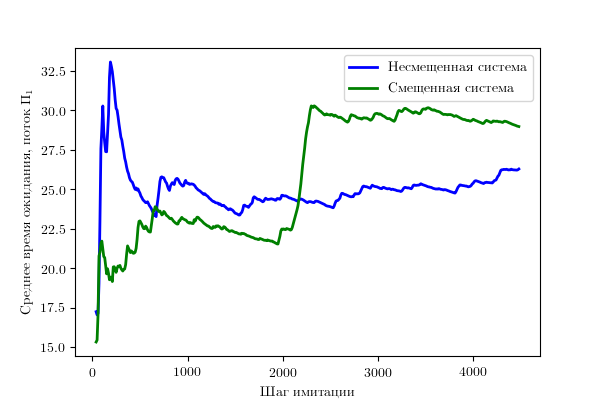
\includegraphics[scale=1]{Pictures/pic_firstTimeUntilServ_stationar.png} 
\caption{Динамика среднего времени ожидания произвольного требования потока $\Pi_1$. Система со стационарным режимом}
\label{Experiment:timeUntilServiceFirst:stationar}
\end{figure}

Основной текст программы написан на языке <<C++>> с использованием многофункционального расширяемого текстового редактора <<GNU Emacs $26.1$>> и компилятора <<GNU C++>> (<<g++>>) версии $7.3$. Для визуализации результатов имитационного моделирования использовался язык <<Python>> версии $3.6$. Подводя итог описанному выше алгоритму, программа включает в себя следующие компоненты.
\begin{itemize}
    \item Функция \textit{оптимизации}: 1) в соответствии с конфигурационным файлом формирует сетку управляющих параметров, с которыми будет запускаться имитационное моделирование; 2) для фиксированного набора параметров инициирует запуск имитации.
    \item Функция \textit{проверки стационарности} системы: 1) производит заданное количество итераций работы алгоритма для смещенной и несмещенной систем; 2) на каждой итерации проверяет близость характеристик смещенной и несмещенной систем и 3) фиксирует факт вступления систем в стационарный режим.
    \item Функция \textit{проведения итерации} системы: 1) осуществляет переключение состояний устройства и подсчет статистики их посещений; 2) осуществляет переключение состояний очередей и сбор статистик, связанных с размерами очередей; 3) с помощью генератора псевдослучайных чисел формирует значения величин, определяющих новые требования потоков $\Pi_1$ и $\Pi_3$, а также принимает решение об уже обслуженных требованиях.
    \item Функция \textit{оценки эффективности работы} системы: 1) аггрегирует характеристики эффективности, подсчитанные для несмещенной системы во время нахождения в стационарном режиме; 2) запись полученных результатов в файл и вывод необходимой информации на экран.
    \item Функция \textit{отрисовки результатов}: при помощи дополнительных модулей <<mpl\_toolkits>>, <<matplotlib>> языка <<Python>> формирует png-изображение, содержащее график результатов работы программы для различных управляющих параметров.
\end{itemize}

\begin{figure}[t]
\centering
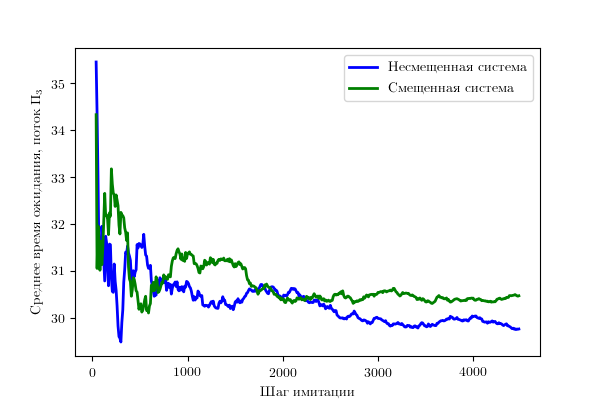
\includegraphics[scale=1]{Pictures/pic_secondTimeUntilServ_stationar.png} 
\caption{Динамика среднего времени ожидания произвольного требования потока $\Pi_3$. Система со стационарным режимом}
\label{Experiment:timeUntilServiceSecond:stationar}
\end{figure}
Опишем используемые в модели величины.
Зафиксируем индекс $j\in \{1, 3\}$, соответствующий номеру потока, и индекс $n=1$, $2$, $\ldots$, соответствующий очередному такту работы управляющей системы.

\begin{figure}[t]
\centering
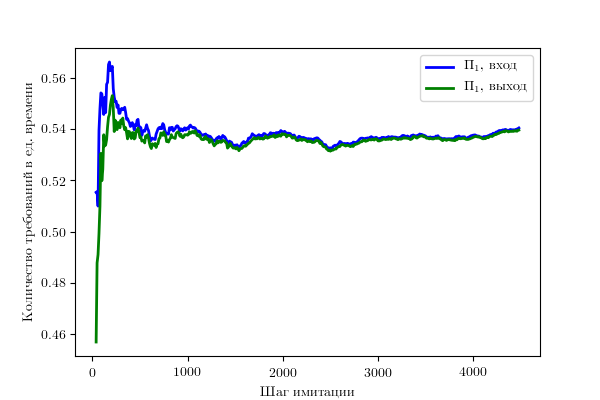
\includegraphics[scale=1]{Dissertation/Work_structured/Pictures/pic_inputOutputFirstFlow_stationar.png}
\caption{Динамика среднего числа поступивших и ушедших требований потока $\Pi_1$  за единицу времени. Система со стационарным режимом}
\label{Experiment:inputOutputFirstFlow:stationar}
\end{figure}
 При моделировании наблюдаются значения следующих статистик: $t_n$~--- продолжительность такта с номером $n$; $\gamma_{j,\nu}^+$ и $\gamma_{j,\nu}^0$~--- для смещенной и несмещенной систем соответственно время ожидания  автомобиля $\nu$ потока $\Pi_j$, $\nu=0$, $1$, $\ldots$;
 $\alpha^{+}_{\text{in},j,n}$ и $\alpha^{0}_{\text{in}, j,n}$~--- количество автомобилей потока $\Pi_j$, которые поступили за такт с номером $n$, в смещенной и несмещенной системах соответственно; 
 $\alpha^{+}_{\text{out},j,n}$ и $\alpha^{0}_{\text{out},j,n}$~--- количество автомобилей потока $\Pi_j$, которые закончили обслуживание на такте $n$ для смещенной и несмещенной систем соответственно;  $\zeta_{j,\nu}$~--- время, которое автомобиль с номером $\nu$ потока $\Pi_j$ провело с момента его прихода в систему и до момента его выхода; $\beta_{j,n}$~--- количество автомобилей, которые находятся в очереди $O_j$ при условии, что  очередь $O_j$ только что начала обслуживаться ($\beta_{j,n}=0$ в остальных случаях). Отметим, что время $\zeta_{1,\nu}$ нахождения в системе автомобиля потока $\Pi_1$ в том числе включает в себя время нахождения в системе его в качестве автомобиля потока $\Pi_2$ и потока $\Pi_4$. При совершении очередного события в системе происходит его обработка и изменение соответствующих отслеживаемых величин. В случае, если в течение определенного количества тактов (авторами экспериментально подобрано значение $100000$) стационарный режим в системе не обнаружен, то процесс имитации заканчивается. Однако, если система входит в стационарный режим, то в течение фиксированного количества тактов (авторами также экспериментально подобрано значение $100000$) происходит подсчет характеристик эффективности функционирования системы.




\begin{figure}[t]
\centering
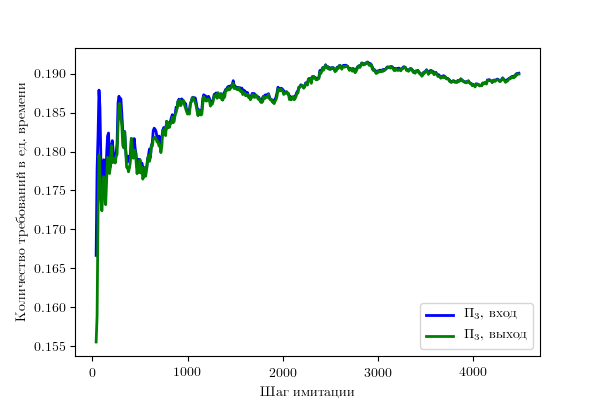
\includegraphics[scale=1]{Dissertation/Work_structured/Pictures/pic_inputOutputSecondFlow_stationar.png}
\caption{Динамика среднего числа поступивших и ушедших требований потока $\Pi_3$ за единицу времени. Система со стационарным режимом}
\label{Experiment:inputOutputSecondFlow:stationar}
\end{figure}

\section{Алгоритм определения момента достижения стационарного режима}
Как правило, под стационарным режимом на содержательном уровне понимают такой режим функционирования системы, устанавливающийся с течением времени, при котором выделенные ее характеристики в среднем остаются неизменными. Идея алгоритма определения момента достижения  такого режима в данной работе заключается в следующем. Наблюдаем одновременно за динамикой смещенной и несмещенной систем и считаем для каждой из них некоторые усредненные величины. Момент, когда эти величины станут достаточно близки, считаем моментом окончания переходных процессов. 

Детали алгоритма будем сопровождать результатами экспериментов, проведенных со следующими наборами параметров:
\begin{itemize}
    \item $\boldsymbol{\lambda_1\in \{0.3, 0.4\}}$, $p_{1}^{(1)}=0.4$, $p_{2}^{(1)}=0.4$, $p_{3}^{(1)}=0.2$, $p_{\nu}^{(1)}=0$, $\nu > 3$;
    \item $(\widetilde{T}^{(1,1)}, \widetilde{T}^{(1,2)})=(30,30)$, $\mu_1 = 1.2$, $\mu_2 = 1.3$;
    \item $\lambda_3=0.1$, $p_{1}^{(3)}=0.4$, $p_{2}^{(3)}=0.3$, $p_{3}^{(1)}=0.3$, $p_{\nu}^{(3)}=0$, $\nu > 3$;
        \item $\mu_4= 0.08$.
\end{itemize}
Здесь представлены два набора параметров, которые отличаются лишь значением параметра $\lambda_1$, выделенным жирным шрифтом. Причем случай $\lambda_1=0.3$ соответствует системе, для которой программно был зафиксирован стационарный режим, а случай $\lambda_1=0.4$~--- системе, для которой стационарный режим обнаружен не был.

\begin{figure}[t]
\centering
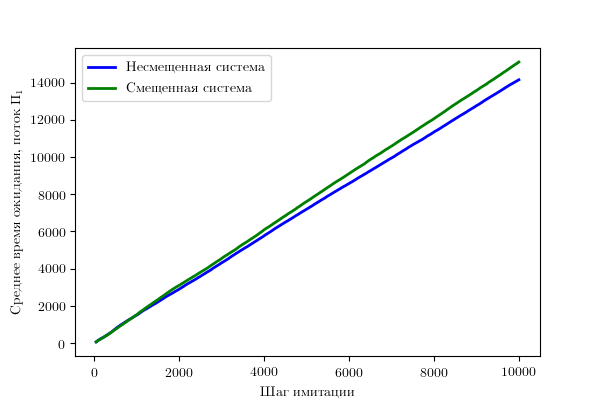
\includegraphics[scale=1]{Dissertation/Work_structured/Pictures/pic_firstTimeUntilServ.png}
\caption{Динамика среднего времени ожидания произвольного требования потока $\Pi_1$. Система без стационарного режима}
\label{Experiment:timeUntilServiceSecond:nonstationar}
\end{figure}

Перейдем к формализации алгоритма. Зафиксируем параметры метода:  $1 > \delta_1$, $1 < \delta_2$ и $1 < \delta_3$. В конце каждого такта будем считать значения 
\begin{equation}
   \gamma_{j,\cdot}^0 = \frac{1}{\tilde{\mathcal{V}}_j^0}\sum_{\nu} \gamma_{j,\nu}^0, \quad \gamma_{j,\cdot}^+ = \frac{1}{\tilde{\mathcal{V}}_j^+}\sum_{\nu} \gamma_{j,\nu}^+,
\end{equation}
среднего времени ожидания обслуживания требований потока $\Pi_j$, $j=1,3$, в несмещенной и смещенной системах соответственно. Динамика времен ожидания для конкретной системы со стационарным режимом при $\lambda_1=0.3$ приведена на рисунках \ref{Experiment:timeUntilServiceFirst:stationar} (для требований потока $\Pi_1$) и \ref{Experiment:timeUntilServiceSecond:stationar} (для требований потока $\Pi_3$).



Для большей устойчивости алгоритма принятия решения о наступлении стационарного режима в несмещенной системе будем следить за количеством требований во входящем и выходящем потоков:
\begin{equation}
    F^{0}_{\text{in},1} = \sum_n \alpha^{0}_{\text{in},1,n}, \quad 
    F^{0}_{\text{out},4} = \sum_n \alpha^{0}_{\text{out},4,n},
\end{equation}
\begin{equation}
    F^{0}_{\text{in},3} = \sum_n \alpha^{0}_{\text{in},3,n}, \quad 
    F^{0}_{\text{out},3} = \sum_n \alpha^{0}_{\text{out},3,n}.
\end{equation}
Для системы со стационарным режимом ожидается, что среднее число требований, пришедших в систему в единицу времени, $F^{0}_{\text{in},1}$ и $F^{0}_{\text{in},3}$, не будет существенно превышать среднее число требований, $ F^{0}_{\text{out},4}$ и $F^{0}_{\text{out},3}$ соответственно, покинувших систему за единицу времени. Поскольку при поступлении в систему требования потока $\Pi_1$ проходят дополнительные этапы обслуживания~--- в качестве требований потока $\Pi_2$ и $\Pi_4$,~--- то количество требований потока $\Pi_1$, покинувших систему, целесообразно считать по выходному потоку $\Pi_4^{\text{out}}$. Динамика соответствующих величин представлена на рисунках \ref{Experiment:inputOutputFirstFlow:stationar} и \ref{Experiment:inputOutputSecondFlow:stationar}.

\begin{figure}[t]
\centering
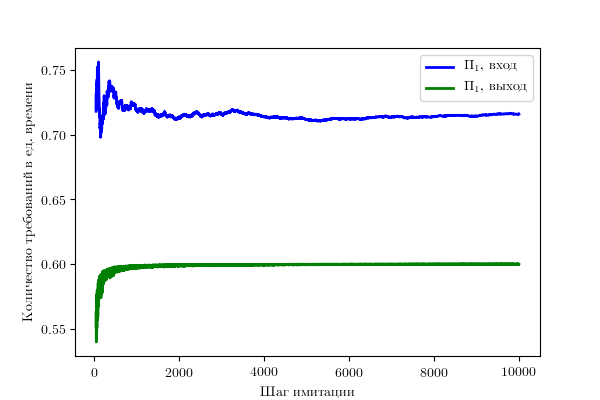
\includegraphics[scale=1]{Dissertation/Work_structured/Pictures/pic_inputOutputFirstFlow.png}
\caption{Динамика среднего числа поступивших и ушедших требований потока $\Pi_3$ за единицу времени. Система со стационарным режимом}
\label{Experiment:inputOutputFirstFlow}
\end{figure}




Окончательное решение о достижении системой стационарного режима будет приниматься в случае, если выполнены следующие неравенства:
\begin{equation}
    \frac{|\gamma_{j,\cdot}^0 - \gamma_{j,\cdot}^+|}{\gamma_{j,\cdot}^0} < \delta_1, \quad
    \frac{F^{0}_{\text{in},1}}{F^{0}_{\text{out},4}} < \delta_2, \quad 
    \frac{F^{0}_{\text{in},3}}{F^{0}_{\text{out},3}} < \delta_3.
\end{equation}

Рассмотрим систему, в которой некоторые очереди неограниченно возрастают и, следовательно, стационарный режим достигнут быть не может. Проанализируем динамику среднего времени ожидания произвольного требования в смещенной и несмещенной системах (рис.~\ref{Experiment:timeUntilServiceSecond:nonstationar}).  Как видно из рисунка, величины $\gamma_{j,\cdot}^0$ и $ \gamma_{j,\cdot}^+$ неограниченно возрастают, причем с похожей скоростью. Поэтому величина $\frac{|\gamma_{j,\cdot}^0 - \gamma_{j,\cdot}^+|}{\gamma_{j,\cdot}^0} $ будет небольшой за счет большого знаменателя и относительно небольшого числителя. 


\begin{figure}[h]
\centering
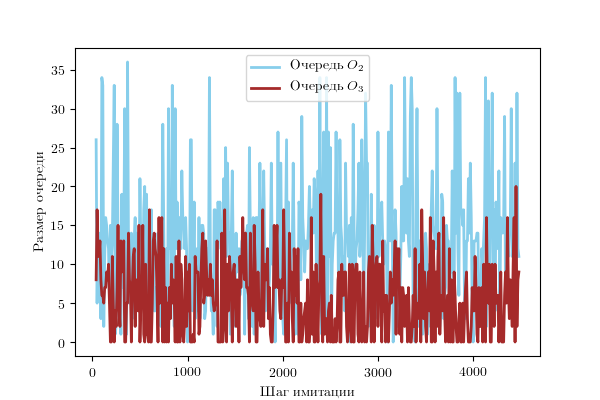
\includegraphics[scale=1]{Dissertation/Work_structured/Pictures/pic_queues_2_stationar.png}
\caption{Динамика длин очередей $O_2$ и $O_3$ второго перекрестка. Система со стационарным режимом}
\label{Experiment:queues:2:stationar}
\end{figure}
Для учета подобных случаев при фиксации факта наличия или отсутствия стационарного режима использовались средние количества входящих и выходящих требований в единицу времени по потокам $\Pi_1$ и $\Pi_3$. Динамика соответствующих величин $F^{0}_{\text{in},1}$ и $F^{0}_{\text{out},4} $ для потока $\Pi_1$ представлена на рисунке~\ref{Experiment:inputOutputFirstFlow}. Из графика видно, что количество $F^{0}_{\text{in},1}$ входящих требований в единицу времени заметно превышает количество $F^{0}_{\text{out},4}$ выходящих требований в единицу времени, поэтому неравенство $\frac{F^{0}_{\text{in},1}}{F^{0}_{\text{out},4}} < \delta_2$ не сможет быть выполнено. 


\section{Показатели качества работы системы}
Как было сказано ранее, важнейшими характеристиками работы системы являются размер очередей и средние времена нахождения требований в системе. Здесь, как и в предыдущем пункте, в качестве примера будем рассматривать запуски программ с теми же двумя наборами параметров, отличающиеся лишь параметром $\Lambda_1$. Для системы со стационарным режимом динамика длин очередей второго перекрестка $O_2$ и $O_3$ представлена на рисунке~\ref{Experiment:queues:2:stationar}. Динамика длины очереди первого перекрестка $O_1$ и длины промежуточной очереди $O_4$ представлены на рисунке~\ref{Experiment:queues:1:stationar}.

\begin{figure}[h]
\centering
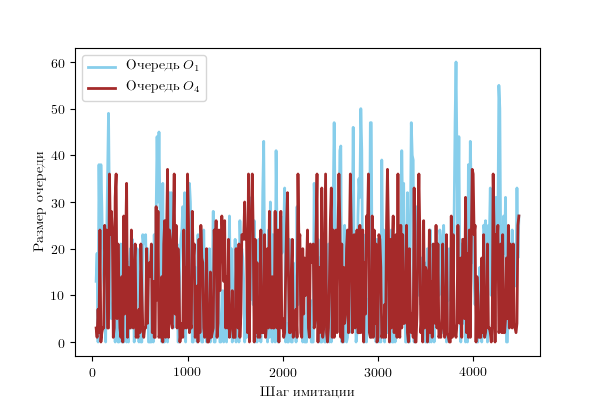
\includegraphics[scale=1]{Dissertation/Work_structured/Pictures/pic_queues_1_stationar.png}
\caption{Динамика длины очереди первого перекрестка $O_1$ и длины промежуточной очереди $O_4$. Система со стационарным режимом}
\label{Experiment:queues:1:stationar}
\end{figure}
Как видно из графиков, длины очередей колеблются между нулем и некоторым конечным числом, что <<подсказывает>> о существовании в такой системе стационарного режима.

%
С другой стороны, при наблюдении за длинами очередей в системе без стационарного режима, величина некоторых очередей может неограниченно возрастать (см. рис.~\ref{Experiment:queues:1:nonstationar}).
\begin{figure}[h]
\centering
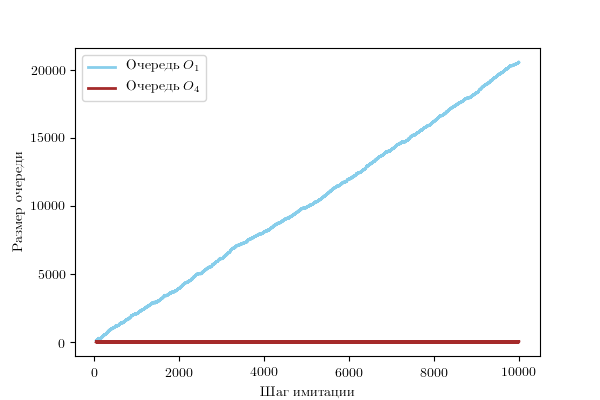
\includegraphics[scale=1]{Dissertation/Work_structured/Pictures/pic_queues_1.png}
\caption{Динамика длины очереди первого перекрестка $O_1$ и длины промежуточной очереди $O_4$. Система без стационарного режима}
\label{Experiment:queues:1:nonstationar}
\end{figure}

После того, как стационарный режим в системе достигнут, можно приступать к оценке основных показателей качества функционирования системы. С этой целью продолжается процесс имитации, но только для несмещенной системы. Необходимо получить оценки для математического ожидания времени пребывания произвольного требования потока $\Pi_j$, $j\in \{1, 3\}$.
%и математического ожидания количества требований в очереди $O_j$ в момент перехода обслуживающего устройства в состояние $^j\Gamma$ на произвольном цикле стационарного режима работы системы. 
За основу можно взять известные в теории вероятностей и математической статистике оценки соответствующих количественных характеристик. Оценки для времени пребывания в системе можно было бы построить по наблюдениям за каждым обслуженным требованием выделенной реализации потока $\Pi_j$.
%, а оценки для количества требований в очереди при переходе к состоянию обслуживания -- по наблюдениям за этой величиной на каждом цикле одной реализации. 
Итак, для каждого $j=1,3$  предлагаются следующие оценки для показателей качества работы системы по потоку $\Pi_j$ :
\begin{itemize}
    \item $\hat{E}\gamma_{j}=\frac{1}{\tilde{\mathcal{V}}_j}\sum_{\nu}\zeta_{j,\nu}$  -- оценка математического ожидания времени пребывания в системе произвольного требования потока $\Pi_j$.
\end{itemize}
Динамика среднего времени пребывания в системе для рассматриваемого примера изображена на рисунке~\ref{Experiment:serv:stationar}.
\begin{figure}[h]
\centering
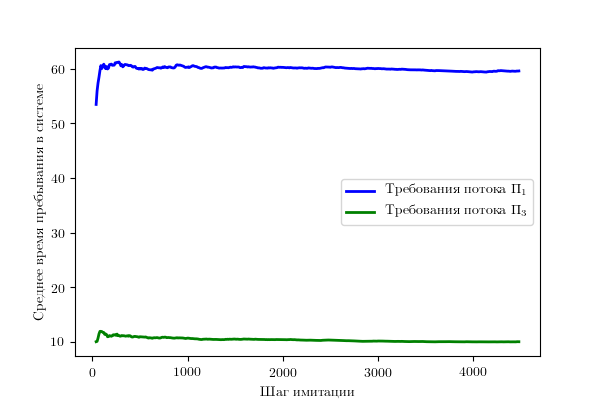
\includegraphics[scale=1]{Dissertation/Work_structured/Pictures/pic_serv_1_stationar.png}
\caption{Динамика среднего времени пребывания требований в системе. Система со стационарным режимом}
\label{Experiment:serv:stationar}
\end{figure}
%
Кроме того, имеет смысл получить оценки, характеризующие работу системы не по отдельному потоку, а для системы в целом. Для этого предлагается строить средние взвешенные оценки, где в качестве веса отдельному потоку приписывается интенсивность поступления его требований, т.е. величина, равная $\lambda_j \sum_{\nu\geqslant1}\nu p_{\nu}^{(j)}$. Итак, имеем результирующую оценку целевой функции
\begin{itemize}
    \item $\hat{E}\gamma=\frac{\sum_{j\in\{1,3\}} (\lambda_j \sum_{\nu\geqslant1}\nu p_{\nu}^{(j)})\hat{E}\gamma_{j} }{\sum_{j\in\{1,3\}} \lambda_j \sum_{\nu\geqslant1}\nu p_{\nu}^{(j)}}$.
\end{itemize}


\section{Анализ области стационарности системы}
Для анализа функционирования тандема перекрестков были зафиксированы следующие параметры:
\begin{itemize}
    \item $\lambda_1=0.35$, $p_{1}^{(1)}=0.4$, $p_{2}^{(1)}=0.4$, $p_{3}^{(1)}=0.2$, $p_{\nu}^{(1)}=0$, $\nu > 3$;
    \item $(\widetilde{T}^{(1,1)}, \widetilde{T}^{(1,2)})=(20,10)$, $\mu_1 = 1.2$;
    \item $\boldsymbol{ \lambda_3=\{0.1, 0.2\}}$, $p_{1}^{(3)}=0.4$, $p_{2}^{(3)}=0.3$, $p_{3}^{(1)}=0.3$, $p_{\nu}^{(3)}=0$, $\nu > 3$;
        \item $\mu_4= 0.001$.
\end{itemize}
Данные наборы параметров уже упоминались выше. Здесь представлены два набора параметров, отличающихся лишь интенсивностью $\boldsymbol{\lambda_3}$ поступления групп требований по потоку $\Pi_3$. Для алгоритма управления перекрестками зафиксируем длительность $\widetilde{T}^{(2,3)}=10$ продления зеленого сигнала светофора для потока $\Pi_2$ и порог $L=10$ продления.

При фиксированном наборе параметров ($\lambda_3 = 0.1$ либо $\lambda_3=0.2$) проводилась серия экспериментов, в которых перебирались значения для длительности обслуживания  $\widetilde{T}^{(2,1)} = \{1, 5, 9, \ldots, 97\}$ требований потока $\Pi_3$ и длительности обслуживания $\widetilde{T}^{(2,2)} = \{1, 5, 9, \ldots, 97\}$ потока $\Pi_2$.

%0_1_thres_10_target
\begin{figure}[h]
\centering
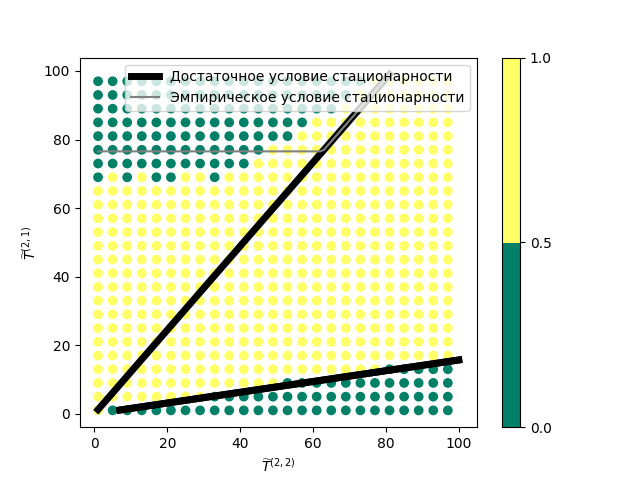
\includegraphics[scale=0.85]{Pictures/0_1_thres_10_target_fact.png} 
\caption{Области стационарности системы. $\lambda_3=0.1$, $L=10$}
\label{Experiment:stationar}
\end{figure}
На рис.~\ref{Experiment:stationar} представлены результаты экспериментов. По осям координат отложены значения $\widetilde T^{(2,1)}$ длительности обслуживания требований потока $\Pi_3$ и значения $\widetilde T^{(2,2)}$ длительности обслуживания требований потока $\Pi_2$. Желтым цветом обозначены точки, в которых было определено достижение системой стационарного режима. Темно-зеленым цветом обозначены случаи отсутствия стационарности. Кроме того на графике черным цветом изображены границы области стационарности, полученная из достаточных условий теоремы~\ref{sufficient:double:theorem}. 

Из графика видно, что желтая область выходит далеко за границы черных линий. Это свидетельствует о том, что достаточное условие, полученное в работе аналитически, не является необходимым. Ввод дополнительного режима продления по высоко приоритетному потоку при отсутвии большого числа требований по низкоприоритетному потоку позволяет существенно расширить область стационарности системы. Интуитивно данный результат ожидаем: при отсутствии требований по одному из потоков, другой поток получает дополнительный временной <<запас>> для обслуживания за счет продления.

Также на графике изображена область, ограниченная серой линией. Эта область получена эмпирическими рассуждениями и дает <<примерную>> оценку области стационарности для системы с продлением. Рассуждения для вывода этой границы основаны на подсчете <<среднего>> количества времени, освобождающегося для обслуживания требований потока $\Pi_2$ за счет продления.

\begin{figure}[h]
\centering
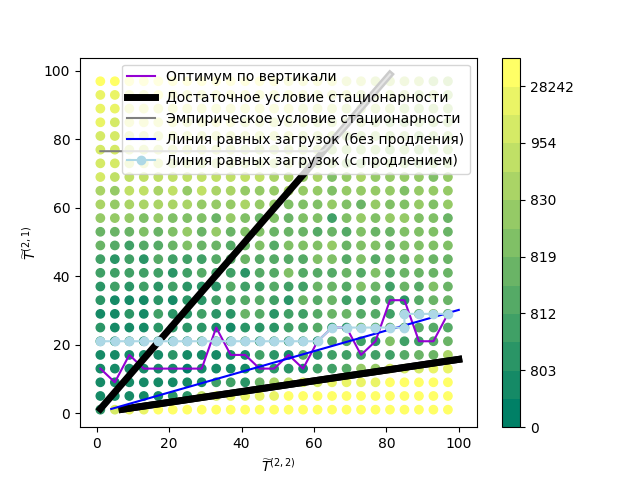
\includegraphics[scale=0.9]{Pictures/0_1_thres_10_target.png} 
\caption{Поиск оптимальных параметров системы}
\label{Experiment:targets}
\end{figure}


Более детально результаты эксперимента представлены на рис.~\ref{Experiment:targets}. На этом рисунке каждому эксперименту соответствует посчитанная оценка средневзвешенной длительности ожидания одного требования. Чем более темным является цвет точки~--- тем лучше. Кроме присутствовавших на предыдущем рисунке границ, здесь присутствуют линии равных загрузок для случая циклического управления (синий цвет) и для случая циклического управления с продлением (голубой цвет). В работах \cite{Fedotkin:2009} и \cite{FedotkinRachinskaya:2016} было отмечено, что оптимальные значение параметров с точки зрения средневзвешенного времени пребывания находится вблизи ломаной равных загрузок. При условии отсутствия продления ($\widetilde T^{(2,3)}=0$),  под загрузкой системы, например, по потоку $\Pi_1$ естественно понимать величину
\begin{equation}
\frac{(\widetilde T^{(2,1)} + \widetilde T^{(2,2)})\lambda_1 \sum_{\nu\geqslant 1}\nu p_{\nu}^{(1)}}{[\mu_2 \widetilde T^{(2,2)}]}.
\end{equation}
Тогда ломаную равных загрузок определим из условия равенства загрузки системы по потокам $\Pi_1$ и $\Pi_3$:
\begin{equation}
\frac{(\widetilde T^{(2,1)} +\widetilde T^{(2,2)})\lambda_1 \sum_{\nu\geqslant 1}\nu p_{\nu}^{(1)}}{[\mu_2 \widetilde T^{(2,2)}]}=
    \frac{(\widetilde T^{(2,1)} + \widetilde T^{(2,2)})\lambda_3 \sum_{\nu\geqslant 1}\nu p_{\nu}^{(3)}}{[\mu_3 \widetilde T^{(2,1)}]}
\end{equation}
График этой кривой изображен на рисунке~\ref{Experiment:targets} синим цветом. 

Далее встает вопрос о том, что считать загрузкой системы в случае присутствия продления по низкоприоритетному потоку $\Pi_3$. В данной работе под загрузкой будем понимать отношение общего числа пришедших требований по потоку ($\Pi_1$ или $\Pi_3$) к общему числу обслуженных требований по этому потоку. Аналитически посчитать эти величины сложно, поэтому на графике представлена кривая равных загрузок, посчитанная на основе экспериментальных данных. Как видно из рисунка, такая кривая лучше <<следует>> за оптимальными значениями параметров, нежели кривая равных загрузок для циклического алгоритма.
\begin{figure*}
\begin{multicols}{2}
    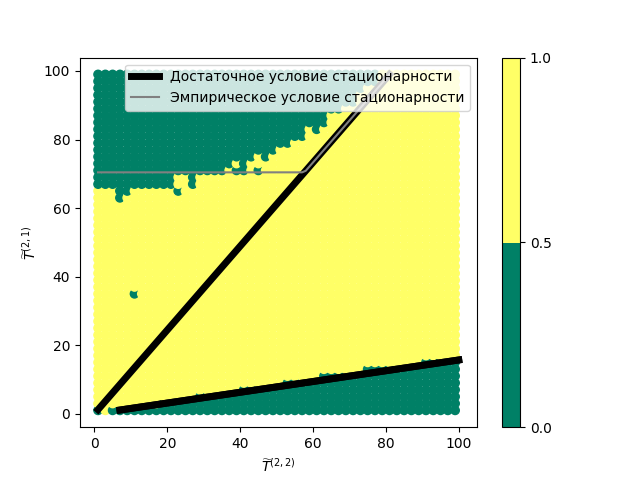
\includegraphics[width=1.2\linewidth]{Pictures/0_1_thres_10_fact.png}\par 
    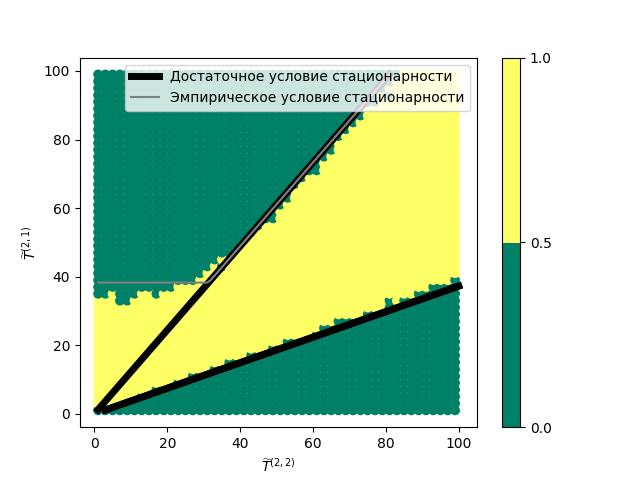
\includegraphics[width=1.2\linewidth]{Pictures/0_2_thres_10_fact.png}\par 
    \end{multicols}
\caption{Области стационарности для разных значений $\lambda_1$. Слева $\lambda_1=0.1$, справа $\lambda_1=0.2$}
\label{Experiment:intensities}
\end{figure*}

Поясним, что значит кривая равных загрузок лучше <<следует>> за оптимальными значениями параметров. Поставим задачу при фикисированном значении времени обслуживания потока $\Pi_2$ (величина $\widetilde T^{(2,2)}$ на рис.~\ref{Experiment:targets}) найти такое значение времени обслуживания потока $\Pi_3$ (величина $\widetilde T^{(2,1)}$ на рис.~\ref{Experiment:targets}), при котором достигается минимум средневзвешенного времени пребывания требования в системе. Фиолетовая линия на рис.~\ref{Experiment:targets} демонстрирует динамику этих значений при изменении времен $\widetilde T^{(2,2)}$. Видно, что <<в среднем>> голубая линия лучше аппроксимирует фиолетовую кривую, чем синяя. Особенно в окрестности прямой $\widetilde T^{(2,2)}=0$. 

\begin{figure*}
\begin{multicols}{2}
    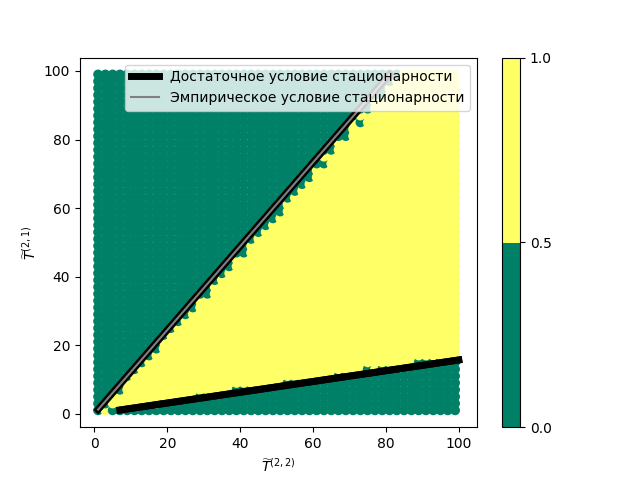
\includegraphics[width=1.15\linewidth]{Pictures/0_1_thres_-1_fact.png}\par 
    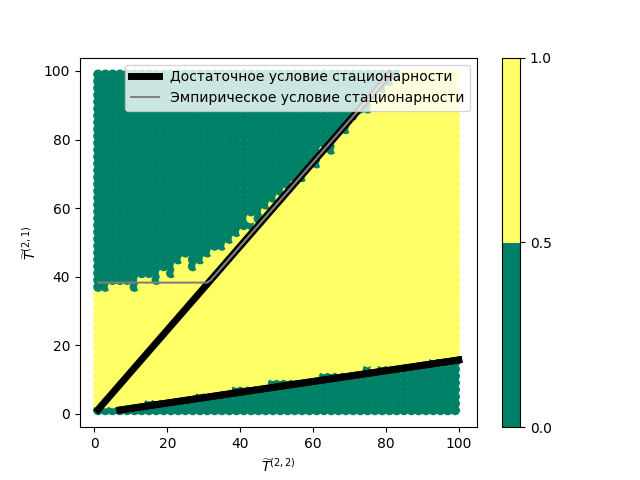
\includegraphics[width=1.15\linewidth]{Pictures/0_1_thres_5_fact.png}\par 
    \end{multicols}
\begin{multicols}{2}
    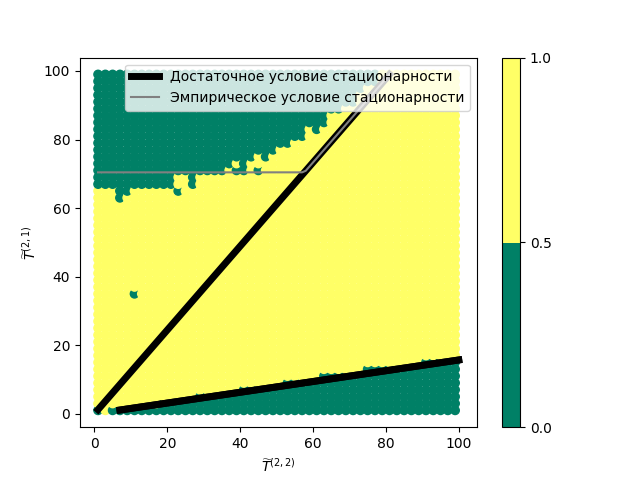
\includegraphics[width=1.15\linewidth]{Pictures/0_1_thres_10_fact.png}\par
    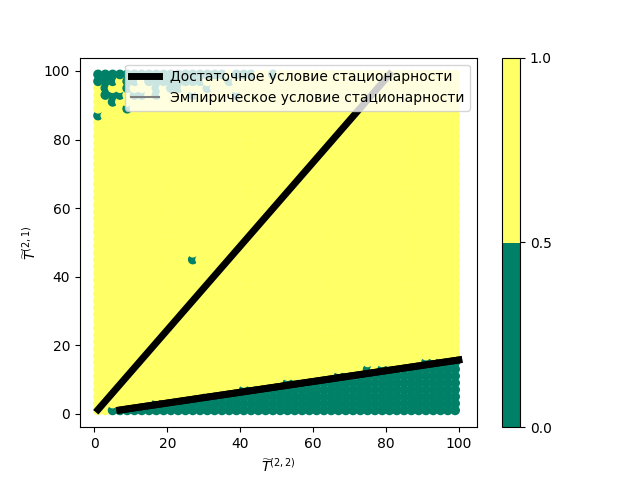
\includegraphics[width=1.15\linewidth]{Pictures/0_1_thres_15_fact.png}\par
\end{multicols}
\caption{Области стационарности для разных значений $L$. Слева-направо, сверху-вниз $L=-1$; $5$; $10$; $15$}
\label{different:thres}
\end{figure*}
Завершая анализ экспериментальных данных, отметим следующее.
\begin{itemize}
    \item При увеличении интенсивности потока $\Pi_2$ (или, что то же самое, интенсивности потока $\Pi_1$), область стационарности сужается (см.~рис.~\ref{Experiment:intensities}).
    \item С увеличением порога $L$ продления, область стационарности увеличивается (см.~рис.~\ref{different:thres}).
\end{itemize}

           % Глава 4
\chapter*{Заключение}						% Заголовок
\addcontentsline{toc}{chapter}{Заключение}	% Добавляем его в оглавление

%% Согласно ГОСТ Р 7.0.11-2011:
%% 5.3.3 В заключении диссертации излагают итоги выполненного исследования, рекомендации, перспективы дальнейшей разработки темы.
%% 9.2.3 В заключении автореферата диссертации излагают итоги данного исследования, рекомендации и перспективы дальнейшей разработки темы.
%% Поэтому имеет смысл сделать эту часть общей и загрузить из одного файла в автореферат и в диссертацию:

В приведенной работе был рассмотрен тандем управляющих систем, управление в которых осуществляется по циклическому алгоритму и алгоритму с продлением. Основные результаты работы заключаются в следующем.

    \begin{enumerate}
        \item Построена строгая математическая модель тандема с циклическим алгоритмом управления и алгоритмом с продлением. Отличительной особенностью системы также является немгновенность перемещения требований между системами. 
        \item Доказана марковость случайной последовательности, включающей длину низкоприоритетной очереди. Проведена классификация состояний цепи по арифметическим свойствам переходных вероятностей этой последовательности. А также найдены достаточное и необходимое условия существования стационарного распределения.
        \item Проведен аналогичный анализ для случайной последовательности, включающей очереди первичных требований: доказана ее марковость, проведена классификация состояний и найдено достаточное условие существования стационарного распределения.
        \item Найдено условие ограниченности для последовательности математических ожиданий $    \{( E\varkappa_{4,i}); i \geqslant 0\}$.
        \item Разработана имитационная модель для изучения исходной системы и написана программа ее реализующая.
        \item На основе имитационной модели были подтверждены и расширены результаты, полученные теоретически.
    \end{enumerate}


      % Заключение
%\include{Dissertation/acronyms}        % Список сокращений и условных обозначений
%\chapter*{Словарь терминов}             % Заголовок
\addcontentsline{toc}{chapter}{Словарь терминов}  % Добавляем его в оглавление

\textbf{TeX} - Cистема компьютерной вёрстки, разработанная американским профессором информатики Дональдом Кнутом

\textbf{Панграмма} - Короткий текст, использующий все или почти все буквы алфавита
      % Словарь терминов
\clearpage                                  % В том числе гарантирует, что список литературы в оглавлении будет с правильным номером страницы
%\hypersetup{ urlcolor=black }               % Ссылки делаем чёрными
%\providecommand*{\BibDash}{}                % В стилях ugost2008 отключаем использование тире как разделителя 
\urlstyle{rm}                               % ссылки URL обычным шрифтом
\ifdefmacro{\microtypesetup}{\microtypesetup{protrusion=false}}{} % не рекомендуется применять пакет микротипографики к автоматически генерируемому списку литературы
\insertbibliofull                           % Подключаем Bib-базы
\ifdefmacro{\microtypesetup}{\microtypesetup{protrusion=true}}{}
\urlstyle{tt}                               % возвращаем установки шрифта ссылок URL
%\hypersetup{ urlcolor={urlcolor} }          % Восстанавливаем цвет ссылок      % Список литературы
%\clearpage
\ifdefmacro{\microtypesetup}{\microtypesetup{protrusion=false}}{} % не рекомендуется применять пакет микротипографики к автоматически генерируемым спискам
\listoffigures  % Список изображений

%%% Список таблиц %%%
% (ГОСТ Р 7.0.11-2011, 5.3.10)
\clearpage
\listoftables   % Список таблиц
\ifdefmacro{\microtypesetup}{\microtypesetup{protrusion=true}}{}
\newpage           % Списки таблиц и изображений (иллюстративный материал)
%\include{Dissertation/appendix}        % Приложения

\end{document}
